%!TEX TS-program = pdflatex
% main.tex -- main dissertation file
%
% Wisconsin dissertation template
% Copyright (c) 2008-2009 William C. Benton.  All rights reserved.
%
% This program can redistributed and/or modified under the terms
% of the LaTeX Project Public License Distributed from CTAN
% archives in directory macros/latex/base/lppl.txt; either
% version 1 of the License, or (at your option) any later version.
%
% This program includes other software that is licensed under the
% terms of the LPPL and the Perl Artistic License; see README for details.
%
% You, the user, still hold the copyright to any document you produce
% with this software (like your dissertation).
%

%%% You'll want ``oneside'' for the deposit version, but probably not for any versions that don't need to meet the UW requirements
\documentclass[12pt,oneside,letterpaper,oldfontcommands]{memoir}
\usepackage[margin=1.2in]{geometry}

\newcommand{\omitme}[1]{}

% preamble.tex -- packages to include
%
% Wisconsin dissertation template
% Copyright (c) 2008 William C. Benton.  All rights reserved.
%
% This program can redistributed and/or modified under the terms
% of the LaTeX Project Public License Distributed from CTAN
% archives in directory macros/latex/base/lppl.txt; either
% version 1 of the License, or (at your option) any later version.
%
% This program includes other software that is licensed under the
% terms of the LPPL and the Perl Artistic License; see README for details.
%
% You, the user, still hold the copyright to any document you produce
% with this software (like your dissertation).

%% You should use natbib
\IfFileExists{natbib.sty}{%
\usepackage{natbib}%
}{}

%% You probably need appendix, if you want appendices
\IfFileExists{appendix.sty}{%
\usepackage{appendix}%
}{}

%% the spacing in memoir is weird, you'll need to use this
\DisemulatePackage{setspace}
\usepackage[onehalfspacing]{setspace}

%% List setup; the ``hanglist`` environment will allow you to have
%% nicely-typeset enumerated lists (i.e. with the numbers hanging in
%% the margins).  You need at least version 2.1 of enumitem.sty.  If
%% you don't have enumitem installed at all, hanglist will just be an
%% alias for enumerate.

%%%%% commented by zihang
\IfFileExists{enumitem.sty}{%
\usepackage[inline]{enumitem}%
}
%\IfFileExists{enumitem.sty}{%
%\usepackage[loadonly]{enumitem}[2007/06/30]%
%\newlist{hanglist}{enumerate}{1}% 
%\setlist[hanglist]{label=\arabic*.}%
%\setlist[hanglist,1]{leftmargin=0pt}%
%}{%
%\newenvironment{hanglist}{\begin{enumerate}}{\end{enumerate}}%
%}
%%%%%%%%%%%%%%%%%%%%%%%%%%%%%%%%

%% Comment out any of these that you don't want
\usepackage{amssymb}
\usepackage{amsmath}
\usepackage{amsthm}
%\usepackage{theorem}
\usepackage{hyperref}

\IfFileExists{mathpartir.sty}{%
\usepackage{mathpartir}%
}{}

%%%%% LISTINGS package and setup
\IfFileExists{listings.sty}{%
\usepackage{listings}%
}{}



%% Get rid of ugly borders around PDF hyperlinks (e.g. for cross-references, bib entries, or URLs)
\hypersetup{pdfborder = 0 0 0}

%% You want microtype.
\IfFileExists{microtype.sty}{%
\usepackage[protrusion=true,expansion=true]{microtype}%
}{}

%\pagestyle{thesisdraft}

% Surround parts of graphics with box
\usepackage{boxedminipage}

%% booktabs (thx to Nate Rosenblum for bringing this beautiful package
%% to my attention)
\IfFileExists{booktabs.sty}{%
\usepackage{booktabs}%
}{}

% This is now the recommended way for checking for PDFLaTeX:
\usepackage{ifpdf}

%% Avoid ugly "Type 3" fonts
\usepackage{lmodern}
\usepackage[LY1]{fontenc}

%% Substitute your favorite serif and sans fonts here....
\IfFileExists{tgpagella.sty}{%
% TeX Gyre pagella, like Palatino
\usepackage{tgpagella}%
}{}

\usepackage[LY1]{eulervm}

\ifpdf
\usepackage[pdftex]{graphicx}
\else
\usepackage{graphicx}
\fi

\usepackage{makeidx}
\makeindex

{\theoremstyle{plain}
\newtheorem{thm}{Theorem}[chapter]
\newtheorem{cor}[thm]{Corollary}
\newtheorem{define}[thm]{Definition}
\newtheorem{exmpl}[thm]{Example}
}
{\theoremstyle{remark}
\newtheorem{rmk}[thm]{Remark}
}

\newtheoremstyle{customsty1}
{3pt}%
{3pt}%
{}% --- body font
{}% --- indent amount
{\bfseries}% --- Theorem head font
{:}% --- Punctuation after head
{.5em}% --- space after head
{}% --- theorem head spec (can be left empty, meaning 'normal')

% Define 'newtheorems' that use ``customsty1''
{\theoremstyle{customsty1} 
}


%%% NB: the ``deposit'' chapter- and page- styles should conform to UW
%%% requirements.  If you are producing a pretty version of your
%%% dissertation for web use later, you will certainly want to make
%%% your own chapter and page styles.

\makechapterstyle{deposit}{%
  \renewcommand{\chapterheadstart}{}
  \renewcommand{\printchaptername}{}
  \renewcommand{\chapternamenum}{}
  \renewcommand{\printchapternum}{\parbox{2em}{\MakeLowercase{\Large\scshape\thechapter{}}} }
  \renewcommand{\afterchapternum}{}
  \renewcommand{\printchaptertitle}[1]{%
  \raggedright\Large\scshape\MakeLowercase{##1}}
  \renewcommand{\afterchaptertitle}{%
  \vskip\onelineskip \hrule\vskip\onelineskip}
}

\makepagestyle{deposit}
 
\makeatletter
 
\renewcommand{\chaptermark}[1]{\markboth{#1}{}}
\renewcommand{\sectionmark}[1]{\markboth{#1}{}}
 
\makeevenfoot{deposit}{}{}{}
\makeoddfoot{deposit}{}{}{}
\makeevenhead{deposit}{\thepage}{}{}
\makeoddhead{deposit}{}{}{\thepage}
\makeatother

%%% set up page numbering for chapter pages to satisfy UW requirements
%%% NB: You will want to delete until the ``SNIP'' mark if you are
%%% making a ``nice'' copy
\copypagestyle{chapter}{plain}
\makeoddfoot{chapter}{}{}{}
\makeevenhead{chapter}{\thepage}{}{}
\makeoddhead{chapter}{}{}{\thepage}
%%% SNIP

%%% bib nonsense
\makeatletter
\newenvironment{wb-bib}[1]{%
  \chapter*{references}
\ifnobibintoc\else 
\phantomsection 
\addcontentsline{toc}{chapter}{References} 
\fi 
\prebibhook
  \begin{bibitemlist}{#1}}{\end{bibitemlist}\postbibhook}

\AtBeginDocument{%
  \@ifpackageloaded{natbib}{% natbib is loaded
    \addtodef{\endthebibliography}{}{\vskip-\lastskip\postbibhook}
    \@ifpackagewith{natbib}{sectionbib}{% with sectionbib option
      \renewcommand{\bibsection}{\@memb@bsec}}%
      {\renewcommand{\bibsection}{\@memb@bchap}}}%
  {}
  \@ifpackagewith{chapterbib}{sectionbib}{%
    \renewcommand{\sectionbib}[2]{}
    \renewcommand{\bibsection}{\@memb@bsec}}{}
}
\makeatother

% defs.tex -- wbepi environment for chapter epigraphs and other useful defs.
%
% Wisconsin dissertation template
% Copyright (c) 2008 William C. Benton.  All rights reserved.
%
% This program can redistributed and/or modified under the terms
% of the LaTeX Project Public License Distributed from CTAN
% archives in directory macros/latex/base/lppl.txt; either
% version 1 of the License, or (at your option) any later version.
%
% This program includes other software that is licensed under the
% terms of the LPPL and the Perl Artistic License; see README for details.
%
% You, the user, still hold the copyright to any document you produce
% with this software (like your dissertation).


%% put lstnewenvironment declarations here, if you're using listings

%% end lstnewenvironment declarations

%% I put convenience definitions that will go in several chapters here

%%%%% begin convenience definitions
\makeatletter
\newcommand{\wb@episource}{}
\newenvironment{wbepi}[1]{\begin{quote}\renewcommand{\wb@episource}{#1}\itshape}{\par\upshape \raggedleft --- \textsc{\wb@episource}\\ \end{quote}}
\makeatother

%%%%% SVN
\IfFileExists{svn-multi.sty}{%
\usepackage{svn-multi}%
%%% Uncomment the second one and comment out the first one if you want
%%% to include subversion revision information in each file.
\newcommand{\vcinfo}{}%
%\newcommand{\vcinfo}{\begin{centering}\fbox{\fbox{\parbox{5in}{Author: \svnauthor\\Revision: \svnfilerev\\Last changed on: \svnfiledate\\URL: \svnkw{HeadURL}}}}\\[1em]\end{centering}}%
}{%
\newcommand{\svnidlong}[4]{}%
\newcommand{\svnfilerev}{}%
\newcommand{\svnauthor}{}%
\newcommand{\svnfiledate}{}%
\newcommand{\svnkw}{}%
\newcommand{\vcinfo}{}%
}
\usepackage{hyperref}

% put bunch of \newcommand below

%%%%% end convenience definitions
 %all packages and definitions can go here
\usepackage[framemethod=TikZ]{mdframed}

% \newtheorem{theorem}{Theorem}
% \newtheorem{lemma}{Lemma}
% \newtheorem{proposition}{Proposition}
% \newtheorem{definition}{Definition}
% \newtheorem{corollary}{Corollary}
% \newtheorem{remark}{Remark}
% \newtheorem{assumption}{Assumption}

\def\EE{\mathbb{E}}
\def\II{\mathbb{I}}
\def\PP{\mathbb{P}}
\def\RR{\mathbb{R}}


\def\cA{\mathcal{A}}
\def\cC{\mathcal{C}}
\def\cD{\mathcal{D}}
\def\cH{\mathcal{H}}
\def\cI{\mathcal{I}}
\def\cL{\mathcal{L}}
\def\cM{\mathcal{M}}
\def\cP{\mathcal{P}}
\def\cS{\mathcal{S}}
\def\cT{\mathcal{T}}
\def\cU{\mathcal{U}}
\def\cW{\mathcal{W}}
\def\cX{\mathcal{X}}
\def\cY{\mathcal{Y}}
\def\cZ{\mathcal{Z}}

\newcommand{\SPD}{\text{SPD}}
\newcommand{\VAR}{\text{VAR}}
\newcommand{\EXP}{\text{Exp}}
\newcommand{\LOG}{\text{Log}}

\mdfdefinestyle{MyFrame}{%
    linecolor=blue!50!white,
    outerlinewidth=1pt,
    roundcorner=5pt,
    innertopmargin=0.5\baselineskip,
    innerbottommargin=0.5\baselineskip,
    innerrightmargin=10pt,
    innerleftmargin=10pt,
    backgroundcolor=blue!10!white}
% thesisdefs.tex

% This is mostly adapted from withesis.cls.  The original copyright
% notice for withesis.cls follows, preceded by two percent signs (%%):

%% withesis.cls
%% LaTeX Style file for the University of Wisconsin-Madison Thesis Format
%% Adapted from the Purdue University Thesis Format
%% Originally by Dave Kraynie
%% Edits by Darrell McCauley
%% Adapted to UW-Madison format by Eric Benedict  (Noted with <EB>)
%% Updated to LaTeX2e by Eric Benedict 24 July 00
%% 
%%=============================================================================
%% Licensed under the Perl Artistic License.
%% see: http://www.ctan.org/tex-archive/help/Catalogue/licenses.artistic.html
%% for more info...
%%=============================================================================

% withesis.cls is available from CTAN.  The modifications to this file
% are also licensed under the Perl Artistic License.

% --wb, 2008

\makeatletter

\newcounter {tocpage}
\newcounter {lofpage}
\newcounter {lotpage}
\newcounter {listofheading}

\newcommand\@thesistitlemedskip{0.2in}
\newcommand\@thesistitlebigskip{0.6in}
\newcommand{\degree}[1]{\gdef\@degree{#1}}
\newcommand{\project}{\gdef\@doctype{A masters project report}}
\newcommand{\prelim}{\gdef\@doctype{A preliminary report}}
\newcommand{\thesis}{\gdef\@doctype{A thesis}}
\newcommand{\dissertation}{\gdef\@doctype{A dissertation}}
\newcommand{\department}[1]{\gdef\@department{(#1)}}

\newenvironment{titlepage}
 {\@restonecolfalse\if@twocolumn\@restonecoltrue\onecolumn
  \else \newpage \fi \thispagestyle{empty}
% \c@page\z@ -- deleted: count title page in thesis
}{\if@restonecol\twocolumn \else \newpage \fi}

\gdef\@degree{Doctor of Philosophy}    %Default is PhD
%\gdef\@doctype{A dissertation}         %Default is dissertation
\gdef\@doctype{A preliminary report}


\gdef\@department{(Computer Sciences)} % Default is Electical Engineering
\gdef\@defensedate{10/18/2021 {\color{red}-- in includes/thesisdefs.tex}}% Default is a long time from now.
\gdef\@committee{ \color{red}
  Name FamilyName1, Assistant Professor, Department\\ 
  Name FamilyName2, Professor, Department\\  
  Name FamilyName3, Assistant Professor, Department\\
  Vikas Singh (Advisor), Professor, Biostatistics and Medical Informatics
  }

\renewcommand{\maketitle}{%
  \begin{titlepage}
%-----------------------------------------------------------------------------
% -- The thesis office doesn't like thanks on title page.  Put it in
% -- the acknowledgments.  This is here so you don't have to change
% -- your titlepage when converting from report style. -> from Purdue, but I
%        left it here since it seems compatible with UW-Madison, Eric
%-----------------------------------------------------------------------------
    \def\thanks##1{\typeout{Warning: `thanks' deleted from thesis titlepage.}}
    \let\footnotesize\small \let\footnoterule\relax \setcounter{page}{1}
    \begin{center}
      {\textbf{\expandafter\expandafter{\@title}}} \\[\@thesistitlebigskip]
       by \\[\@thesistitlemedskip]
      \@author \\[\@thesistitlebigskip]
      \@doctype\ submitted in partial fulfillment of \\
      the requirements for the degree of\\[\@thesistitlebigskip]
      \@degree \\[\@thesistitlemedskip]
      \@department \\[\@thesistitlebigskip]
      at the \\[\@thesistitlemedskip]
      UNIVERSITY OF WISCONSIN--MADISON\\[\@thesistitlemedskip]
      \@date
    \end{center}
%    \hspace*{-0.7in}Date of final oral examination: \@defensedate \\[\@thesistitlemedskip]
    \hspace*{-0.4in}Date of preliminary examination: \@defensedate \\[\@thesistitlemedskip]
%    \hspace*{-0.7in}The dissertation is approved by the following members of the 
    \hspace*{-0.4in}The examination is approved by the following members of the 
    Oral Committee:\\
    \@committee
  \end{titlepage}
  \setcounter{footnote}{0}
  \setcounter{page}{1} %title page is NOT counted
  \let\thanks\relax
  \let\maketitle\relax \let\degree\relax \let\project\relax \let\prelim\relax
  \let\department\relax
  \gdef\@thanks{}\gdef\@degree{}\gdef\@doctype{}
  \gdef\@department{}
  %\gdef\@author{}\gdef\@title{}
}


%=============================================================================
% ABSTRACT
%=============================================================================
% The abstract should begin with two single-spaced lines describing
% the author and title in a standard format.  After these lines comes
% the standard abstract.
%=============================================================================
\def\abstract{
  \chapter*{Abstract}
  \addcontentsline{toc}{chapter}{Abstract}
  \relax\markboth{Abstract}{Abstract}}
\def\endabstract{\par\newpage}


%=============================================================================
% UMI ABSTRACT
%=============================================================================
% The UMI abstract should begin with the author and title in a standard format.
% After the author comes the advisor and university. After these lines comes
% a bunch of double spaced text to make up the standard abstract.
% After the abstract, the advisor's approval signature follows.
% This page is not numbered and is delivered seperately to the thesis office.
%=============================================================================

\def\advisortitle#1{\gdef\@advisortitle{#1}}
\def\advisorname#1{\gdef\@advisorname{#1}}
\gdef\@advisortitle{Professor}
\gdef\@advisorname{Cheer E.\ Place}

\def\umiabstract{
             \thispagestyle{empty}
                  \addtocounter{page}{-1}
                \begin{center}
                  {\textbf{\expandafter\uppercase\expandafter{\@title}}}\\
                  \vspace{12pt}
                  \@author \\
                  \vspace{12pt}
                  Under the supervision of \@advisortitle\ \@advisorname\\
                  At the University of Wisconsin-Madison
                \end{center}
}

\def\endumiabstract{\vfill \hfill\@advisorname\par\newpage}


%============================================================================
% VERBATIMFILE
%============================================================================
% \verbatimfile{<filename>}    for verbatim inclusion of a file
% - Note that the precise layout of line breaks in this file is important!
% - added the \singlespace - EB
%============================================================================
\def\verbatimfile#1{\begingroup \singlespace
                    \@verbatim \frenchspacing \@vobeyspaces
                    \input#1 \endgroup
}


%=============================================================================
% SEPARATOR Pages
%   Creates a blank page with a text centered horizontally and vertically.
%   The page is neither counted nor numbered.
%   These pages are required in the thesis format before sections such
%   as appendices, vita, bibliography, etc.
%=============================================================================
\def\separatorpage#1{
  \newpage
  \thispagestyle{empty}
  \addtocounter{page}{-1}
  \null
  \vfil\vfil
  \begin{center}
    {\textbf{#1}}
  \end{center}
  \vfil\vfil
  \newpage}


%=============================================================================
% COPYRIGHTPAGE
%=============================================================================
% The copyright must do the following:
% - start a new page with no number
% - place the copyright text centered at the bottom.
%=============================================================================
\def\copyrightpage{
  \newpage
  \thispagestyle{empty}    % No page number
  \addtocounter{page}{-1}
  \chapter*{}            % Required for \vfill to work
  \begin{center}
   \vfill
   \copyright\ Copyright by \@author\ \@date\\
   All Rights Reserved
  \end{center}}


%=============================================================================
% GLOSSARY
%=============================================================================
% The glossary environment must do the following:
% - produce the table of contents entry for the glossary
% - start a new page with GLOSSARY centered two inches from the top
%=============================================================================
\def\glossary{
  \chapter*{GLOSSARY}
  \addcontentsline{toc}{chapter}{Glossary}}
\def\endglossary{\par\newpage}

%=============================================================================
% NOMENCLATURE
%=============================================================================
% The nomenclature environment must do the following:
% - produce the table of contents entry for the nomenclature section
% - start a new page with NOMENCLATURE centered two inches from the top
%=============================================================================
\def\nomenclature{\separatorpage{DISCARD THIS PAGE}
  \chapter*{Nomenclature}
  \addcontentsline{toc}{chapter}{NOMENCLATURE}}
\def\endnomenclature{\par\newpage}

%=============================================================================
% CONVENTIONS
%=============================================================================
% The conventions environment must do the following:
% - produce the table of contents entry for the nomenclature section
% - start a new page with CONVENTIONS centered two inches from the top
%=============================================================================
\def\conventions{\separatorpage{DISCARD THIS PAGE}
  \chapter*{Conventions}
  \addcontentsline{toc}{chapter}{CONVENTIONS}}
\def\endconventions{\par\newpage}


%=============================================================================
% COLOPHON
%=============================================================================
% The colophon environment must do the following:
% - produce the table of contents entry for the nomenclature section
% - start a new page with COLOPHON centered two inches from the top
%=============================================================================
%\def\colophon{\separatorpage{DISCARD THIS PAGE}
%  \chapter*{Colophon}
%  \addcontentsline{toc}{chapter}{Colophon}}
%\def\endcolophon{\par\newpage}

%=============================================================================
% LIST OF SYMBOLS
%=============================================================================
% The list of symbols environment must do the following:
% - produce the table of contents entry for the list of symbols section
% - start a new page with LIST OF SYMBOLS centered two inches from the top
%=============================================================================
\def\listofsymbols{\separatorpage{DISCARD THIS PAGE}
  \eject
  \chapter*{LIST OF SYMBOLS}
  \addcontentsline{toc}{chapter}{LIST OF SYMBOLS}}
\def\endlistofsymbols{\par\newpage}

%=============================================================================
% VITA
%=============================================================================
% The vita environment must do the following:
% - produce a separator page with the word vita centered
% - produce the table of contents entry for the vita
% - start a new page with VITA centered two inches from the top
%=============================================================================
\def\vita{
%  \separatorpage{VITA}         % UW doesn't require this EB
  \chapter*{VITA}
  \addcontentsline{toc}{chapter}{VITA}}
\def\endvita{\par\newpage}

%=============================================================================
% ACKNOWLEDGMENTS
%=============================================================================
% The acknowledgments environment must do the following:
% - start a new page with ACKNOWLEDGMENTS centered two inches from the top
%=============================================================================
\def\acks{
  \chapter*{Acknowledgments}
}
\def\endacks{\par\newpage}

%=============================================================================
% DEDICATION
%=============================================================================
% The dedication environment must do the following:
% - start a new page
% - center the text vertically
% - include the text in a center environment
%=============================================================================
\def\dedication{
  \newpage
  \null\vfil
  \begin{center}}
\def\enddedication{\end{center}\par\vfil\newpage}

%=============================================================================
% DATE
%=============================================================================
%\def\today{\ifcase\month\or
  %January\or February\or March\or April\or May\or June\or
  %July\or August\or September\or October\or November\or December\fi
  %\space\number\day, \number\year}
\newcount\@testday
\def\today{\@testday=\day
  \ifnum\@testday>30 \advance\@testday by -30
  \else\ifnum\@testday>20 \advance\@testday by -20
  \fi\fi
  \number\day\ \
  \ifcase\month\or
    January \or February \or March \or April \or May \or June \or
    July \or August \or September \or October \or November \or December
    \fi\ \number\year
}


%  Single counter for theorems and theorem-like environments:
\newtheorem{theorem}{Theorem}[chapter]
\newtheorem{assertion}[theorem]{Assertion}
\newtheorem{claim}[theorem]{Claim}
\newtheorem{conjecture}[theorem]{Conjecture}
\newtheorem{corollary}[theorem]{Corollary}
\newtheorem{definition}[theorem]{Definition}
\newtheorem{example}[theorem]{Example}
\newtheorem{figger}[theorem]{Figure}
\newtheorem{lemma}[theorem]{Lemma}
\newtheorem{prop}[theorem]{Proposition}
\newtheorem{remark}[theorem]{Remark}

%=============================================================================
% TABLE OF CONTENTS; LIST OF FIGURES; LIST OF TABLES
%=============================================================================
% In report style, \tableofcontents, \listoffigures, etc. are always
% set in single-column style.  @restonecol is used to keep track of
% whether we need to switch back to double column style after the toc.
%
% The only known problem now is that the first page with the new
% layout is too long.  The problem seems to be that the change to
% textheight doesn't take place on the first page.  Even if it's the
% first line in the table of contents macro.  Presumably the same
% problem also occurs in the lof and lot.
%
% I'm taking a shot at fixing the problem by dropping in a throw-away
% page between the change to the height parameters and the start of
% the chapter.  Isn't elegance wonderful?
%
%=============================================================================

% \def\@tableof#1#2#3#4#5{
% { % limit scope of following declarations!!
%   \@restonecolfalse\if@twocolumn\@restonecoltrue\onecolumn\fi
%   \addtolength{\textheight}{-40pt}       % -24-16
%   \addtolength{\majorheadskip}{-40pt}    % -24-16
%   \addtolength{\headheight}{52pt}        %  36+16
%   \addtolength{\headsep}{-12pt}          % -12
%   \separatorpage{DISCARD THIS PAGE}
%   \chapter*{#1}
%   #5
%   \relax\markboth{#1}{#1}
%   \hbox to \hsize{#2 \hfil Page}
%   \singlespace
%   \setcounter{#3}{0}
%   \setcounter{listofheading}{1}  % change from 0 to 1 by mccauley, 14may93
%   \def\@oddhead{\vbox to \headheight{\vspace{4pt}
%     \hbox to \hsize{\hfil\textrm{\thepage}} \vfil
%     \ifnum\value{#3}=1
%       \ifnum\value{listofheading}=2
%         \hbox to \hsize{Appendix\hfil} \vspace{4pt} \fi
%       \ifnum\value{listofheading}=1
%         \stepcounter{listofheading} \fi
%       \hbox to \hsize{#2 \hfil Page}
%     \else
%       \setcounter{#3}{1}
%     \fi}}
%   \def\@evenhead{\vbox to \headheight{\vspace{4pt}
%     \hbox to \hsize{\textrm{\thepage}\hfil} \vfil
%     \ifnum\value{#3}=1
%       \ifnum\value{listofheading}=2
%         \hbox to \hsize{Appendix\hfil} \vspace{4pt} \fi
%       \ifnum\value{listofheading}=1
%         \stepcounter{listofheading} \fi
%       \hbox to \hsize{#2 \hfil Page}
%     \else
%       \setcounter{#3}{1}
%     \fi}}
%   \@starttoc{#4}  \if@restonecol\twocolumn\fi
%   \newpage
% }}
% 
% \def\tableofcontents{\@tableof{TABLE OF CONTENTS}{}{tocpage}{toc}{}}
% 
% \def\listoffigures{
%   \@tableof{LIST OF FIGURES}{Figure}{lofpage}{lof}
%   {\protect\addcontentsline{toc}{chapter}{LIST OF FIGURES}}}
% 
% \def\listoftables{
%   \@tableof{LIST OF TABLES}{Table}{lotpage}{lot}
%   {\protect\addcontentsline{toc}{chapter}{LIST OF TABLES}}}

%=============================================================================
% BIBLIOGRAPHY
%=============================================================================
% The thebibliography environment executes the following commands:
%
%  o start a new 'chapter' with BIBLIOGRAPHY as the heading
%  o produce a separator page for the bibliography
%
%  \def\newblock{\hskip .11em plus .33em minus -.07em} --
%      Defines the `closed' format, where the blocks (major units of
%      information) of an entry run together.
%
%  \sloppy  -- Used because it's rather hard to do line breaks in
%      bibliographies,
%
%  \sfcode`\.=1000\relax --
%      Causes a `.' (period) not to produce an end-of-sentence space.
%=============================================================================
% \altbibtitle
%   The default title for the References chapter is ``LIST OF REFERENCES''
%   Since some people prefer ``BIBLIOGRAPHY'', the command
%   \altbibtitle has been added to change the chapter title.
%   This command does nothing more than change REFERENCES to BIBLIOGRAPHY
%============================================================================
\def\@bibchaptitle{Bibliography}
\def\altbibtitle{\def\@bibchaptitle{Bibliography}}
\def\thebibliography#1{
  %\separatorpage{\@bibchaptitle}
  \global\@bibpresenttrue
  \chapter*{\@bibchaptitle\markboth{\@bibchaptitle}{\@bibchaptitle}}
  \addcontentsline{toc}{chapter}{\@bibchaptitle}
  \vspace{0.375in}    % added to match 4 line requirement
  \interlinepenalty=10000 % added to prevent breaking of bib entries
  \singlespace\list
  {[\arabic{enumi}]}{\settowidth\labelwidth{[#1]}\leftmargin\labelwidth
    \advance\leftmargin\labelsep \usecounter{enumi}}
  \def\newblock{\hskip .11em plus .33em minus -.07em}
  \sloppy
  \sfcode`\.=1000\relax}
\let\endthebibliography=\endlist



\makeatother


\usepackage[textsize=scriptsize,color=red!25]{todonotes}

\hypersetup{
	colorlinks = true,
	urlcolor = {green}, urlbordercolor = {green},
	citecolor = {blue},
	linkbordercolor = {green}
}

\let\ab\allowbreak
%%%%%%%%%%%%%%%%%%%%%%%%%%%%%%%%%%%%%%%%%%%%%%%%%%%%%%

\title{Identifying Feature, Parameter, and Sample Subsets in Machine Learning and Image Analysis}
\author{Ronak Mehta}
\department{Computer Sciences Department}
\date{2023}

\begin{document}

%%% Uncomment the following if your .bib contains references that you will not  explicitly cite, but that should be in the final bibliography:
% \nocite{*}

\maketitle

\copyrightpage

\pagenumbering{roman}
\begin{acks}
Acknowledgements go here 
% meal replacements, madison metro
% drugs/therapy
% family, forgive
% vikas
% beth, angela, desmond, pradeep
% labmates/collabs hyunwoo seongjae wonhwa vamsi sathya haoliang eric tianyi yuri yunyang xingjian zihang sourav vishnu 
% amfam glenn jeff
% michael newton
% sterling
% commitee fred yongjae 
% mike chris ross bryce 

Work in Chapter 3 was supported in part by NIH grants R01 AG040396, AG021155, EB022883 
and NSF grants DMS 1265202 and CAREER award 1252725.
The authors were also supported by the \href{http://cpcp.wisc.edu/}{UW Center for Predictive Computational Phenotyping} (via BD2K award AI117924) and the \href{http://www.adrc.wisc.edu/}{Wisconsin Alzheimer's Disease Research Center} (AG033514). 
I was supported by a fellowship via training grant award T32LM012413. 
\end{acks}

\tableofcontents
\newpage
\listoffigures
\newpage
\listoftables
\newpage

\listoftodos
\newpage
\begin{abstract}
    Modern machine learning has proven to be extremely effective in aiding and automating a large number of tasks, beginning with simple image recognition, 
    now ranging widely from full language translation and understanding to computer-aided medical diagnosis and drug discovery.
    These advances have largely been enabled
    by significant development in computation schemes and algorithms, that have come alongside
    exponential increases in the scale of 
    training data available.
    Success in these cases is measured directly by performance,
    evaluating some sort of error or accuracy
    that proves to be competitive with even
    domain-level experts.
    Recent research within the field
    has thus now moved to orthogonal, but equally important questions involving 
    robustness to data distribution shifts,
    model fairness, interpretability of
    model outputs, and explainability of 
    model predictions.
    The analysis of these varied questions
    typically look at the learning formulation
    with a finer toothed comb,
    identifying individual elements or groups of elements of interest.
    These ideas all fall under a similar fundamental problem of \textit{finding subsets}, where they be of groups within the population, features of the input, or sections of the model.
    Uniquely shaped by their particular machine learning instantiations, we need methods for identifying \textbf{(1)}  subsets of training samples or subpopulations which have disparate outcomes for a given model, \textbf{(2)} feature subsets that are sufficient or uniquely explain a particular model prediction, and \textbf{(3)} important parameter subsets or paths through neural network models that explicitly describe how a model output was generated.
    In this dissertation,
    we will describe a number of methods for addressing these subset selection problems.
    Developing mathematical tools based primarily on 
    aspects of differential geometry and conditional independence,
    we will demonstrate theoretical and empirical effectiveness of these methods on a wide breadth
    of problems that can be distilled in the manner above, including hypothesis testing with medical imaging, predicting disease progression, machine unlearning, and increasing model fairness.
\end{abstract}

%Modern machine learning has proven to be extremely effective in aiding and automating a large number of tasks, beginning with simple image recognition, now ranging widely from full language translation and understanding to computer-aided medical diagnosis and drug discovery. These advances have largely been enabled by significant development in computation schemes and algorithms, that have come alongsideexponential increases in the scale of training data available. Success in these cases is measured directly by performance,evaluating some sort of error or accuracythat proves to be competitive with evendomain-level experts. Recent research within the fieldhas thus now moved to orthogonal, but equally important questions involving robustness to data distribution shifts, model fairness, interpretability ofmodel outputs, and explainability of model predictions. The analysis of these varied questionstypically look at the learning formulationwith a finer toothed comb,identifying individual elements or groups of elements of interest. These ideas all fall under a similar fundamental problem of finding subsets, where they be of groups within the population, features of the input, or sections of the model. Uniquely shaped by their particular machine learning instantiations, we need methods for identifying (1) subsets of training samples or subpopulations which have disparate outcomes for a given model, (2) feature subsets that are sufficient or uniquely explain a particular model prediction, and (3) important parameter subsets or paths through neural network models that explicitly describe how a model output was generated. In this dissertation, we will describe a number of methods for addressing these subset selection problems. Developing mathematical tools based primarily on aspects of differential geometry and conditional independence, we will demonstrate theoretical and empirical effectiveness of these methods on a wide breadth of problems that can be distilled in the manner above, including hypothesis testing with medical imaging, predicting disease progression, machine unlearning, and increasing model fairness.

\clearpage
\pagenumbering{arabic}
\clearpage
\chapter{Introduction} \label{chap:intro} 

Modern applications of machine learning in a broad range of industrial and consumer-facing systems have become ubiquitous.
Most interactions with daily technologies now intrinsically involve 
a request to some ``smart`` system in the ``cloud'', 
where those interactions range from
a request for map directions 
to simply loading a webpage.
Neural network models, and the recent advances of deep learning,
have enabled these systems that 
make such applications possible.
These models have achieved
human-level performance on learning tasks
including image classification~\citep{resnet,alexnet}, image segmentation~\citep{segmentation}, video analysis~\citep{zhang2016video}, text understanding and generation~\citep{bert,gpt}, and have slowly begun to solve more fundamental scientific problems such as protein folding~\citep{protein} drug discovery~\citep{drugdisc}, and medical diagnosis~\citep{diag}.
While this performance is largely attributed to model size,
the abundance of high quality training data
has equally contributed to real world performance,
enabling model training over millions of real world samples~\citep{imagenet,laion},
and potentially billions of synthetic samples via environment simulation~\citep{mcts}.

While deployment in some domains (recommender systems, object detection) may benefit almost unconditionally from this vastly expanded capability, rightful hesitancy has limited their widespread use in particular applications where impacts on individuals, people, or environments may be at stake.
These ``last mile'' concerns take a few forms.
% Because a completely accurate model is still out of reach, an important question that needs to be answered is: which inputs or individuals are being given incorrect outcomes, and why?
% maybe a sentence suggesting unlearning/removal
In mission critical applications such as medical diagnosis, 
the impact of an error can be extremely large,
even if a misprediction happens extremely infrequently.
Additionally, large scale model training and architecture search
can require exorbitant amounts of energy producing high emissions,
and their scale can limit market participants
to only large actors with vast existing resources.
The accessibility and effectiveness of these models can also vary significantly based on the training data, and disparate outcomes can be exacerbated by existing social inequity.

While existing human or ``natural'' systems that these models aim to assist are not perfect, 
our real world has developed norms and regulations that 
enable them to function.
A medical diagnosis might require a physician to explain what symptoms led them to that particular conclusion.
Energy metering and carbon taxes may be applied to limit
emissions.
Regulatory satisfaction may require 
analysis proving equal opportunity,
or that specific protected classes
are not used in decision making.
% Specifically, these can include ideas as simple as the Hippocratic Oath and medical malpractice insurance, to asking your doctor what symptoms lead them to a particular diagnosis.
These ideas are difficult to directly translate to automated machine learning systems,
but proxies have been identified that we can build upon.

These norms and regulations answer a number of questions we may also try to pose to our machine learning models.
What is the cost to learn this task?
What led to this particular outcome?
Why is this outcome different from another?
% We will explore how these questions can be formulated concretely. 

If the answer to these questions is negative or unknown,  follow-up questions all take an interesting form:
Can we learn a smaller model with similar performance? 
Can we identify the most important features? 
Which individuals or groups are being treated unfairly, and can we change that?
These questions ask us to identify a \textit{subset} of some relevant set, dependent on setting, and this identification is our focus here.

% Moving specifically to machine learning methods,
Taking a step back, let's take a look at a representative system. Figure~\ref{fig:dl} illustrates a typical learning pipeline. 
A dataset is collected and used to train a model, by minimizing the error over
those samples in the dataset (top).
A ``sample'' can be a single measured value, or it can
be a large, highly structured object with many ``features.''
The model is made up of some ``parameters'' that are 
tuned during training to learn a good predictor over the training dataset.
This model is then used to predict, or \textit{infer}, on new
data seen ``in the wild'' (bottom).
Our questions above are formally asking to identify \textit{subsets of these objects}: is a subset of the model parameters sufficient for learning? Which subset of the features are important for a prediction? Which subset of the dataset exhibit a specific attribute?
\begin{figure}
    \centering
    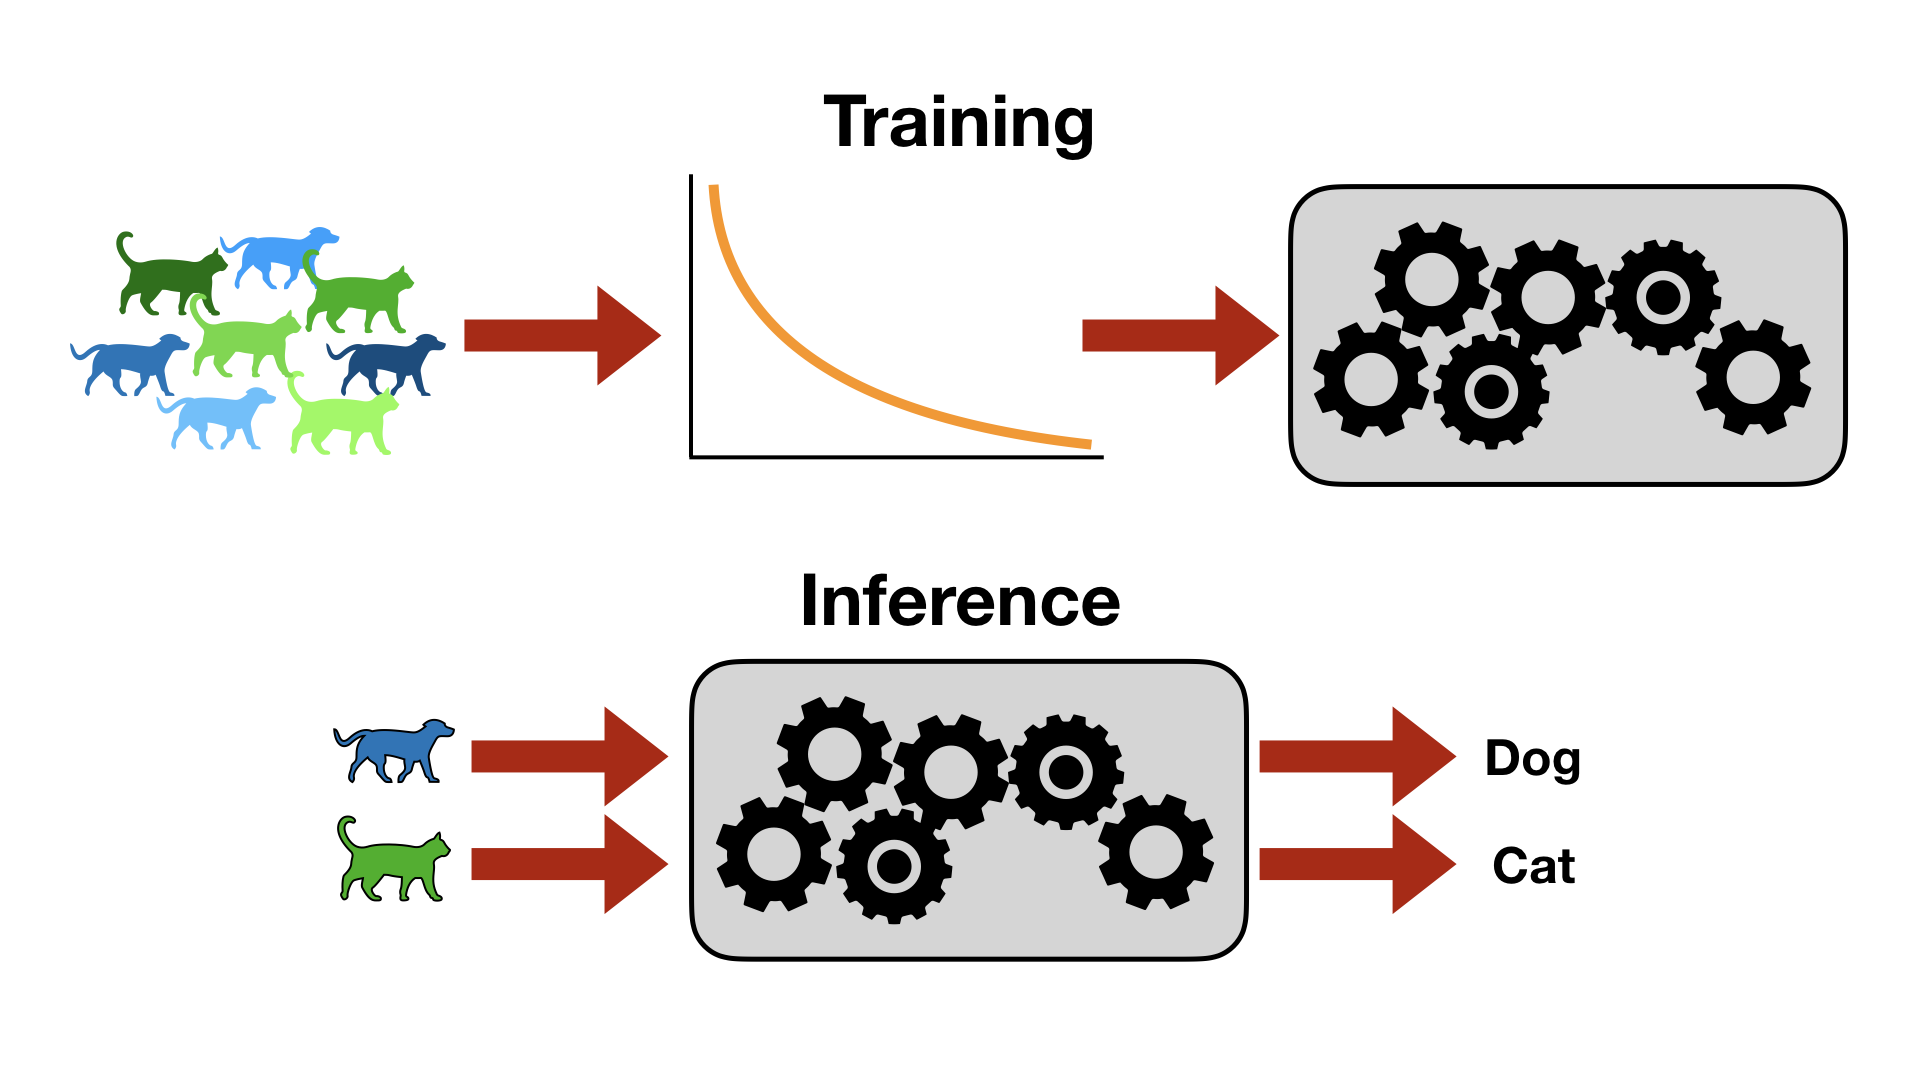
\includegraphics[trim={0 3cm 0 3cm},clip,width=0.95\textwidth]{diss/1_intro/figs/dl.png}
    \caption[Modern machine learning pipelines]{Machine learning training and inference visualization.}
    \label{fig:dl}
\end{figure}

% \textit{Explainability} can be seen as identifying important features of the input, as well as parts of the model (parameters) that ``light up`` for that input. \textit{Fairness} can be evaluated via measures over subsets of the data that correspond to specific groups. 

\begin{mdframed}[style=MyFrame]
\em 
\textbf{This thesis} focuses its main efforts on identifying these important subsets of model, feature, and sample space, to enable answering questions necessary for mainstream adoption of machine learning methods.
\end{mdframed}

% In this dissertation, we explore the sizes of these models, samples, and datasets, and 
% analyze under what situations 
% a smaller \textit{subset} of them may be sufficient or important
% for questions that run parallel to standard performance and accuracy measures.

Let us step a bit deeper into a basic illustrative example. In order to ease understanding, we can first begin with a basic formulation of learning methods, from which the questions above can take specific forms. 
Learning methods typically  try to identify a function mapping (model) that is able to complete a specific task at some high level of profficiency.
% In Figure~\ref{fig:dl}, a model is trained using examples of classification task (top), in order to accurately predict the class of a newly provided input (bottom).
% \begin{figure}
%     \centering
%     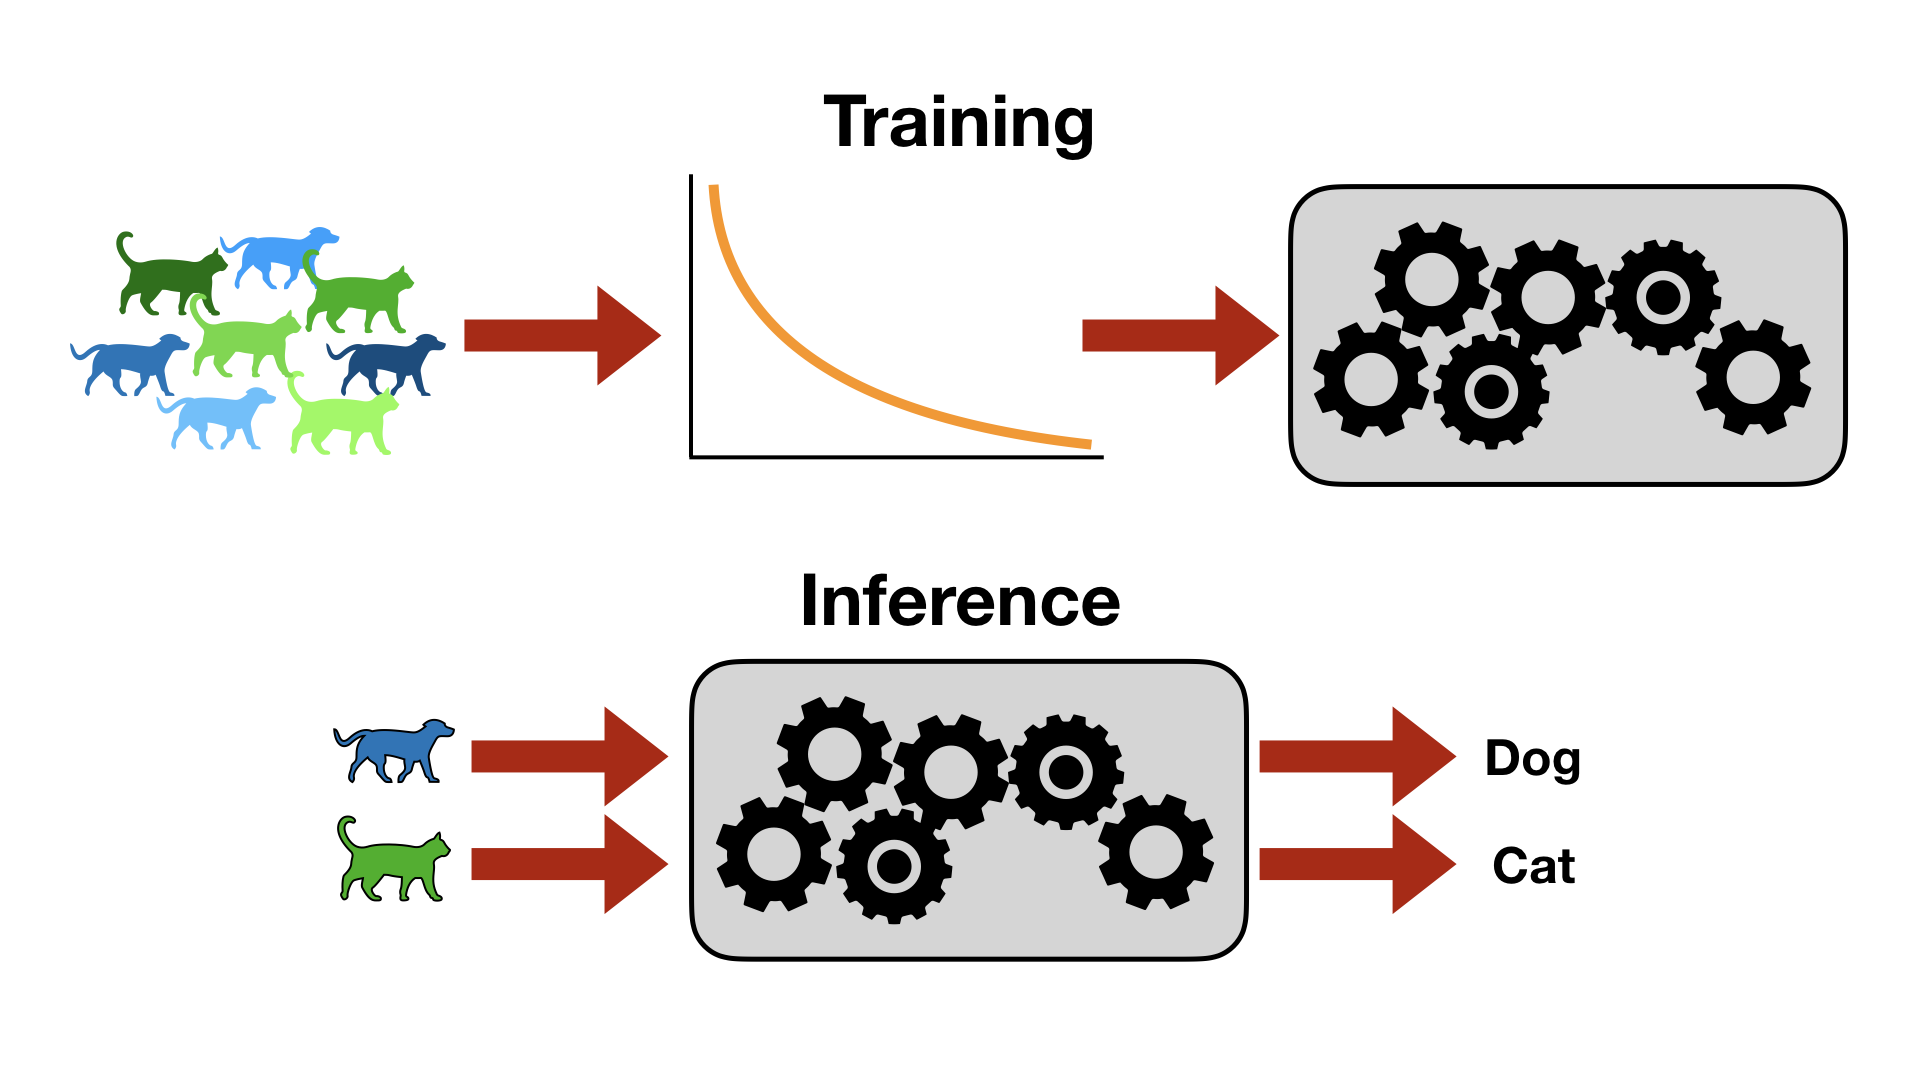
\includegraphics[trim={0 3cm 0 3cm},clip,width=0.95\textwidth]{diss/1_intro/figs/dl.png}
%     \caption[Modern machine learning pipelines]{Machine learning training and inference visualization.}
%     \label{fig:dl}
% \end{figure}
Say we have some dataset comprising of sample pairs $(x,y)$, where we wish to predict $y$ from $x$.
Our prediction, say $\hat{y}$, might be the output of some unknown function $f$ that we attempt to learn from training data. 
Let our approximation to this function be $\hat{y}:=\hat{f}(x)$.
This can take many forms, 
based on assumptions and prior information we may have on the relationships among the data. 
Consider the simple \textit{linear} case,
where we want to learn some parameter $w$ such that $y = w\cdot x$. 
Given $n$ sample pairs $(x_i,y_i)$ indexed by $i$, traditional statistics and optimization literature yield the following \textit{least squares} problem formulation, where we want to minimize the ``squared error'' between the observed values $y_i$ and the predicted $\hat{y}_i:= w\cdot x_i$:
\begin{align}\label{eq:lq}
\hat{f}:=\hat{w} = \mathop{\arg\min}_{w} \sum_{i=1}^n (y_i - w\cdot x_i)^2
\end{align}
This formulation expands without much change to a multi-dimensional form of the input $x$ and respectively, $w$: the canonical case where a number of features, or \textit{covariates} (e.g., symptoms), are used together to predict the outcome (e.g., diagnosis). 
If we are interested in which features of $x$ are important, we can look at the relative values of the learned ``weights'' $w$. In this simple setting, the importance of a feature (say $x^j$) can be exactly determined by the importance of the parameter ($w^j$).
A weight value far from zero may indicate that corresponding feature is important for diagnosis.
% If instead we are interested in which samples are most important, we can use existing methods for sample reweighting or methods that use standard assumptions to efficiently identify important subsets.

In this case and others, traditional statistical learning methods 
have been studied 
for many decades.
Linear regressors, decision trees, and support vector machines
have all been analyzed under these lenses.
% ,
% and as the modern machine learning community
% has returned to these questions recently,
% so has a renewed interest in their methods of analysis.
New research focuses
particularly on the differences
associated with moving from classical \textit{under-parametrized} models to
modern (deep) \textbf{over-parameterized} models: where
the model size vastly outnumbers the number
of input samples.
% , and may even be comparable to 
% the \textit{entire sample space.}
Methods for estimating the number of samples needed,
the time to learn a particular task,
and the generalization ability 
all require new perspectives in this regime.
While nascent, this research
attempts to fill the gap between
statistical and deep models to enable similar measures of sample influence, feature importance, and model understanding. 

\paragraph{A full picture.}
Let us expand our notation from the example above to consider this more general framing.
Consider a dataset $X:=\{x_i\}_{i=1}^n$ of size $n$ where each data point $x_i$ in the set $X$ is drawn from some underlying distribution over the domain $x_i \sim \cX^d$, 
with domain dimensionality (number of features) $d$.
A model $f$ is fit using a parametrization $\theta \in \Theta$,
with $\Theta$ the space of possible parametrizations (models) with some intrinsic dimension $p$. 
%While all three of these problems are closely related, they require different approaches. 
Generalizing the least squares``error measure'' from Eq.~\eqref{eq:lq} to an arbitrary \textit{loss} $\ell$, we have
\begin{align}\label{eq:learning}
    \hat{f}:=\hat{\theta} = \mathop{\arg\min}_{\theta\in\Theta} \sum_{x \in X} \ell(f_\theta(x_i))
\end{align}
From an analysis perspective, 
we might be interested in any one of 
(a) subsets of input features $\cC \subseteq \cX$ that are important for the downstream task,
(b) associating model subsets $\cP \subseteq \Theta$ with specific inputs or groups of inputs, or 
(c) subsets or subgroups of samples $S \subseteq \{X\}$ that are sufficient or representative of the entire dataset.

Crucially, an uninformed search for a subset is computationally infeasible. For a superset of size $n=|X|$, The set of all subsets is the power set, with a size of $2^{n}$! If an identification procedure requires looking over all of these and choosing a ``best'' one by some metric, the procedure will be limited to very small supersets.
Efficient methods have been developed in each of the three contexts above to avoid this exponential search.

\begin{figure}
    \centering
    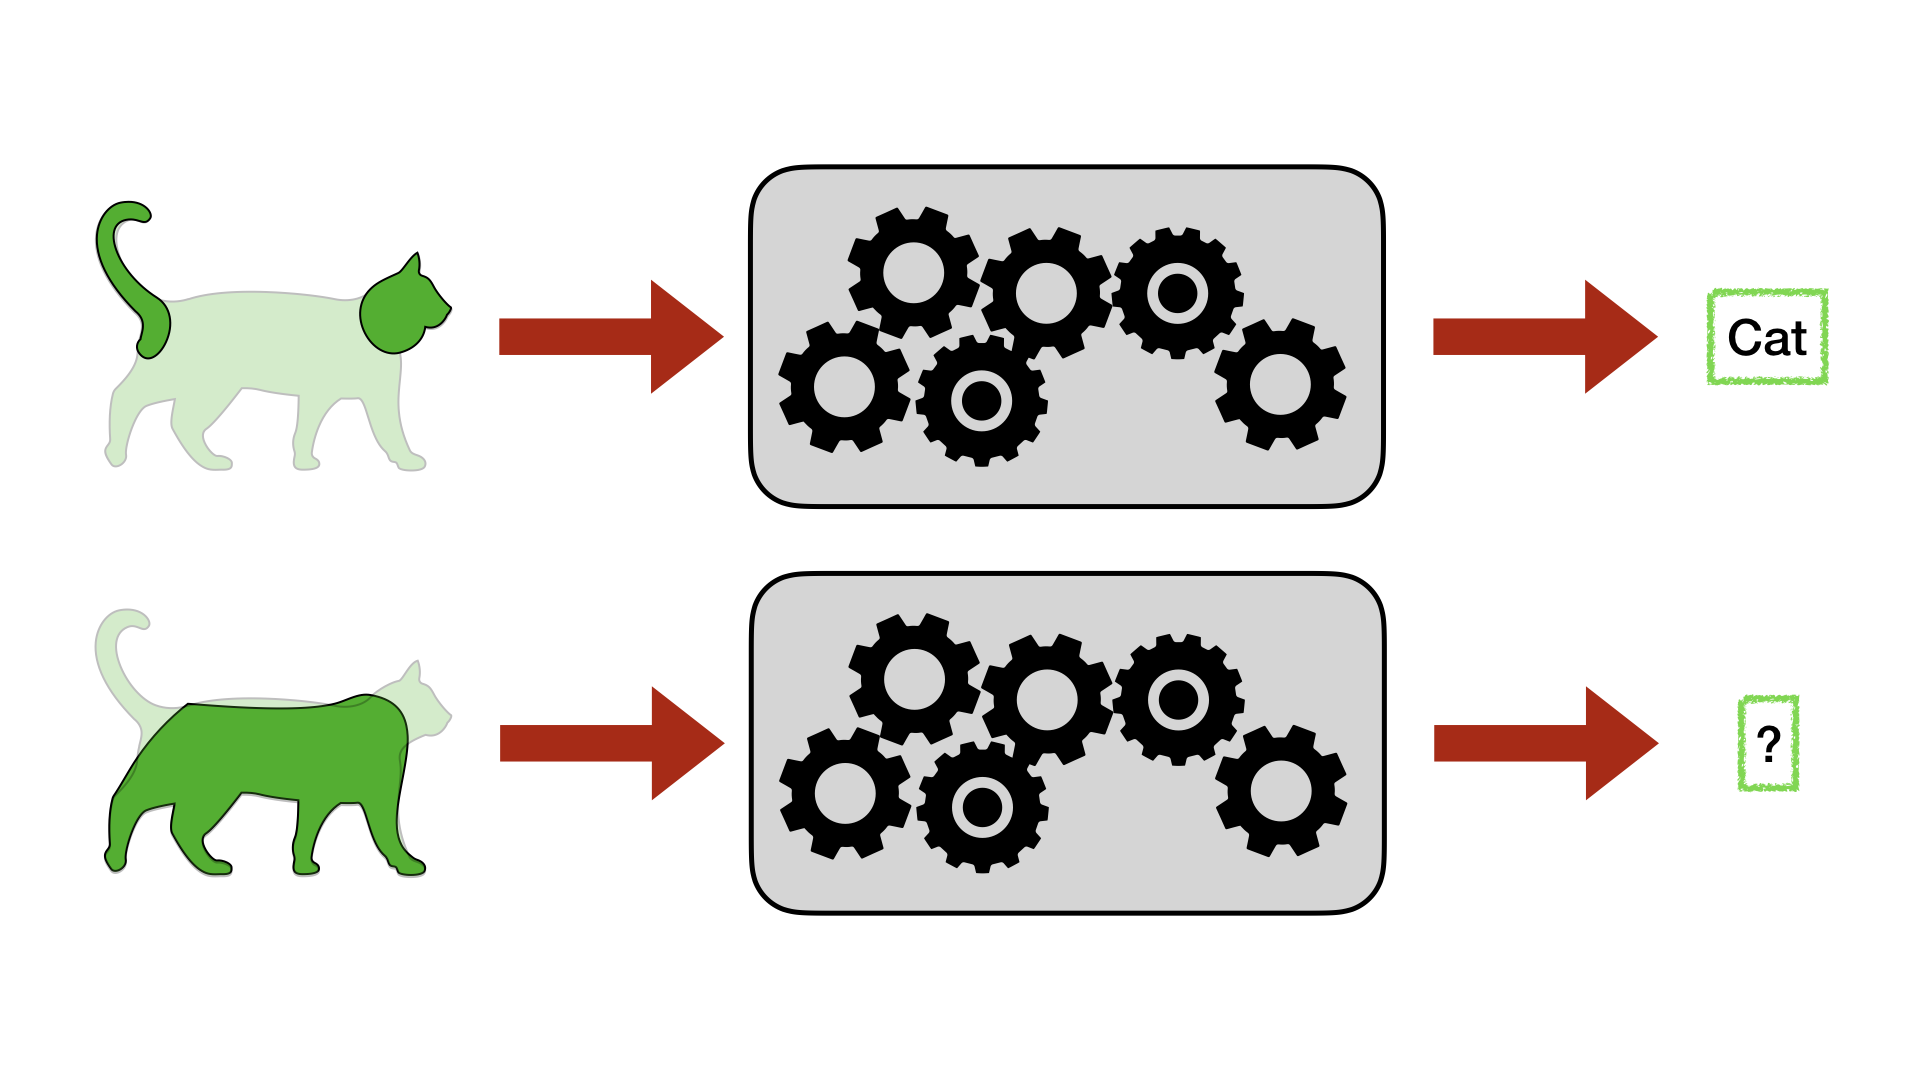
\includegraphics[trim={0 3cm 0 3cm},clip,width=0.9\textwidth]{diss/1_intro/figs/feat_select.png}
    \caption[Visualization of feature selection]{An example of identifying specific features important to the learning task.}
    \label{fig:feat_select}
\end{figure}
\paragraph{Feature Selection.} 
With more complex models $f$ compared to the linear case above, newer ``black-box'' methods have been developed for identifying important features. From the more pure statistics side, scan statistics~\citep{scanstat,scanstatlrt} allow for a structured ``scanning'' over the input space, skipping subsets unlikely to provide additional information for the measure of interest.
Further on the deep learning side, adaptations of sensitivity analysis, via noise addition and perturbations have found success~\citep{yeung2010sensitivity,zhang2015sensitivity}, alongside activation mapping~\citep{cam,selvaraju2017grad}.
These methods typically generate an analagous ``weighting'' over the input space, identifying features most salient for the specific task (Figure~\ref{fig:feat_select}).

\begin{figure}
    \centering
    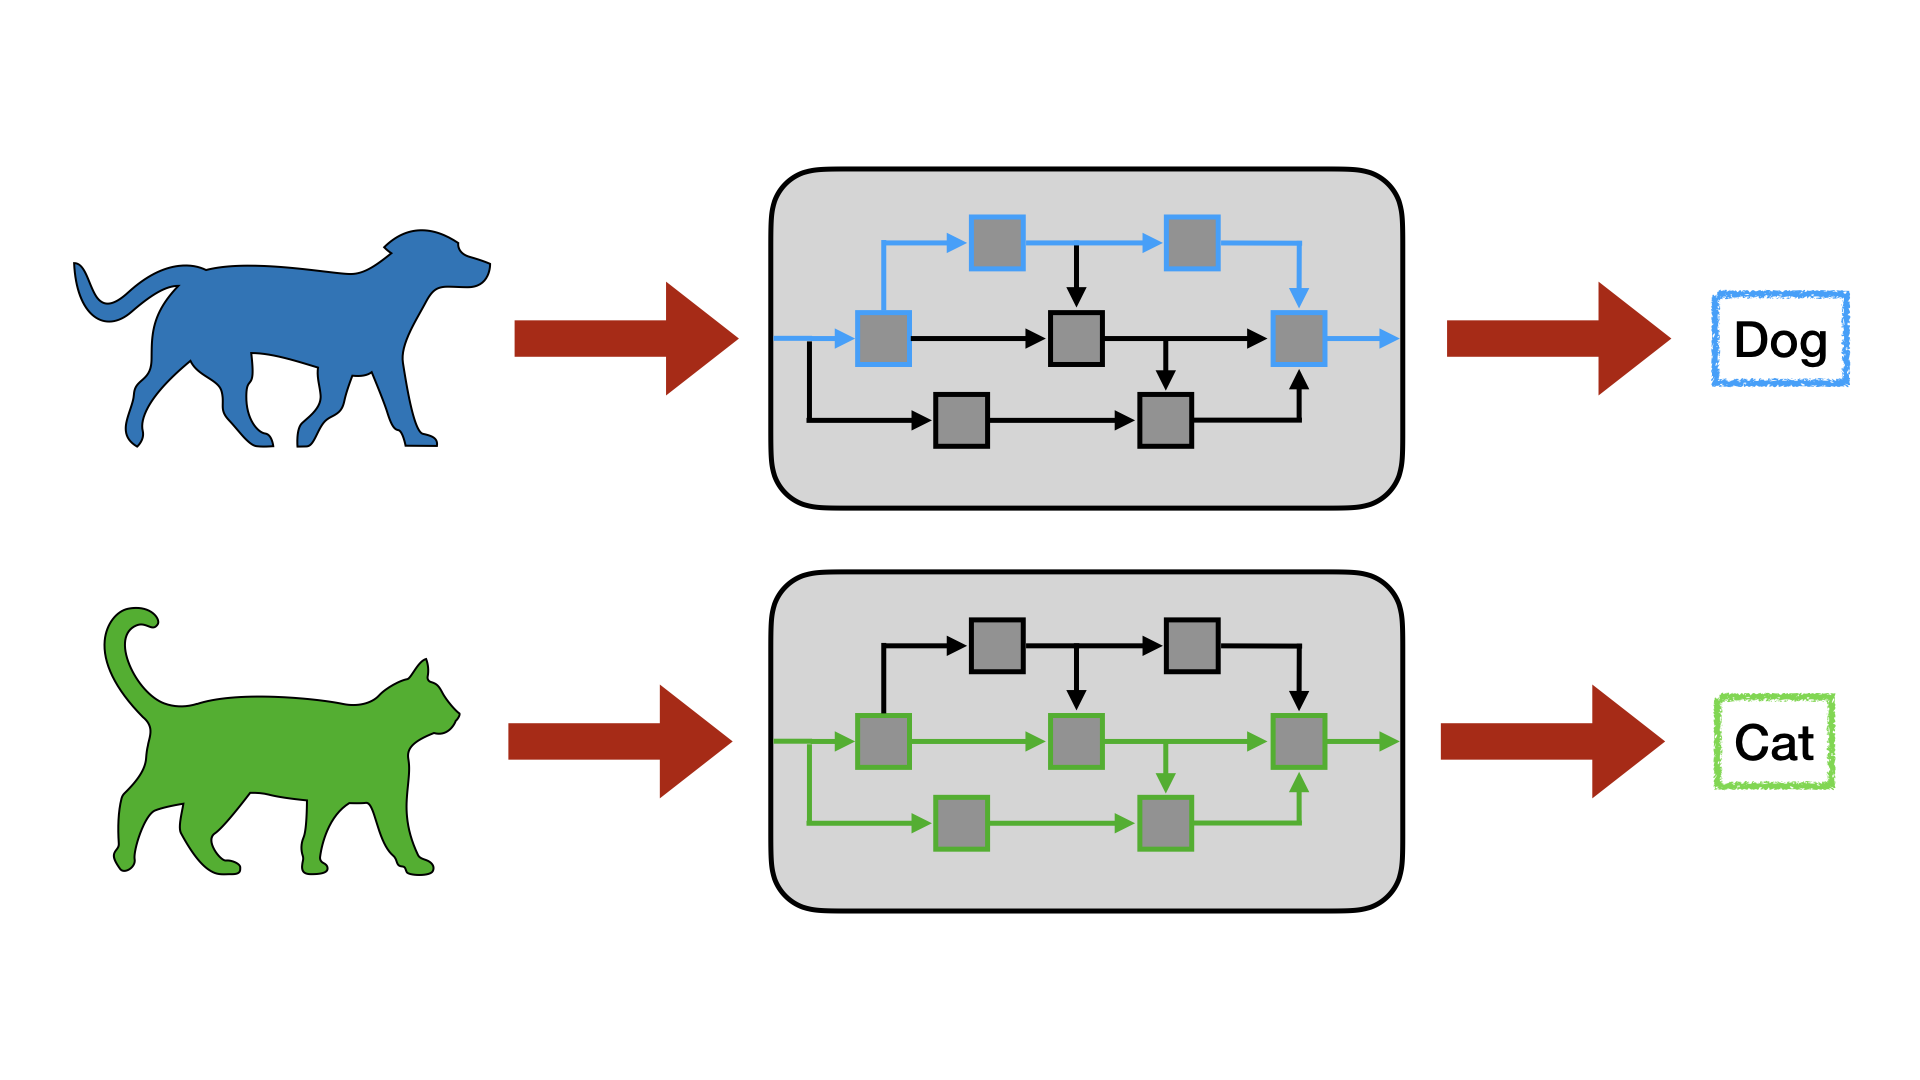
\includegraphics[trim={0 3cm 0 3cm},clip,width=0.9\textwidth]{diss/1_intro/figs/param_select.png}
    \caption[Visualization of parameter selection]{An example of identifying specific parameters important to the learning task.}
    \label{fig:param_select}
\end{figure}
\paragraph{Parameter Selection.} 
Selection in the model space generally takes two forms. First, as a prior, restriction, or assumption over the model space, and second, as a post-hoc method for an ``explainable'' proxy.
Regularization, sparsity, and gating methods are often used independent of the type or size of the model, to encourage the solution to fall within a specific region of the model space.
% In non-deep settings these methods come with strong theoretical guarantees. 
The theoretical underpinnings of these methods in deep learning are still being actively researched~\citep{hardt2016train,jacot2018neural,neyshabur2014search}, but the methods have nonetheless been effective in practice. 
On the post-hoc side, of particular interest are the parameters relevant to specific regions of the input space \textit{after} training (Figure~\ref{fig:param_select}). Here, recent analysis of deployed networks has shown this to be true~\citep{bau2017network,fong2018net2vec}, and current work continues to explore these network regions to aid in interpretability and explainability.

\paragraph{Sample Selection.} Many methods have been developed for outlier detection within training or testing sets~\citep{huang2020feature,ren2019likelihood} \textit{after} training, as well as methods for understanding sample influence~\citep{koh2017understanding,golatkar2020eternal,huang2020feature} . ``In-the-loop'' methods for accounting for ``outlierness'' behave similarly to accounting for group or individual fairness while training~\cite{mehrabi2021survey}. Unfortunately, once samples are identified in some manner, post-hoc adjustments to a trained model are generally very difficult. Recent work has focused on ``unlearning'', or removing a sample's influence on a model without retraining. If specific samples can be uniquely identified, performance and privacy reasons may require these specific interventions to reduce the ``influence'' of that sample subset.
\begin{figure}
    \centering
    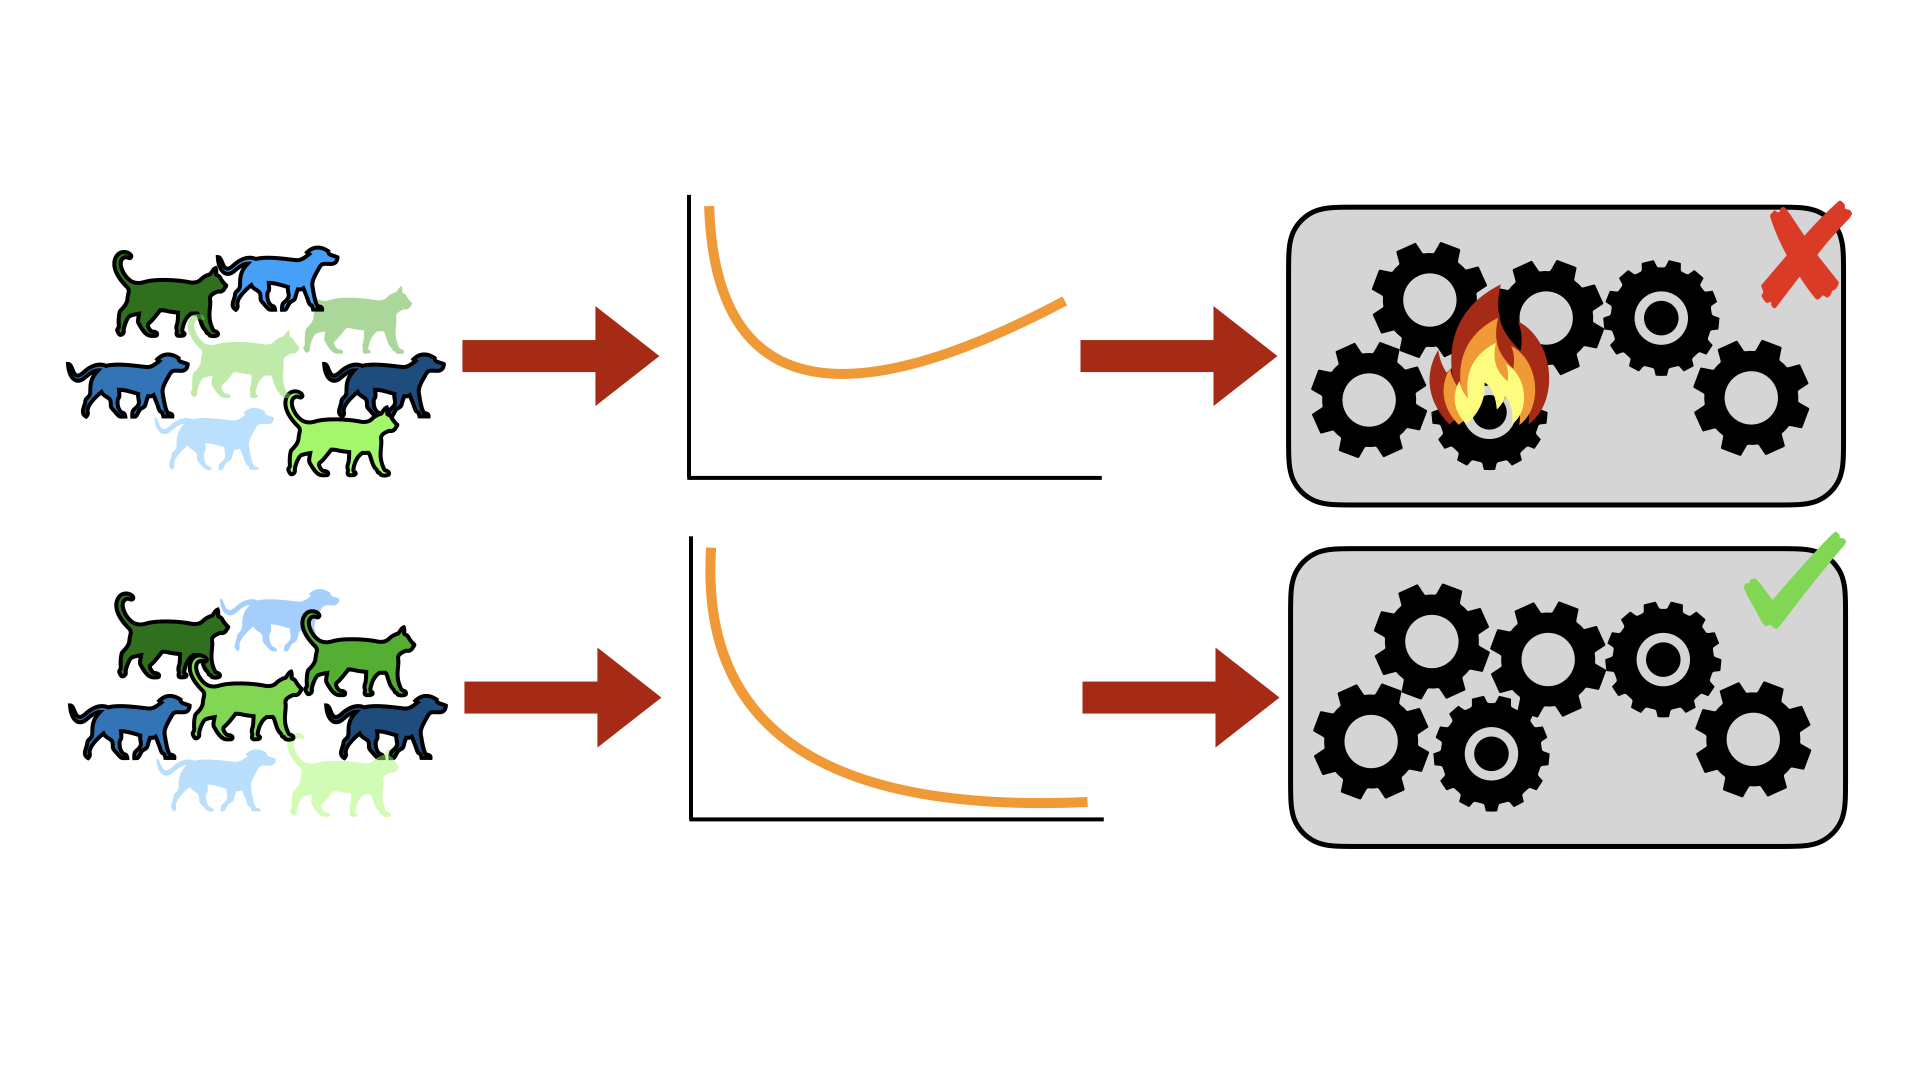
\includegraphics[trim={0 4.5cm 0 4cm},clip,width=0.9\textwidth]{diss/1_intro/figs/sample_select.png}
    \caption[Visualization of sample selection]{An example of identifying specific samples important to the learning task.}
    \label{fig:sample_select}
\end{figure}


\begin{mdframed}[style=MyFrame]
\textbf{ Thesis Goal: }
\em Identify, construct, and evaluate methods for \textbf{efficient} subset identification in modern machine learning feature, model, and input spaces.
\end{mdframed}

\section{A Few Motivating Examples}
Consider a traditional machine learning classification task in which we would like to predict whether an individual has a specific disease condition based on a medical resonance image (MRI) scan of their brain. Our input feature $x$ may consist of a 3D-array of values in $\RR^{\cI\times \cJ\times \cK}$ measuring some intensity of the imaging modality at each voxel, indexed by a tuple $(i,j,k) \in (\cI,\cJ,\cK)$.
Our outcome variable $y$ may simply be a binary label of whether the input scan has been labeled by a radiologist as one demonstrating typical disease characteristics.
Using an off the shelf 3D convolutional neural network with adjustments to match our input size, we can very quickly set up and train a system to predict disease presence with a high degree of accuracy.

\paragraph{Example 1.}
With a prediction for a specific scan, or predictions over a number of scans, we might be interested in identifying which regions of the brain are most important for diagnosis. These regions, $R \subset \cR:=\RR^{x\times y\times z}$, can be specific groups of pixels in the image that may correspond to known functional networks. Methods such as attention and class activation maps may work here, but there are a few issues. The number of samples available to learn a model is very small compared to the both the dimension of the input and the number of parameters in the model, i.e., $n \ll p$ and $n \ll d$. Thus it is very easy to overfit, and for areas of interest to be associated with intricacies of particular input data rather than true, real differences defined by the disease.

Furthermore, recent medical imaging studies have moved past simple difference detection: trends over time, and the ability to predict {\em future} disease development have by far become the setting of most interest.
Given an image of a healthy individual, is it possible to predict what their scan, or their future disease diagnosis, may be up to 10, 20, or more years in the future?
If a number of scans have been collected over some timeframe, can the \textit{trajectory} of the individuals' development be extrapolated to estimate progression?
As traditional models extended for temporal analysis grow in both size and complexity,
a number of subproblems explicitly related to model and input subspaces arise. In this thesis we address two such problems: \textbf{statistically rigorous identification of temporally evolving subsets}, and \textbf{characterizations of deep models that enable efficient training of recurrent models with large scale time-varying data}.
    
\paragraph{Example 2.}
With the rapid growth of AI and machine learning applications has come valid concerns regarding both guarantees of privacy.
Recent technology legislation has made the importance clear in all aspects of data use,
and particular projects and groups have demonstrated that machine learning is not independent of
this need \citep{Exposing}.
A new issue raised within this intersection is the ``right to be forgotten".
If a model has been trained with a particular users' data, 
they should have some recourse or right
to both remove their data from the training set,
and also know that the model has not learned from their data.
On the surface, this poses a significant problem for model builders
and organizations that spend large amounts
of time and resources in 
training deep learning models.

In the medical imaging example above this is especially important: with fewer samples it is more likely that information about any particular one could ``leak'', and the model's performance may degrade significantly as a relatively large percentage of it's training data is removed.
Thus tailored methods must be developed to ensure both privacy and performance, without requiring full retraining.
As we will see, 
\textbf{identification of model parameter subsets}
that are particularly important
for a particular sample's influence
in a model enables \textit{efficient machine unlearning}.

\paragraph{Example 3.}
From an alternative perspective, we may want to identify specific samples rather than have them specified a priori.
Traditionally a rigorous area of study under classical statistics, outlier detection and accounting have become a subfocus for many within the machine learning community as well \citep{golatkar2020eternal,golatkar2020forgetting,huang2020feature,ren2019likelihood}.
While subgroups of input samples may be outliers, it is more often the case that they represent known heterogeneity within the data. 
These differences may be marked using 
group information known a priori, and 
most learning tasks aim to learn tasks
in a \textit{subgroup-independent} manner.
In our disease prediction model above,
these groups could simply be stratified by the type of scanner used to acquire the image, but it could also
be a systematic difference correlated with some protected attribute. {\color{red} sentence about original brain atlas for registration being eurocentric}
This can directly lead to disparate performance and results on \textit{all} individuals outside of that group.
Optimization and regularization methods with this focus come under the umbrella of model fairness.
However, many existing methods do not scale well to larger models or as the number of subgroups grows, as is often the case when intersections of protected classes must be considered. Here we identify and construct a particular solution for \textbf{groupwise fairness that enables efficient in the loop fairness regularization}.

% What features are most important for prediction?
% Which samples were most important for my training?
% Can we understand when a model is certain or uncertain about its output?
% Are there layers in my network that have learned a particular subtask?
% Questions of robustness, bias, influence, fairness, and importance have become central questions to contemporary machine learning research \citep{doshi2017towards,mehrabi2021survey,amodei2016concrete}.
% machine learning, etc.

% Feature selection in the case of
% typical regression or classification 
% takes some form of learning parameters $\theta$ that allow for $\hat{y} = f_\theta(x)$ to be close to the true outcome of interest $y$.
% While forms of data $X := (x,y)$ may simply be continuous and real-valued, modern machine learning has greatly expanded formulations of the classical learning problem to include a wide variety of structured learning problems~\citep{nowozin2011structured}. 
% Consider the case when a high-dimensional input is used to predict an output with a highly-parametrized model. 
% Once learned, obvious questions arise as discussed above: are there specific low-dimensional spaces in either the input or the model space that are most important or necessary for the global learning problem of interest? Are there specific subspaces associated with particular subproblems of the global problem?
% The machine learning literature has come up with a number of ways to identify analogs of these spaces, 
% including extensions of sensitivity analysis to deep learning~\citep{yeung2010sensitivity,zhang2015sensitivity}, and constructing and identifying nonzero model subsets via particular model choices such as activations~\citep{selvaraju2017grad} and regularizers.
% In classical settings these are well understood: decision trees naturally provide ease of interpretibility via the information used to choose splits, and both linear and kernel support vector machines have been analyzed to provide for measures of sample importance via distances to the margin as well as feature importance via weights defining the learned hyperplane~\citep{Mitchell97}.
% Attention and saliency maps have emerged as popular new methods,
% given their ease of implementation and interpretation~\citep{sutskever2014sequence,vaswani2017attention,selvaraju2017grad}.
% By learning dimensions of a given input that are particularly important, either in a hard (binary) or soft (continuous weighting) manner, model builders are better able to understand and interpret what a model has learnt.
% The specific ideas of attention notwithstanding, many of these existing methods are far removed from traditional hypothesis testing frameworks.
% While some work has begun in this direction~\citep{tansey2018black},
% there remains a gap in direct identification of subsets and structures in these spaces that can be defined in statistically rigorous manners.

% \begin{figure}
%     \centering
%     \includegraphics[width=0.5\textwidth]{example-image-a}
%     \caption[A simple subset selection example]{\color{red} Identifying and selecting in MRIs, subset, sample, model ID.}
% \end{figure}

% \paragraph{A specific example.} 

% ------------------------------------------

% below here will be moved and arranged with the "selection" sections and here if relevant

% ------------------------------------------

% While attention can be directly applied to the network in order to identify ``hotspots" in the input space relating to the learned classification task, 
% given the high-dimensional nature of the input
% and the relatively small sample size 
% associated with medical imaging data, 
% it is very likely that an area of interest identified
% may be an intricacy of the training samples used rather than truly a region of disease signal.
% Class activation maps (CAMs) may be unclear, and can often associate with image artifacts unrelated to the scientific task~\citep{adebayo2018sanity}.
% Methods of generalization may help to increase confidence in identified regions, but statistical guarantees often remain out of reach.

% Furthermore, most recent problems associated with medical data have moved past simple difference detection: trends over time, and the ability to predict {\em future} disease development has by far become the setting of most interest.
% Given an image of a healthy individual, is it possible to predict what their scan, or their future disease diagnosis, may be up to 10, 20, or more years in the future?
% If a number of scans have been collected over some timeframe, can the \textit{trajectory} of the individuals' development be extrapolated to estimate progression?
% As traditional models extended for temporal analysis grow in both size and complexity,
% a number of subproblems explicitly related to model and input subspaces arise. Here we address two such problems: \textbf{statistically rigorous identification of temporally evolving subsets}, and \textbf{characterizations of deep models that enable efficient training of recurrent models with large scale time-varying data}.

% A sample's particular influence on model parameters aside, the identification of influential samples or subsets of samples more generally is of independent interest. 
% Traditionally a rigorous area of study under classical statistics, outlier detection and accounting have become a subfocus for many within the machine learning community as well \citep{golatkar2020eternal,golatkar2020forgetting,huang2020feature,ren2019likelihood}.
% While subgroups of input samples may be outliers, it is more often the case that they represent known heterogeneity within the data. 
% These differences are typically marked using 
% group information known a priori, and 
% most learning tasks aim to learn tasks
% in a \textit{subgroup-independent} manner.
% Optimization and regularization methods with this focus come under the umbrella of model fairness, and instead of identifying and boosting independences within the model or data, we aim to minimize them.
% However, many existing methods do not scale well as the number of subgroups grows, as is often the case when intersections of protected classes must be considered. In the sequel we identify and construct a particular solution for \textbf{groupwise fairness that enables efficient in the loop fairness regularization}.

\begin{mdframed}[style=MyFrame]
\em 
Here we focus our effort on identifying these important subsets of model, feature, and sample space for feature association, model size reduction, model unlearning, and, fairness. Specifically, taking advantage of both existing statistical and geometric methods, we develop new methods for localizing subsets in a range of settings from hypothesis testing to deep learning.
\end{mdframed}

\section{Thesis Scope and Contributions}

We explore the intersections of classical statistical and geometric constructions with modern machine learning methods. 
Figure~\ref{fig:scope} shows the overall scope projected along three axes: feature, parameter, and sample spaces.
Below we briefly introduce the main problems studied in this thesis.
\begin{figure}[!ht]
    \centering
    % \includegraphics[width=0.99\linewidth]{scope.pdf}
    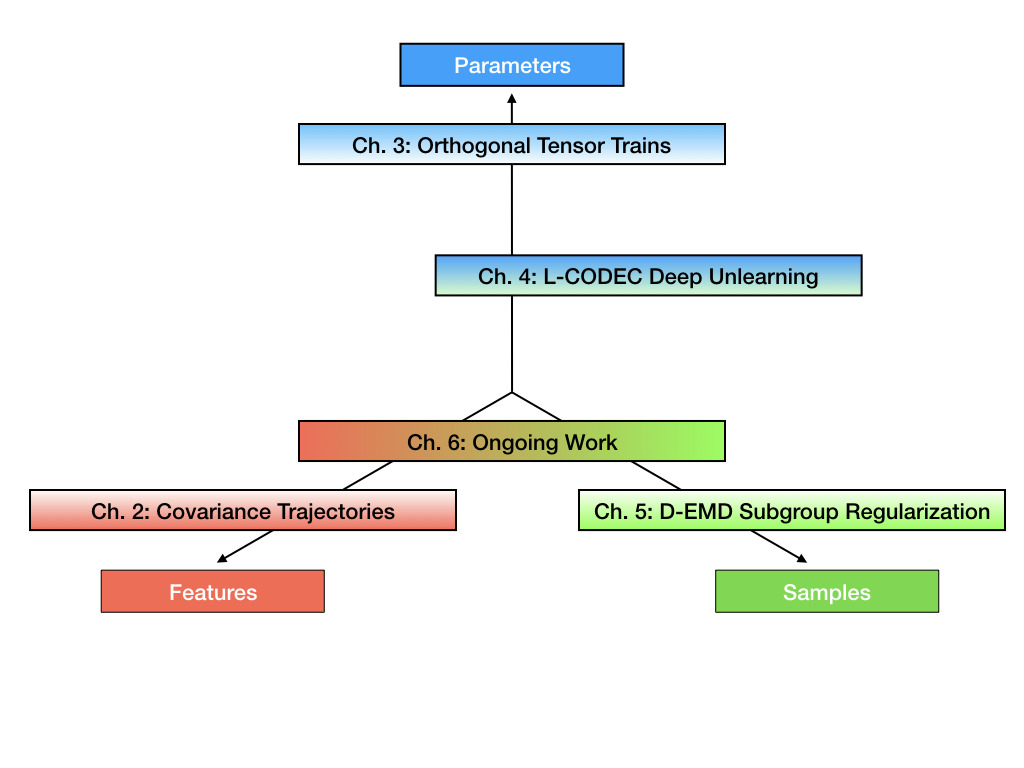
\includegraphics[width=0.95\linewidth]{diss/1_intro/figs/thesis_scope.png}
    \caption[Thesis Scope]{Thesis scope, projected over three representative axes. {\color{red} update chapter numbers shift by 1}}
    \label{fig:scope}
\end{figure}

\subsection{Second-Order Modeling and Group Difference Analysis over Time}

Recent results in coupled or temporal graphical models offer schemes for estimating the relationship structure 
between features when the data come from
related (but distinct) longitudinal sources. A novel application of these ideas is for analyzing group-level differences, i.e., in identifying if {\em trends} of estimated objects (e.g., 
covariance or precision matrices) are different across disparate conditions (e.g., gender or disease). Often, poor effect sizes make detecting the \textit{differential} signal 
over the {\em full} set of features difficult: for example, 
dependencies between only a {\em subset of features} may manifest differently across groups.
We first suggest
a parametric model 
for estimating trends in the space of $\SPD$ matrices as a function of one or more covariates.
We will then generalize scan statistics to graph structures, 
to search over distinct subsets of features (graph partitions) whose temporal dependency structure may show statistically 
significant group-wise differences.
We will theoretically analyze the Family Wise Error Rate (FWER) and bounds on Type 1 and Type 2 error. 
On a cohort of individuals with risk factors for Alzheimer's disease (but otherwise cognitively healthy), 
we 
find scientifically interesting 
group differences where the default analysis, 
i.e., models estimated on the full set of features, do not survive reasonable 
significance thresholds. 
% Preliminary work on this was published in \citep{covtraj}.


\subsection{Efficient Tensor Representations for Feasible Temporal Deep Learning}

Modern deep networks have proven to be very effective for analyzing real world images.
However, their application in medical imaging is still in its early stages,
primarily due to the large dimension of three-dimensional images, requiring enormous convolutional or fully connected layers --
if we treat an image (and not image patches) as a sample. 
These issues only compound when the focus moves towards longitudinal analysis
through recurrent structures, and when a point estimate of model parameters is insufficient 
in scientific applications where a reliability measure is necessary.
Using insights from differential geometry, 
we will adapt 
the tensor train decomposition to construct networks
with significantly fewer parameters,
allowing us to train powerful recurrent networks on whole brain image volumes. 
We analyze 
the \textit{orthogonal tensor train},
and demonstrate its ability to express a standard network layer both theoretically and empirically.
We 
demonstrate its ability to 
effectively reconstruct whole brain volumes
with faster convergence and stronger confidence intervals
compared to the standard tensor train decomposition. 
We provide code and show experiments on the ADNI dataset
using image sequences to regress on a cognition related outcome.
% Preliminary work on this was published in \citep{ott}.

\subsection{Practical Unlearning via Large-Scale Conditional Independence Testing}

%With AI systems extensively using personal %data for model training, 
Recent legislation has
led to interest in {\em machine unlearning}, i.e., removing specific training samples from a {\em predictive} model as if they never existed in the training dataset. 
Unlearning may also be required due to  corrupted/adversarial data or simply a user's updated privacy requirement.
For models which require no training ($k$-NN), 
simply deleting the closest original sample can be effective. 
%However, it is not clear how such approaches can be used to unlearn 
%models that contain rich information learned from the original data.
But this idea is inapplicable to models which learn richer 
representations.
%from data. 
%Recently, optimization-based unlearning estimators have been proposed, but 5their 
Recent ideas leveraging optimization-based updates
scale poorly with the model dimension $d$,  
due to 
inverting the Hessian of the loss function. %with an overall cost of $O(d^3)$ 
%is prohibitive.
We describe
a variant of a new conditional independence coefficient, 
L-CODEC, to identify a subset of the model parameters with the most semantic overlap on an individual sample level. 
Our approach completely avoids the need to invert a (possibly) huge matrix. 
By utilizing a Markov blanket selection, 
we find
that L-CODEC is also suitable for deep unlearning,
as well as other applications in vision.
Compared to alternatives, L-CODEC makes approximate unlearning possible 
in settings that would otherwise be infeasible, 
including vision models used for face recognition, 
person re-identification 
and NLP models that may require unlearning samples identified for exclusion.
% Preliminary work on this will appear in \citep{lcodec}.


\subsection{Reducing Subgroup Fairness via High Dimensional Earth Mover's Distances}

Optimal transport has recently emerged as a useful tool for machine learning through its connections with geometry, statistical machine learning, and through practical algorithms. Existing methods that leverage optimal transport often  regularize using  a Wasserstein metric or by computing barycenters, for example. %which are effective when distributions are continuous and known, or when measures of interest are discrete.
% Our formulation allows for a discretization of continuous measures that drop in directly to classical  formulations of the Earth Mover's Distance. 
We leverage optimal transport, except that we take advantage of a recently-introduced algorithm that computes a generalized earth mover's distance.
Not only is this algorithm computationally cheaper to compute compared to existing barycentric measures, but our method has the additional  advantage that gradients used for backpropagation can be directly read off of the forward pass computation, which leads to substantially faster model training.
We provide technical details about this new regularization term and its properties, 
and 
experimental demonstrations of improved training speed over existing Wasserstein-style methods.

{\color{red}
\subsection{Understanding Latent Spaces via Conditional Independences}

The final chapter of this thesis applies some of the tools developed above in the analysis of latent spaces in recent large scale models.
% In these studies, 
% we aim to identify conditionally independent features and subjects that are particularly important to the prediction and estimation of
% key disease outcomes,
% as a function of a number 
% of demographic, neuropsychological,
% genetic,
% and imaging data collected as 
% part of an ongoing consortium 
% to understand the progression
% of Alzheimer's disease in younger, 
% asymptomatic populations.
% In what follows we present
% exploratory analysis
% on a small, easily 
% digestible subset of the available data,
% that lays the foundation for
% further analysis.
}
% This work is the most forward looking, and aims to be a stepping stone toward a rigorous 

\section{Outline}
Chapter 2 covers the essential background necessary for the developments presented in the following chapters, including specifics of graphs and hypothesis testing, as well as relevant modern methods for learning and optimization.
In Chapters 3 through 7, we describe four perspectives to address subset identification.
Chapter 3 explores and focuses on the identification of feature subsets varying over time.
In Chapter 4 we describe a method of constraining the parameter space in a particular manner
that enables more efficient large scale neural networks.
Next, Chapter 5 provides a solution to the machine unlearning problem,
enabled through a particular conditional independence parameter selection scheme, vastly reducing network update costs.
Chapter 6 ends with a unique solution to subgroup fairness, 
where we take advantage of an efficient solution to
the $d$-dimensional earth mover's problem
to regularize large models when the number of subgroups can be large.
{\color{red} Chapter 7 describes future work, focused on applying a particular solution from Chapter 5 to understanding relationships among features in latent spaces learned by large generative models.}


%%%%%%%%%%%%% 
% Some old stuff

% Significant progress in the modern development of machine learning has
% been built upon connections and patterns identified across myriad
% interdisciplinary fields of study.
% Up through the mid 2000's, 
% many of these methods were inspired by and interested in 
% highly focused and constrained problems. 
% With a reasonably sized input domain, could a model of roughly equal size be used to
% predict some output?
% Linear regressors, decision trees, and support vector machines were all answers to these questions, with their own
% varying degrees of scaling and complexity.
% These methods necessitated carefully constructed formulations with specific restrictions to the learnable function class,
% enabling straightforward analysis 
% for provable performance guarantees 
% and easy identification of critical training samples and important input features.

% Contemporary machine learning, however, has a vastly different modus operandi. 
% Driven in large part by the exponential growth of available computation via Moore's Law, \textit{deep learning} has fallen squarely in the realm of \textbf{over-parameterized} models.
% With these overparametrizations and computation capacity, the typical learning questions posed as maximizing accuracy or reducing error have largely been addressed for even large scale problems.
% As such, complementary questions have led to subfields focusing on other performance measures, such as robustness, fairness, interpretability, and explainability.
% Many solutions to these questions end up looking back at answers found for the under- or non-parametrized settings.
% While nascent, these approaches 
% attempt to fill the gap between
% statistical and deep models to enable similar measures of sample influence, feature importance, and model analysis. 
% Most notable amongst these newer approaches is that of (Self)-Attention in Neural Networks \citep{sutskever2014sequence,vaswani2017attention}.
% Other proposals 
% end up looking back at the types of analysis typical of those more classical under-parametrized or nonparametrized methods.

% Not limited to previous developments in learning or computation theory, the arguably most valuable contributions toward the exponential reduction in model error can be attributed to influences and intuitions taken
% from biology, psychology, neuroscience, and even XXX \citep{srivastava, etc}.
% Perhaps one explanation as to why this phenomenon exists may be attributed to the way in which deep learning evolved. 
% The classical learning goal of function approximation lends itself nicely to a system which allows for arbitrary complexity via simple changes (e.g., addition of neural network layers). % Foundational works building on the original neural networks particularly have taken advantage of constraining this space of functions to search over: 
% the most seminal case being those of convolutional filters for imaging data. 
% While ``constraints" of this form have helped tremendously in model performance on modern vision and language machine learning tasks (GANs, Recurrent Networks, Residual Layers, Transformers, etc.), the ability to identify \textit{subsets} of important samples, input features, and model parameters has lagged significantly behind the development of these methods.
% Recently larger interest has been taken by the community to understand and interpret models with this view, only after extremely large and opaque models have become ubiquitous.
%This lag directly explains the more recent interest in developing methods for understanding and interpreting large scale machine learning models.
\chapter{Introduction} \label{chap:intro} 

Modern applications of machine learning in a broad range of industrial and consumer-facing systems have become ubiquitous.
Most interactions with daily technologies now intrinsically involve 
a request to some ``smart`` system in the ``cloud'', 
where those interactions range from
a request for map directions 
to simply loading a webpage.
Neural network models, and the recent advances of deep learning,
have enabled these systems that 
make such applications possible.
These models have achieved
human-level performance on learning tasks
including image classification~\citep{resnet,alexnet}, image segmentation~\citep{segmentation}, video analysis~\citep{zhang2016video}, text understanding and generation~\citep{bert,gpt}, and have slowly begun to solve more fundamental scientific problems such as protein folding~\citep{protein} drug discovery~\citep{drugdisc}, and medical diagnosis~\citep{diag}.
While this performance is largely attributed to model size,
the abundance of high quality training data
has equally contributed to real world performance,
enabling model training over millions of real world samples~\citep{imagenet,laion},
and potentially billions of synthetic samples via environment simulation~\citep{mcts}.

While deployment in some domains (recommender systems, object detection) may benefit almost unconditionally from this vastly expanded capability, rightful hesitancy has limited their widespread use in particular applications where impacts on individuals, people, or environments may be at stake.
These ``last mile'' concerns take a few forms.
% Because a completely accurate model is still out of reach, an important question that needs to be answered is: which inputs or individuals are being given incorrect outcomes, and why?
% maybe a sentence suggesting unlearning/removal
In mission critical applications such as medical diagnosis, 
the impact of an error can be extremely large,
even if a misprediction happens extremely infrequently.
Additionally, large scale model training and architecture search
can require exorbitant amounts of energy producing high emissions,
and their scale can limit market participants
to only large actors with vast existing resources.
The accessibility and effectiveness of these models can also vary significantly based on the training data, and disparate outcomes can be exacerbated by existing social inequity.

While existing human or ``natural'' systems that these models aim to assist are not perfect, 
our real world has developed norms and regulations that 
enable them to function.
A medical diagnosis might require a physician to explain what symptoms led them to that particular conclusion.
Energy metering and carbon taxes may be applied to limit
emissions.
Regulatory satisfaction may require 
analysis proving equal opportunity,
or that specific protected classes
are not used in decision making.
% Specifically, these can include ideas as simple as the Hippocratic Oath and medical malpractice insurance, to asking your doctor what symptoms lead them to a particular diagnosis.
These ideas are difficult to directly translate to automated machine learning systems,
but proxies have been identified that we can build upon.

These norms and regulations answer a number of questions we may also try to pose to our machine learning models.
What is the cost to learn this task?
What led to this particular outcome?
Why is this outcome different from another?
% We will explore how these questions can be formulated concretely. 

If the answer to these questions is negative or unknown,  follow-up questions all take an interesting form:
Can we learn a smaller model with similar performance? 
Can we identify the most important features? 
Which individuals or groups are being treated unfairly, and can we change that?
These questions ask us to identify a \textit{subset} of some relevant set, dependent on setting, and this identification is our focus here.

% Moving specifically to machine learning methods,
Taking a step back, let's take a look at a representative system. Figure~\ref{fig:dl} illustrates a typical learning pipeline. 
A dataset is collected and used to train a model, by minimizing the error over
those samples in the dataset (top).
A ``sample'' can be a single measured value, or it can
be a large, highly structured object with many ``features.''
The model is made up of some ``parameters'' that are 
tuned during training to learn a good predictor over the training dataset.
This model is then used to predict, or \textit{infer}, on new
data seen ``in the wild'' (bottom).
Our questions above are formally asking to identify \textit{subsets of these objects}: is a subset of the model parameters sufficient for learning? Which subset of the features are important for a prediction? Which subset of the dataset exhibit a specific attribute?
\begin{figure}
    \centering
    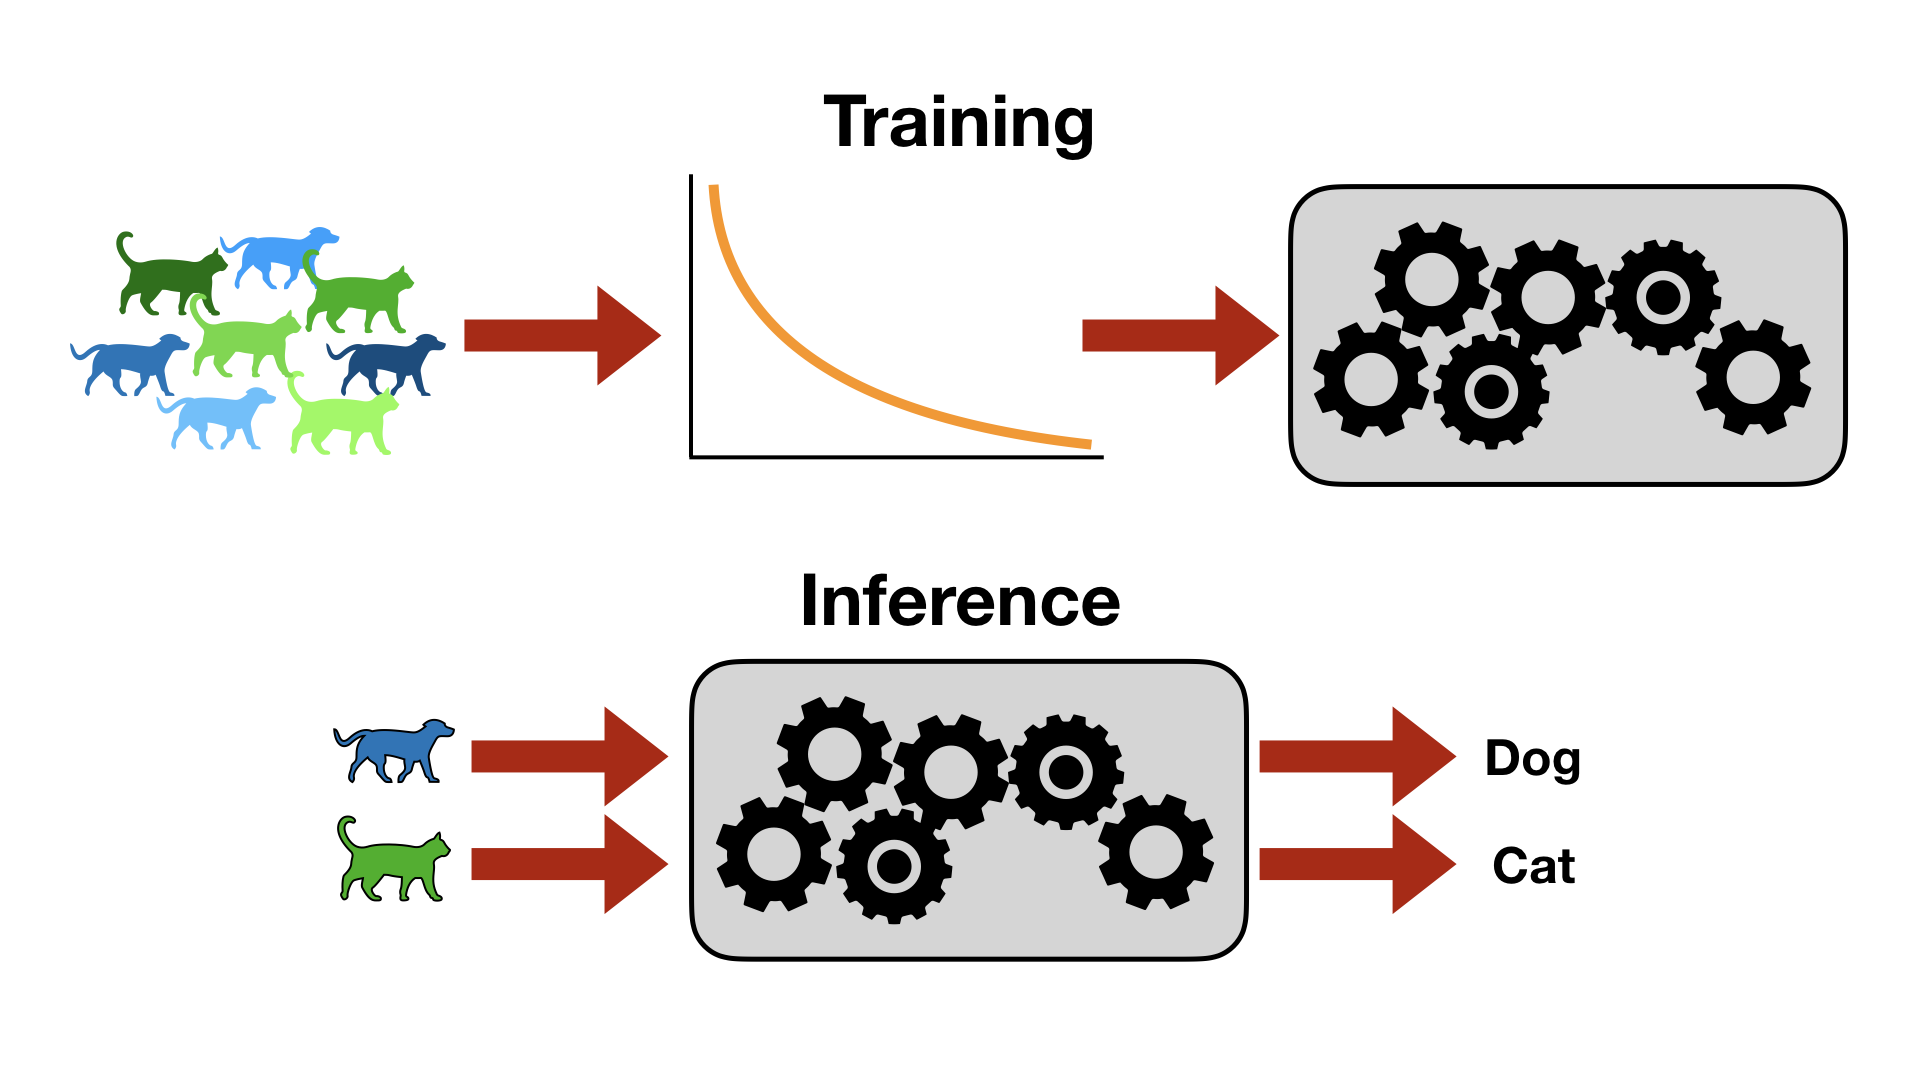
\includegraphics[trim={0 3cm 0 3cm},clip,width=0.95\textwidth]{diss/1_intro/figs/dl.png}
    \caption[Modern machine learning pipelines]{Machine learning training and inference visualization.}
    \label{fig:dl}
\end{figure}

% \textit{Explainability} can be seen as identifying important features of the input, as well as parts of the model (parameters) that ``light up`` for that input. \textit{Fairness} can be evaluated via measures over subsets of the data that correspond to specific groups. 

\begin{mdframed}[style=MyFrame]
\em 
\textbf{This thesis} focuses its main efforts on identifying these important subsets of model, feature, and sample space, to enable answering questions necessary for mainstream adoption of machine learning methods.
\end{mdframed}

% In this dissertation, we explore the sizes of these models, samples, and datasets, and 
% analyze under what situations 
% a smaller \textit{subset} of them may be sufficient or important
% for questions that run parallel to standard performance and accuracy measures.

Let us step a bit deeper into a basic illustrative example. In order to ease understanding, we can first begin with a basic formulation of learning methods, from which the questions above can take specific forms. 
Learning methods typically  try to identify a function mapping (model) that is able to complete a specific task at some high level of profficiency.
% In Figure~\ref{fig:dl}, a model is trained using examples of classification task (top), in order to accurately predict the class of a newly provided input (bottom).
% \begin{figure}
%     \centering
%     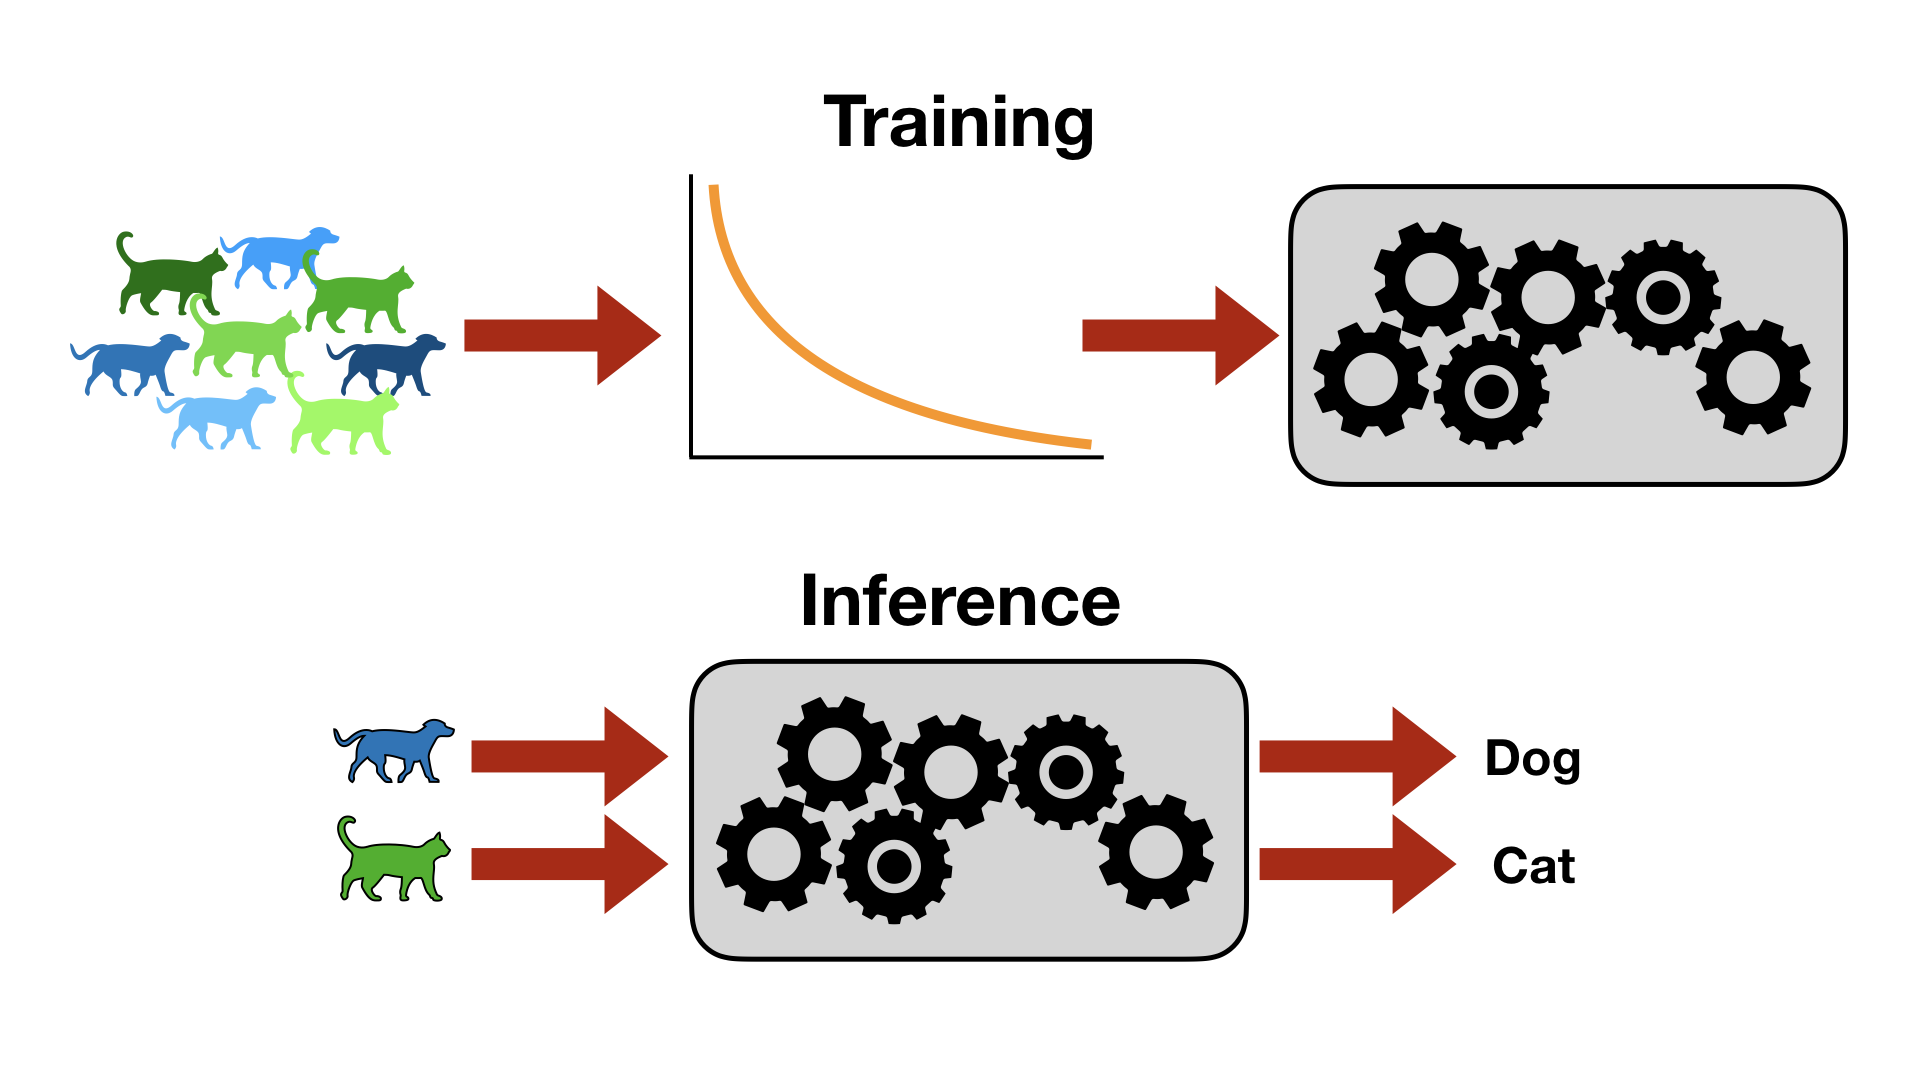
\includegraphics[trim={0 3cm 0 3cm},clip,width=0.95\textwidth]{diss/1_intro/figs/dl.png}
%     \caption[Modern machine learning pipelines]{Machine learning training and inference visualization.}
%     \label{fig:dl}
% \end{figure}
Say we have some dataset comprising of sample pairs $(x,y)$, where we wish to predict $y$ from $x$.
Our prediction, say $\hat{y}$, might be the output of some unknown function $f$ that we attempt to learn from training data. 
Let our approximation to this function be $\hat{y}:=\hat{f}(x)$.
This can take many forms, 
based on assumptions and prior information we may have on the relationships among the data. 
Consider the simple \textit{linear} case,
where we want to learn some parameter $w$ such that $y = w\cdot x$. 
Given $n$ sample pairs $(x_i,y_i)$ indexed by $i$, traditional statistics and optimization literature yield the following \textit{least squares} problem formulation, where we want to minimize the ``squared error'' between the observed values $y_i$ and the predicted $\hat{y}_i:= w\cdot x_i$:
\begin{align}\label{eq:lq}
\hat{f}:=\hat{w} = \mathop{\arg\min}_{w} \sum_{i=1}^n (y_i - w\cdot x_i)^2
\end{align}
This formulation expands without much change to a multi-dimensional form of the input $x$ and respectively, $w$: the canonical case where a number of features, or \textit{covariates} (e.g., symptoms), are used together to predict the outcome (e.g., diagnosis). 
If we are interested in which features of $x$ are important, we can look at the relative values of the learned ``weights'' $w$. In this simple setting, the importance of a feature (say $x^j$) can be exactly determined by the importance of the parameter ($w^j$).
A weight value far from zero may indicate that corresponding feature is important for diagnosis.
% If instead we are interested in which samples are most important, we can use existing methods for sample reweighting or methods that use standard assumptions to efficiently identify important subsets.

In this case and others, traditional statistical learning methods 
have been studied 
for many decades.
Linear regressors, decision trees, and support vector machines
have all been analyzed under these lenses.
% ,
% and as the modern machine learning community
% has returned to these questions recently,
% so has a renewed interest in their methods of analysis.
New research focuses
particularly on the differences
associated with moving from classical \textit{under-parametrized} models to
modern (deep) \textbf{over-parameterized} models: where
the model size vastly outnumbers the number
of input samples.
% , and may even be comparable to 
% the \textit{entire sample space.}
Methods for estimating the number of samples needed,
the time to learn a particular task,
and the generalization ability 
all require new perspectives in this regime.
While nascent, this research
attempts to fill the gap between
statistical and deep models to enable similar measures of sample influence, feature importance, and model understanding. 

\paragraph{A full picture.}
Let us expand our notation from the example above to consider this more general framing.
Consider a dataset $X:=\{x_i\}_{i=1}^n$ of size $n$ where each data point $x_i$ in the set $X$ is drawn from some underlying distribution over the domain $x_i \sim \cX^d$, 
with domain dimensionality (number of features) $d$.
A model $f$ is fit using a parametrization $\theta \in \Theta$,
with $\Theta$ the space of possible parametrizations (models) with some intrinsic dimension $p$. 
%While all three of these problems are closely related, they require different approaches. 
Generalizing the least squares``error measure'' from Eq.~\eqref{eq:lq} to an arbitrary \textit{loss} $\ell$, we have
\begin{align}\label{eq:learning}
    \hat{f}:=\hat{\theta} = \mathop{\arg\min}_{\theta\in\Theta} \sum_{x \in X} \ell(f_\theta(x_i))
\end{align}
From an analysis perspective, 
we might be interested in any one of 
(a) subsets of input features $\cC \subseteq \cX$ that are important for the downstream task,
(b) associating model subsets $\cP \subseteq \Theta$ with specific inputs or groups of inputs, or 
(c) subsets or subgroups of samples $S \subseteq \{X\}$ that are sufficient or representative of the entire dataset.

Crucially, an uninformed search for a subset is computationally infeasible. For a superset of size $n=|X|$, The set of all subsets is the power set, with a size of $2^{n}$! If an identification procedure requires looking over all of these and choosing a ``best'' one by some metric, the procedure will be limited to very small supersets.
Efficient methods have been developed in each of the three contexts above to avoid this exponential search.

\begin{figure}
    \centering
    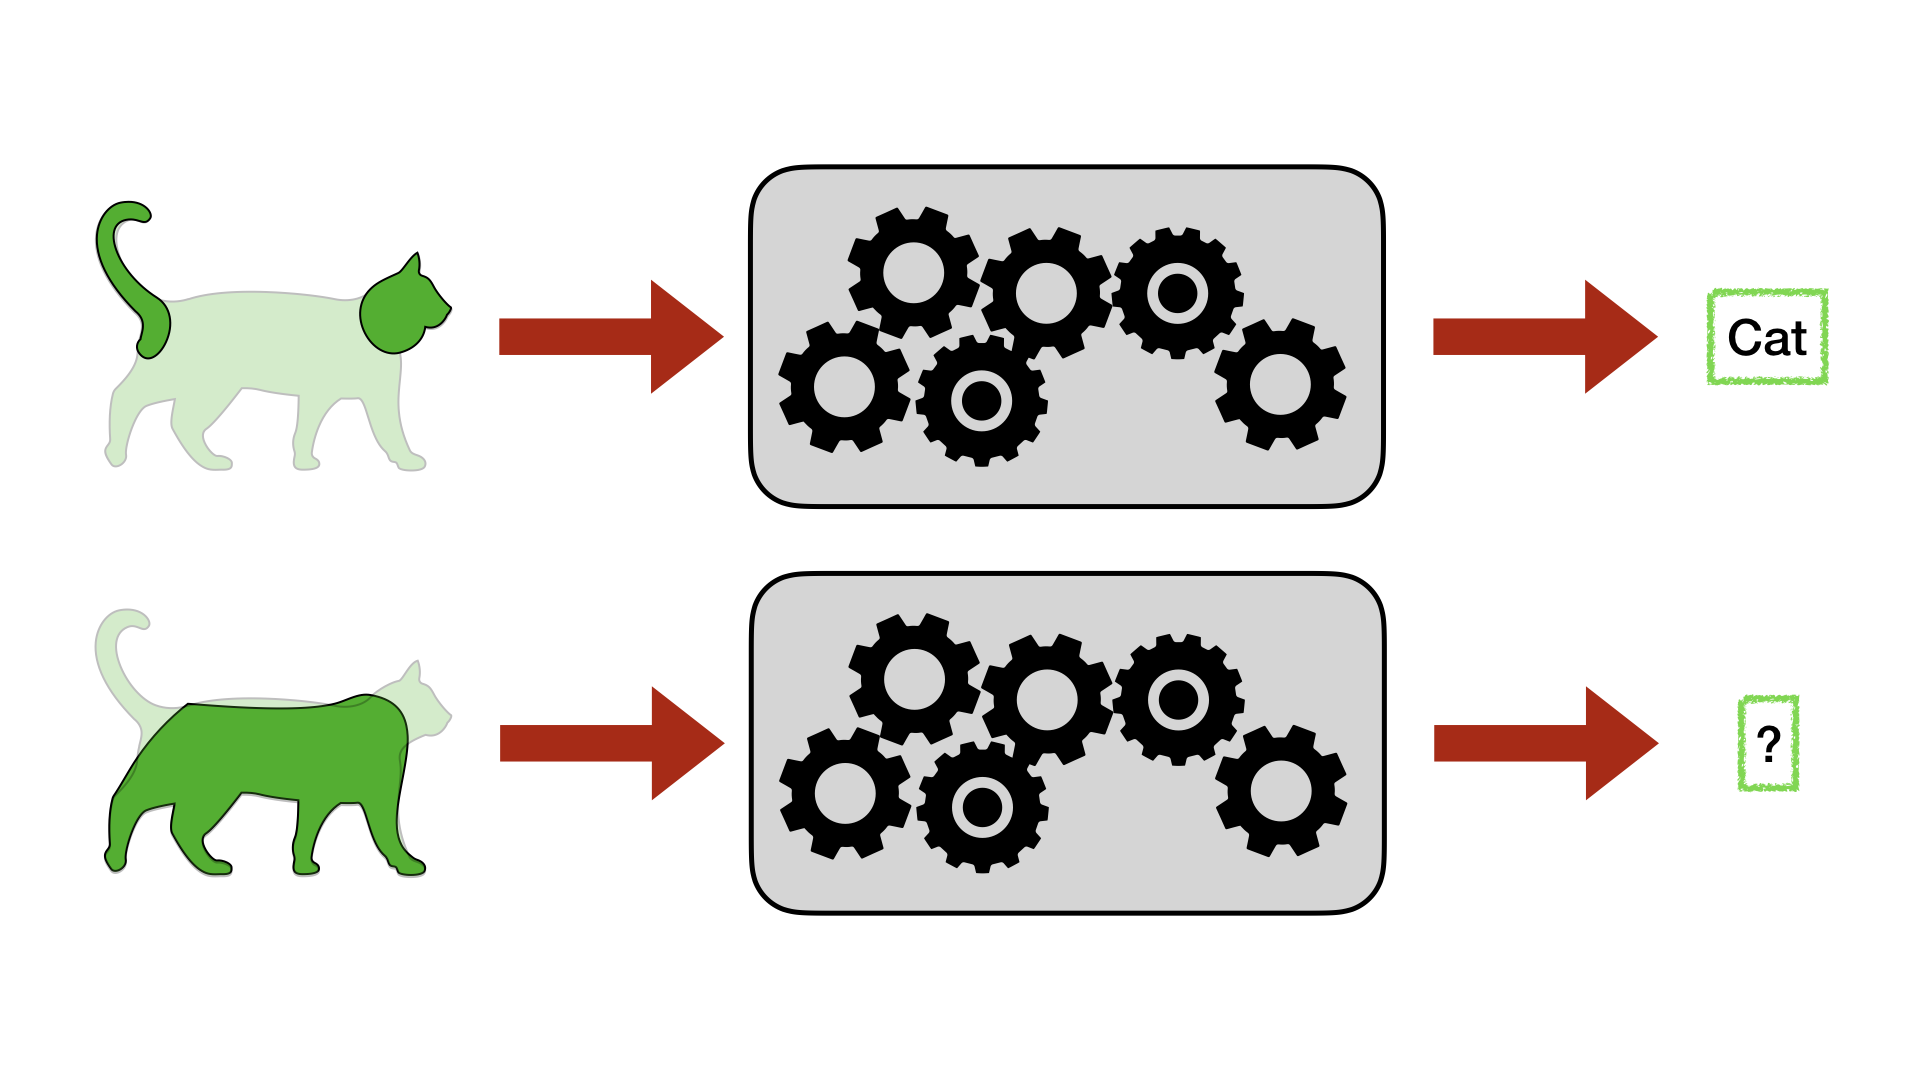
\includegraphics[trim={0 3cm 0 3cm},clip,width=0.9\textwidth]{diss/1_intro/figs/feat_select.png}
    \caption[Visualization of feature selection]{An example of identifying specific features important to the learning task.}
    \label{fig:feat_select}
\end{figure}
\paragraph{Feature Selection.} 
With more complex models $f$ compared to the linear case above, newer ``black-box'' methods have been developed for identifying important features. From the more pure statistics side, scan statistics~\citep{scanstat,scanstatlrt} allow for a structured ``scanning'' over the input space, skipping subsets unlikely to provide additional information for the measure of interest.
Further on the deep learning side, adaptations of sensitivity analysis, via noise addition and perturbations have found success~\citep{yeung2010sensitivity,zhang2015sensitivity}, alongside activation mapping~\citep{cam,selvaraju2017grad}.
These methods typically generate an analagous ``weighting'' over the input space, identifying features most salient for the specific task (Figure~\ref{fig:feat_select}).

\begin{figure}
    \centering
    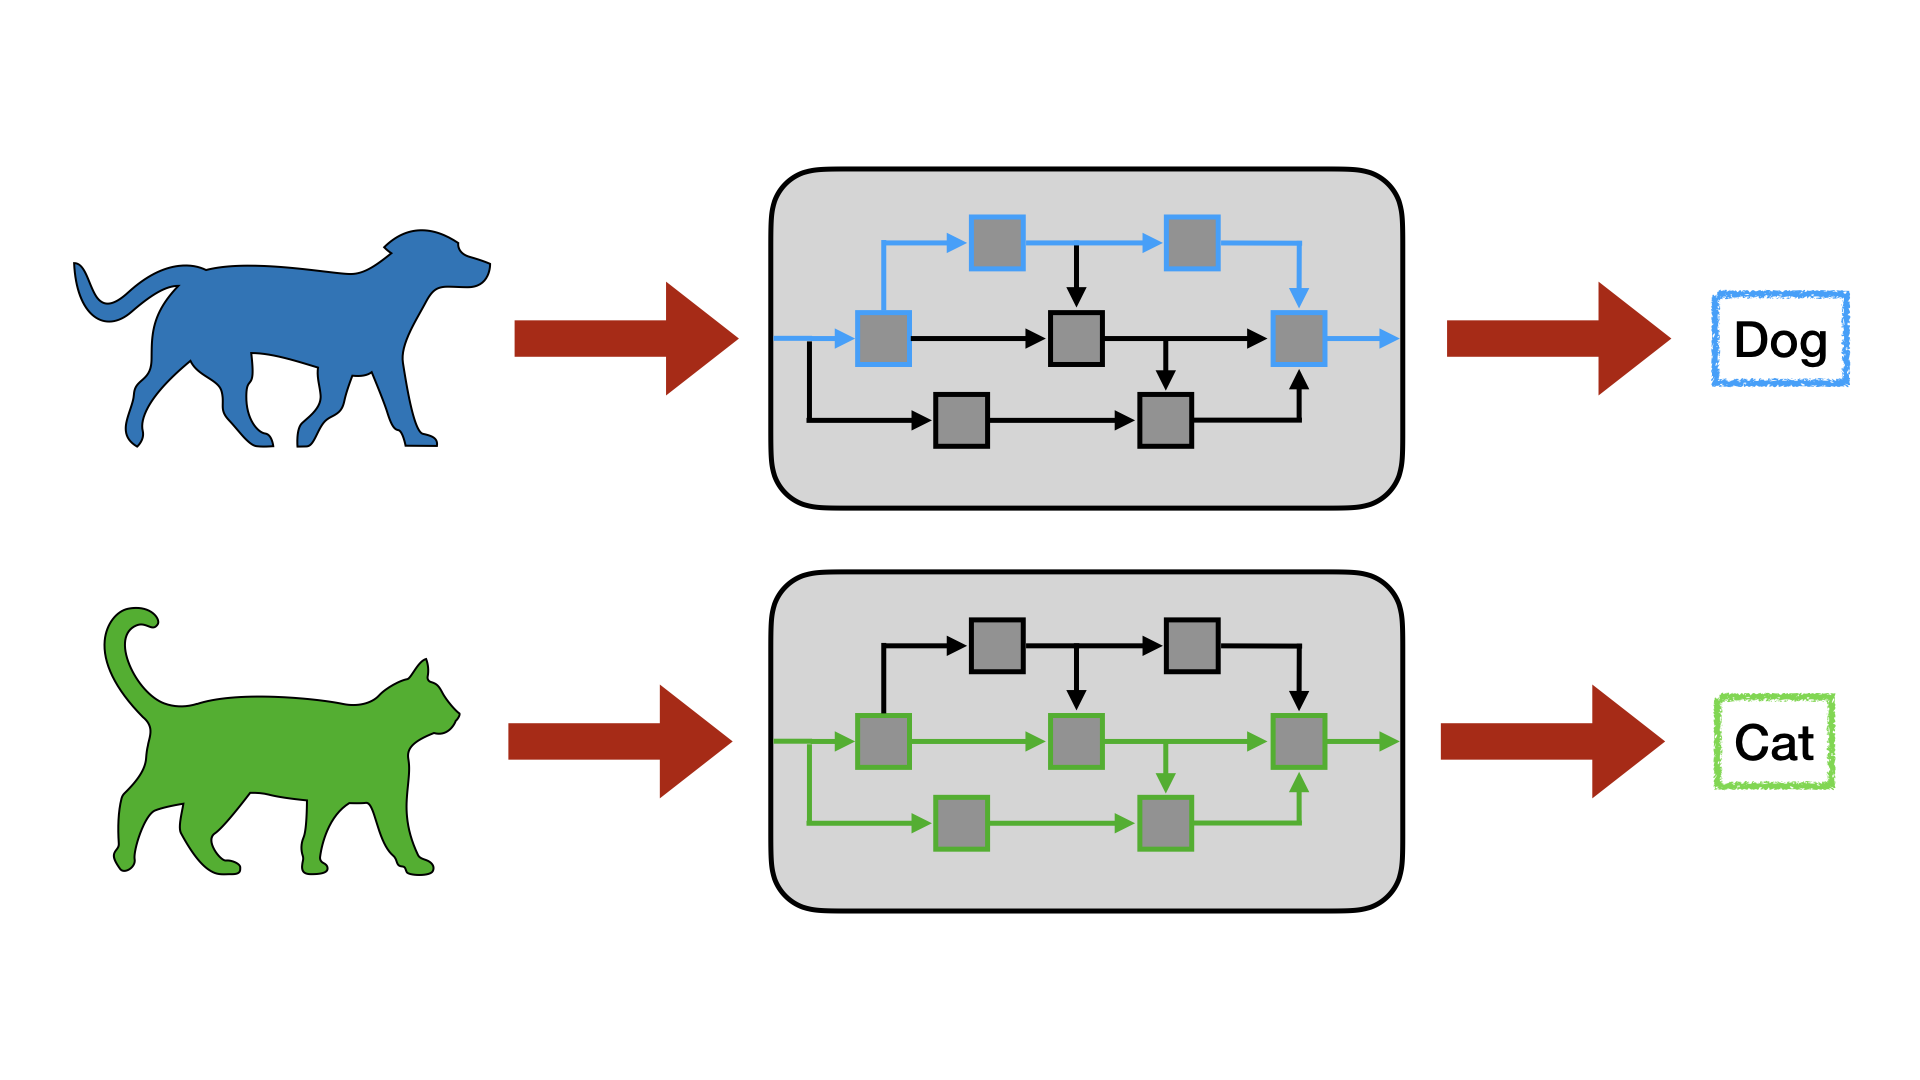
\includegraphics[trim={0 3cm 0 3cm},clip,width=0.9\textwidth]{diss/1_intro/figs/param_select.png}
    \caption[Visualization of parameter selection]{An example of identifying specific parameters important to the learning task.}
    \label{fig:param_select}
\end{figure}
\paragraph{Parameter Selection.} 
Selection in the model space generally takes two forms. First, as a prior, restriction, or assumption over the model space, and second, as a post-hoc method for an ``explainable'' proxy.
Regularization, sparsity, and gating methods are often used independent of the type or size of the model, to encourage the solution to fall within a specific region of the model space.
% In non-deep settings these methods come with strong theoretical guarantees. 
The theoretical underpinnings of these methods in deep learning are still being actively researched~\citep{hardt2016train,jacot2018neural,neyshabur2014search}, but the methods have nonetheless been effective in practice. 
On the post-hoc side, of particular interest are the parameters relevant to specific regions of the input space \textit{after} training (Figure~\ref{fig:param_select}). Here, recent analysis of deployed networks has shown this to be true~\citep{bau2017network,fong2018net2vec}, and current work continues to explore these network regions to aid in interpretability and explainability.

\paragraph{Sample Selection.} Many methods have been developed for outlier detection within training or testing sets~\citep{huang2020feature,ren2019likelihood} \textit{after} training, as well as methods for understanding sample influence~\citep{koh2017understanding,golatkar2020eternal,huang2020feature} . ``In-the-loop'' methods for accounting for ``outlierness'' behave similarly to accounting for group or individual fairness while training~\cite{mehrabi2021survey}. Unfortunately, once samples are identified in some manner, post-hoc adjustments to a trained model are generally very difficult. Recent work has focused on ``unlearning'', or removing a sample's influence on a model without retraining. If specific samples can be uniquely identified, performance and privacy reasons may require these specific interventions to reduce the ``influence'' of that sample subset.
\begin{figure}
    \centering
    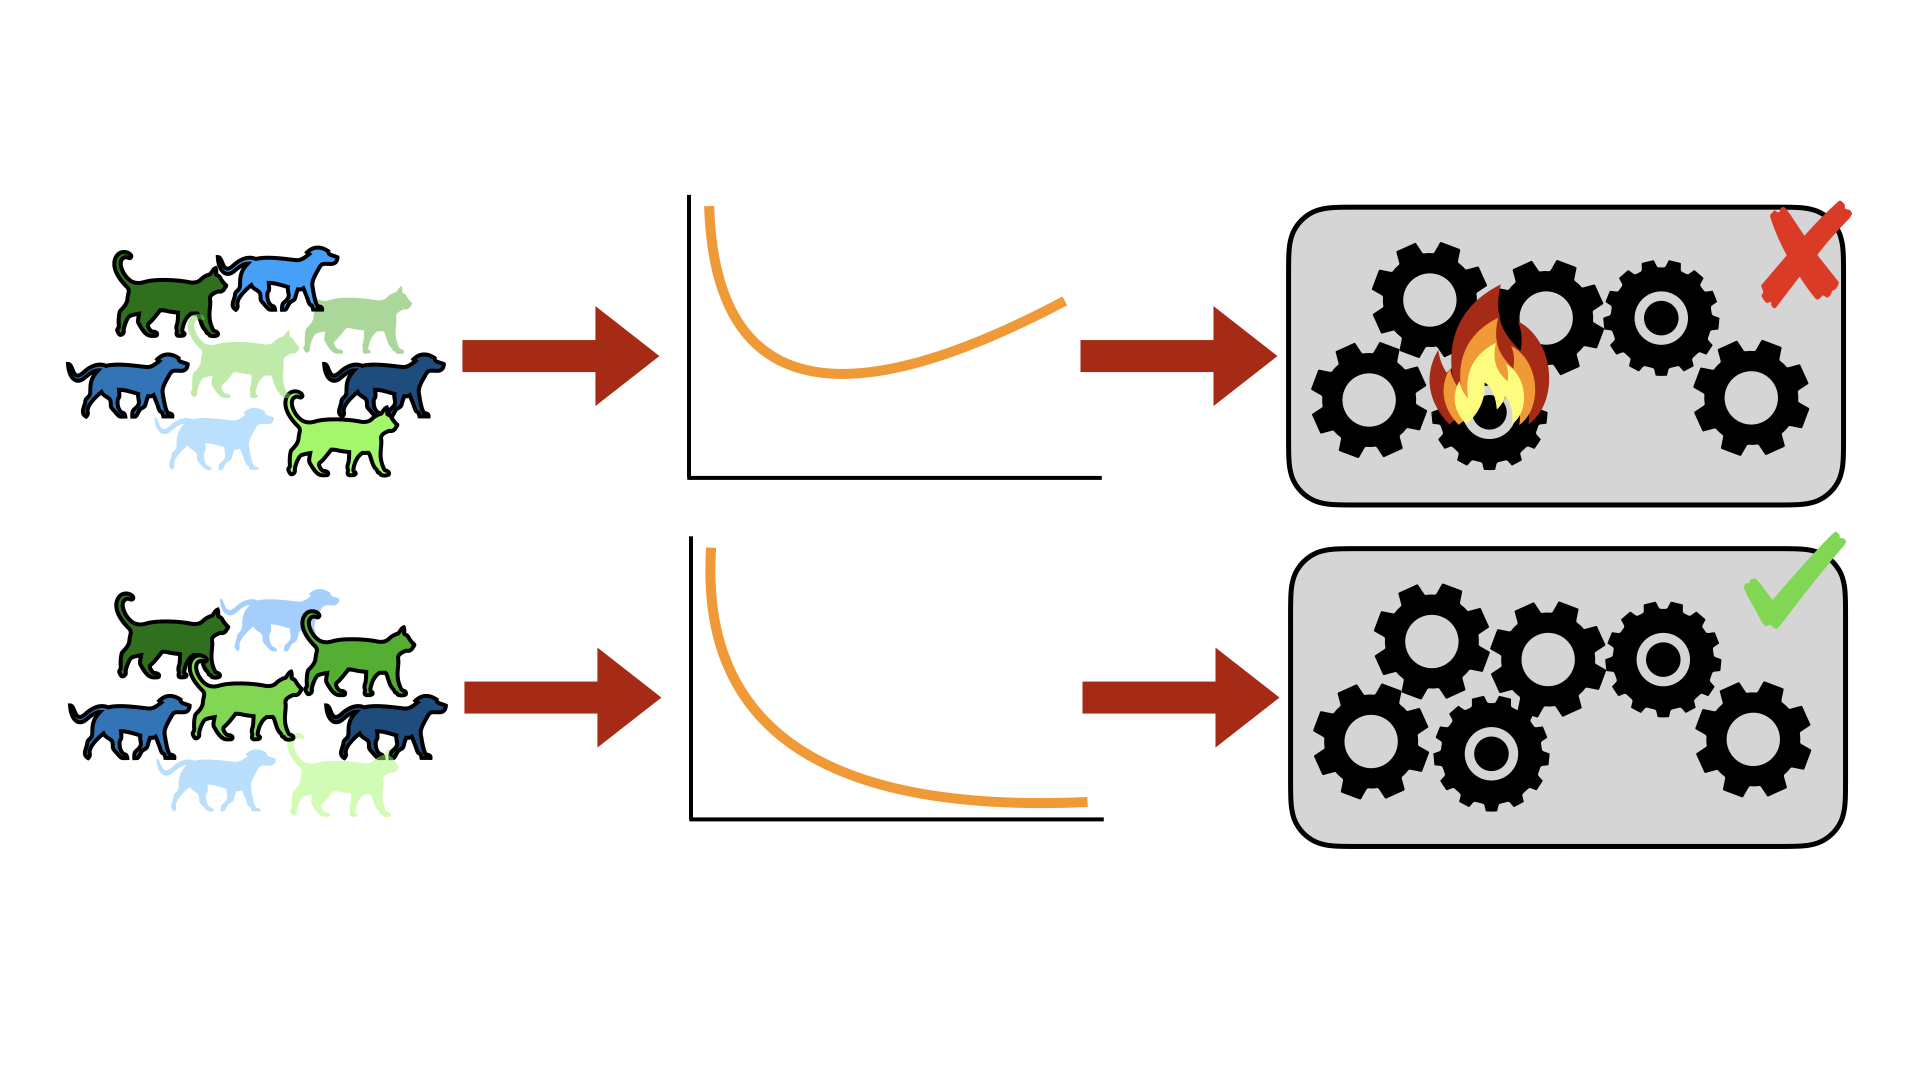
\includegraphics[trim={0 4.5cm 0 4cm},clip,width=0.9\textwidth]{diss/1_intro/figs/sample_select.png}
    \caption[Visualization of sample selection]{An example of identifying specific samples important to the learning task.}
    \label{fig:sample_select}
\end{figure}


\begin{mdframed}[style=MyFrame]
\textbf{ Thesis Goal: }
\em Identify, construct, and evaluate methods for \textbf{efficient} subset identification in modern machine learning feature, model, and input spaces.
\end{mdframed}

\section{A Few Motivating Examples}
Consider a traditional machine learning classification task in which we would like to predict whether an individual has a specific disease condition based on a medical resonance image (MRI) scan of their brain. Our input feature $x$ may consist of a 3D-array of values in $\RR^{\cI\times \cJ\times \cK}$ measuring some intensity of the imaging modality at each voxel, indexed by a tuple $(i,j,k) \in (\cI,\cJ,\cK)$.
Our outcome variable $y$ may simply be a binary label of whether the input scan has been labeled by a radiologist as one demonstrating typical disease characteristics.
Using an off the shelf 3D convolutional neural network with adjustments to match our input size, we can very quickly set up and train a system to predict disease presence with a high degree of accuracy.

\paragraph{Example 1.}
With a prediction for a specific scan, or predictions over a number of scans, we might be interested in identifying which regions of the brain are most important for diagnosis. These regions, $R \subset \cR:=\RR^{x\times y\times z}$, can be specific groups of pixels in the image that may correspond to known functional networks. Methods such as attention and class activation maps may work here, but there are a few issues. The number of samples available to learn a model is very small compared to the both the dimension of the input and the number of parameters in the model, i.e., $n \ll p$ and $n \ll d$. Thus it is very easy to overfit, and for areas of interest to be associated with intricacies of particular input data rather than true, real differences defined by the disease.

Furthermore, recent medical imaging studies have moved past simple difference detection: trends over time, and the ability to predict {\em future} disease development have by far become the setting of most interest.
Given an image of a healthy individual, is it possible to predict what their scan, or their future disease diagnosis, may be up to 10, 20, or more years in the future?
If a number of scans have been collected over some timeframe, can the \textit{trajectory} of the individuals' development be extrapolated to estimate progression?
As traditional models extended for temporal analysis grow in both size and complexity,
a number of subproblems explicitly related to model and input subspaces arise. In this thesis we address two such problems: \textbf{statistically rigorous identification of temporally evolving subsets}, and \textbf{characterizations of deep models that enable efficient training of recurrent models with large scale time-varying data}.
    
\paragraph{Example 2.}
With the rapid growth of AI and machine learning applications has come valid concerns regarding both guarantees of privacy.
Recent technology legislation has made the importance clear in all aspects of data use,
and particular projects and groups have demonstrated that machine learning is not independent of
this need \citep{Exposing}.
A new issue raised within this intersection is the ``right to be forgotten".
If a model has been trained with a particular users' data, 
they should have some recourse or right
to both remove their data from the training set,
and also know that the model has not learned from their data.
On the surface, this poses a significant problem for model builders
and organizations that spend large amounts
of time and resources in 
training deep learning models.

In the medical imaging example above this is especially important: with fewer samples it is more likely that information about any particular one could ``leak'', and the model's performance may degrade significantly as a relatively large percentage of it's training data is removed.
Thus tailored methods must be developed to ensure both privacy and performance, without requiring full retraining.
As we will see, 
\textbf{identification of model parameter subsets}
that are particularly important
for a particular sample's influence
in a model enables \textit{efficient machine unlearning}.

\paragraph{Example 3.}
From an alternative perspective, we may want to identify specific samples rather than have them specified a priori.
Traditionally a rigorous area of study under classical statistics, outlier detection and accounting have become a subfocus for many within the machine learning community as well \citep{golatkar2020eternal,golatkar2020forgetting,huang2020feature,ren2019likelihood}.
While subgroups of input samples may be outliers, it is more often the case that they represent known heterogeneity within the data. 
These differences may be marked using 
group information known a priori, and 
most learning tasks aim to learn tasks
in a \textit{subgroup-independent} manner.
In our disease prediction model above,
these groups could simply be stratified by the type of scanner used to acquire the image, but it could also
be a systematic difference correlated with some protected attribute. {\color{red} sentence about original brain atlas for registration being eurocentric}
This can directly lead to disparate performance and results on \textit{all} individuals outside of that group.
Optimization and regularization methods with this focus come under the umbrella of model fairness.
However, many existing methods do not scale well to larger models or as the number of subgroups grows, as is often the case when intersections of protected classes must be considered. Here we identify and construct a particular solution for \textbf{groupwise fairness that enables efficient in the loop fairness regularization}.

% What features are most important for prediction?
% Which samples were most important for my training?
% Can we understand when a model is certain or uncertain about its output?
% Are there layers in my network that have learned a particular subtask?
% Questions of robustness, bias, influence, fairness, and importance have become central questions to contemporary machine learning research \citep{doshi2017towards,mehrabi2021survey,amodei2016concrete}.
% machine learning, etc.

% Feature selection in the case of
% typical regression or classification 
% takes some form of learning parameters $\theta$ that allow for $\hat{y} = f_\theta(x)$ to be close to the true outcome of interest $y$.
% While forms of data $X := (x,y)$ may simply be continuous and real-valued, modern machine learning has greatly expanded formulations of the classical learning problem to include a wide variety of structured learning problems~\citep{nowozin2011structured}. 
% Consider the case when a high-dimensional input is used to predict an output with a highly-parametrized model. 
% Once learned, obvious questions arise as discussed above: are there specific low-dimensional spaces in either the input or the model space that are most important or necessary for the global learning problem of interest? Are there specific subspaces associated with particular subproblems of the global problem?
% The machine learning literature has come up with a number of ways to identify analogs of these spaces, 
% including extensions of sensitivity analysis to deep learning~\citep{yeung2010sensitivity,zhang2015sensitivity}, and constructing and identifying nonzero model subsets via particular model choices such as activations~\citep{selvaraju2017grad} and regularizers.
% In classical settings these are well understood: decision trees naturally provide ease of interpretibility via the information used to choose splits, and both linear and kernel support vector machines have been analyzed to provide for measures of sample importance via distances to the margin as well as feature importance via weights defining the learned hyperplane~\citep{Mitchell97}.
% Attention and saliency maps have emerged as popular new methods,
% given their ease of implementation and interpretation~\citep{sutskever2014sequence,vaswani2017attention,selvaraju2017grad}.
% By learning dimensions of a given input that are particularly important, either in a hard (binary) or soft (continuous weighting) manner, model builders are better able to understand and interpret what a model has learnt.
% The specific ideas of attention notwithstanding, many of these existing methods are far removed from traditional hypothesis testing frameworks.
% While some work has begun in this direction~\citep{tansey2018black},
% there remains a gap in direct identification of subsets and structures in these spaces that can be defined in statistically rigorous manners.

% \begin{figure}
%     \centering
%     \includegraphics[width=0.5\textwidth]{example-image-a}
%     \caption[A simple subset selection example]{\color{red} Identifying and selecting in MRIs, subset, sample, model ID.}
% \end{figure}

% \paragraph{A specific example.} 

% ------------------------------------------

% below here will be moved and arranged with the "selection" sections and here if relevant

% ------------------------------------------

% While attention can be directly applied to the network in order to identify ``hotspots" in the input space relating to the learned classification task, 
% given the high-dimensional nature of the input
% and the relatively small sample size 
% associated with medical imaging data, 
% it is very likely that an area of interest identified
% may be an intricacy of the training samples used rather than truly a region of disease signal.
% Class activation maps (CAMs) may be unclear, and can often associate with image artifacts unrelated to the scientific task~\citep{adebayo2018sanity}.
% Methods of generalization may help to increase confidence in identified regions, but statistical guarantees often remain out of reach.

% Furthermore, most recent problems associated with medical data have moved past simple difference detection: trends over time, and the ability to predict {\em future} disease development has by far become the setting of most interest.
% Given an image of a healthy individual, is it possible to predict what their scan, or their future disease diagnosis, may be up to 10, 20, or more years in the future?
% If a number of scans have been collected over some timeframe, can the \textit{trajectory} of the individuals' development be extrapolated to estimate progression?
% As traditional models extended for temporal analysis grow in both size and complexity,
% a number of subproblems explicitly related to model and input subspaces arise. Here we address two such problems: \textbf{statistically rigorous identification of temporally evolving subsets}, and \textbf{characterizations of deep models that enable efficient training of recurrent models with large scale time-varying data}.

% A sample's particular influence on model parameters aside, the identification of influential samples or subsets of samples more generally is of independent interest. 
% Traditionally a rigorous area of study under classical statistics, outlier detection and accounting have become a subfocus for many within the machine learning community as well \citep{golatkar2020eternal,golatkar2020forgetting,huang2020feature,ren2019likelihood}.
% While subgroups of input samples may be outliers, it is more often the case that they represent known heterogeneity within the data. 
% These differences are typically marked using 
% group information known a priori, and 
% most learning tasks aim to learn tasks
% in a \textit{subgroup-independent} manner.
% Optimization and regularization methods with this focus come under the umbrella of model fairness, and instead of identifying and boosting independences within the model or data, we aim to minimize them.
% However, many existing methods do not scale well as the number of subgroups grows, as is often the case when intersections of protected classes must be considered. In the sequel we identify and construct a particular solution for \textbf{groupwise fairness that enables efficient in the loop fairness regularization}.

\begin{mdframed}[style=MyFrame]
\em 
Here we focus our effort on identifying these important subsets of model, feature, and sample space for feature association, model size reduction, model unlearning, and, fairness. Specifically, taking advantage of both existing statistical and geometric methods, we develop new methods for localizing subsets in a range of settings from hypothesis testing to deep learning.
\end{mdframed}

\section{Thesis Scope and Contributions}

We explore the intersections of classical statistical and geometric constructions with modern machine learning methods. 
Figure~\ref{fig:scope} shows the overall scope projected along three axes: feature, parameter, and sample spaces.
Below we briefly introduce the main problems studied in this thesis.
\begin{figure}[!ht]
    \centering
    % \includegraphics[width=0.99\linewidth]{scope.pdf}
    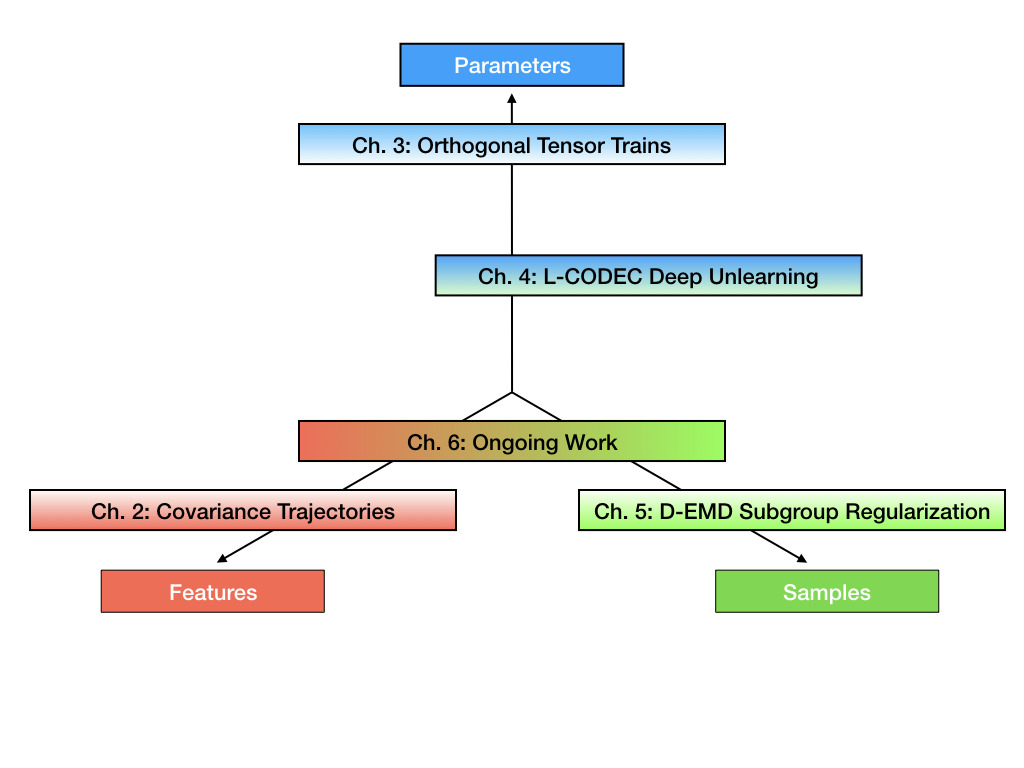
\includegraphics[width=0.95\linewidth]{diss/1_intro/figs/thesis_scope.png}
    \caption[Thesis Scope]{Thesis scope, projected over three representative axes. {\color{red} update chapter numbers shift by 1}}
    \label{fig:scope}
\end{figure}

\subsection{Second-Order Modeling and Group Difference Analysis over Time}

Recent results in coupled or temporal graphical models offer schemes for estimating the relationship structure 
between features when the data come from
related (but distinct) longitudinal sources. A novel application of these ideas is for analyzing group-level differences, i.e., in identifying if {\em trends} of estimated objects (e.g., 
covariance or precision matrices) are different across disparate conditions (e.g., gender or disease). Often, poor effect sizes make detecting the \textit{differential} signal 
over the {\em full} set of features difficult: for example, 
dependencies between only a {\em subset of features} may manifest differently across groups.
We first suggest
a parametric model 
for estimating trends in the space of $\SPD$ matrices as a function of one or more covariates.
We will then generalize scan statistics to graph structures, 
to search over distinct subsets of features (graph partitions) whose temporal dependency structure may show statistically 
significant group-wise differences.
We will theoretically analyze the Family Wise Error Rate (FWER) and bounds on Type 1 and Type 2 error. 
On a cohort of individuals with risk factors for Alzheimer's disease (but otherwise cognitively healthy), 
we 
find scientifically interesting 
group differences where the default analysis, 
i.e., models estimated on the full set of features, do not survive reasonable 
significance thresholds. 
% Preliminary work on this was published in \citep{covtraj}.


\subsection{Efficient Tensor Representations for Feasible Temporal Deep Learning}

Modern deep networks have proven to be very effective for analyzing real world images.
However, their application in medical imaging is still in its early stages,
primarily due to the large dimension of three-dimensional images, requiring enormous convolutional or fully connected layers --
if we treat an image (and not image patches) as a sample. 
These issues only compound when the focus moves towards longitudinal analysis
through recurrent structures, and when a point estimate of model parameters is insufficient 
in scientific applications where a reliability measure is necessary.
Using insights from differential geometry, 
we will adapt 
the tensor train decomposition to construct networks
with significantly fewer parameters,
allowing us to train powerful recurrent networks on whole brain image volumes. 
We analyze 
the \textit{orthogonal tensor train},
and demonstrate its ability to express a standard network layer both theoretically and empirically.
We 
demonstrate its ability to 
effectively reconstruct whole brain volumes
with faster convergence and stronger confidence intervals
compared to the standard tensor train decomposition. 
We provide code and show experiments on the ADNI dataset
using image sequences to regress on a cognition related outcome.
% Preliminary work on this was published in \citep{ott}.

\subsection{Practical Unlearning via Large-Scale Conditional Independence Testing}

%With AI systems extensively using personal %data for model training, 
Recent legislation has
led to interest in {\em machine unlearning}, i.e., removing specific training samples from a {\em predictive} model as if they never existed in the training dataset. 
Unlearning may also be required due to  corrupted/adversarial data or simply a user's updated privacy requirement.
For models which require no training ($k$-NN), 
simply deleting the closest original sample can be effective. 
%However, it is not clear how such approaches can be used to unlearn 
%models that contain rich information learned from the original data.
But this idea is inapplicable to models which learn richer 
representations.
%from data. 
%Recently, optimization-based unlearning estimators have been proposed, but 5their 
Recent ideas leveraging optimization-based updates
scale poorly with the model dimension $d$,  
due to 
inverting the Hessian of the loss function. %with an overall cost of $O(d^3)$ 
%is prohibitive.
We describe
a variant of a new conditional independence coefficient, 
L-CODEC, to identify a subset of the model parameters with the most semantic overlap on an individual sample level. 
Our approach completely avoids the need to invert a (possibly) huge matrix. 
By utilizing a Markov blanket selection, 
we find
that L-CODEC is also suitable for deep unlearning,
as well as other applications in vision.
Compared to alternatives, L-CODEC makes approximate unlearning possible 
in settings that would otherwise be infeasible, 
including vision models used for face recognition, 
person re-identification 
and NLP models that may require unlearning samples identified for exclusion.
% Preliminary work on this will appear in \citep{lcodec}.


\subsection{Reducing Subgroup Fairness via High Dimensional Earth Mover's Distances}

Optimal transport has recently emerged as a useful tool for machine learning through its connections with geometry, statistical machine learning, and through practical algorithms. Existing methods that leverage optimal transport often  regularize using  a Wasserstein metric or by computing barycenters, for example. %which are effective when distributions are continuous and known, or when measures of interest are discrete.
% Our formulation allows for a discretization of continuous measures that drop in directly to classical  formulations of the Earth Mover's Distance. 
We leverage optimal transport, except that we take advantage of a recently-introduced algorithm that computes a generalized earth mover's distance.
Not only is this algorithm computationally cheaper to compute compared to existing barycentric measures, but our method has the additional  advantage that gradients used for backpropagation can be directly read off of the forward pass computation, which leads to substantially faster model training.
We provide technical details about this new regularization term and its properties, 
and 
experimental demonstrations of improved training speed over existing Wasserstein-style methods.

{\color{red}
\subsection{Understanding Latent Spaces via Conditional Independences}

The final chapter of this thesis applies some of the tools developed above in the analysis of latent spaces in recent large scale models.
% In these studies, 
% we aim to identify conditionally independent features and subjects that are particularly important to the prediction and estimation of
% key disease outcomes,
% as a function of a number 
% of demographic, neuropsychological,
% genetic,
% and imaging data collected as 
% part of an ongoing consortium 
% to understand the progression
% of Alzheimer's disease in younger, 
% asymptomatic populations.
% In what follows we present
% exploratory analysis
% on a small, easily 
% digestible subset of the available data,
% that lays the foundation for
% further analysis.
}
% This work is the most forward looking, and aims to be a stepping stone toward a rigorous 

\section{Outline}
Chapter 2 covers the essential background necessary for the developments presented in the following chapters, including specifics of graphs and hypothesis testing, as well as relevant modern methods for learning and optimization.
In Chapters 3 through 7, we describe four perspectives to address subset identification.
Chapter 3 explores and focuses on the identification of feature subsets varying over time.
In Chapter 4 we describe a method of constraining the parameter space in a particular manner
that enables more efficient large scale neural networks.
Next, Chapter 5 provides a solution to the machine unlearning problem,
enabled through a particular conditional independence parameter selection scheme, vastly reducing network update costs.
Chapter 6 ends with a unique solution to subgroup fairness, 
where we take advantage of an efficient solution to
the $d$-dimensional earth mover's problem
to regularize large models when the number of subgroups can be large.
{\color{red} Chapter 7 describes future work, focused on applying a particular solution from Chapter 5 to understanding relationships among features in latent spaces learned by large generative models.}


%%%%%%%%%%%%% 
% Some old stuff

% Significant progress in the modern development of machine learning has
% been built upon connections and patterns identified across myriad
% interdisciplinary fields of study.
% Up through the mid 2000's, 
% many of these methods were inspired by and interested in 
% highly focused and constrained problems. 
% With a reasonably sized input domain, could a model of roughly equal size be used to
% predict some output?
% Linear regressors, decision trees, and support vector machines were all answers to these questions, with their own
% varying degrees of scaling and complexity.
% These methods necessitated carefully constructed formulations with specific restrictions to the learnable function class,
% enabling straightforward analysis 
% for provable performance guarantees 
% and easy identification of critical training samples and important input features.

% Contemporary machine learning, however, has a vastly different modus operandi. 
% Driven in large part by the exponential growth of available computation via Moore's Law, \textit{deep learning} has fallen squarely in the realm of \textbf{over-parameterized} models.
% With these overparametrizations and computation capacity, the typical learning questions posed as maximizing accuracy or reducing error have largely been addressed for even large scale problems.
% As such, complementary questions have led to subfields focusing on other performance measures, such as robustness, fairness, interpretability, and explainability.
% Many solutions to these questions end up looking back at answers found for the under- or non-parametrized settings.
% While nascent, these approaches 
% attempt to fill the gap between
% statistical and deep models to enable similar measures of sample influence, feature importance, and model analysis. 
% Most notable amongst these newer approaches is that of (Self)-Attention in Neural Networks \citep{sutskever2014sequence,vaswani2017attention}.
% Other proposals 
% end up looking back at the types of analysis typical of those more classical under-parametrized or nonparametrized methods.

% Not limited to previous developments in learning or computation theory, the arguably most valuable contributions toward the exponential reduction in model error can be attributed to influences and intuitions taken
% from biology, psychology, neuroscience, and even XXX \citep{srivastava, etc}.
% Perhaps one explanation as to why this phenomenon exists may be attributed to the way in which deep learning evolved. 
% The classical learning goal of function approximation lends itself nicely to a system which allows for arbitrary complexity via simple changes (e.g., addition of neural network layers). % Foundational works building on the original neural networks particularly have taken advantage of constraining this space of functions to search over: 
% the most seminal case being those of convolutional filters for imaging data. 
% While ``constraints" of this form have helped tremendously in model performance on modern vision and language machine learning tasks (GANs, Recurrent Networks, Residual Layers, Transformers, etc.), the ability to identify \textit{subsets} of important samples, input features, and model parameters has lagged significantly behind the development of these methods.
% Recently larger interest has been taken by the community to understand and interpret models with this view, only after extremely large and opaque models have become ubiquitous.
%This lag directly explains the more recent interest in developing methods for understanding and interpreting large scale machine learning models.
\chapter{Introduction} \label{chap:intro} 

Modern applications of machine learning in a broad range of industrial and consumer-facing systems have become ubiquitous.
Most interactions with daily technologies now intrinsically involve 
a request to some ``smart`` system in the ``cloud'', 
where those interactions range from
a request for map directions 
to simply loading a webpage.
Neural network models, and the recent advances of deep learning,
have enabled these systems that 
make such applications possible.
These models have achieved
human-level performance on learning tasks
including image classification~\citep{resnet,alexnet}, image segmentation~\citep{segmentation}, video analysis~\citep{zhang2016video}, text understanding and generation~\citep{bert,gpt}, and have slowly begun to solve more fundamental scientific problems such as protein folding~\citep{protein} drug discovery~\citep{drugdisc}, and medical diagnosis~\citep{diag}.
While this performance is largely attributed to model size,
the abundance of high quality training data
has equally contributed to real world performance,
enabling model training over millions of real world samples~\citep{imagenet,laion},
and potentially billions of synthetic samples via environment simulation~\citep{mcts}.

While deployment in some domains (recommender systems, object detection) may benefit almost unconditionally from this vastly expanded capability, rightful hesitancy has limited their widespread use in particular applications where impacts on individuals, people, or environments may be at stake.
These ``last mile'' concerns take a few forms.
% Because a completely accurate model is still out of reach, an important question that needs to be answered is: which inputs or individuals are being given incorrect outcomes, and why?
% maybe a sentence suggesting unlearning/removal
In mission critical applications such as medical diagnosis, 
the impact of an error can be extremely large,
even if a misprediction happens extremely infrequently.
Additionally, large scale model training and architecture search
can require exorbitant amounts of energy producing high emissions,
and their scale can limit market participants
to only large actors with vast existing resources.
The accessibility and effectiveness of these models can also vary significantly based on the training data, and disparate outcomes can be exacerbated by existing social inequity.

While existing human or ``natural'' systems that these models aim to assist are not perfect, 
our real world has developed norms and regulations that 
enable them to function.
A medical diagnosis might require a physician to explain what symptoms led them to that particular conclusion.
Energy metering and carbon taxes may be applied to limit
emissions.
Regulatory satisfaction may require 
analysis proving equal opportunity,
or that specific protected classes
are not used in decision making.
% Specifically, these can include ideas as simple as the Hippocratic Oath and medical malpractice insurance, to asking your doctor what symptoms lead them to a particular diagnosis.
These ideas are difficult to directly translate to automated machine learning systems,
but proxies have been identified that we can build upon.

These norms and regulations answer a number of questions we may also try to pose to our machine learning models.
What is the cost to learn this task?
What led to this particular outcome?
Why is this outcome different from another?
% We will explore how these questions can be formulated concretely. 

If the answer to these questions is negative or unknown,  follow-up questions all take an interesting form:
Can we learn a smaller model with similar performance? 
Can we identify the most important features? 
Which individuals or groups are being treated unfairly, and can we change that?
These questions ask us to identify a \textit{subset} of some relevant set, dependent on setting, and this identification is our focus here.

% Moving specifically to machine learning methods,
Taking a step back, let's take a look at a representative system. Figure~\ref{fig:dl} illustrates a typical learning pipeline. 
A dataset is collected and used to train a model, by minimizing the error over
those samples in the dataset (top).
A ``sample'' can be a single measured value, or it can
be a large, highly structured object with many ``features.''
The model is made up of some ``parameters'' that are 
tuned during training to learn a good predictor over the training dataset.
This model is then used to predict, or \textit{infer}, on new
data seen ``in the wild'' (bottom).
Our questions above are formally asking to identify \textit{subsets of these objects}: is a subset of the model parameters sufficient for learning? Which subset of the features are important for a prediction? Which subset of the dataset exhibit a specific attribute?
\begin{figure}
    \centering
    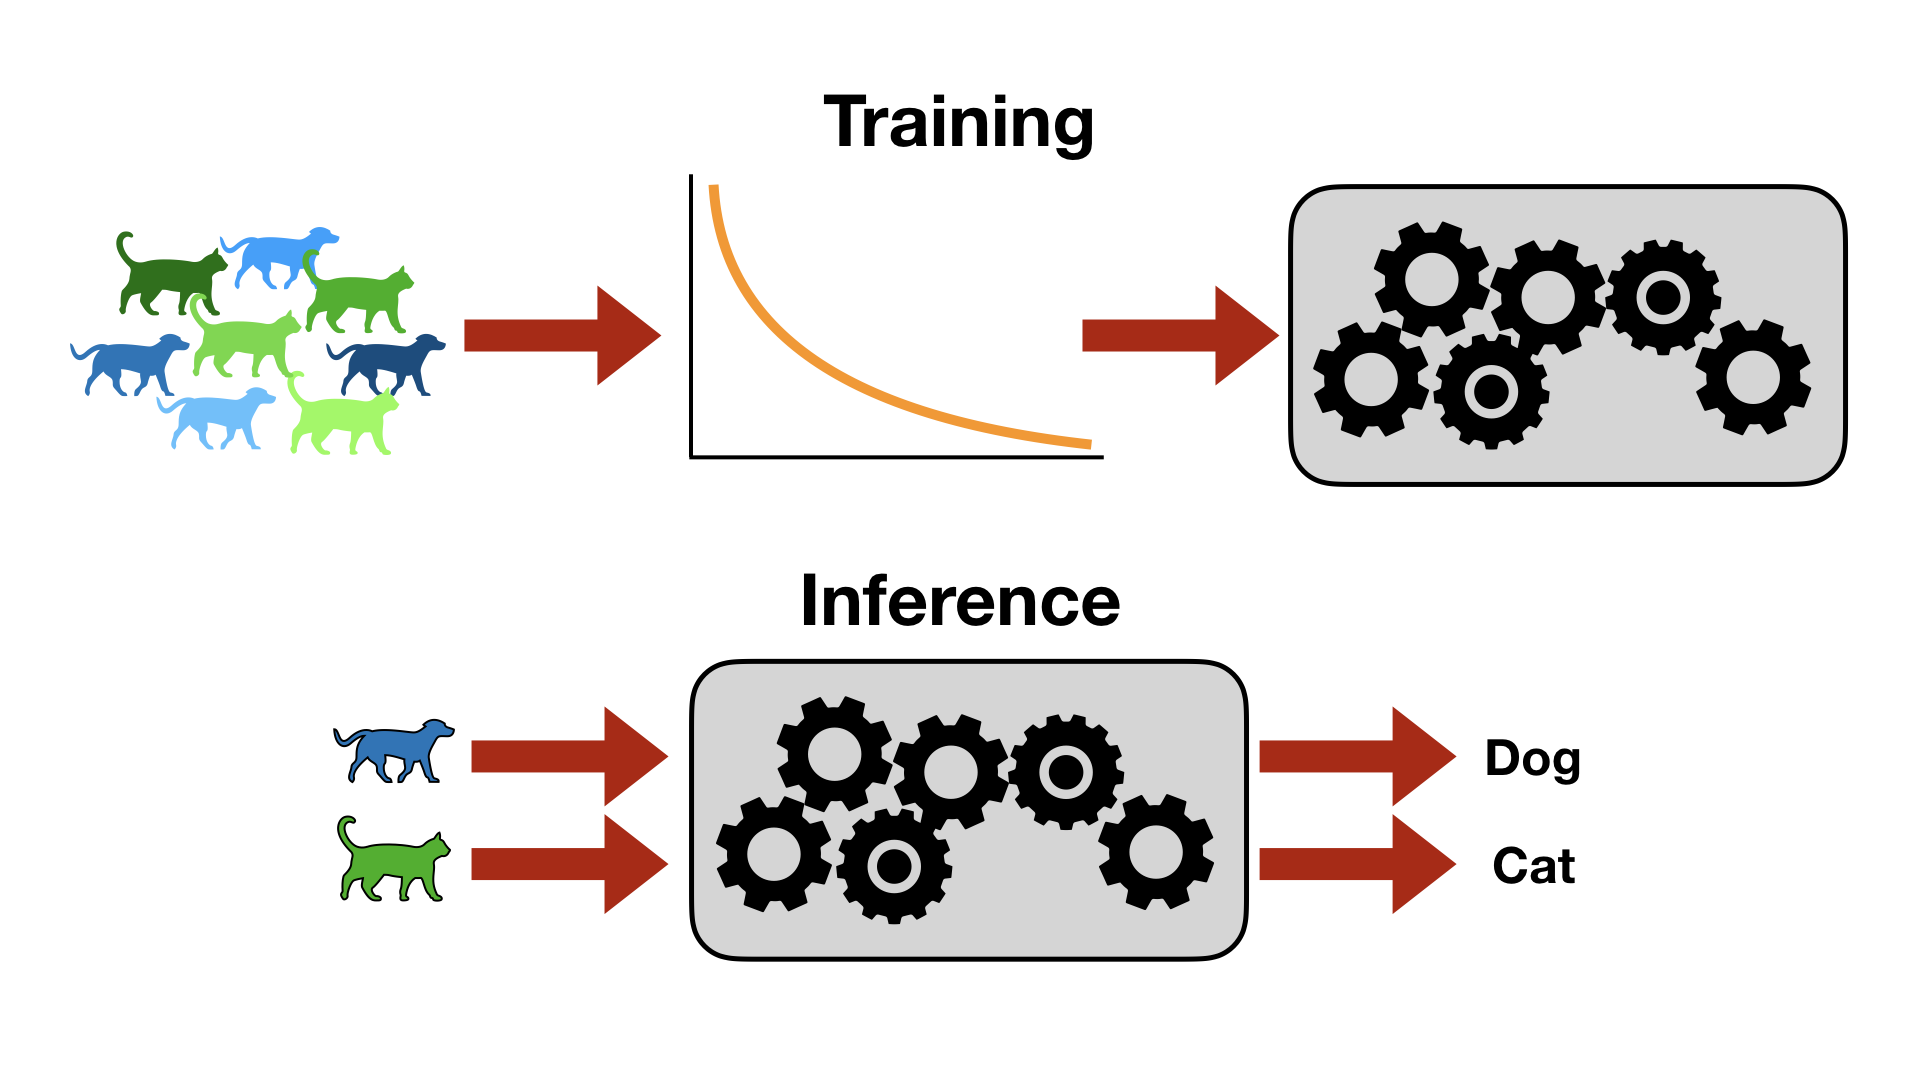
\includegraphics[trim={0 3cm 0 3cm},clip,width=0.95\textwidth]{diss/1_intro/figs/dl.png}
    \caption[Modern machine learning pipelines]{Machine learning training and inference visualization.}
    \label{fig:dl}
\end{figure}

% \textit{Explainability} can be seen as identifying important features of the input, as well as parts of the model (parameters) that ``light up`` for that input. \textit{Fairness} can be evaluated via measures over subsets of the data that correspond to specific groups. 

\begin{mdframed}[style=MyFrame]
\em 
\textbf{This thesis} focuses its main efforts on identifying these important subsets of model, feature, and sample space, to enable answering questions necessary for mainstream adoption of machine learning methods.
\end{mdframed}

% In this dissertation, we explore the sizes of these models, samples, and datasets, and 
% analyze under what situations 
% a smaller \textit{subset} of them may be sufficient or important
% for questions that run parallel to standard performance and accuracy measures.

Let us step a bit deeper into a basic illustrative example. In order to ease understanding, we can first begin with a basic formulation of learning methods, from which the questions above can take specific forms. 
Learning methods typically  try to identify a function mapping (model) that is able to complete a specific task at some high level of profficiency.
% In Figure~\ref{fig:dl}, a model is trained using examples of classification task (top), in order to accurately predict the class of a newly provided input (bottom).
% \begin{figure}
%     \centering
%     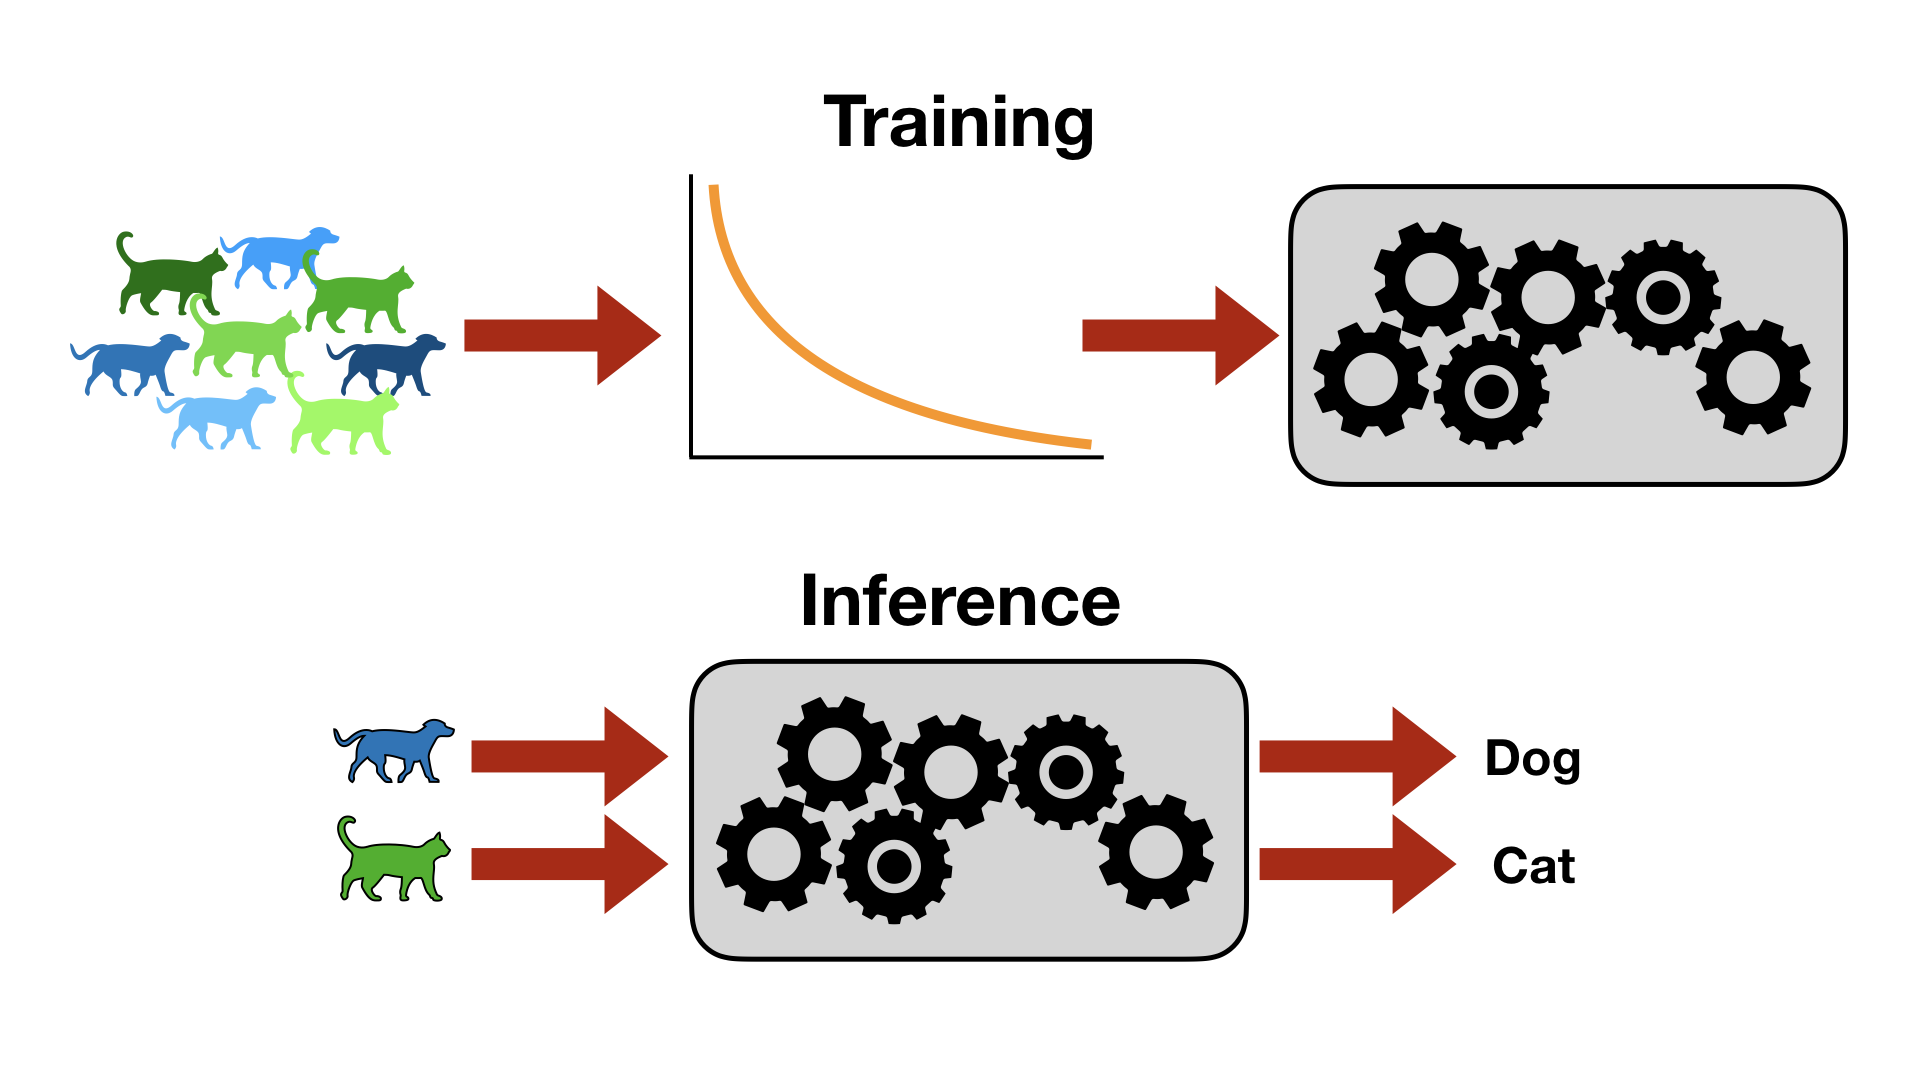
\includegraphics[trim={0 3cm 0 3cm},clip,width=0.95\textwidth]{diss/1_intro/figs/dl.png}
%     \caption[Modern machine learning pipelines]{Machine learning training and inference visualization.}
%     \label{fig:dl}
% \end{figure}
Say we have some dataset comprising of sample pairs $(x,y)$, where we wish to predict $y$ from $x$.
Our prediction, say $\hat{y}$, might be the output of some unknown function $f$ that we attempt to learn from training data. 
Let our approximation to this function be $\hat{y}:=\hat{f}(x)$.
This can take many forms, 
based on assumptions and prior information we may have on the relationships among the data. 
Consider the simple \textit{linear} case,
where we want to learn some parameter $w$ such that $y = w\cdot x$. 
Given $n$ sample pairs $(x_i,y_i)$ indexed by $i$, traditional statistics and optimization literature yield the following \textit{least squares} problem formulation, where we want to minimize the ``squared error'' between the observed values $y_i$ and the predicted $\hat{y}_i:= w\cdot x_i$:
\begin{align}\label{eq:lq}
\hat{f}:=\hat{w} = \mathop{\arg\min}_{w} \sum_{i=1}^n (y_i - w\cdot x_i)^2
\end{align}
This formulation expands without much change to a multi-dimensional form of the input $x$ and respectively, $w$: the canonical case where a number of features, or \textit{covariates} (e.g., symptoms), are used together to predict the outcome (e.g., diagnosis). 
If we are interested in which features of $x$ are important, we can look at the relative values of the learned ``weights'' $w$. In this simple setting, the importance of a feature (say $x^j$) can be exactly determined by the importance of the parameter ($w^j$).
A weight value far from zero may indicate that corresponding feature is important for diagnosis.
% If instead we are interested in which samples are most important, we can use existing methods for sample reweighting or methods that use standard assumptions to efficiently identify important subsets.

In this case and others, traditional statistical learning methods 
have been studied 
for many decades.
Linear regressors, decision trees, and support vector machines
have all been analyzed under these lenses.
% ,
% and as the modern machine learning community
% has returned to these questions recently,
% so has a renewed interest in their methods of analysis.
New research focuses
particularly on the differences
associated with moving from classical \textit{under-parametrized} models to
modern (deep) \textbf{over-parameterized} models: where
the model size vastly outnumbers the number
of input samples.
% , and may even be comparable to 
% the \textit{entire sample space.}
Methods for estimating the number of samples needed,
the time to learn a particular task,
and the generalization ability 
all require new perspectives in this regime.
While nascent, this research
attempts to fill the gap between
statistical and deep models to enable similar measures of sample influence, feature importance, and model understanding. 

\paragraph{A full picture.}
Let us expand our notation from the example above to consider this more general framing.
Consider a dataset $X:=\{x_i\}_{i=1}^n$ of size $n$ where each data point $x_i$ in the set $X$ is drawn from some underlying distribution over the domain $x_i \sim \cX^d$, 
with domain dimensionality (number of features) $d$.
A model $f$ is fit using a parametrization $\theta \in \Theta$,
with $\Theta$ the space of possible parametrizations (models) with some intrinsic dimension $p$. 
%While all three of these problems are closely related, they require different approaches. 
Generalizing the least squares``error measure'' from Eq.~\eqref{eq:lq} to an arbitrary \textit{loss} $\ell$, we have
\begin{align}\label{eq:learning}
    \hat{f}:=\hat{\theta} = \mathop{\arg\min}_{\theta\in\Theta} \sum_{x \in X} \ell(f_\theta(x_i))
\end{align}
From an analysis perspective, 
we might be interested in any one of 
(a) subsets of input features $\cC \subseteq \cX$ that are important for the downstream task,
(b) associating model subsets $\cP \subseteq \Theta$ with specific inputs or groups of inputs, or 
(c) subsets or subgroups of samples $S \subseteq \{X\}$ that are sufficient or representative of the entire dataset.

Crucially, an uninformed search for a subset is computationally infeasible. For a superset of size $n=|X|$, The set of all subsets is the power set, with a size of $2^{n}$! If an identification procedure requires looking over all of these and choosing a ``best'' one by some metric, the procedure will be limited to very small supersets.
Efficient methods have been developed in each of the three contexts above to avoid this exponential search.

\begin{figure}
    \centering
    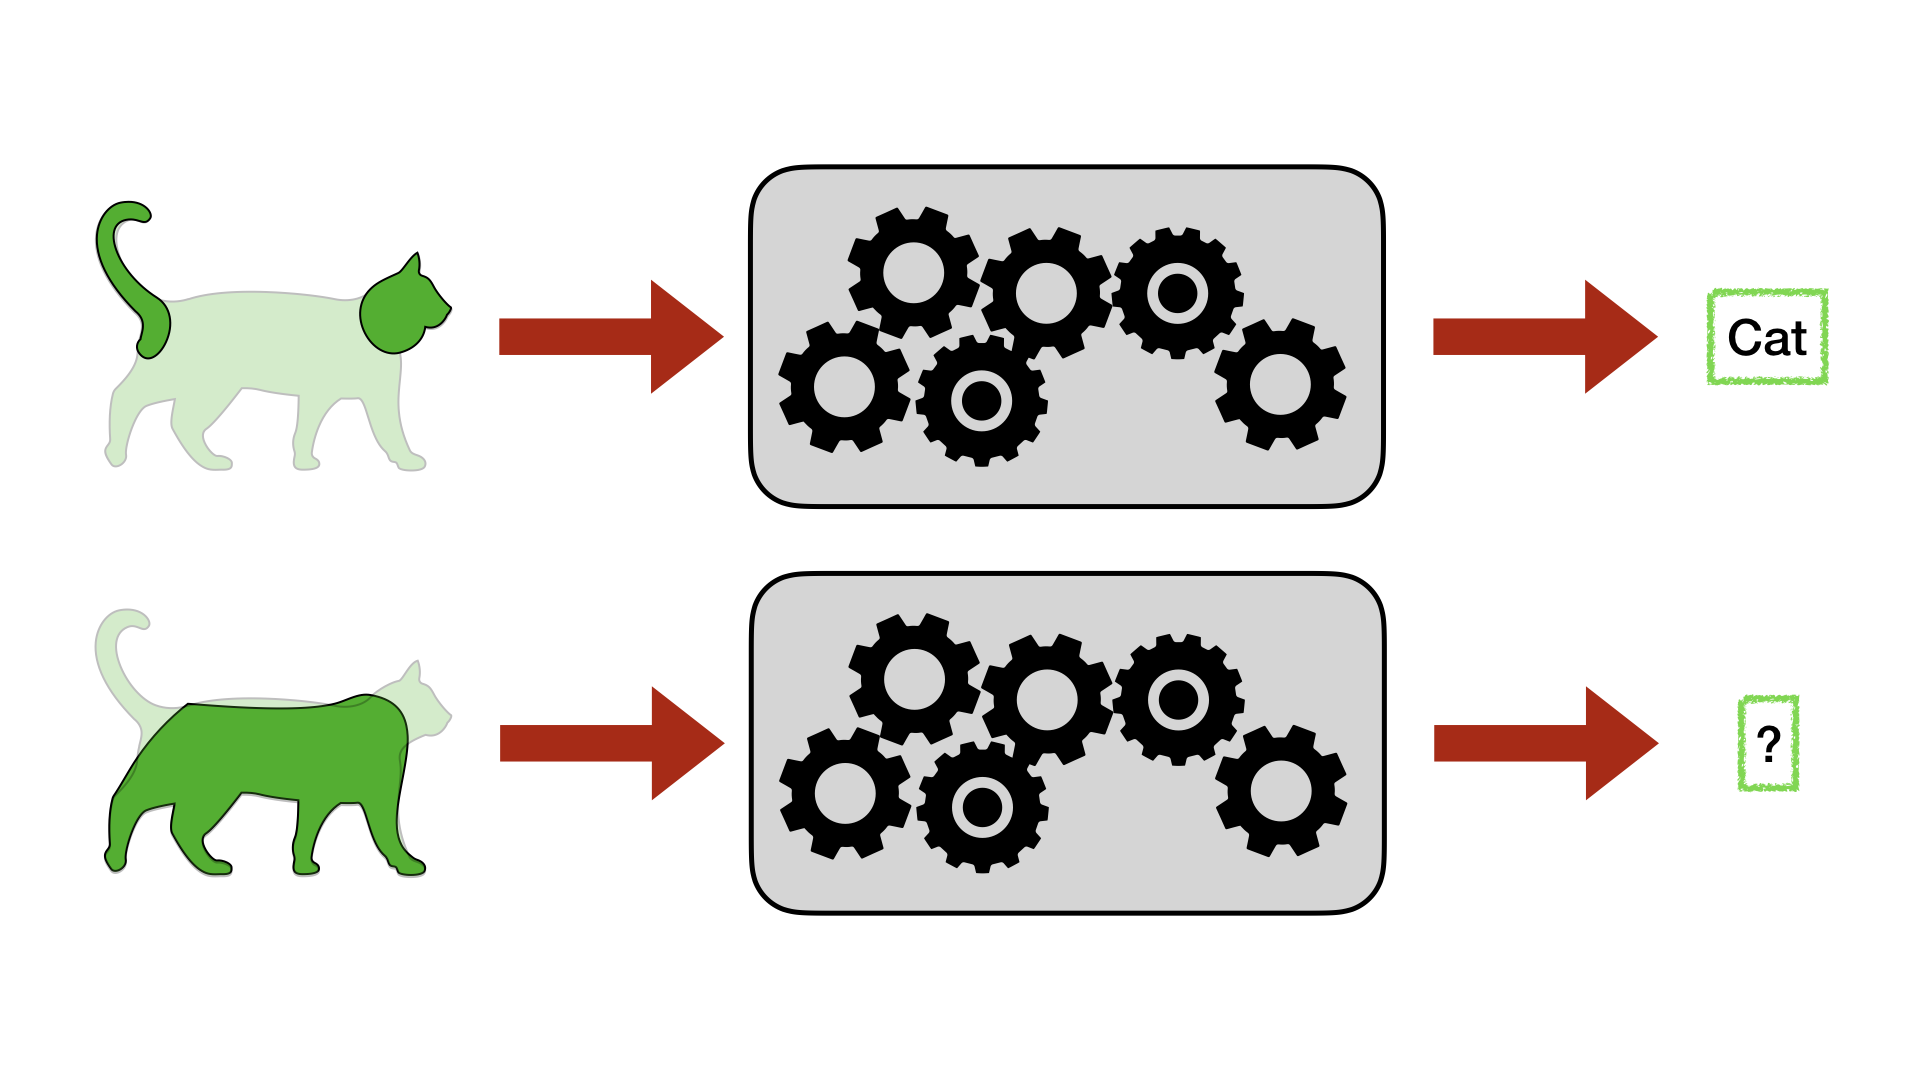
\includegraphics[trim={0 3cm 0 3cm},clip,width=0.9\textwidth]{diss/1_intro/figs/feat_select.png}
    \caption[Visualization of feature selection]{An example of identifying specific features important to the learning task.}
    \label{fig:feat_select}
\end{figure}
\paragraph{Feature Selection.} 
With more complex models $f$ compared to the linear case above, newer ``black-box'' methods have been developed for identifying important features. From the more pure statistics side, scan statistics~\citep{scanstat,scanstatlrt} allow for a structured ``scanning'' over the input space, skipping subsets unlikely to provide additional information for the measure of interest.
Further on the deep learning side, adaptations of sensitivity analysis, via noise addition and perturbations have found success~\citep{yeung2010sensitivity,zhang2015sensitivity}, alongside activation mapping~\citep{cam,selvaraju2017grad}.
These methods typically generate an analagous ``weighting'' over the input space, identifying features most salient for the specific task (Figure~\ref{fig:feat_select}).

\begin{figure}
    \centering
    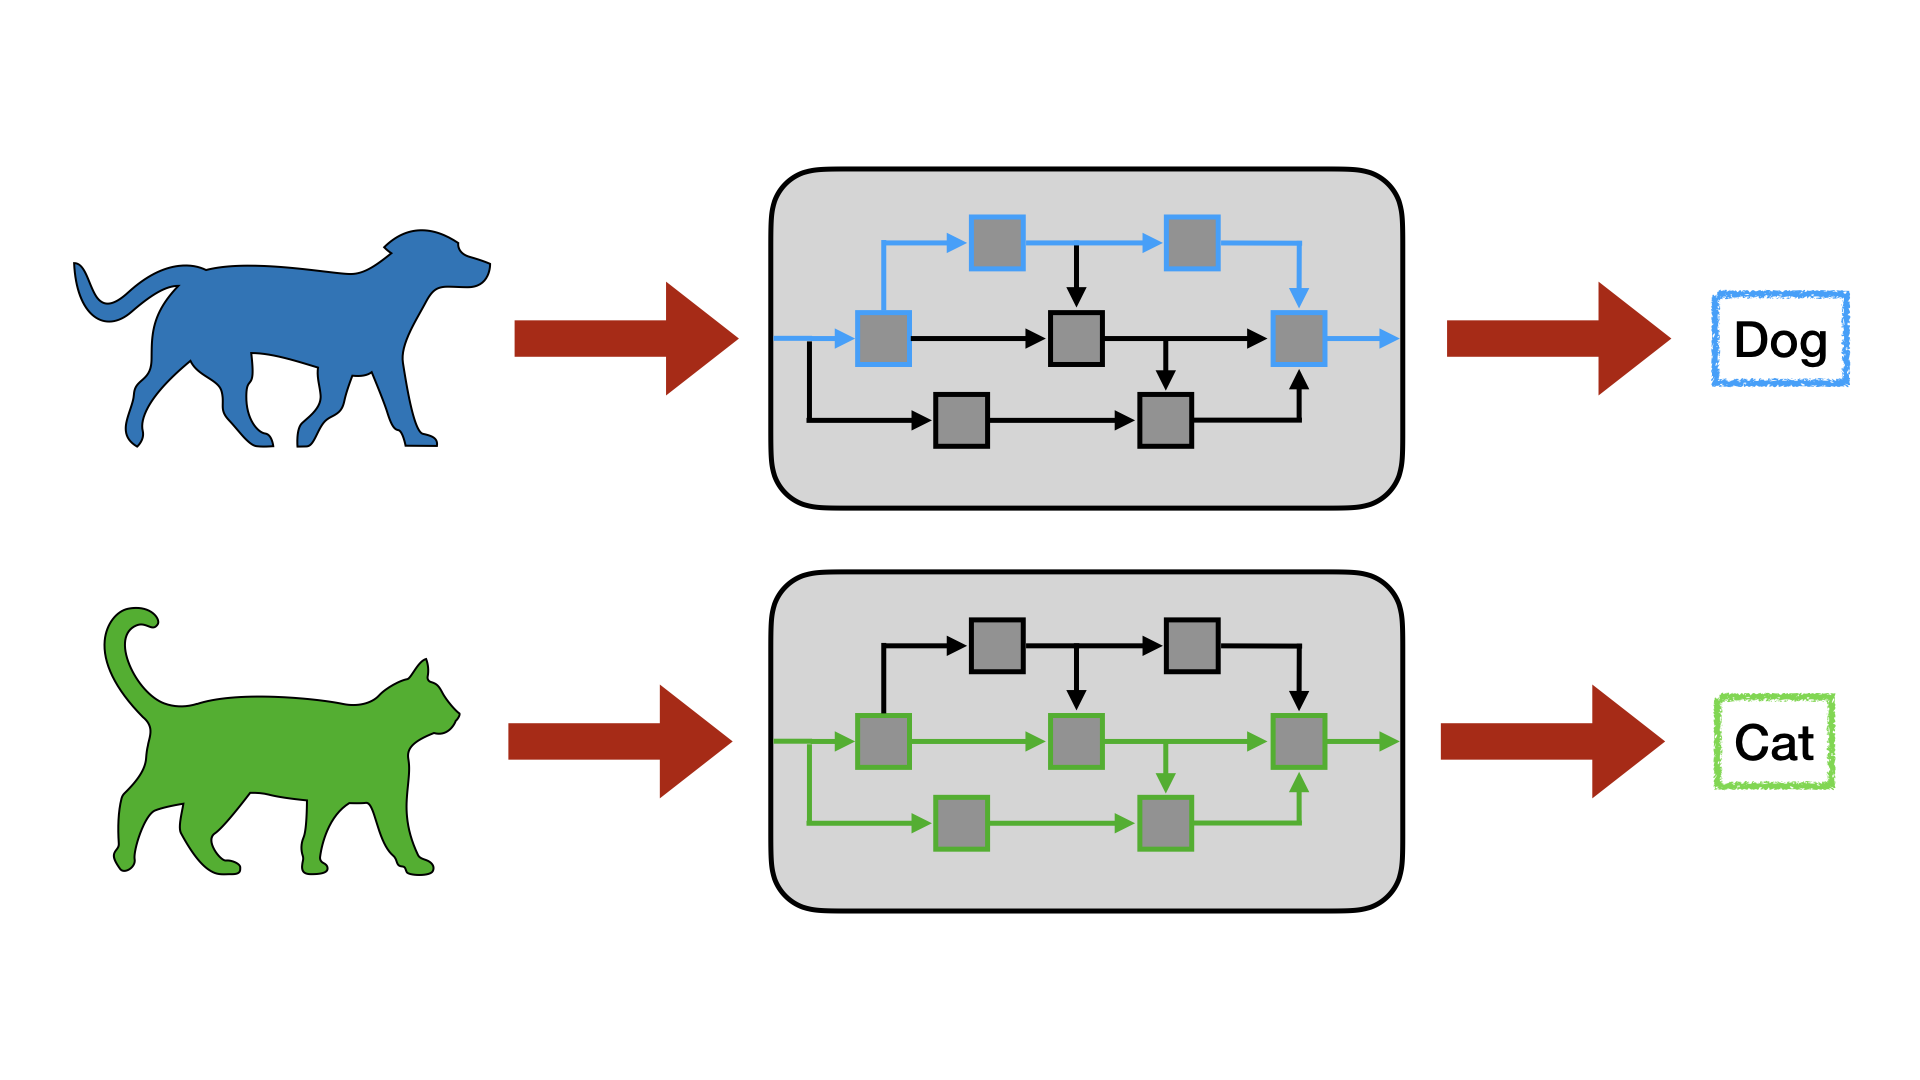
\includegraphics[trim={0 3cm 0 3cm},clip,width=0.9\textwidth]{diss/1_intro/figs/param_select.png}
    \caption[Visualization of parameter selection]{An example of identifying specific parameters important to the learning task.}
    \label{fig:param_select}
\end{figure}
\paragraph{Parameter Selection.} 
Selection in the model space generally takes two forms. First, as a prior, restriction, or assumption over the model space, and second, as a post-hoc method for an ``explainable'' proxy.
Regularization, sparsity, and gating methods are often used independent of the type or size of the model, to encourage the solution to fall within a specific region of the model space.
% In non-deep settings these methods come with strong theoretical guarantees. 
The theoretical underpinnings of these methods in deep learning are still being actively researched~\citep{hardt2016train,jacot2018neural,neyshabur2014search}, but the methods have nonetheless been effective in practice. 
On the post-hoc side, of particular interest are the parameters relevant to specific regions of the input space \textit{after} training (Figure~\ref{fig:param_select}). Here, recent analysis of deployed networks has shown this to be true~\citep{bau2017network,fong2018net2vec}, and current work continues to explore these network regions to aid in interpretability and explainability.

\paragraph{Sample Selection.} Many methods have been developed for outlier detection within training or testing sets~\citep{huang2020feature,ren2019likelihood} \textit{after} training, as well as methods for understanding sample influence~\citep{koh2017understanding,golatkar2020eternal,huang2020feature} . ``In-the-loop'' methods for accounting for ``outlierness'' behave similarly to accounting for group or individual fairness while training~\cite{mehrabi2021survey}. Unfortunately, once samples are identified in some manner, post-hoc adjustments to a trained model are generally very difficult. Recent work has focused on ``unlearning'', or removing a sample's influence on a model without retraining. If specific samples can be uniquely identified, performance and privacy reasons may require these specific interventions to reduce the ``influence'' of that sample subset.
\begin{figure}
    \centering
    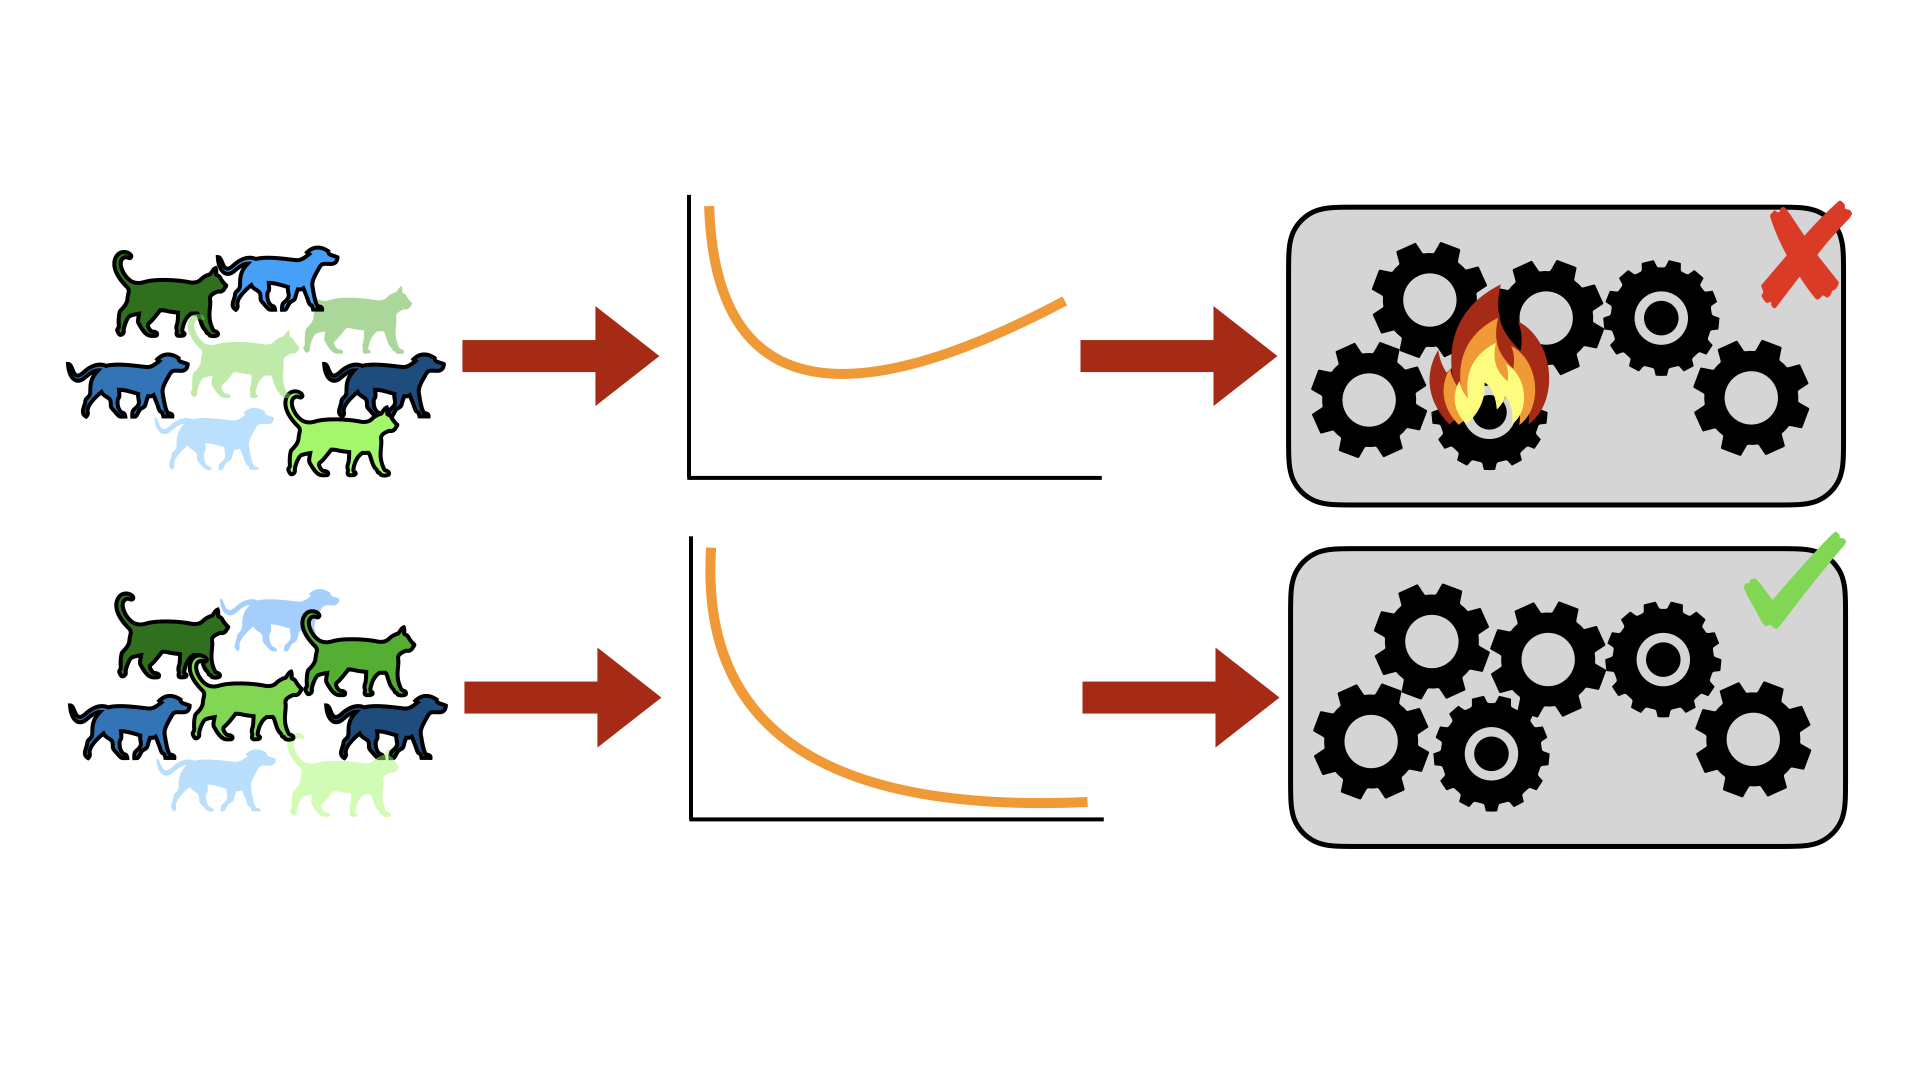
\includegraphics[trim={0 4.5cm 0 4cm},clip,width=0.9\textwidth]{diss/1_intro/figs/sample_select.png}
    \caption[Visualization of sample selection]{An example of identifying specific samples important to the learning task.}
    \label{fig:sample_select}
\end{figure}


\begin{mdframed}[style=MyFrame]
\textbf{ Thesis Goal: }
\em Identify, construct, and evaluate methods for \textbf{efficient} subset identification in modern machine learning feature, model, and input spaces.
\end{mdframed}

\section{A Few Motivating Examples}
Consider a traditional machine learning classification task in which we would like to predict whether an individual has a specific disease condition based on a medical resonance image (MRI) scan of their brain. Our input feature $x$ may consist of a 3D-array of values in $\RR^{\cI\times \cJ\times \cK}$ measuring some intensity of the imaging modality at each voxel, indexed by a tuple $(i,j,k) \in (\cI,\cJ,\cK)$.
Our outcome variable $y$ may simply be a binary label of whether the input scan has been labeled by a radiologist as one demonstrating typical disease characteristics.
Using an off the shelf 3D convolutional neural network with adjustments to match our input size, we can very quickly set up and train a system to predict disease presence with a high degree of accuracy.

\paragraph{Example 1.}
With a prediction for a specific scan, or predictions over a number of scans, we might be interested in identifying which regions of the brain are most important for diagnosis. These regions, $R \subset \cR:=\RR^{x\times y\times z}$, can be specific groups of pixels in the image that may correspond to known functional networks. Methods such as attention and class activation maps may work here, but there are a few issues. The number of samples available to learn a model is very small compared to the both the dimension of the input and the number of parameters in the model, i.e., $n \ll p$ and $n \ll d$. Thus it is very easy to overfit, and for areas of interest to be associated with intricacies of particular input data rather than true, real differences defined by the disease.

Furthermore, recent medical imaging studies have moved past simple difference detection: trends over time, and the ability to predict {\em future} disease development have by far become the setting of most interest.
Given an image of a healthy individual, is it possible to predict what their scan, or their future disease diagnosis, may be up to 10, 20, or more years in the future?
If a number of scans have been collected over some timeframe, can the \textit{trajectory} of the individuals' development be extrapolated to estimate progression?
As traditional models extended for temporal analysis grow in both size and complexity,
a number of subproblems explicitly related to model and input subspaces arise. In this thesis we address two such problems: \textbf{statistically rigorous identification of temporally evolving subsets}, and \textbf{characterizations of deep models that enable efficient training of recurrent models with large scale time-varying data}.
    
\paragraph{Example 2.}
With the rapid growth of AI and machine learning applications has come valid concerns regarding both guarantees of privacy.
Recent technology legislation has made the importance clear in all aspects of data use,
and particular projects and groups have demonstrated that machine learning is not independent of
this need \citep{Exposing}.
A new issue raised within this intersection is the ``right to be forgotten".
If a model has been trained with a particular users' data, 
they should have some recourse or right
to both remove their data from the training set,
and also know that the model has not learned from their data.
On the surface, this poses a significant problem for model builders
and organizations that spend large amounts
of time and resources in 
training deep learning models.

In the medical imaging example above this is especially important: with fewer samples it is more likely that information about any particular one could ``leak'', and the model's performance may degrade significantly as a relatively large percentage of it's training data is removed.
Thus tailored methods must be developed to ensure both privacy and performance, without requiring full retraining.
As we will see, 
\textbf{identification of model parameter subsets}
that are particularly important
for a particular sample's influence
in a model enables \textit{efficient machine unlearning}.

\paragraph{Example 3.}
From an alternative perspective, we may want to identify specific samples rather than have them specified a priori.
Traditionally a rigorous area of study under classical statistics, outlier detection and accounting have become a subfocus for many within the machine learning community as well \citep{golatkar2020eternal,golatkar2020forgetting,huang2020feature,ren2019likelihood}.
While subgroups of input samples may be outliers, it is more often the case that they represent known heterogeneity within the data. 
These differences may be marked using 
group information known a priori, and 
most learning tasks aim to learn tasks
in a \textit{subgroup-independent} manner.
In our disease prediction model above,
these groups could simply be stratified by the type of scanner used to acquire the image, but it could also
be a systematic difference correlated with some protected attribute. {\color{red} sentence about original brain atlas for registration being eurocentric}
This can directly lead to disparate performance and results on \textit{all} individuals outside of that group.
Optimization and regularization methods with this focus come under the umbrella of model fairness.
However, many existing methods do not scale well to larger models or as the number of subgroups grows, as is often the case when intersections of protected classes must be considered. Here we identify and construct a particular solution for \textbf{groupwise fairness that enables efficient in the loop fairness regularization}.

% What features are most important for prediction?
% Which samples were most important for my training?
% Can we understand when a model is certain or uncertain about its output?
% Are there layers in my network that have learned a particular subtask?
% Questions of robustness, bias, influence, fairness, and importance have become central questions to contemporary machine learning research \citep{doshi2017towards,mehrabi2021survey,amodei2016concrete}.
% machine learning, etc.

% Feature selection in the case of
% typical regression or classification 
% takes some form of learning parameters $\theta$ that allow for $\hat{y} = f_\theta(x)$ to be close to the true outcome of interest $y$.
% While forms of data $X := (x,y)$ may simply be continuous and real-valued, modern machine learning has greatly expanded formulations of the classical learning problem to include a wide variety of structured learning problems~\citep{nowozin2011structured}. 
% Consider the case when a high-dimensional input is used to predict an output with a highly-parametrized model. 
% Once learned, obvious questions arise as discussed above: are there specific low-dimensional spaces in either the input or the model space that are most important or necessary for the global learning problem of interest? Are there specific subspaces associated with particular subproblems of the global problem?
% The machine learning literature has come up with a number of ways to identify analogs of these spaces, 
% including extensions of sensitivity analysis to deep learning~\citep{yeung2010sensitivity,zhang2015sensitivity}, and constructing and identifying nonzero model subsets via particular model choices such as activations~\citep{selvaraju2017grad} and regularizers.
% In classical settings these are well understood: decision trees naturally provide ease of interpretibility via the information used to choose splits, and both linear and kernel support vector machines have been analyzed to provide for measures of sample importance via distances to the margin as well as feature importance via weights defining the learned hyperplane~\citep{Mitchell97}.
% Attention and saliency maps have emerged as popular new methods,
% given their ease of implementation and interpretation~\citep{sutskever2014sequence,vaswani2017attention,selvaraju2017grad}.
% By learning dimensions of a given input that are particularly important, either in a hard (binary) or soft (continuous weighting) manner, model builders are better able to understand and interpret what a model has learnt.
% The specific ideas of attention notwithstanding, many of these existing methods are far removed from traditional hypothesis testing frameworks.
% While some work has begun in this direction~\citep{tansey2018black},
% there remains a gap in direct identification of subsets and structures in these spaces that can be defined in statistically rigorous manners.

% \begin{figure}
%     \centering
%     \includegraphics[width=0.5\textwidth]{example-image-a}
%     \caption[A simple subset selection example]{\color{red} Identifying and selecting in MRIs, subset, sample, model ID.}
% \end{figure}

% \paragraph{A specific example.} 

% ------------------------------------------

% below here will be moved and arranged with the "selection" sections and here if relevant

% ------------------------------------------

% While attention can be directly applied to the network in order to identify ``hotspots" in the input space relating to the learned classification task, 
% given the high-dimensional nature of the input
% and the relatively small sample size 
% associated with medical imaging data, 
% it is very likely that an area of interest identified
% may be an intricacy of the training samples used rather than truly a region of disease signal.
% Class activation maps (CAMs) may be unclear, and can often associate with image artifacts unrelated to the scientific task~\citep{adebayo2018sanity}.
% Methods of generalization may help to increase confidence in identified regions, but statistical guarantees often remain out of reach.

% Furthermore, most recent problems associated with medical data have moved past simple difference detection: trends over time, and the ability to predict {\em future} disease development has by far become the setting of most interest.
% Given an image of a healthy individual, is it possible to predict what their scan, or their future disease diagnosis, may be up to 10, 20, or more years in the future?
% If a number of scans have been collected over some timeframe, can the \textit{trajectory} of the individuals' development be extrapolated to estimate progression?
% As traditional models extended for temporal analysis grow in both size and complexity,
% a number of subproblems explicitly related to model and input subspaces arise. Here we address two such problems: \textbf{statistically rigorous identification of temporally evolving subsets}, and \textbf{characterizations of deep models that enable efficient training of recurrent models with large scale time-varying data}.

% A sample's particular influence on model parameters aside, the identification of influential samples or subsets of samples more generally is of independent interest. 
% Traditionally a rigorous area of study under classical statistics, outlier detection and accounting have become a subfocus for many within the machine learning community as well \citep{golatkar2020eternal,golatkar2020forgetting,huang2020feature,ren2019likelihood}.
% While subgroups of input samples may be outliers, it is more often the case that they represent known heterogeneity within the data. 
% These differences are typically marked using 
% group information known a priori, and 
% most learning tasks aim to learn tasks
% in a \textit{subgroup-independent} manner.
% Optimization and regularization methods with this focus come under the umbrella of model fairness, and instead of identifying and boosting independences within the model or data, we aim to minimize them.
% However, many existing methods do not scale well as the number of subgroups grows, as is often the case when intersections of protected classes must be considered. In the sequel we identify and construct a particular solution for \textbf{groupwise fairness that enables efficient in the loop fairness regularization}.

\begin{mdframed}[style=MyFrame]
\em 
Here we focus our effort on identifying these important subsets of model, feature, and sample space for feature association, model size reduction, model unlearning, and, fairness. Specifically, taking advantage of both existing statistical and geometric methods, we develop new methods for localizing subsets in a range of settings from hypothesis testing to deep learning.
\end{mdframed}

\section{Thesis Scope and Contributions}

We explore the intersections of classical statistical and geometric constructions with modern machine learning methods. 
Figure~\ref{fig:scope} shows the overall scope projected along three axes: feature, parameter, and sample spaces.
Below we briefly introduce the main problems studied in this thesis.
\begin{figure}[!ht]
    \centering
    % \includegraphics[width=0.99\linewidth]{scope.pdf}
    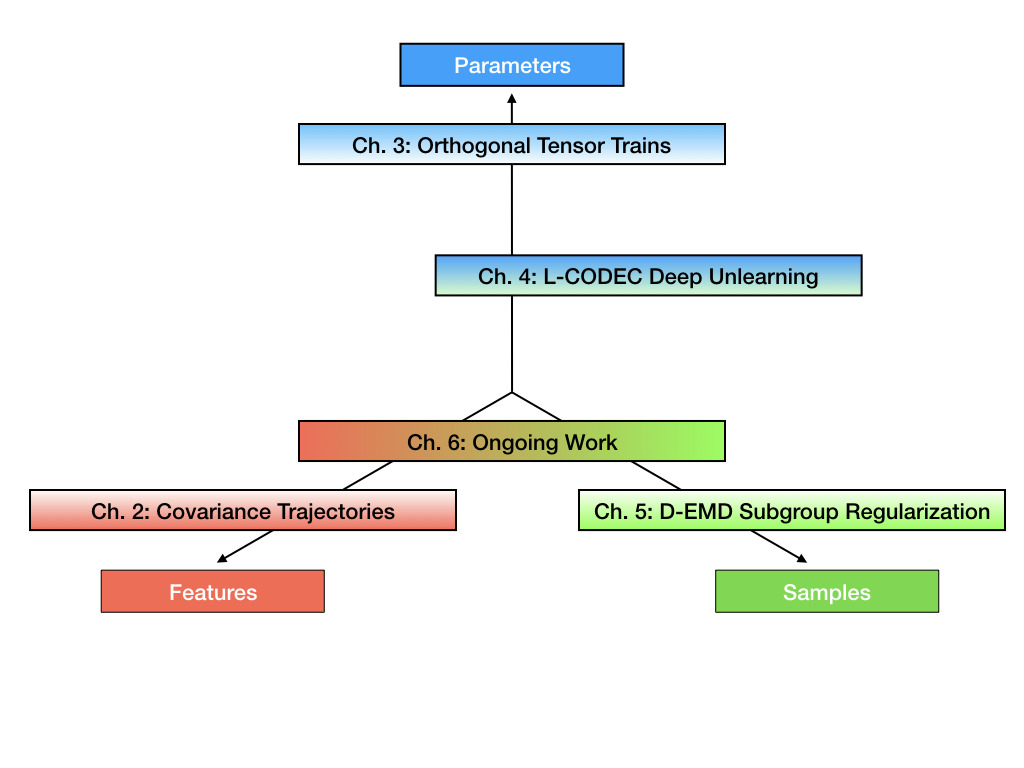
\includegraphics[width=0.95\linewidth]{diss/1_intro/figs/thesis_scope.png}
    \caption[Thesis Scope]{Thesis scope, projected over three representative axes. {\color{red} update chapter numbers shift by 1}}
    \label{fig:scope}
\end{figure}

\subsection{Second-Order Modeling and Group Difference Analysis over Time}

Recent results in coupled or temporal graphical models offer schemes for estimating the relationship structure 
between features when the data come from
related (but distinct) longitudinal sources. A novel application of these ideas is for analyzing group-level differences, i.e., in identifying if {\em trends} of estimated objects (e.g., 
covariance or precision matrices) are different across disparate conditions (e.g., gender or disease). Often, poor effect sizes make detecting the \textit{differential} signal 
over the {\em full} set of features difficult: for example, 
dependencies between only a {\em subset of features} may manifest differently across groups.
We first suggest
a parametric model 
for estimating trends in the space of $\SPD$ matrices as a function of one or more covariates.
We will then generalize scan statistics to graph structures, 
to search over distinct subsets of features (graph partitions) whose temporal dependency structure may show statistically 
significant group-wise differences.
We will theoretically analyze the Family Wise Error Rate (FWER) and bounds on Type 1 and Type 2 error. 
On a cohort of individuals with risk factors for Alzheimer's disease (but otherwise cognitively healthy), 
we 
find scientifically interesting 
group differences where the default analysis, 
i.e., models estimated on the full set of features, do not survive reasonable 
significance thresholds. 
% Preliminary work on this was published in \citep{covtraj}.


\subsection{Efficient Tensor Representations for Feasible Temporal Deep Learning}

Modern deep networks have proven to be very effective for analyzing real world images.
However, their application in medical imaging is still in its early stages,
primarily due to the large dimension of three-dimensional images, requiring enormous convolutional or fully connected layers --
if we treat an image (and not image patches) as a sample. 
These issues only compound when the focus moves towards longitudinal analysis
through recurrent structures, and when a point estimate of model parameters is insufficient 
in scientific applications where a reliability measure is necessary.
Using insights from differential geometry, 
we will adapt 
the tensor train decomposition to construct networks
with significantly fewer parameters,
allowing us to train powerful recurrent networks on whole brain image volumes. 
We analyze 
the \textit{orthogonal tensor train},
and demonstrate its ability to express a standard network layer both theoretically and empirically.
We 
demonstrate its ability to 
effectively reconstruct whole brain volumes
with faster convergence and stronger confidence intervals
compared to the standard tensor train decomposition. 
We provide code and show experiments on the ADNI dataset
using image sequences to regress on a cognition related outcome.
% Preliminary work on this was published in \citep{ott}.

\subsection{Practical Unlearning via Large-Scale Conditional Independence Testing}

%With AI systems extensively using personal %data for model training, 
Recent legislation has
led to interest in {\em machine unlearning}, i.e., removing specific training samples from a {\em predictive} model as if they never existed in the training dataset. 
Unlearning may also be required due to  corrupted/adversarial data or simply a user's updated privacy requirement.
For models which require no training ($k$-NN), 
simply deleting the closest original sample can be effective. 
%However, it is not clear how such approaches can be used to unlearn 
%models that contain rich information learned from the original data.
But this idea is inapplicable to models which learn richer 
representations.
%from data. 
%Recently, optimization-based unlearning estimators have been proposed, but 5their 
Recent ideas leveraging optimization-based updates
scale poorly with the model dimension $d$,  
due to 
inverting the Hessian of the loss function. %with an overall cost of $O(d^3)$ 
%is prohibitive.
We describe
a variant of a new conditional independence coefficient, 
L-CODEC, to identify a subset of the model parameters with the most semantic overlap on an individual sample level. 
Our approach completely avoids the need to invert a (possibly) huge matrix. 
By utilizing a Markov blanket selection, 
we find
that L-CODEC is also suitable for deep unlearning,
as well as other applications in vision.
Compared to alternatives, L-CODEC makes approximate unlearning possible 
in settings that would otherwise be infeasible, 
including vision models used for face recognition, 
person re-identification 
and NLP models that may require unlearning samples identified for exclusion.
% Preliminary work on this will appear in \citep{lcodec}.


\subsection{Reducing Subgroup Fairness via High Dimensional Earth Mover's Distances}

Optimal transport has recently emerged as a useful tool for machine learning through its connections with geometry, statistical machine learning, and through practical algorithms. Existing methods that leverage optimal transport often  regularize using  a Wasserstein metric or by computing barycenters, for example. %which are effective when distributions are continuous and known, or when measures of interest are discrete.
% Our formulation allows for a discretization of continuous measures that drop in directly to classical  formulations of the Earth Mover's Distance. 
We leverage optimal transport, except that we take advantage of a recently-introduced algorithm that computes a generalized earth mover's distance.
Not only is this algorithm computationally cheaper to compute compared to existing barycentric measures, but our method has the additional  advantage that gradients used for backpropagation can be directly read off of the forward pass computation, which leads to substantially faster model training.
We provide technical details about this new regularization term and its properties, 
and 
experimental demonstrations of improved training speed over existing Wasserstein-style methods.

{\color{red}
\subsection{Understanding Latent Spaces via Conditional Independences}

The final chapter of this thesis applies some of the tools developed above in the analysis of latent spaces in recent large scale models.
% In these studies, 
% we aim to identify conditionally independent features and subjects that are particularly important to the prediction and estimation of
% key disease outcomes,
% as a function of a number 
% of demographic, neuropsychological,
% genetic,
% and imaging data collected as 
% part of an ongoing consortium 
% to understand the progression
% of Alzheimer's disease in younger, 
% asymptomatic populations.
% In what follows we present
% exploratory analysis
% on a small, easily 
% digestible subset of the available data,
% that lays the foundation for
% further analysis.
}
% This work is the most forward looking, and aims to be a stepping stone toward a rigorous 

\section{Outline}
Chapter 2 covers the essential background necessary for the developments presented in the following chapters, including specifics of graphs and hypothesis testing, as well as relevant modern methods for learning and optimization.
In Chapters 3 through 7, we describe four perspectives to address subset identification.
Chapter 3 explores and focuses on the identification of feature subsets varying over time.
In Chapter 4 we describe a method of constraining the parameter space in a particular manner
that enables more efficient large scale neural networks.
Next, Chapter 5 provides a solution to the machine unlearning problem,
enabled through a particular conditional independence parameter selection scheme, vastly reducing network update costs.
Chapter 6 ends with a unique solution to subgroup fairness, 
where we take advantage of an efficient solution to
the $d$-dimensional earth mover's problem
to regularize large models when the number of subgroups can be large.
{\color{red} Chapter 7 describes future work, focused on applying a particular solution from Chapter 5 to understanding relationships among features in latent spaces learned by large generative models.}


%%%%%%%%%%%%% 
% Some old stuff

% Significant progress in the modern development of machine learning has
% been built upon connections and patterns identified across myriad
% interdisciplinary fields of study.
% Up through the mid 2000's, 
% many of these methods were inspired by and interested in 
% highly focused and constrained problems. 
% With a reasonably sized input domain, could a model of roughly equal size be used to
% predict some output?
% Linear regressors, decision trees, and support vector machines were all answers to these questions, with their own
% varying degrees of scaling and complexity.
% These methods necessitated carefully constructed formulations with specific restrictions to the learnable function class,
% enabling straightforward analysis 
% for provable performance guarantees 
% and easy identification of critical training samples and important input features.

% Contemporary machine learning, however, has a vastly different modus operandi. 
% Driven in large part by the exponential growth of available computation via Moore's Law, \textit{deep learning} has fallen squarely in the realm of \textbf{over-parameterized} models.
% With these overparametrizations and computation capacity, the typical learning questions posed as maximizing accuracy or reducing error have largely been addressed for even large scale problems.
% As such, complementary questions have led to subfields focusing on other performance measures, such as robustness, fairness, interpretability, and explainability.
% Many solutions to these questions end up looking back at answers found for the under- or non-parametrized settings.
% While nascent, these approaches 
% attempt to fill the gap between
% statistical and deep models to enable similar measures of sample influence, feature importance, and model analysis. 
% Most notable amongst these newer approaches is that of (Self)-Attention in Neural Networks \citep{sutskever2014sequence,vaswani2017attention}.
% Other proposals 
% end up looking back at the types of analysis typical of those more classical under-parametrized or nonparametrized methods.

% Not limited to previous developments in learning or computation theory, the arguably most valuable contributions toward the exponential reduction in model error can be attributed to influences and intuitions taken
% from biology, psychology, neuroscience, and even XXX \citep{srivastava, etc}.
% Perhaps one explanation as to why this phenomenon exists may be attributed to the way in which deep learning evolved. 
% The classical learning goal of function approximation lends itself nicely to a system which allows for arbitrary complexity via simple changes (e.g., addition of neural network layers). % Foundational works building on the original neural networks particularly have taken advantage of constraining this space of functions to search over: 
% the most seminal case being those of convolutional filters for imaging data. 
% While ``constraints" of this form have helped tremendously in model performance on modern vision and language machine learning tasks (GANs, Recurrent Networks, Residual Layers, Transformers, etc.), the ability to identify \textit{subsets} of important samples, input features, and model parameters has lagged significantly behind the development of these methods.
% Recently larger interest has been taken by the community to understand and interpret models with this view, only after extremely large and opaque models have become ubiquitous.
%This lag directly explains the more recent interest in developing methods for understanding and interpreting large scale machine learning models. % COVTRAJ
\chapter{Introduction} \label{chap:intro} 

Modern applications of machine learning in a broad range of industrial and consumer-facing systems have become ubiquitous.
Most interactions with daily technologies now intrinsically involve 
a request to some ``smart`` system in the ``cloud'', 
where those interactions range from
a request for map directions 
to simply loading a webpage.
Neural network models, and the recent advances of deep learning,
have enabled these systems that 
make such applications possible.
These models have achieved
human-level performance on learning tasks
including image classification~\citep{resnet,alexnet}, image segmentation~\citep{segmentation}, video analysis~\citep{zhang2016video}, text understanding and generation~\citep{bert,gpt}, and have slowly begun to solve more fundamental scientific problems such as protein folding~\citep{protein} drug discovery~\citep{drugdisc}, and medical diagnosis~\citep{diag}.
While this performance is largely attributed to model size,
the abundance of high quality training data
has equally contributed to real world performance,
enabling model training over millions of real world samples~\citep{imagenet,laion},
and potentially billions of synthetic samples via environment simulation~\citep{mcts}.

While deployment in some domains (recommender systems, object detection) may benefit almost unconditionally from this vastly expanded capability, rightful hesitancy has limited their widespread use in particular applications where impacts on individuals, people, or environments may be at stake.
These ``last mile'' concerns take a few forms.
% Because a completely accurate model is still out of reach, an important question that needs to be answered is: which inputs or individuals are being given incorrect outcomes, and why?
% maybe a sentence suggesting unlearning/removal
In mission critical applications such as medical diagnosis, 
the impact of an error can be extremely large,
even if a misprediction happens extremely infrequently.
Additionally, large scale model training and architecture search
can require exorbitant amounts of energy producing high emissions,
and their scale can limit market participants
to only large actors with vast existing resources.
The accessibility and effectiveness of these models can also vary significantly based on the training data, and disparate outcomes can be exacerbated by existing social inequity.

While existing human or ``natural'' systems that these models aim to assist are not perfect, 
our real world has developed norms and regulations that 
enable them to function.
A medical diagnosis might require a physician to explain what symptoms led them to that particular conclusion.
Energy metering and carbon taxes may be applied to limit
emissions.
Regulatory satisfaction may require 
analysis proving equal opportunity,
or that specific protected classes
are not used in decision making.
% Specifically, these can include ideas as simple as the Hippocratic Oath and medical malpractice insurance, to asking your doctor what symptoms lead them to a particular diagnosis.
These ideas are difficult to directly translate to automated machine learning systems,
but proxies have been identified that we can build upon.

These norms and regulations answer a number of questions we may also try to pose to our machine learning models.
What is the cost to learn this task?
What led to this particular outcome?
Why is this outcome different from another?
% We will explore how these questions can be formulated concretely. 

If the answer to these questions is negative or unknown,  follow-up questions all take an interesting form:
Can we learn a smaller model with similar performance? 
Can we identify the most important features? 
Which individuals or groups are being treated unfairly, and can we change that?
These questions ask us to identify a \textit{subset} of some relevant set, dependent on setting, and this identification is our focus here.

% Moving specifically to machine learning methods,
Taking a step back, let's take a look at a representative system. Figure~\ref{fig:dl} illustrates a typical learning pipeline. 
A dataset is collected and used to train a model, by minimizing the error over
those samples in the dataset (top).
A ``sample'' can be a single measured value, or it can
be a large, highly structured object with many ``features.''
The model is made up of some ``parameters'' that are 
tuned during training to learn a good predictor over the training dataset.
This model is then used to predict, or \textit{infer}, on new
data seen ``in the wild'' (bottom).
Our questions above are formally asking to identify \textit{subsets of these objects}: is a subset of the model parameters sufficient for learning? Which subset of the features are important for a prediction? Which subset of the dataset exhibit a specific attribute?
\begin{figure}
    \centering
    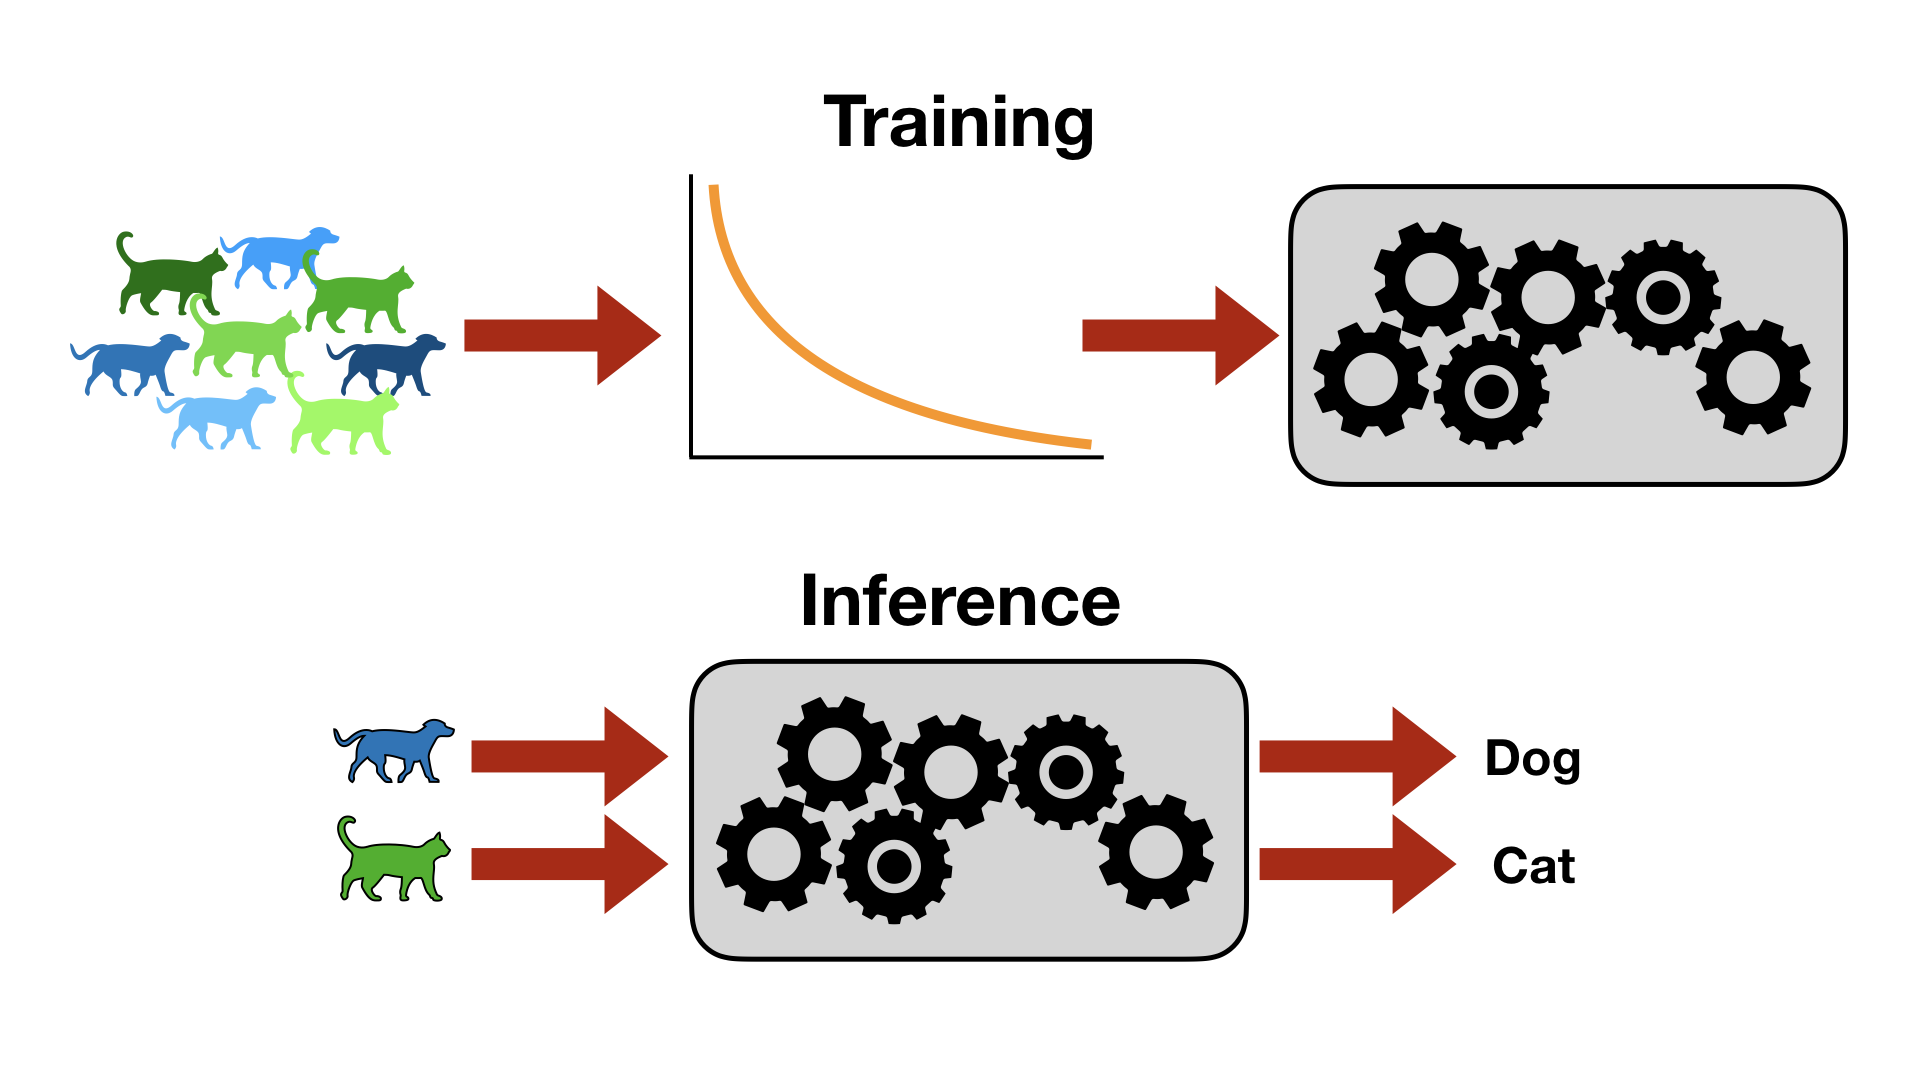
\includegraphics[trim={0 3cm 0 3cm},clip,width=0.95\textwidth]{diss/1_intro/figs/dl.png}
    \caption[Modern machine learning pipelines]{Machine learning training and inference visualization.}
    \label{fig:dl}
\end{figure}

% \textit{Explainability} can be seen as identifying important features of the input, as well as parts of the model (parameters) that ``light up`` for that input. \textit{Fairness} can be evaluated via measures over subsets of the data that correspond to specific groups. 

\begin{mdframed}[style=MyFrame]
\em 
\textbf{This thesis} focuses its main efforts on identifying these important subsets of model, feature, and sample space, to enable answering questions necessary for mainstream adoption of machine learning methods.
\end{mdframed}

% In this dissertation, we explore the sizes of these models, samples, and datasets, and 
% analyze under what situations 
% a smaller \textit{subset} of them may be sufficient or important
% for questions that run parallel to standard performance and accuracy measures.

Let us step a bit deeper into a basic illustrative example. In order to ease understanding, we can first begin with a basic formulation of learning methods, from which the questions above can take specific forms. 
Learning methods typically  try to identify a function mapping (model) that is able to complete a specific task at some high level of profficiency.
% In Figure~\ref{fig:dl}, a model is trained using examples of classification task (top), in order to accurately predict the class of a newly provided input (bottom).
% \begin{figure}
%     \centering
%     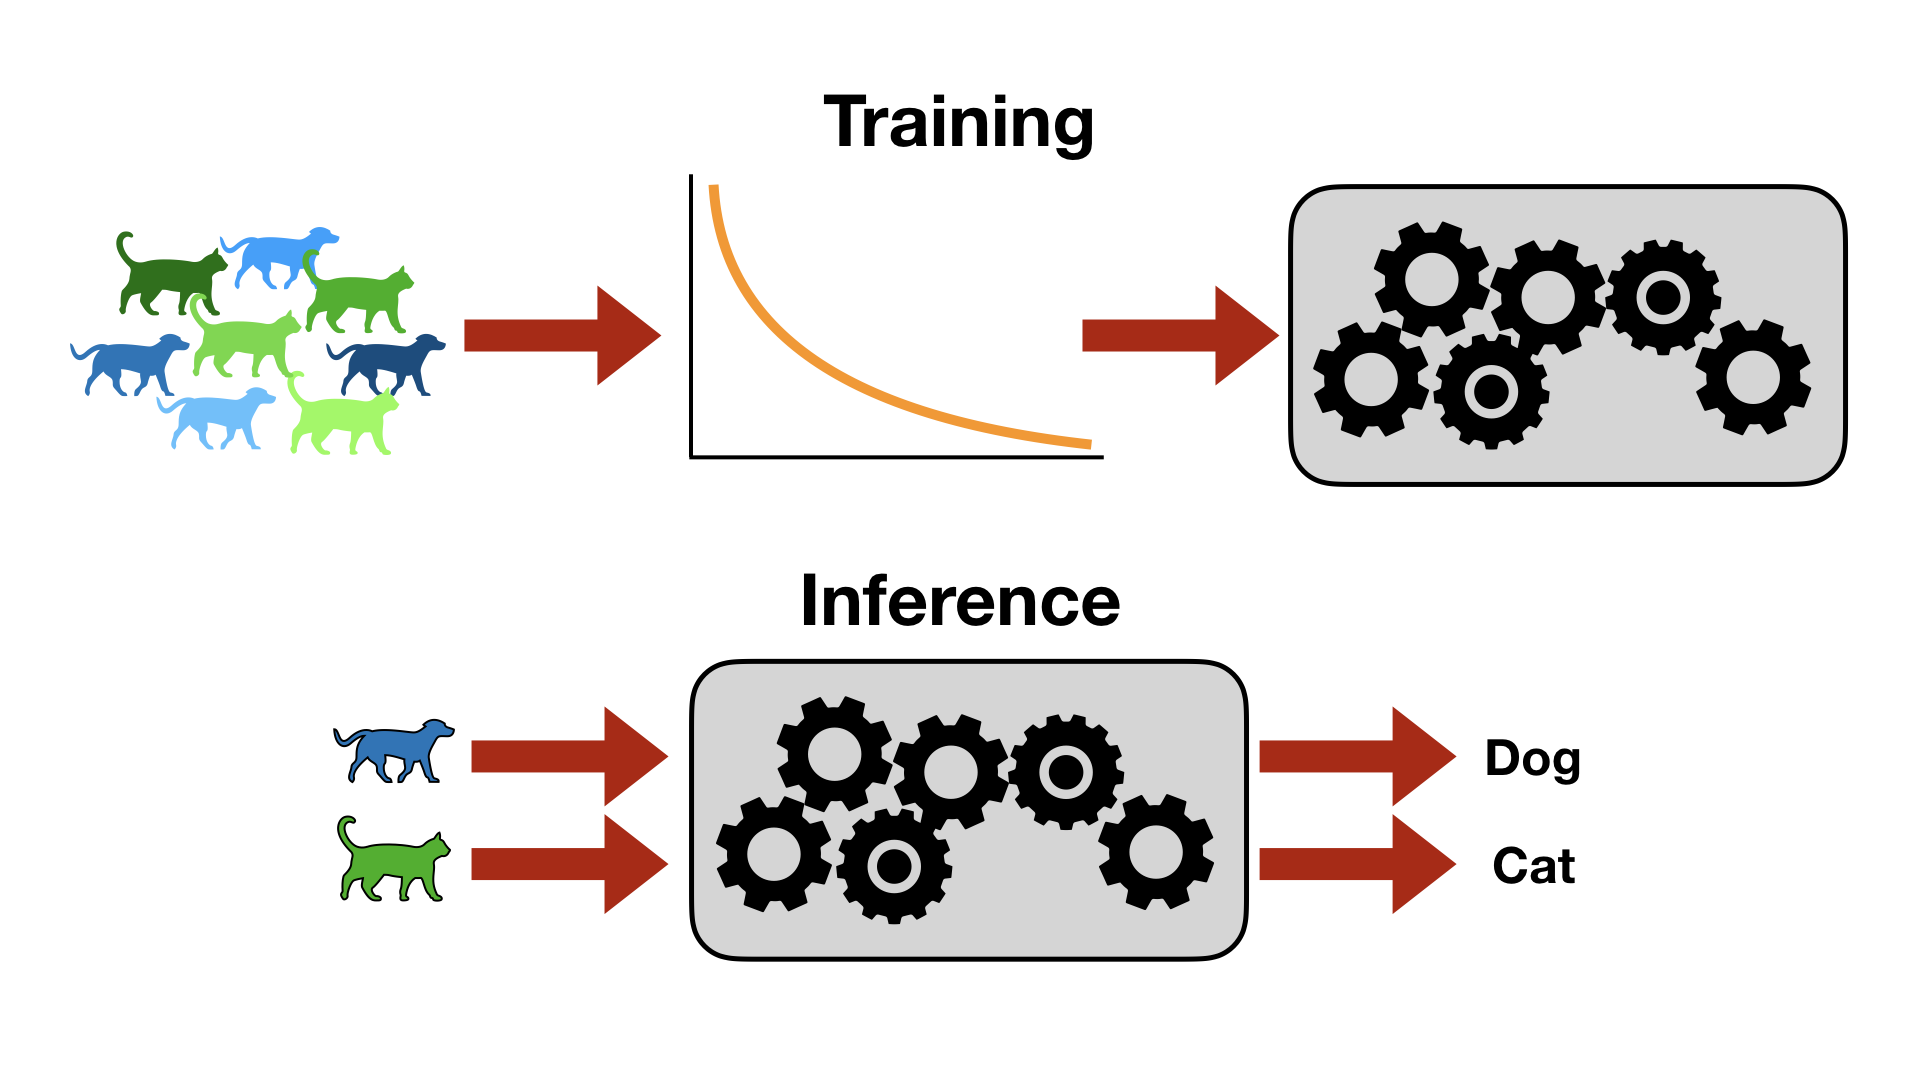
\includegraphics[trim={0 3cm 0 3cm},clip,width=0.95\textwidth]{diss/1_intro/figs/dl.png}
%     \caption[Modern machine learning pipelines]{Machine learning training and inference visualization.}
%     \label{fig:dl}
% \end{figure}
Say we have some dataset comprising of sample pairs $(x,y)$, where we wish to predict $y$ from $x$.
Our prediction, say $\hat{y}$, might be the output of some unknown function $f$ that we attempt to learn from training data. 
Let our approximation to this function be $\hat{y}:=\hat{f}(x)$.
This can take many forms, 
based on assumptions and prior information we may have on the relationships among the data. 
Consider the simple \textit{linear} case,
where we want to learn some parameter $w$ such that $y = w\cdot x$. 
Given $n$ sample pairs $(x_i,y_i)$ indexed by $i$, traditional statistics and optimization literature yield the following \textit{least squares} problem formulation, where we want to minimize the ``squared error'' between the observed values $y_i$ and the predicted $\hat{y}_i:= w\cdot x_i$:
\begin{align}\label{eq:lq}
\hat{f}:=\hat{w} = \mathop{\arg\min}_{w} \sum_{i=1}^n (y_i - w\cdot x_i)^2
\end{align}
This formulation expands without much change to a multi-dimensional form of the input $x$ and respectively, $w$: the canonical case where a number of features, or \textit{covariates} (e.g., symptoms), are used together to predict the outcome (e.g., diagnosis). 
If we are interested in which features of $x$ are important, we can look at the relative values of the learned ``weights'' $w$. In this simple setting, the importance of a feature (say $x^j$) can be exactly determined by the importance of the parameter ($w^j$).
A weight value far from zero may indicate that corresponding feature is important for diagnosis.
% If instead we are interested in which samples are most important, we can use existing methods for sample reweighting or methods that use standard assumptions to efficiently identify important subsets.

In this case and others, traditional statistical learning methods 
have been studied 
for many decades.
Linear regressors, decision trees, and support vector machines
have all been analyzed under these lenses.
% ,
% and as the modern machine learning community
% has returned to these questions recently,
% so has a renewed interest in their methods of analysis.
New research focuses
particularly on the differences
associated with moving from classical \textit{under-parametrized} models to
modern (deep) \textbf{over-parameterized} models: where
the model size vastly outnumbers the number
of input samples.
% , and may even be comparable to 
% the \textit{entire sample space.}
Methods for estimating the number of samples needed,
the time to learn a particular task,
and the generalization ability 
all require new perspectives in this regime.
While nascent, this research
attempts to fill the gap between
statistical and deep models to enable similar measures of sample influence, feature importance, and model understanding. 

\paragraph{A full picture.}
Let us expand our notation from the example above to consider this more general framing.
Consider a dataset $X:=\{x_i\}_{i=1}^n$ of size $n$ where each data point $x_i$ in the set $X$ is drawn from some underlying distribution over the domain $x_i \sim \cX^d$, 
with domain dimensionality (number of features) $d$.
A model $f$ is fit using a parametrization $\theta \in \Theta$,
with $\Theta$ the space of possible parametrizations (models) with some intrinsic dimension $p$. 
%While all three of these problems are closely related, they require different approaches. 
Generalizing the least squares``error measure'' from Eq.~\eqref{eq:lq} to an arbitrary \textit{loss} $\ell$, we have
\begin{align}\label{eq:learning}
    \hat{f}:=\hat{\theta} = \mathop{\arg\min}_{\theta\in\Theta} \sum_{x \in X} \ell(f_\theta(x_i))
\end{align}
From an analysis perspective, 
we might be interested in any one of 
(a) subsets of input features $\cC \subseteq \cX$ that are important for the downstream task,
(b) associating model subsets $\cP \subseteq \Theta$ with specific inputs or groups of inputs, or 
(c) subsets or subgroups of samples $S \subseteq \{X\}$ that are sufficient or representative of the entire dataset.

Crucially, an uninformed search for a subset is computationally infeasible. For a superset of size $n=|X|$, The set of all subsets is the power set, with a size of $2^{n}$! If an identification procedure requires looking over all of these and choosing a ``best'' one by some metric, the procedure will be limited to very small supersets.
Efficient methods have been developed in each of the three contexts above to avoid this exponential search.

\begin{figure}
    \centering
    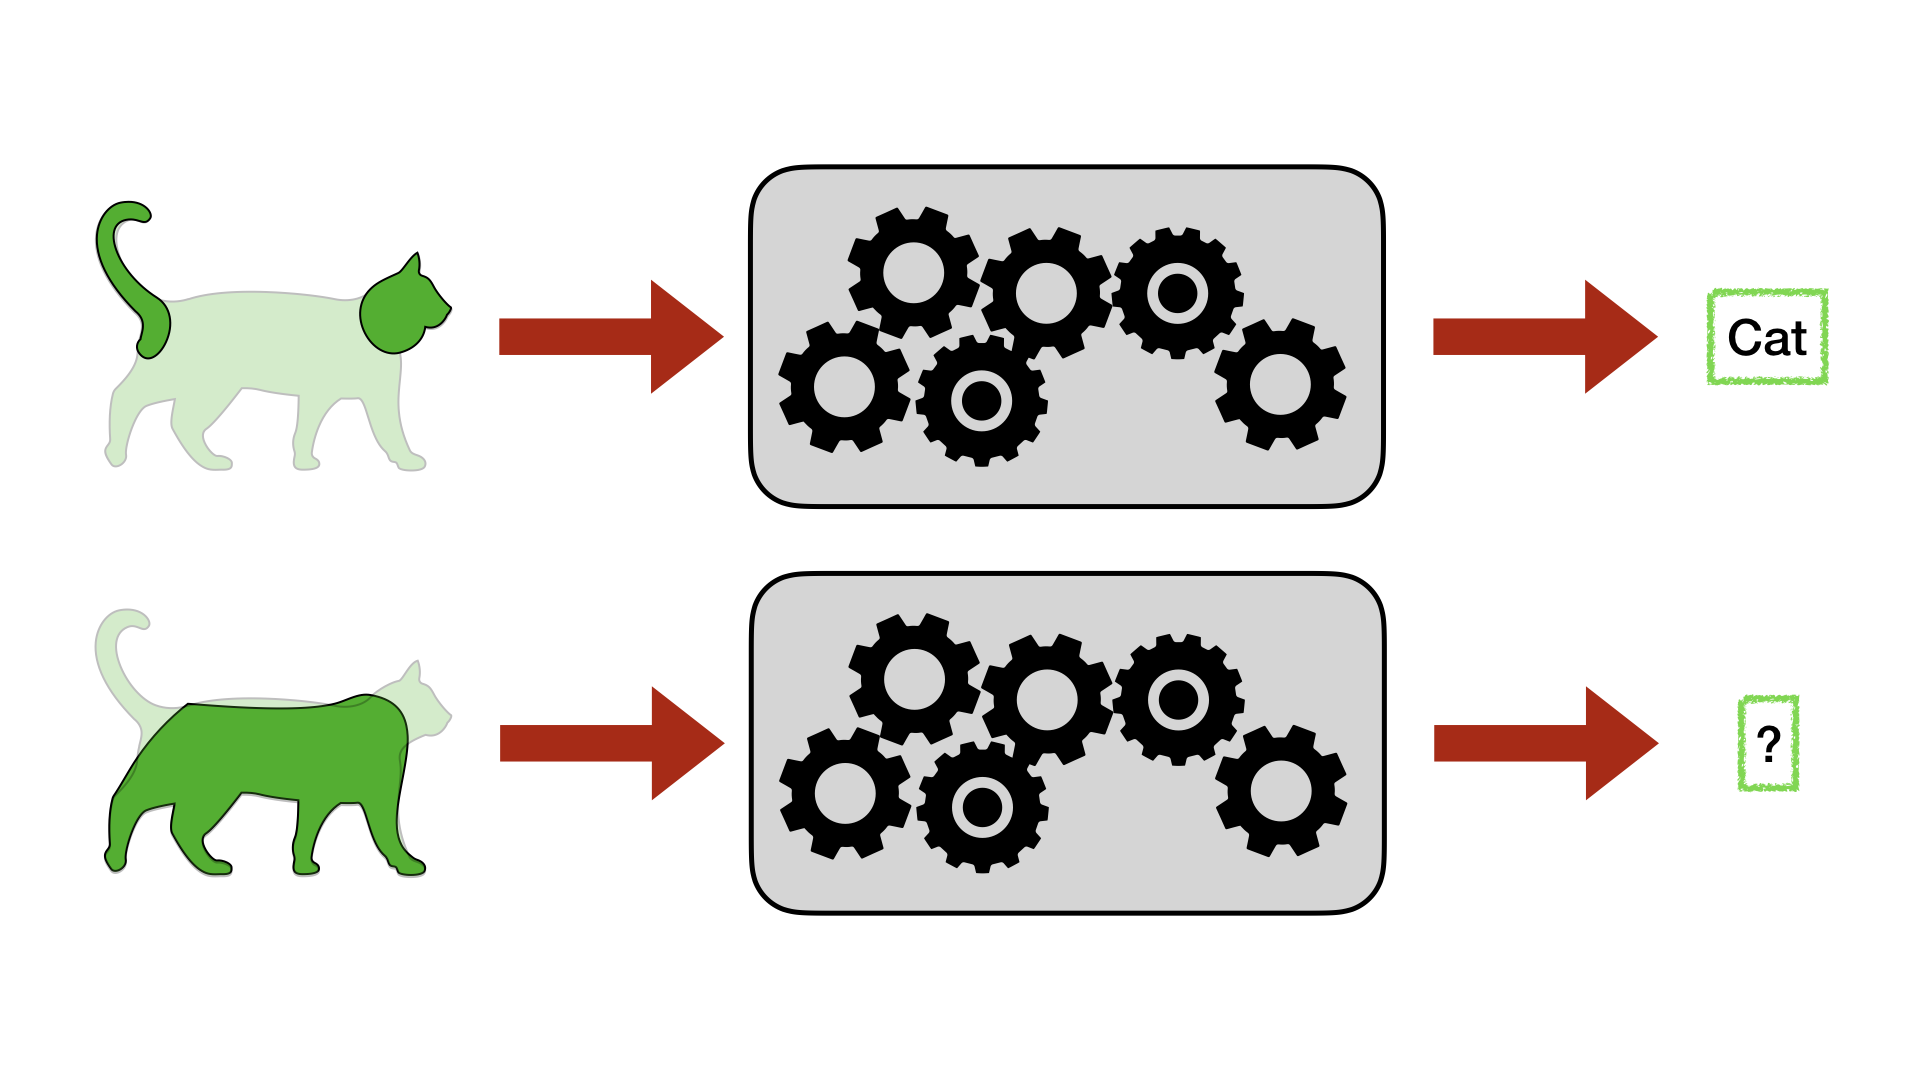
\includegraphics[trim={0 3cm 0 3cm},clip,width=0.9\textwidth]{diss/1_intro/figs/feat_select.png}
    \caption[Visualization of feature selection]{An example of identifying specific features important to the learning task.}
    \label{fig:feat_select}
\end{figure}
\paragraph{Feature Selection.} 
With more complex models $f$ compared to the linear case above, newer ``black-box'' methods have been developed for identifying important features. From the more pure statistics side, scan statistics~\citep{scanstat,scanstatlrt} allow for a structured ``scanning'' over the input space, skipping subsets unlikely to provide additional information for the measure of interest.
Further on the deep learning side, adaptations of sensitivity analysis, via noise addition and perturbations have found success~\citep{yeung2010sensitivity,zhang2015sensitivity}, alongside activation mapping~\citep{cam,selvaraju2017grad}.
These methods typically generate an analagous ``weighting'' over the input space, identifying features most salient for the specific task (Figure~\ref{fig:feat_select}).

\begin{figure}
    \centering
    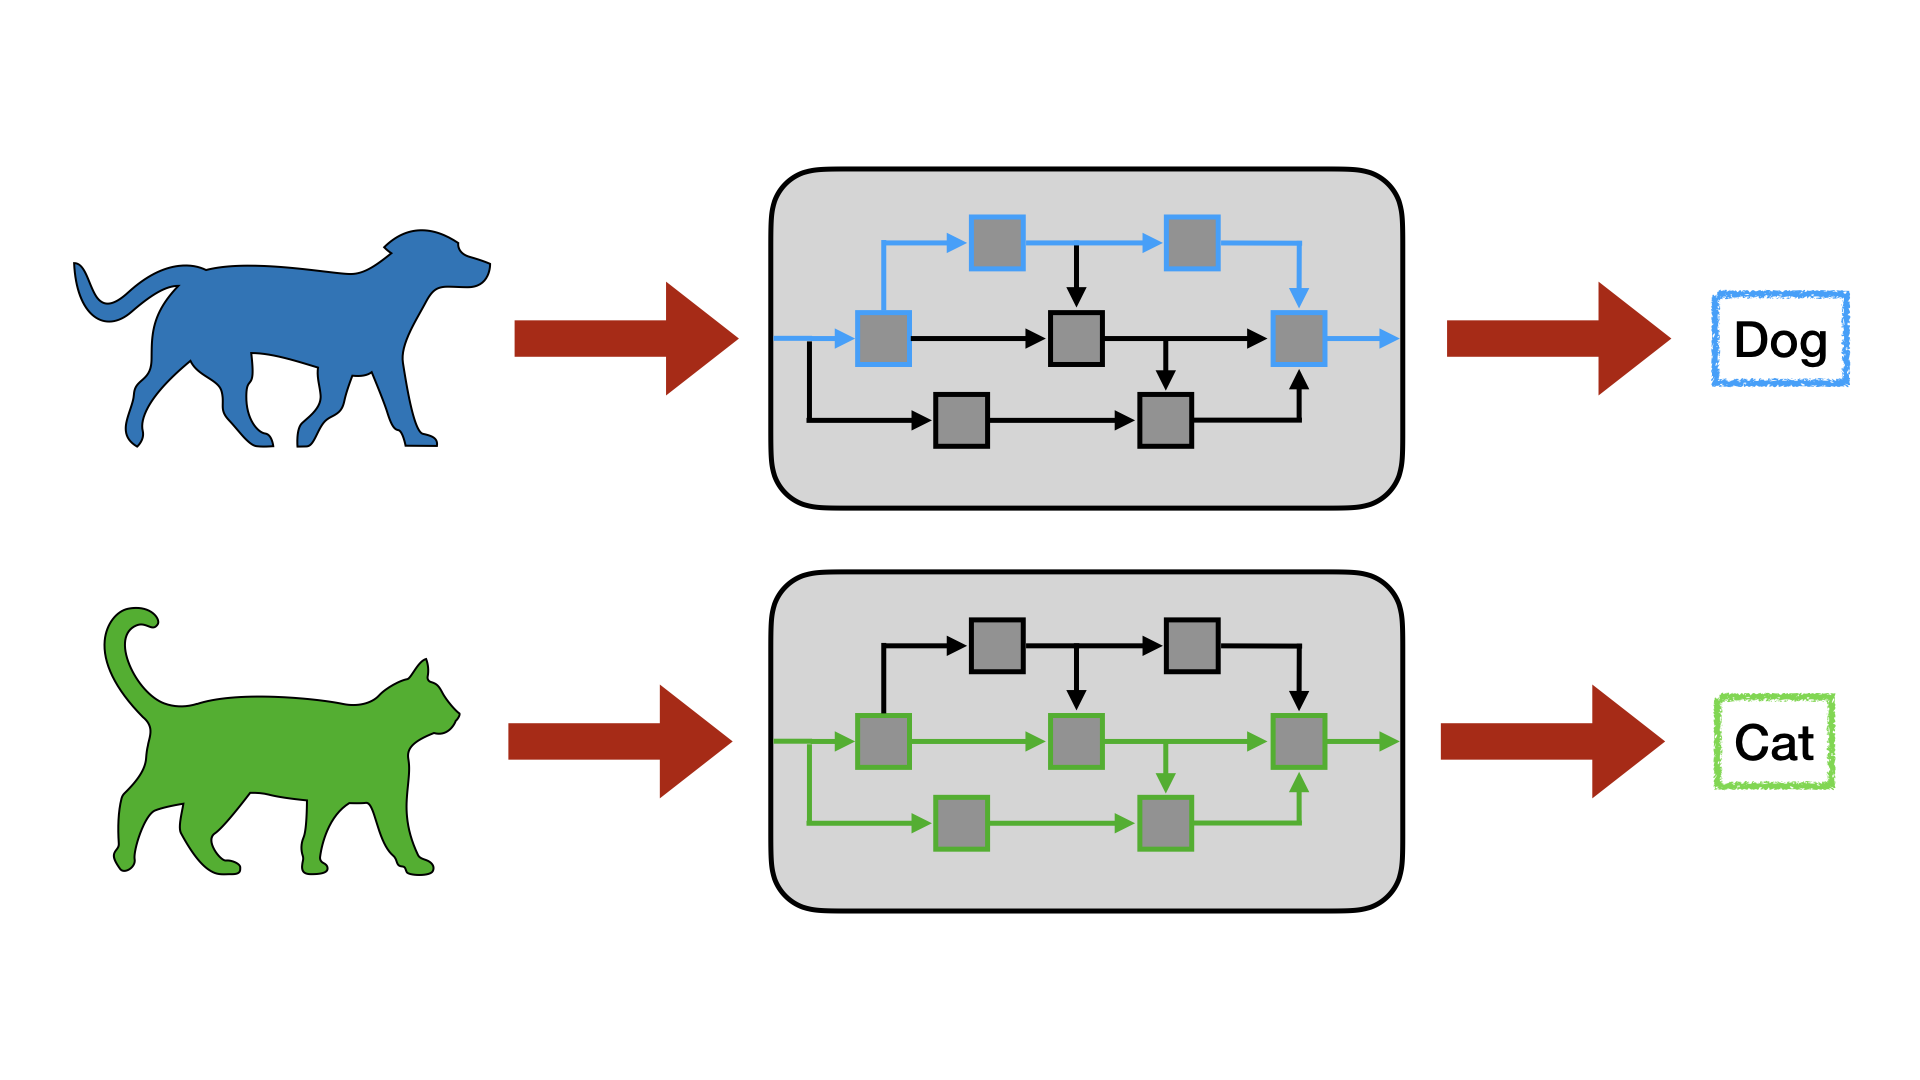
\includegraphics[trim={0 3cm 0 3cm},clip,width=0.9\textwidth]{diss/1_intro/figs/param_select.png}
    \caption[Visualization of parameter selection]{An example of identifying specific parameters important to the learning task.}
    \label{fig:param_select}
\end{figure}
\paragraph{Parameter Selection.} 
Selection in the model space generally takes two forms. First, as a prior, restriction, or assumption over the model space, and second, as a post-hoc method for an ``explainable'' proxy.
Regularization, sparsity, and gating methods are often used independent of the type or size of the model, to encourage the solution to fall within a specific region of the model space.
% In non-deep settings these methods come with strong theoretical guarantees. 
The theoretical underpinnings of these methods in deep learning are still being actively researched~\citep{hardt2016train,jacot2018neural,neyshabur2014search}, but the methods have nonetheless been effective in practice. 
On the post-hoc side, of particular interest are the parameters relevant to specific regions of the input space \textit{after} training (Figure~\ref{fig:param_select}). Here, recent analysis of deployed networks has shown this to be true~\citep{bau2017network,fong2018net2vec}, and current work continues to explore these network regions to aid in interpretability and explainability.

\paragraph{Sample Selection.} Many methods have been developed for outlier detection within training or testing sets~\citep{huang2020feature,ren2019likelihood} \textit{after} training, as well as methods for understanding sample influence~\citep{koh2017understanding,golatkar2020eternal,huang2020feature} . ``In-the-loop'' methods for accounting for ``outlierness'' behave similarly to accounting for group or individual fairness while training~\cite{mehrabi2021survey}. Unfortunately, once samples are identified in some manner, post-hoc adjustments to a trained model are generally very difficult. Recent work has focused on ``unlearning'', or removing a sample's influence on a model without retraining. If specific samples can be uniquely identified, performance and privacy reasons may require these specific interventions to reduce the ``influence'' of that sample subset.
\begin{figure}
    \centering
    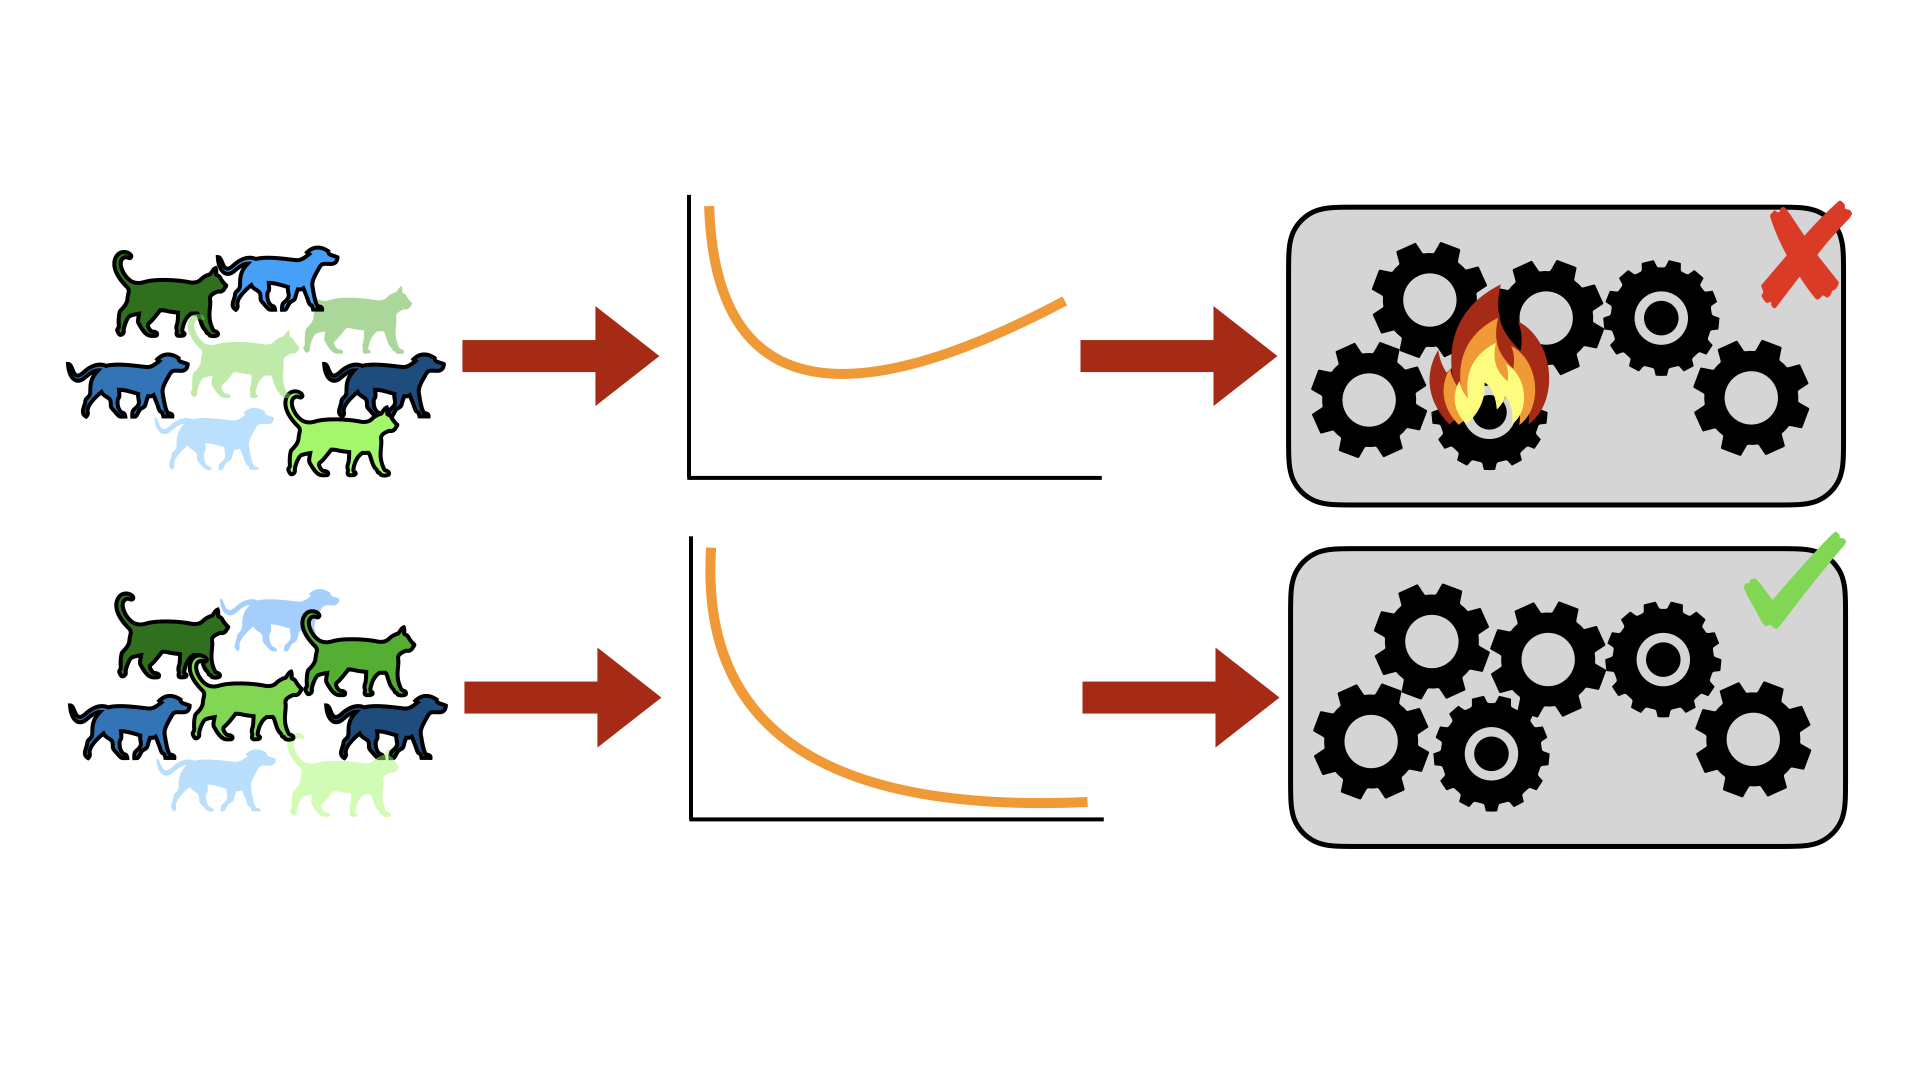
\includegraphics[trim={0 4.5cm 0 4cm},clip,width=0.9\textwidth]{diss/1_intro/figs/sample_select.png}
    \caption[Visualization of sample selection]{An example of identifying specific samples important to the learning task.}
    \label{fig:sample_select}
\end{figure}


\begin{mdframed}[style=MyFrame]
\textbf{ Thesis Goal: }
\em Identify, construct, and evaluate methods for \textbf{efficient} subset identification in modern machine learning feature, model, and input spaces.
\end{mdframed}

\section{A Few Motivating Examples}
Consider a traditional machine learning classification task in which we would like to predict whether an individual has a specific disease condition based on a medical resonance image (MRI) scan of their brain. Our input feature $x$ may consist of a 3D-array of values in $\RR^{\cI\times \cJ\times \cK}$ measuring some intensity of the imaging modality at each voxel, indexed by a tuple $(i,j,k) \in (\cI,\cJ,\cK)$.
Our outcome variable $y$ may simply be a binary label of whether the input scan has been labeled by a radiologist as one demonstrating typical disease characteristics.
Using an off the shelf 3D convolutional neural network with adjustments to match our input size, we can very quickly set up and train a system to predict disease presence with a high degree of accuracy.

\paragraph{Example 1.}
With a prediction for a specific scan, or predictions over a number of scans, we might be interested in identifying which regions of the brain are most important for diagnosis. These regions, $R \subset \cR:=\RR^{x\times y\times z}$, can be specific groups of pixels in the image that may correspond to known functional networks. Methods such as attention and class activation maps may work here, but there are a few issues. The number of samples available to learn a model is very small compared to the both the dimension of the input and the number of parameters in the model, i.e., $n \ll p$ and $n \ll d$. Thus it is very easy to overfit, and for areas of interest to be associated with intricacies of particular input data rather than true, real differences defined by the disease.

Furthermore, recent medical imaging studies have moved past simple difference detection: trends over time, and the ability to predict {\em future} disease development have by far become the setting of most interest.
Given an image of a healthy individual, is it possible to predict what their scan, or their future disease diagnosis, may be up to 10, 20, or more years in the future?
If a number of scans have been collected over some timeframe, can the \textit{trajectory} of the individuals' development be extrapolated to estimate progression?
As traditional models extended for temporal analysis grow in both size and complexity,
a number of subproblems explicitly related to model and input subspaces arise. In this thesis we address two such problems: \textbf{statistically rigorous identification of temporally evolving subsets}, and \textbf{characterizations of deep models that enable efficient training of recurrent models with large scale time-varying data}.
    
\paragraph{Example 2.}
With the rapid growth of AI and machine learning applications has come valid concerns regarding both guarantees of privacy.
Recent technology legislation has made the importance clear in all aspects of data use,
and particular projects and groups have demonstrated that machine learning is not independent of
this need \citep{Exposing}.
A new issue raised within this intersection is the ``right to be forgotten".
If a model has been trained with a particular users' data, 
they should have some recourse or right
to both remove their data from the training set,
and also know that the model has not learned from their data.
On the surface, this poses a significant problem for model builders
and organizations that spend large amounts
of time and resources in 
training deep learning models.

In the medical imaging example above this is especially important: with fewer samples it is more likely that information about any particular one could ``leak'', and the model's performance may degrade significantly as a relatively large percentage of it's training data is removed.
Thus tailored methods must be developed to ensure both privacy and performance, without requiring full retraining.
As we will see, 
\textbf{identification of model parameter subsets}
that are particularly important
for a particular sample's influence
in a model enables \textit{efficient machine unlearning}.

\paragraph{Example 3.}
From an alternative perspective, we may want to identify specific samples rather than have them specified a priori.
Traditionally a rigorous area of study under classical statistics, outlier detection and accounting have become a subfocus for many within the machine learning community as well \citep{golatkar2020eternal,golatkar2020forgetting,huang2020feature,ren2019likelihood}.
While subgroups of input samples may be outliers, it is more often the case that they represent known heterogeneity within the data. 
These differences may be marked using 
group information known a priori, and 
most learning tasks aim to learn tasks
in a \textit{subgroup-independent} manner.
In our disease prediction model above,
these groups could simply be stratified by the type of scanner used to acquire the image, but it could also
be a systematic difference correlated with some protected attribute. {\color{red} sentence about original brain atlas for registration being eurocentric}
This can directly lead to disparate performance and results on \textit{all} individuals outside of that group.
Optimization and regularization methods with this focus come under the umbrella of model fairness.
However, many existing methods do not scale well to larger models or as the number of subgroups grows, as is often the case when intersections of protected classes must be considered. Here we identify and construct a particular solution for \textbf{groupwise fairness that enables efficient in the loop fairness regularization}.

% What features are most important for prediction?
% Which samples were most important for my training?
% Can we understand when a model is certain or uncertain about its output?
% Are there layers in my network that have learned a particular subtask?
% Questions of robustness, bias, influence, fairness, and importance have become central questions to contemporary machine learning research \citep{doshi2017towards,mehrabi2021survey,amodei2016concrete}.
% machine learning, etc.

% Feature selection in the case of
% typical regression or classification 
% takes some form of learning parameters $\theta$ that allow for $\hat{y} = f_\theta(x)$ to be close to the true outcome of interest $y$.
% While forms of data $X := (x,y)$ may simply be continuous and real-valued, modern machine learning has greatly expanded formulations of the classical learning problem to include a wide variety of structured learning problems~\citep{nowozin2011structured}. 
% Consider the case when a high-dimensional input is used to predict an output with a highly-parametrized model. 
% Once learned, obvious questions arise as discussed above: are there specific low-dimensional spaces in either the input or the model space that are most important or necessary for the global learning problem of interest? Are there specific subspaces associated with particular subproblems of the global problem?
% The machine learning literature has come up with a number of ways to identify analogs of these spaces, 
% including extensions of sensitivity analysis to deep learning~\citep{yeung2010sensitivity,zhang2015sensitivity}, and constructing and identifying nonzero model subsets via particular model choices such as activations~\citep{selvaraju2017grad} and regularizers.
% In classical settings these are well understood: decision trees naturally provide ease of interpretibility via the information used to choose splits, and both linear and kernel support vector machines have been analyzed to provide for measures of sample importance via distances to the margin as well as feature importance via weights defining the learned hyperplane~\citep{Mitchell97}.
% Attention and saliency maps have emerged as popular new methods,
% given their ease of implementation and interpretation~\citep{sutskever2014sequence,vaswani2017attention,selvaraju2017grad}.
% By learning dimensions of a given input that are particularly important, either in a hard (binary) or soft (continuous weighting) manner, model builders are better able to understand and interpret what a model has learnt.
% The specific ideas of attention notwithstanding, many of these existing methods are far removed from traditional hypothesis testing frameworks.
% While some work has begun in this direction~\citep{tansey2018black},
% there remains a gap in direct identification of subsets and structures in these spaces that can be defined in statistically rigorous manners.

% \begin{figure}
%     \centering
%     \includegraphics[width=0.5\textwidth]{example-image-a}
%     \caption[A simple subset selection example]{\color{red} Identifying and selecting in MRIs, subset, sample, model ID.}
% \end{figure}

% \paragraph{A specific example.} 

% ------------------------------------------

% below here will be moved and arranged with the "selection" sections and here if relevant

% ------------------------------------------

% While attention can be directly applied to the network in order to identify ``hotspots" in the input space relating to the learned classification task, 
% given the high-dimensional nature of the input
% and the relatively small sample size 
% associated with medical imaging data, 
% it is very likely that an area of interest identified
% may be an intricacy of the training samples used rather than truly a region of disease signal.
% Class activation maps (CAMs) may be unclear, and can often associate with image artifacts unrelated to the scientific task~\citep{adebayo2018sanity}.
% Methods of generalization may help to increase confidence in identified regions, but statistical guarantees often remain out of reach.

% Furthermore, most recent problems associated with medical data have moved past simple difference detection: trends over time, and the ability to predict {\em future} disease development has by far become the setting of most interest.
% Given an image of a healthy individual, is it possible to predict what their scan, or their future disease diagnosis, may be up to 10, 20, or more years in the future?
% If a number of scans have been collected over some timeframe, can the \textit{trajectory} of the individuals' development be extrapolated to estimate progression?
% As traditional models extended for temporal analysis grow in both size and complexity,
% a number of subproblems explicitly related to model and input subspaces arise. Here we address two such problems: \textbf{statistically rigorous identification of temporally evolving subsets}, and \textbf{characterizations of deep models that enable efficient training of recurrent models with large scale time-varying data}.

% A sample's particular influence on model parameters aside, the identification of influential samples or subsets of samples more generally is of independent interest. 
% Traditionally a rigorous area of study under classical statistics, outlier detection and accounting have become a subfocus for many within the machine learning community as well \citep{golatkar2020eternal,golatkar2020forgetting,huang2020feature,ren2019likelihood}.
% While subgroups of input samples may be outliers, it is more often the case that they represent known heterogeneity within the data. 
% These differences are typically marked using 
% group information known a priori, and 
% most learning tasks aim to learn tasks
% in a \textit{subgroup-independent} manner.
% Optimization and regularization methods with this focus come under the umbrella of model fairness, and instead of identifying and boosting independences within the model or data, we aim to minimize them.
% However, many existing methods do not scale well as the number of subgroups grows, as is often the case when intersections of protected classes must be considered. In the sequel we identify and construct a particular solution for \textbf{groupwise fairness that enables efficient in the loop fairness regularization}.

\begin{mdframed}[style=MyFrame]
\em 
Here we focus our effort on identifying these important subsets of model, feature, and sample space for feature association, model size reduction, model unlearning, and, fairness. Specifically, taking advantage of both existing statistical and geometric methods, we develop new methods for localizing subsets in a range of settings from hypothesis testing to deep learning.
\end{mdframed}

\section{Thesis Scope and Contributions}

We explore the intersections of classical statistical and geometric constructions with modern machine learning methods. 
Figure~\ref{fig:scope} shows the overall scope projected along three axes: feature, parameter, and sample spaces.
Below we briefly introduce the main problems studied in this thesis.
\begin{figure}[!ht]
    \centering
    % \includegraphics[width=0.99\linewidth]{scope.pdf}
    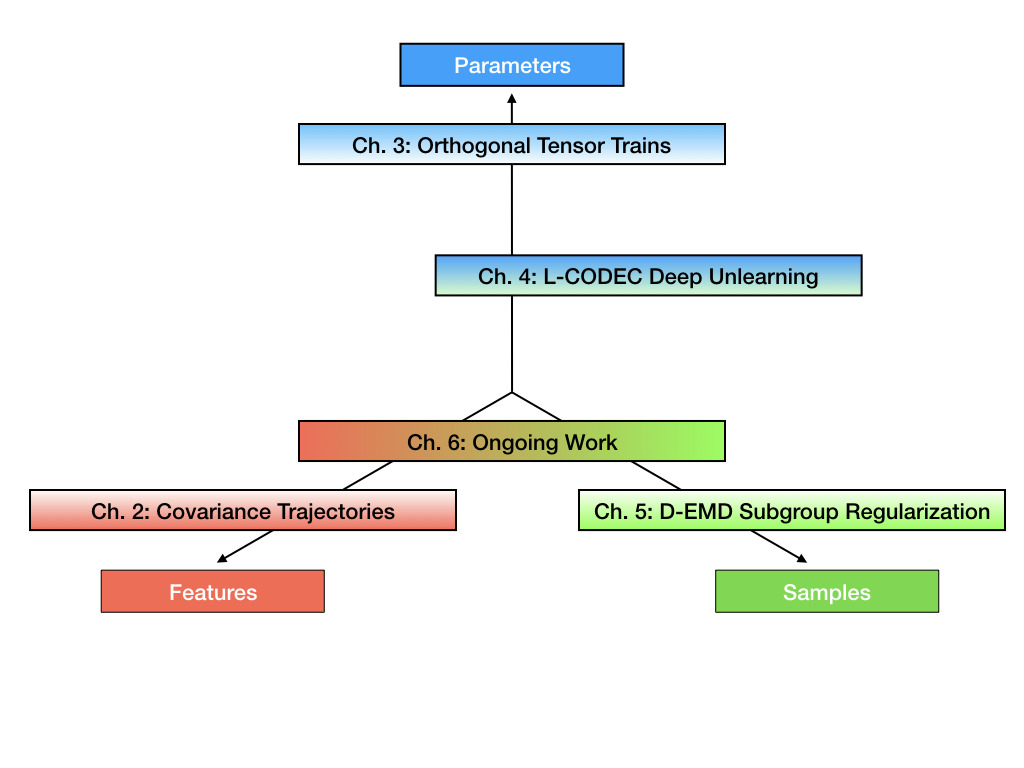
\includegraphics[width=0.95\linewidth]{diss/1_intro/figs/thesis_scope.png}
    \caption[Thesis Scope]{Thesis scope, projected over three representative axes. {\color{red} update chapter numbers shift by 1}}
    \label{fig:scope}
\end{figure}

\subsection{Second-Order Modeling and Group Difference Analysis over Time}

Recent results in coupled or temporal graphical models offer schemes for estimating the relationship structure 
between features when the data come from
related (but distinct) longitudinal sources. A novel application of these ideas is for analyzing group-level differences, i.e., in identifying if {\em trends} of estimated objects (e.g., 
covariance or precision matrices) are different across disparate conditions (e.g., gender or disease). Often, poor effect sizes make detecting the \textit{differential} signal 
over the {\em full} set of features difficult: for example, 
dependencies between only a {\em subset of features} may manifest differently across groups.
We first suggest
a parametric model 
for estimating trends in the space of $\SPD$ matrices as a function of one or more covariates.
We will then generalize scan statistics to graph structures, 
to search over distinct subsets of features (graph partitions) whose temporal dependency structure may show statistically 
significant group-wise differences.
We will theoretically analyze the Family Wise Error Rate (FWER) and bounds on Type 1 and Type 2 error. 
On a cohort of individuals with risk factors for Alzheimer's disease (but otherwise cognitively healthy), 
we 
find scientifically interesting 
group differences where the default analysis, 
i.e., models estimated on the full set of features, do not survive reasonable 
significance thresholds. 
% Preliminary work on this was published in \citep{covtraj}.


\subsection{Efficient Tensor Representations for Feasible Temporal Deep Learning}

Modern deep networks have proven to be very effective for analyzing real world images.
However, their application in medical imaging is still in its early stages,
primarily due to the large dimension of three-dimensional images, requiring enormous convolutional or fully connected layers --
if we treat an image (and not image patches) as a sample. 
These issues only compound when the focus moves towards longitudinal analysis
through recurrent structures, and when a point estimate of model parameters is insufficient 
in scientific applications where a reliability measure is necessary.
Using insights from differential geometry, 
we will adapt 
the tensor train decomposition to construct networks
with significantly fewer parameters,
allowing us to train powerful recurrent networks on whole brain image volumes. 
We analyze 
the \textit{orthogonal tensor train},
and demonstrate its ability to express a standard network layer both theoretically and empirically.
We 
demonstrate its ability to 
effectively reconstruct whole brain volumes
with faster convergence and stronger confidence intervals
compared to the standard tensor train decomposition. 
We provide code and show experiments on the ADNI dataset
using image sequences to regress on a cognition related outcome.
% Preliminary work on this was published in \citep{ott}.

\subsection{Practical Unlearning via Large-Scale Conditional Independence Testing}

%With AI systems extensively using personal %data for model training, 
Recent legislation has
led to interest in {\em machine unlearning}, i.e., removing specific training samples from a {\em predictive} model as if they never existed in the training dataset. 
Unlearning may also be required due to  corrupted/adversarial data or simply a user's updated privacy requirement.
For models which require no training ($k$-NN), 
simply deleting the closest original sample can be effective. 
%However, it is not clear how such approaches can be used to unlearn 
%models that contain rich information learned from the original data.
But this idea is inapplicable to models which learn richer 
representations.
%from data. 
%Recently, optimization-based unlearning estimators have been proposed, but 5their 
Recent ideas leveraging optimization-based updates
scale poorly with the model dimension $d$,  
due to 
inverting the Hessian of the loss function. %with an overall cost of $O(d^3)$ 
%is prohibitive.
We describe
a variant of a new conditional independence coefficient, 
L-CODEC, to identify a subset of the model parameters with the most semantic overlap on an individual sample level. 
Our approach completely avoids the need to invert a (possibly) huge matrix. 
By utilizing a Markov blanket selection, 
we find
that L-CODEC is also suitable for deep unlearning,
as well as other applications in vision.
Compared to alternatives, L-CODEC makes approximate unlearning possible 
in settings that would otherwise be infeasible, 
including vision models used for face recognition, 
person re-identification 
and NLP models that may require unlearning samples identified for exclusion.
% Preliminary work on this will appear in \citep{lcodec}.


\subsection{Reducing Subgroup Fairness via High Dimensional Earth Mover's Distances}

Optimal transport has recently emerged as a useful tool for machine learning through its connections with geometry, statistical machine learning, and through practical algorithms. Existing methods that leverage optimal transport often  regularize using  a Wasserstein metric or by computing barycenters, for example. %which are effective when distributions are continuous and known, or when measures of interest are discrete.
% Our formulation allows for a discretization of continuous measures that drop in directly to classical  formulations of the Earth Mover's Distance. 
We leverage optimal transport, except that we take advantage of a recently-introduced algorithm that computes a generalized earth mover's distance.
Not only is this algorithm computationally cheaper to compute compared to existing barycentric measures, but our method has the additional  advantage that gradients used for backpropagation can be directly read off of the forward pass computation, which leads to substantially faster model training.
We provide technical details about this new regularization term and its properties, 
and 
experimental demonstrations of improved training speed over existing Wasserstein-style methods.

{\color{red}
\subsection{Understanding Latent Spaces via Conditional Independences}

The final chapter of this thesis applies some of the tools developed above in the analysis of latent spaces in recent large scale models.
% In these studies, 
% we aim to identify conditionally independent features and subjects that are particularly important to the prediction and estimation of
% key disease outcomes,
% as a function of a number 
% of demographic, neuropsychological,
% genetic,
% and imaging data collected as 
% part of an ongoing consortium 
% to understand the progression
% of Alzheimer's disease in younger, 
% asymptomatic populations.
% In what follows we present
% exploratory analysis
% on a small, easily 
% digestible subset of the available data,
% that lays the foundation for
% further analysis.
}
% This work is the most forward looking, and aims to be a stepping stone toward a rigorous 

\section{Outline}
Chapter 2 covers the essential background necessary for the developments presented in the following chapters, including specifics of graphs and hypothesis testing, as well as relevant modern methods for learning and optimization.
In Chapters 3 through 7, we describe four perspectives to address subset identification.
Chapter 3 explores and focuses on the identification of feature subsets varying over time.
In Chapter 4 we describe a method of constraining the parameter space in a particular manner
that enables more efficient large scale neural networks.
Next, Chapter 5 provides a solution to the machine unlearning problem,
enabled through a particular conditional independence parameter selection scheme, vastly reducing network update costs.
Chapter 6 ends with a unique solution to subgroup fairness, 
where we take advantage of an efficient solution to
the $d$-dimensional earth mover's problem
to regularize large models when the number of subgroups can be large.
{\color{red} Chapter 7 describes future work, focused on applying a particular solution from Chapter 5 to understanding relationships among features in latent spaces learned by large generative models.}


%%%%%%%%%%%%% 
% Some old stuff

% Significant progress in the modern development of machine learning has
% been built upon connections and patterns identified across myriad
% interdisciplinary fields of study.
% Up through the mid 2000's, 
% many of these methods were inspired by and interested in 
% highly focused and constrained problems. 
% With a reasonably sized input domain, could a model of roughly equal size be used to
% predict some output?
% Linear regressors, decision trees, and support vector machines were all answers to these questions, with their own
% varying degrees of scaling and complexity.
% These methods necessitated carefully constructed formulations with specific restrictions to the learnable function class,
% enabling straightforward analysis 
% for provable performance guarantees 
% and easy identification of critical training samples and important input features.

% Contemporary machine learning, however, has a vastly different modus operandi. 
% Driven in large part by the exponential growth of available computation via Moore's Law, \textit{deep learning} has fallen squarely in the realm of \textbf{over-parameterized} models.
% With these overparametrizations and computation capacity, the typical learning questions posed as maximizing accuracy or reducing error have largely been addressed for even large scale problems.
% As such, complementary questions have led to subfields focusing on other performance measures, such as robustness, fairness, interpretability, and explainability.
% Many solutions to these questions end up looking back at answers found for the under- or non-parametrized settings.
% While nascent, these approaches 
% attempt to fill the gap between
% statistical and deep models to enable similar measures of sample influence, feature importance, and model analysis. 
% Most notable amongst these newer approaches is that of (Self)-Attention in Neural Networks \citep{sutskever2014sequence,vaswani2017attention}.
% Other proposals 
% end up looking back at the types of analysis typical of those more classical under-parametrized or nonparametrized methods.

% Not limited to previous developments in learning or computation theory, the arguably most valuable contributions toward the exponential reduction in model error can be attributed to influences and intuitions taken
% from biology, psychology, neuroscience, and even XXX \citep{srivastava, etc}.
% Perhaps one explanation as to why this phenomenon exists may be attributed to the way in which deep learning evolved. 
% The classical learning goal of function approximation lends itself nicely to a system which allows for arbitrary complexity via simple changes (e.g., addition of neural network layers). % Foundational works building on the original neural networks particularly have taken advantage of constraining this space of functions to search over: 
% the most seminal case being those of convolutional filters for imaging data. 
% While ``constraints" of this form have helped tremendously in model performance on modern vision and language machine learning tasks (GANs, Recurrent Networks, Residual Layers, Transformers, etc.), the ability to identify \textit{subsets} of important samples, input features, and model parameters has lagged significantly behind the development of these methods.
% Recently larger interest has been taken by the community to understand and interpret models with this view, only after extremely large and opaque models have become ubiquitous.
%This lag directly explains the more recent interest in developing methods for understanding and interpreting large scale machine learning models. % OTT
\chapter{Introduction} \label{chap:intro} 

Modern applications of machine learning in a broad range of industrial and consumer-facing systems have become ubiquitous.
Most interactions with daily technologies now intrinsically involve 
a request to some ``smart`` system in the ``cloud'', 
where those interactions range from
a request for map directions 
to simply loading a webpage.
Neural network models, and the recent advances of deep learning,
have enabled these systems that 
make such applications possible.
These models have achieved
human-level performance on learning tasks
including image classification~\citep{resnet,alexnet}, image segmentation~\citep{segmentation}, video analysis~\citep{zhang2016video}, text understanding and generation~\citep{bert,gpt}, and have slowly begun to solve more fundamental scientific problems such as protein folding~\citep{protein} drug discovery~\citep{drugdisc}, and medical diagnosis~\citep{diag}.
While this performance is largely attributed to model size,
the abundance of high quality training data
has equally contributed to real world performance,
enabling model training over millions of real world samples~\citep{imagenet,laion},
and potentially billions of synthetic samples via environment simulation~\citep{mcts}.

While deployment in some domains (recommender systems, object detection) may benefit almost unconditionally from this vastly expanded capability, rightful hesitancy has limited their widespread use in particular applications where impacts on individuals, people, or environments may be at stake.
These ``last mile'' concerns take a few forms.
% Because a completely accurate model is still out of reach, an important question that needs to be answered is: which inputs or individuals are being given incorrect outcomes, and why?
% maybe a sentence suggesting unlearning/removal
In mission critical applications such as medical diagnosis, 
the impact of an error can be extremely large,
even if a misprediction happens extremely infrequently.
Additionally, large scale model training and architecture search
can require exorbitant amounts of energy producing high emissions,
and their scale can limit market participants
to only large actors with vast existing resources.
The accessibility and effectiveness of these models can also vary significantly based on the training data, and disparate outcomes can be exacerbated by existing social inequity.

While existing human or ``natural'' systems that these models aim to assist are not perfect, 
our real world has developed norms and regulations that 
enable them to function.
A medical diagnosis might require a physician to explain what symptoms led them to that particular conclusion.
Energy metering and carbon taxes may be applied to limit
emissions.
Regulatory satisfaction may require 
analysis proving equal opportunity,
or that specific protected classes
are not used in decision making.
% Specifically, these can include ideas as simple as the Hippocratic Oath and medical malpractice insurance, to asking your doctor what symptoms lead them to a particular diagnosis.
These ideas are difficult to directly translate to automated machine learning systems,
but proxies have been identified that we can build upon.

These norms and regulations answer a number of questions we may also try to pose to our machine learning models.
What is the cost to learn this task?
What led to this particular outcome?
Why is this outcome different from another?
% We will explore how these questions can be formulated concretely. 

If the answer to these questions is negative or unknown,  follow-up questions all take an interesting form:
Can we learn a smaller model with similar performance? 
Can we identify the most important features? 
Which individuals or groups are being treated unfairly, and can we change that?
These questions ask us to identify a \textit{subset} of some relevant set, dependent on setting, and this identification is our focus here.

% Moving specifically to machine learning methods,
Taking a step back, let's take a look at a representative system. Figure~\ref{fig:dl} illustrates a typical learning pipeline. 
A dataset is collected and used to train a model, by minimizing the error over
those samples in the dataset (top).
A ``sample'' can be a single measured value, or it can
be a large, highly structured object with many ``features.''
The model is made up of some ``parameters'' that are 
tuned during training to learn a good predictor over the training dataset.
This model is then used to predict, or \textit{infer}, on new
data seen ``in the wild'' (bottom).
Our questions above are formally asking to identify \textit{subsets of these objects}: is a subset of the model parameters sufficient for learning? Which subset of the features are important for a prediction? Which subset of the dataset exhibit a specific attribute?
\begin{figure}
    \centering
    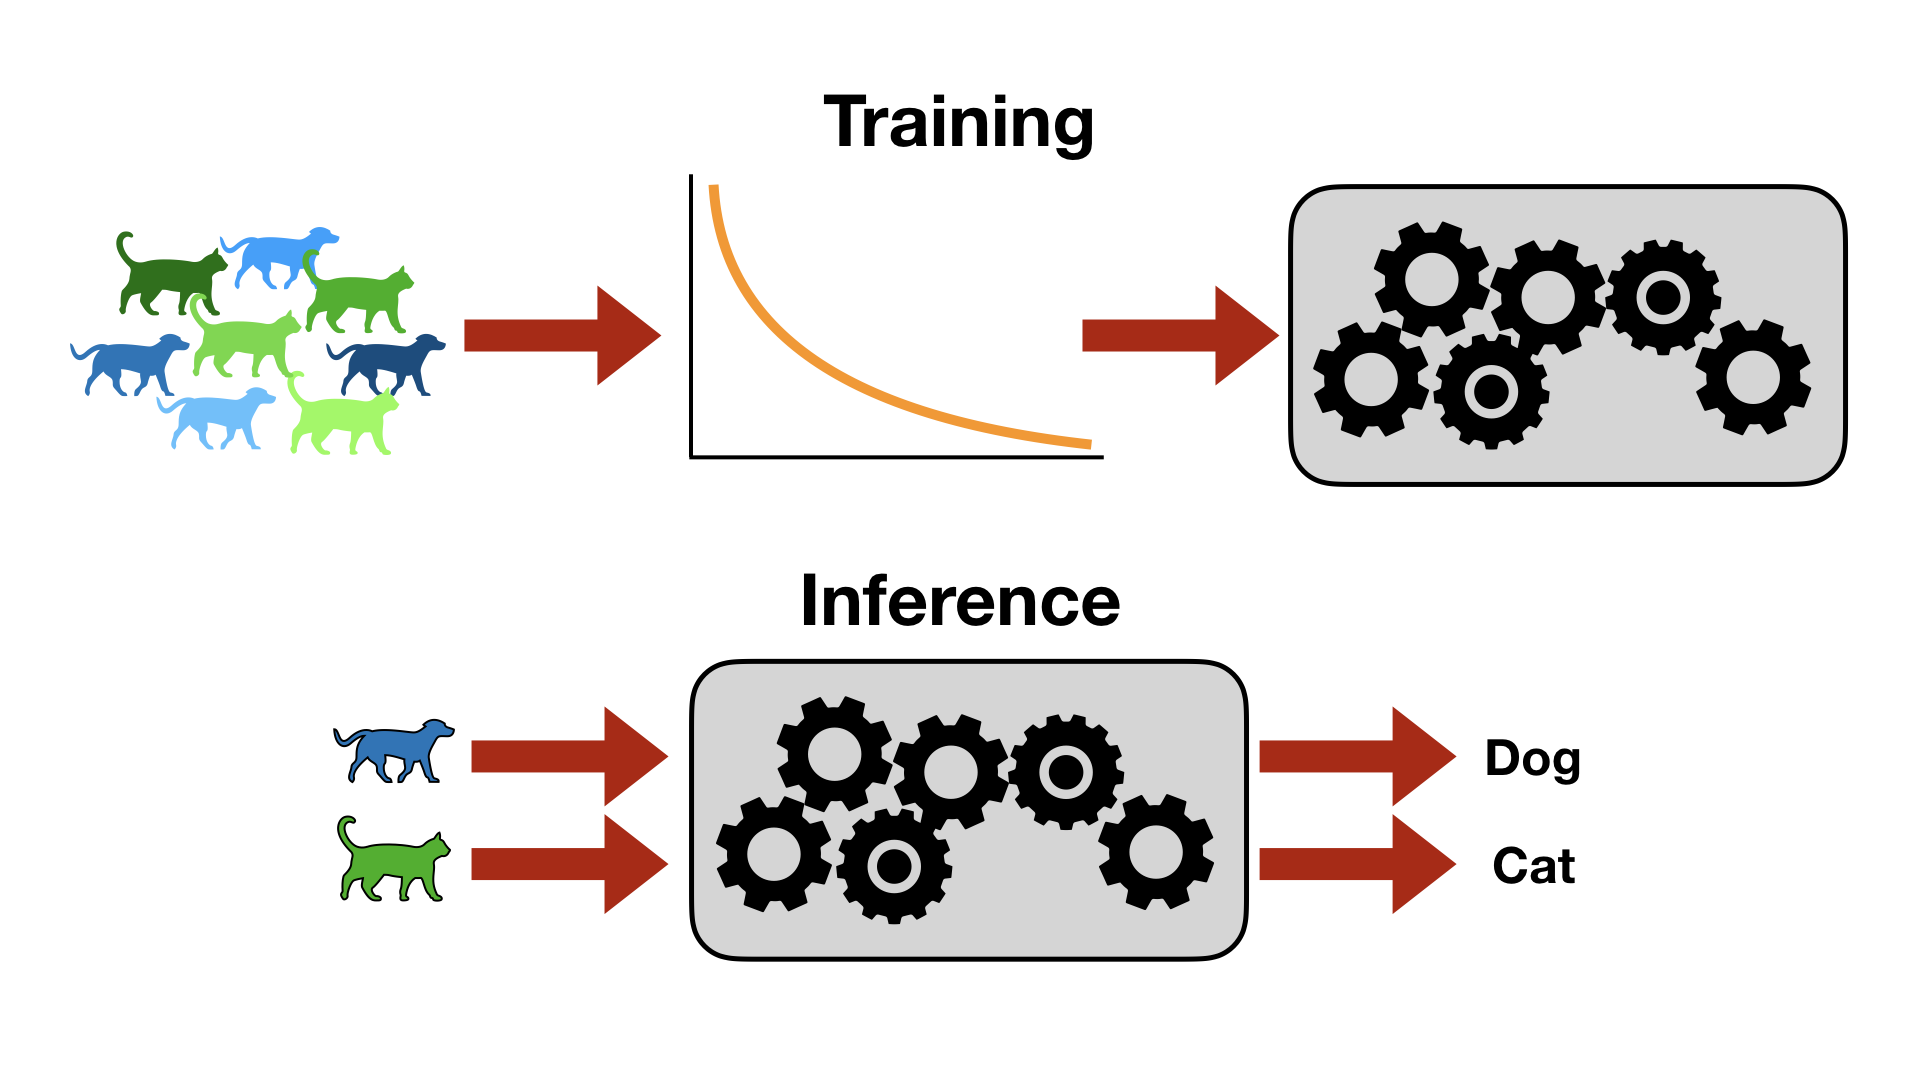
\includegraphics[trim={0 3cm 0 3cm},clip,width=0.95\textwidth]{diss/1_intro/figs/dl.png}
    \caption[Modern machine learning pipelines]{Machine learning training and inference visualization.}
    \label{fig:dl}
\end{figure}

% \textit{Explainability} can be seen as identifying important features of the input, as well as parts of the model (parameters) that ``light up`` for that input. \textit{Fairness} can be evaluated via measures over subsets of the data that correspond to specific groups. 

\begin{mdframed}[style=MyFrame]
\em 
\textbf{This thesis} focuses its main efforts on identifying these important subsets of model, feature, and sample space, to enable answering questions necessary for mainstream adoption of machine learning methods.
\end{mdframed}

% In this dissertation, we explore the sizes of these models, samples, and datasets, and 
% analyze under what situations 
% a smaller \textit{subset} of them may be sufficient or important
% for questions that run parallel to standard performance and accuracy measures.

Let us step a bit deeper into a basic illustrative example. In order to ease understanding, we can first begin with a basic formulation of learning methods, from which the questions above can take specific forms. 
Learning methods typically  try to identify a function mapping (model) that is able to complete a specific task at some high level of profficiency.
% In Figure~\ref{fig:dl}, a model is trained using examples of classification task (top), in order to accurately predict the class of a newly provided input (bottom).
% \begin{figure}
%     \centering
%     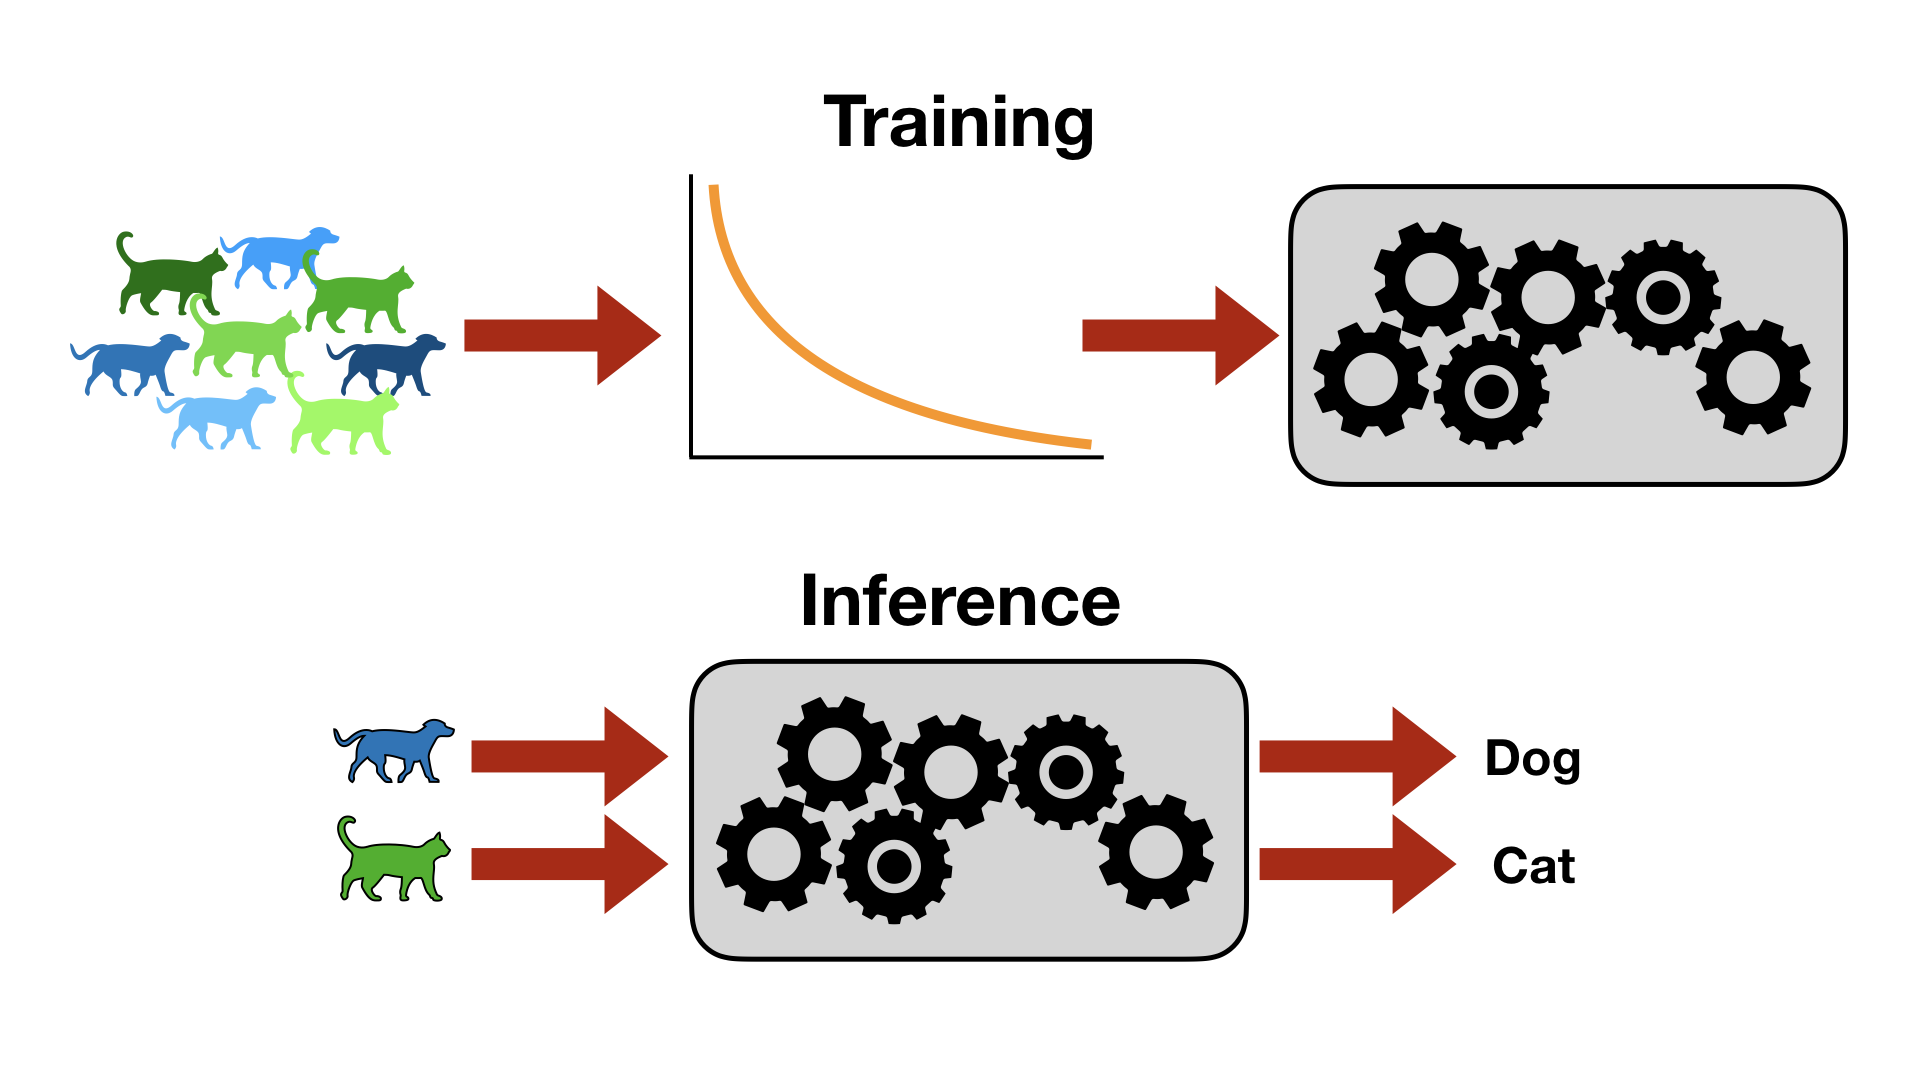
\includegraphics[trim={0 3cm 0 3cm},clip,width=0.95\textwidth]{diss/1_intro/figs/dl.png}
%     \caption[Modern machine learning pipelines]{Machine learning training and inference visualization.}
%     \label{fig:dl}
% \end{figure}
Say we have some dataset comprising of sample pairs $(x,y)$, where we wish to predict $y$ from $x$.
Our prediction, say $\hat{y}$, might be the output of some unknown function $f$ that we attempt to learn from training data. 
Let our approximation to this function be $\hat{y}:=\hat{f}(x)$.
This can take many forms, 
based on assumptions and prior information we may have on the relationships among the data. 
Consider the simple \textit{linear} case,
where we want to learn some parameter $w$ such that $y = w\cdot x$. 
Given $n$ sample pairs $(x_i,y_i)$ indexed by $i$, traditional statistics and optimization literature yield the following \textit{least squares} problem formulation, where we want to minimize the ``squared error'' between the observed values $y_i$ and the predicted $\hat{y}_i:= w\cdot x_i$:
\begin{align}\label{eq:lq}
\hat{f}:=\hat{w} = \mathop{\arg\min}_{w} \sum_{i=1}^n (y_i - w\cdot x_i)^2
\end{align}
This formulation expands without much change to a multi-dimensional form of the input $x$ and respectively, $w$: the canonical case where a number of features, or \textit{covariates} (e.g., symptoms), are used together to predict the outcome (e.g., diagnosis). 
If we are interested in which features of $x$ are important, we can look at the relative values of the learned ``weights'' $w$. In this simple setting, the importance of a feature (say $x^j$) can be exactly determined by the importance of the parameter ($w^j$).
A weight value far from zero may indicate that corresponding feature is important for diagnosis.
% If instead we are interested in which samples are most important, we can use existing methods for sample reweighting or methods that use standard assumptions to efficiently identify important subsets.

In this case and others, traditional statistical learning methods 
have been studied 
for many decades.
Linear regressors, decision trees, and support vector machines
have all been analyzed under these lenses.
% ,
% and as the modern machine learning community
% has returned to these questions recently,
% so has a renewed interest in their methods of analysis.
New research focuses
particularly on the differences
associated with moving from classical \textit{under-parametrized} models to
modern (deep) \textbf{over-parameterized} models: where
the model size vastly outnumbers the number
of input samples.
% , and may even be comparable to 
% the \textit{entire sample space.}
Methods for estimating the number of samples needed,
the time to learn a particular task,
and the generalization ability 
all require new perspectives in this regime.
While nascent, this research
attempts to fill the gap between
statistical and deep models to enable similar measures of sample influence, feature importance, and model understanding. 

\paragraph{A full picture.}
Let us expand our notation from the example above to consider this more general framing.
Consider a dataset $X:=\{x_i\}_{i=1}^n$ of size $n$ where each data point $x_i$ in the set $X$ is drawn from some underlying distribution over the domain $x_i \sim \cX^d$, 
with domain dimensionality (number of features) $d$.
A model $f$ is fit using a parametrization $\theta \in \Theta$,
with $\Theta$ the space of possible parametrizations (models) with some intrinsic dimension $p$. 
%While all three of these problems are closely related, they require different approaches. 
Generalizing the least squares``error measure'' from Eq.~\eqref{eq:lq} to an arbitrary \textit{loss} $\ell$, we have
\begin{align}\label{eq:learning}
    \hat{f}:=\hat{\theta} = \mathop{\arg\min}_{\theta\in\Theta} \sum_{x \in X} \ell(f_\theta(x_i))
\end{align}
From an analysis perspective, 
we might be interested in any one of 
(a) subsets of input features $\cC \subseteq \cX$ that are important for the downstream task,
(b) associating model subsets $\cP \subseteq \Theta$ with specific inputs or groups of inputs, or 
(c) subsets or subgroups of samples $S \subseteq \{X\}$ that are sufficient or representative of the entire dataset.

Crucially, an uninformed search for a subset is computationally infeasible. For a superset of size $n=|X|$, The set of all subsets is the power set, with a size of $2^{n}$! If an identification procedure requires looking over all of these and choosing a ``best'' one by some metric, the procedure will be limited to very small supersets.
Efficient methods have been developed in each of the three contexts above to avoid this exponential search.

\begin{figure}
    \centering
    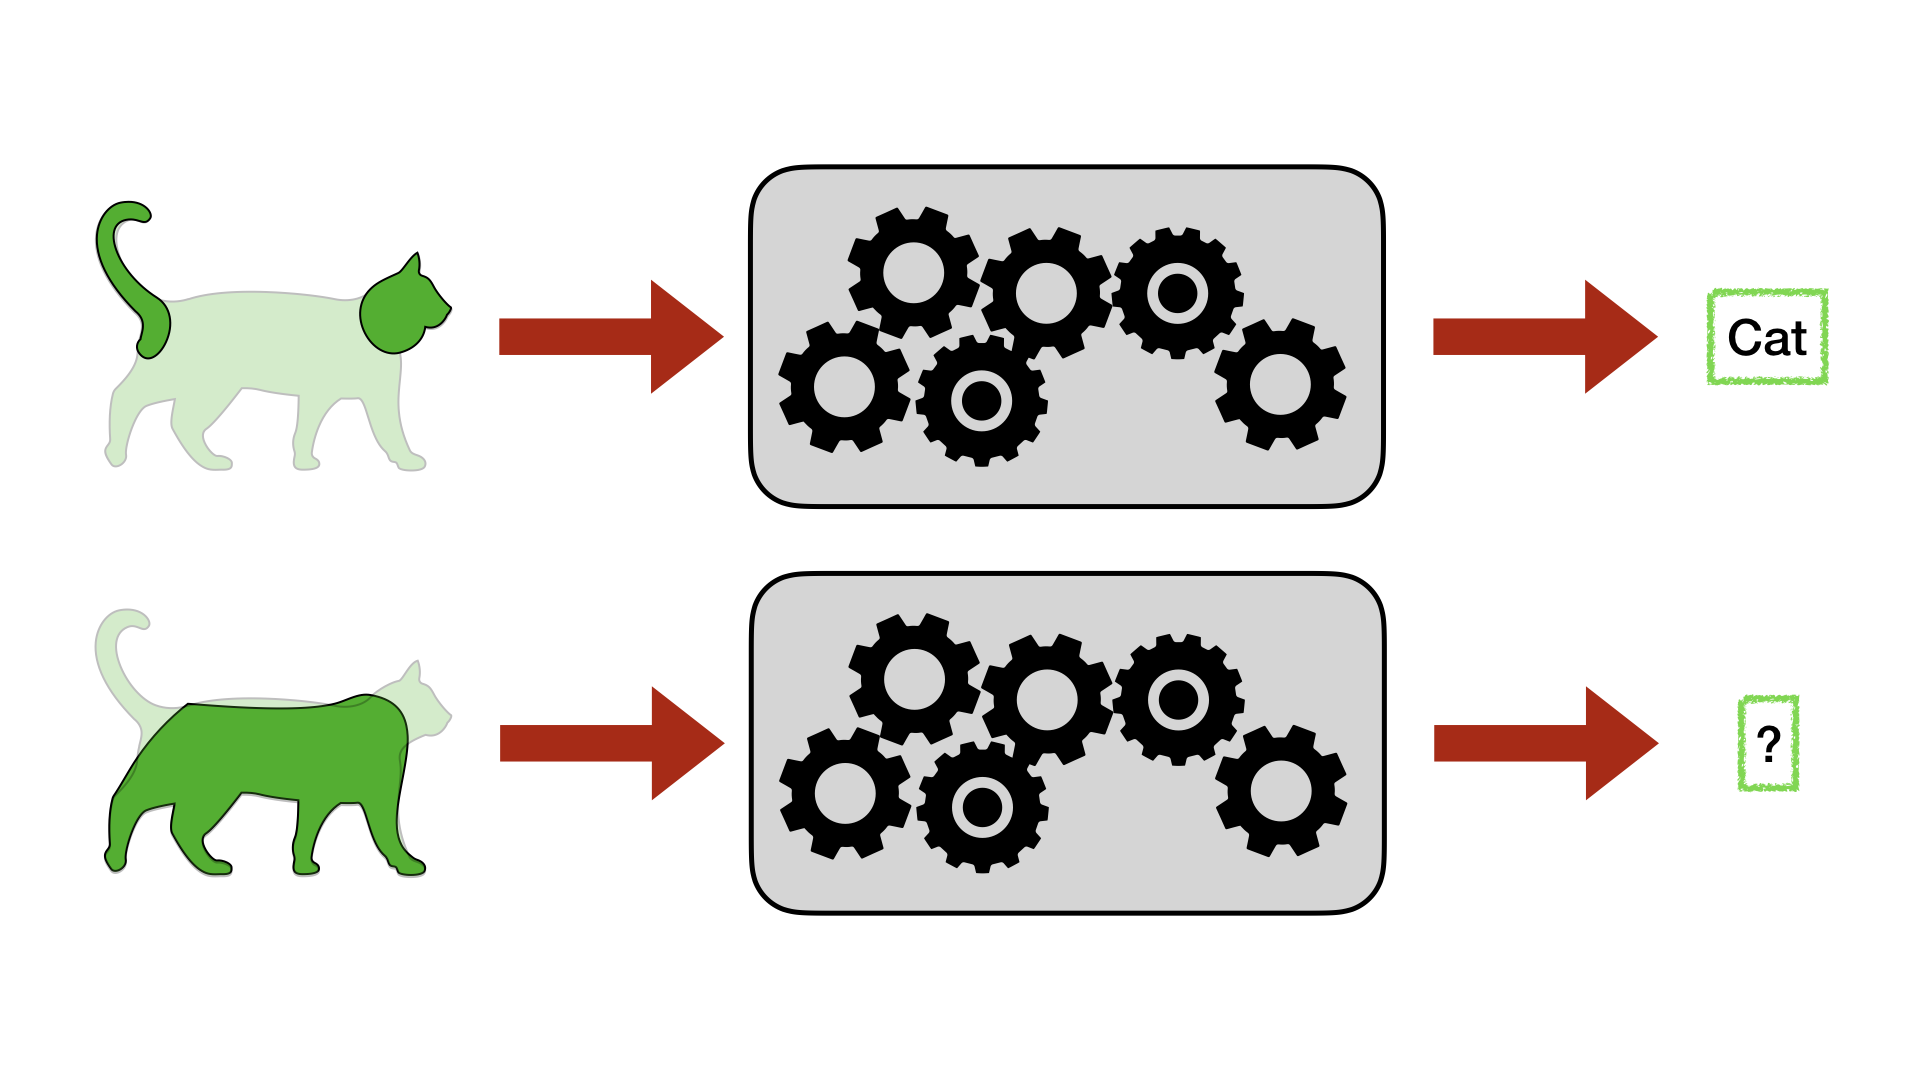
\includegraphics[trim={0 3cm 0 3cm},clip,width=0.9\textwidth]{diss/1_intro/figs/feat_select.png}
    \caption[Visualization of feature selection]{An example of identifying specific features important to the learning task.}
    \label{fig:feat_select}
\end{figure}
\paragraph{Feature Selection.} 
With more complex models $f$ compared to the linear case above, newer ``black-box'' methods have been developed for identifying important features. From the more pure statistics side, scan statistics~\citep{scanstat,scanstatlrt} allow for a structured ``scanning'' over the input space, skipping subsets unlikely to provide additional information for the measure of interest.
Further on the deep learning side, adaptations of sensitivity analysis, via noise addition and perturbations have found success~\citep{yeung2010sensitivity,zhang2015sensitivity}, alongside activation mapping~\citep{cam,selvaraju2017grad}.
These methods typically generate an analagous ``weighting'' over the input space, identifying features most salient for the specific task (Figure~\ref{fig:feat_select}).

\begin{figure}
    \centering
    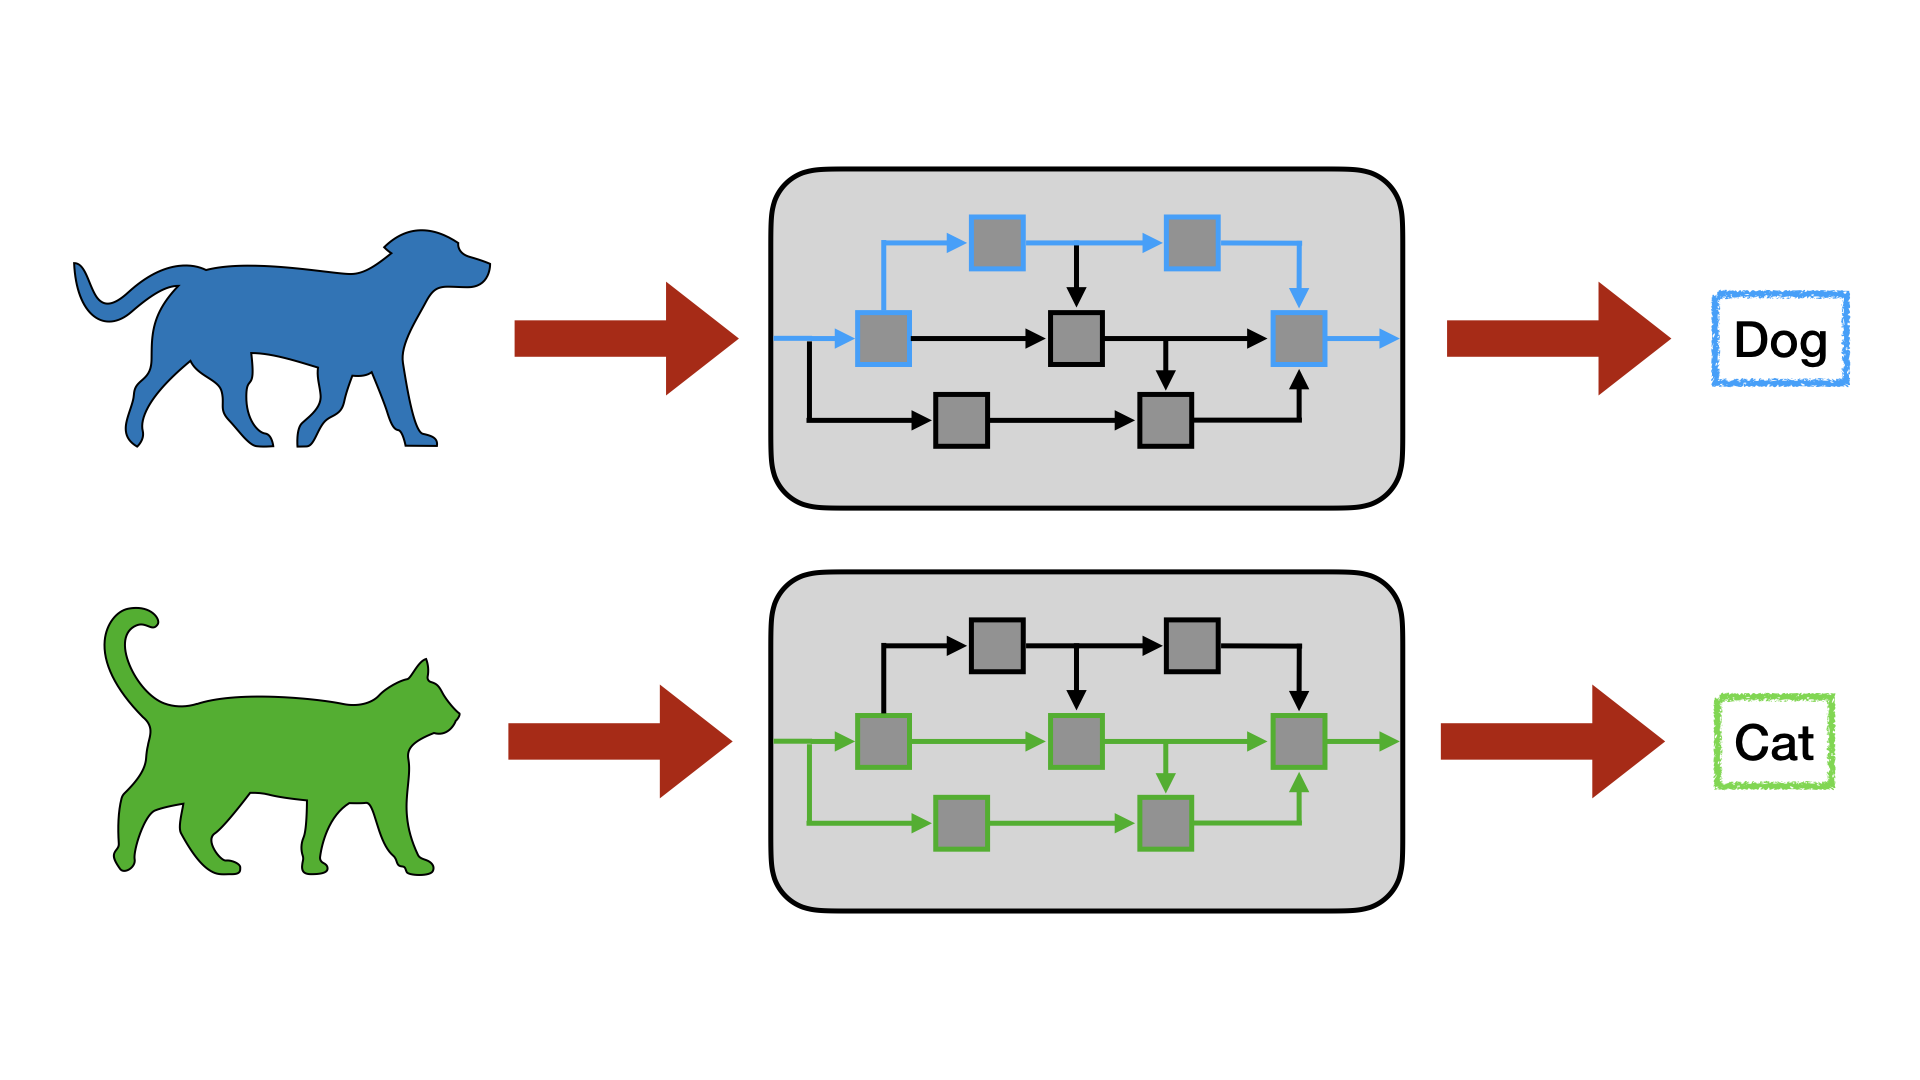
\includegraphics[trim={0 3cm 0 3cm},clip,width=0.9\textwidth]{diss/1_intro/figs/param_select.png}
    \caption[Visualization of parameter selection]{An example of identifying specific parameters important to the learning task.}
    \label{fig:param_select}
\end{figure}
\paragraph{Parameter Selection.} 
Selection in the model space generally takes two forms. First, as a prior, restriction, or assumption over the model space, and second, as a post-hoc method for an ``explainable'' proxy.
Regularization, sparsity, and gating methods are often used independent of the type or size of the model, to encourage the solution to fall within a specific region of the model space.
% In non-deep settings these methods come with strong theoretical guarantees. 
The theoretical underpinnings of these methods in deep learning are still being actively researched~\citep{hardt2016train,jacot2018neural,neyshabur2014search}, but the methods have nonetheless been effective in practice. 
On the post-hoc side, of particular interest are the parameters relevant to specific regions of the input space \textit{after} training (Figure~\ref{fig:param_select}). Here, recent analysis of deployed networks has shown this to be true~\citep{bau2017network,fong2018net2vec}, and current work continues to explore these network regions to aid in interpretability and explainability.

\paragraph{Sample Selection.} Many methods have been developed for outlier detection within training or testing sets~\citep{huang2020feature,ren2019likelihood} \textit{after} training, as well as methods for understanding sample influence~\citep{koh2017understanding,golatkar2020eternal,huang2020feature} . ``In-the-loop'' methods for accounting for ``outlierness'' behave similarly to accounting for group or individual fairness while training~\cite{mehrabi2021survey}. Unfortunately, once samples are identified in some manner, post-hoc adjustments to a trained model are generally very difficult. Recent work has focused on ``unlearning'', or removing a sample's influence on a model without retraining. If specific samples can be uniquely identified, performance and privacy reasons may require these specific interventions to reduce the ``influence'' of that sample subset.
\begin{figure}
    \centering
    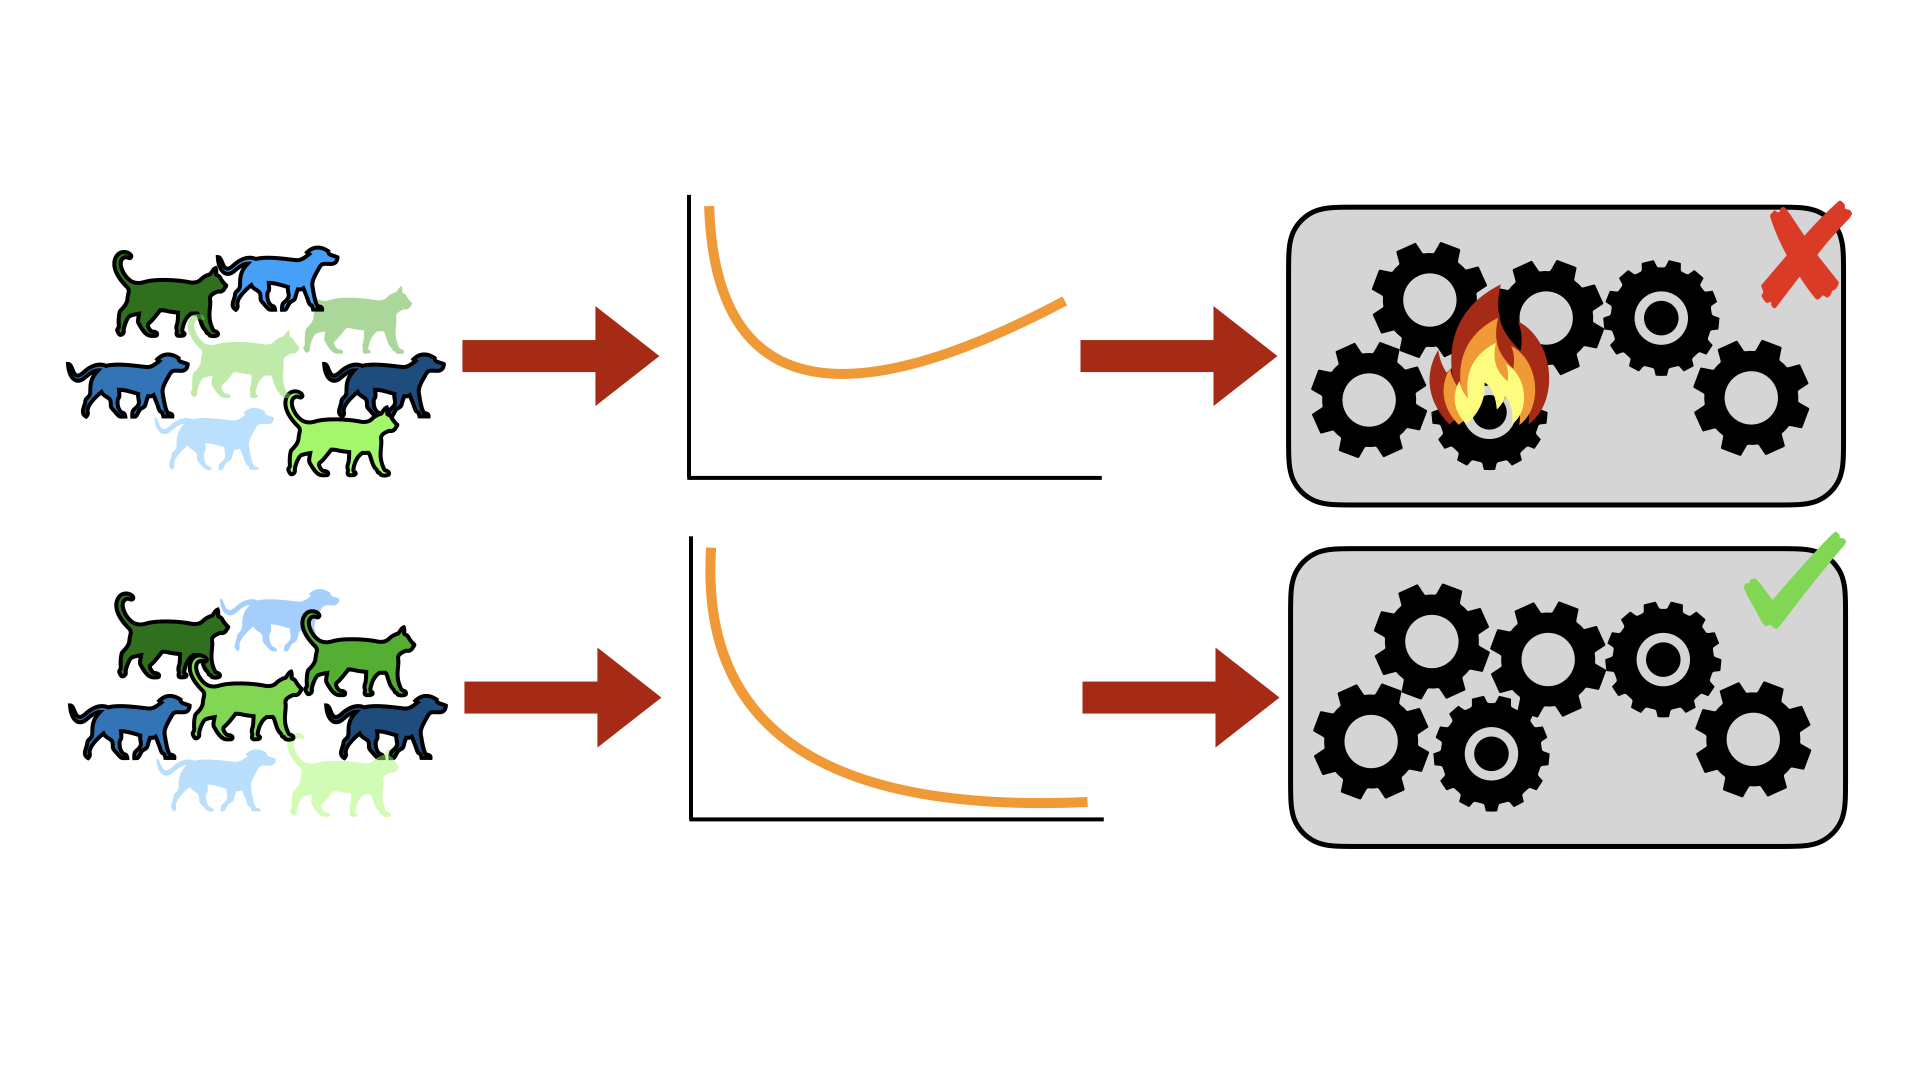
\includegraphics[trim={0 4.5cm 0 4cm},clip,width=0.9\textwidth]{diss/1_intro/figs/sample_select.png}
    \caption[Visualization of sample selection]{An example of identifying specific samples important to the learning task.}
    \label{fig:sample_select}
\end{figure}


\begin{mdframed}[style=MyFrame]
\textbf{ Thesis Goal: }
\em Identify, construct, and evaluate methods for \textbf{efficient} subset identification in modern machine learning feature, model, and input spaces.
\end{mdframed}

\section{A Few Motivating Examples}
Consider a traditional machine learning classification task in which we would like to predict whether an individual has a specific disease condition based on a medical resonance image (MRI) scan of their brain. Our input feature $x$ may consist of a 3D-array of values in $\RR^{\cI\times \cJ\times \cK}$ measuring some intensity of the imaging modality at each voxel, indexed by a tuple $(i,j,k) \in (\cI,\cJ,\cK)$.
Our outcome variable $y$ may simply be a binary label of whether the input scan has been labeled by a radiologist as one demonstrating typical disease characteristics.
Using an off the shelf 3D convolutional neural network with adjustments to match our input size, we can very quickly set up and train a system to predict disease presence with a high degree of accuracy.

\paragraph{Example 1.}
With a prediction for a specific scan, or predictions over a number of scans, we might be interested in identifying which regions of the brain are most important for diagnosis. These regions, $R \subset \cR:=\RR^{x\times y\times z}$, can be specific groups of pixels in the image that may correspond to known functional networks. Methods such as attention and class activation maps may work here, but there are a few issues. The number of samples available to learn a model is very small compared to the both the dimension of the input and the number of parameters in the model, i.e., $n \ll p$ and $n \ll d$. Thus it is very easy to overfit, and for areas of interest to be associated with intricacies of particular input data rather than true, real differences defined by the disease.

Furthermore, recent medical imaging studies have moved past simple difference detection: trends over time, and the ability to predict {\em future} disease development have by far become the setting of most interest.
Given an image of a healthy individual, is it possible to predict what their scan, or their future disease diagnosis, may be up to 10, 20, or more years in the future?
If a number of scans have been collected over some timeframe, can the \textit{trajectory} of the individuals' development be extrapolated to estimate progression?
As traditional models extended for temporal analysis grow in both size and complexity,
a number of subproblems explicitly related to model and input subspaces arise. In this thesis we address two such problems: \textbf{statistically rigorous identification of temporally evolving subsets}, and \textbf{characterizations of deep models that enable efficient training of recurrent models with large scale time-varying data}.
    
\paragraph{Example 2.}
With the rapid growth of AI and machine learning applications has come valid concerns regarding both guarantees of privacy.
Recent technology legislation has made the importance clear in all aspects of data use,
and particular projects and groups have demonstrated that machine learning is not independent of
this need \citep{Exposing}.
A new issue raised within this intersection is the ``right to be forgotten".
If a model has been trained with a particular users' data, 
they should have some recourse or right
to both remove their data from the training set,
and also know that the model has not learned from their data.
On the surface, this poses a significant problem for model builders
and organizations that spend large amounts
of time and resources in 
training deep learning models.

In the medical imaging example above this is especially important: with fewer samples it is more likely that information about any particular one could ``leak'', and the model's performance may degrade significantly as a relatively large percentage of it's training data is removed.
Thus tailored methods must be developed to ensure both privacy and performance, without requiring full retraining.
As we will see, 
\textbf{identification of model parameter subsets}
that are particularly important
for a particular sample's influence
in a model enables \textit{efficient machine unlearning}.

\paragraph{Example 3.}
From an alternative perspective, we may want to identify specific samples rather than have them specified a priori.
Traditionally a rigorous area of study under classical statistics, outlier detection and accounting have become a subfocus for many within the machine learning community as well \citep{golatkar2020eternal,golatkar2020forgetting,huang2020feature,ren2019likelihood}.
While subgroups of input samples may be outliers, it is more often the case that they represent known heterogeneity within the data. 
These differences may be marked using 
group information known a priori, and 
most learning tasks aim to learn tasks
in a \textit{subgroup-independent} manner.
In our disease prediction model above,
these groups could simply be stratified by the type of scanner used to acquire the image, but it could also
be a systematic difference correlated with some protected attribute. {\color{red} sentence about original brain atlas for registration being eurocentric}
This can directly lead to disparate performance and results on \textit{all} individuals outside of that group.
Optimization and regularization methods with this focus come under the umbrella of model fairness.
However, many existing methods do not scale well to larger models or as the number of subgroups grows, as is often the case when intersections of protected classes must be considered. Here we identify and construct a particular solution for \textbf{groupwise fairness that enables efficient in the loop fairness regularization}.

% What features are most important for prediction?
% Which samples were most important for my training?
% Can we understand when a model is certain or uncertain about its output?
% Are there layers in my network that have learned a particular subtask?
% Questions of robustness, bias, influence, fairness, and importance have become central questions to contemporary machine learning research \citep{doshi2017towards,mehrabi2021survey,amodei2016concrete}.
% machine learning, etc.

% Feature selection in the case of
% typical regression or classification 
% takes some form of learning parameters $\theta$ that allow for $\hat{y} = f_\theta(x)$ to be close to the true outcome of interest $y$.
% While forms of data $X := (x,y)$ may simply be continuous and real-valued, modern machine learning has greatly expanded formulations of the classical learning problem to include a wide variety of structured learning problems~\citep{nowozin2011structured}. 
% Consider the case when a high-dimensional input is used to predict an output with a highly-parametrized model. 
% Once learned, obvious questions arise as discussed above: are there specific low-dimensional spaces in either the input or the model space that are most important or necessary for the global learning problem of interest? Are there specific subspaces associated with particular subproblems of the global problem?
% The machine learning literature has come up with a number of ways to identify analogs of these spaces, 
% including extensions of sensitivity analysis to deep learning~\citep{yeung2010sensitivity,zhang2015sensitivity}, and constructing and identifying nonzero model subsets via particular model choices such as activations~\citep{selvaraju2017grad} and regularizers.
% In classical settings these are well understood: decision trees naturally provide ease of interpretibility via the information used to choose splits, and both linear and kernel support vector machines have been analyzed to provide for measures of sample importance via distances to the margin as well as feature importance via weights defining the learned hyperplane~\citep{Mitchell97}.
% Attention and saliency maps have emerged as popular new methods,
% given their ease of implementation and interpretation~\citep{sutskever2014sequence,vaswani2017attention,selvaraju2017grad}.
% By learning dimensions of a given input that are particularly important, either in a hard (binary) or soft (continuous weighting) manner, model builders are better able to understand and interpret what a model has learnt.
% The specific ideas of attention notwithstanding, many of these existing methods are far removed from traditional hypothesis testing frameworks.
% While some work has begun in this direction~\citep{tansey2018black},
% there remains a gap in direct identification of subsets and structures in these spaces that can be defined in statistically rigorous manners.

% \begin{figure}
%     \centering
%     \includegraphics[width=0.5\textwidth]{example-image-a}
%     \caption[A simple subset selection example]{\color{red} Identifying and selecting in MRIs, subset, sample, model ID.}
% \end{figure}

% \paragraph{A specific example.} 

% ------------------------------------------

% below here will be moved and arranged with the "selection" sections and here if relevant

% ------------------------------------------

% While attention can be directly applied to the network in order to identify ``hotspots" in the input space relating to the learned classification task, 
% given the high-dimensional nature of the input
% and the relatively small sample size 
% associated with medical imaging data, 
% it is very likely that an area of interest identified
% may be an intricacy of the training samples used rather than truly a region of disease signal.
% Class activation maps (CAMs) may be unclear, and can often associate with image artifacts unrelated to the scientific task~\citep{adebayo2018sanity}.
% Methods of generalization may help to increase confidence in identified regions, but statistical guarantees often remain out of reach.

% Furthermore, most recent problems associated with medical data have moved past simple difference detection: trends over time, and the ability to predict {\em future} disease development has by far become the setting of most interest.
% Given an image of a healthy individual, is it possible to predict what their scan, or their future disease diagnosis, may be up to 10, 20, or more years in the future?
% If a number of scans have been collected over some timeframe, can the \textit{trajectory} of the individuals' development be extrapolated to estimate progression?
% As traditional models extended for temporal analysis grow in both size and complexity,
% a number of subproblems explicitly related to model and input subspaces arise. Here we address two such problems: \textbf{statistically rigorous identification of temporally evolving subsets}, and \textbf{characterizations of deep models that enable efficient training of recurrent models with large scale time-varying data}.

% A sample's particular influence on model parameters aside, the identification of influential samples or subsets of samples more generally is of independent interest. 
% Traditionally a rigorous area of study under classical statistics, outlier detection and accounting have become a subfocus for many within the machine learning community as well \citep{golatkar2020eternal,golatkar2020forgetting,huang2020feature,ren2019likelihood}.
% While subgroups of input samples may be outliers, it is more often the case that they represent known heterogeneity within the data. 
% These differences are typically marked using 
% group information known a priori, and 
% most learning tasks aim to learn tasks
% in a \textit{subgroup-independent} manner.
% Optimization and regularization methods with this focus come under the umbrella of model fairness, and instead of identifying and boosting independences within the model or data, we aim to minimize them.
% However, many existing methods do not scale well as the number of subgroups grows, as is often the case when intersections of protected classes must be considered. In the sequel we identify and construct a particular solution for \textbf{groupwise fairness that enables efficient in the loop fairness regularization}.

\begin{mdframed}[style=MyFrame]
\em 
Here we focus our effort on identifying these important subsets of model, feature, and sample space for feature association, model size reduction, model unlearning, and, fairness. Specifically, taking advantage of both existing statistical and geometric methods, we develop new methods for localizing subsets in a range of settings from hypothesis testing to deep learning.
\end{mdframed}

\section{Thesis Scope and Contributions}

We explore the intersections of classical statistical and geometric constructions with modern machine learning methods. 
Figure~\ref{fig:scope} shows the overall scope projected along three axes: feature, parameter, and sample spaces.
Below we briefly introduce the main problems studied in this thesis.
\begin{figure}[!ht]
    \centering
    % \includegraphics[width=0.99\linewidth]{scope.pdf}
    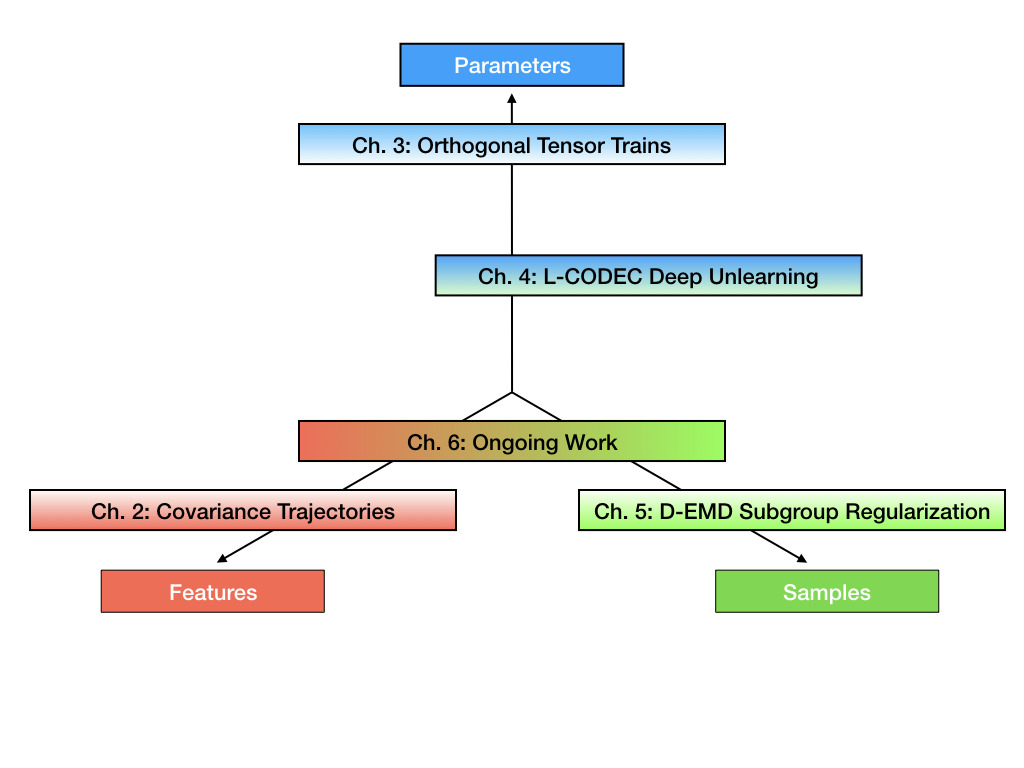
\includegraphics[width=0.95\linewidth]{diss/1_intro/figs/thesis_scope.png}
    \caption[Thesis Scope]{Thesis scope, projected over three representative axes. {\color{red} update chapter numbers shift by 1}}
    \label{fig:scope}
\end{figure}

\subsection{Second-Order Modeling and Group Difference Analysis over Time}

Recent results in coupled or temporal graphical models offer schemes for estimating the relationship structure 
between features when the data come from
related (but distinct) longitudinal sources. A novel application of these ideas is for analyzing group-level differences, i.e., in identifying if {\em trends} of estimated objects (e.g., 
covariance or precision matrices) are different across disparate conditions (e.g., gender or disease). Often, poor effect sizes make detecting the \textit{differential} signal 
over the {\em full} set of features difficult: for example, 
dependencies between only a {\em subset of features} may manifest differently across groups.
We first suggest
a parametric model 
for estimating trends in the space of $\SPD$ matrices as a function of one or more covariates.
We will then generalize scan statistics to graph structures, 
to search over distinct subsets of features (graph partitions) whose temporal dependency structure may show statistically 
significant group-wise differences.
We will theoretically analyze the Family Wise Error Rate (FWER) and bounds on Type 1 and Type 2 error. 
On a cohort of individuals with risk factors for Alzheimer's disease (but otherwise cognitively healthy), 
we 
find scientifically interesting 
group differences where the default analysis, 
i.e., models estimated on the full set of features, do not survive reasonable 
significance thresholds. 
% Preliminary work on this was published in \citep{covtraj}.


\subsection{Efficient Tensor Representations for Feasible Temporal Deep Learning}

Modern deep networks have proven to be very effective for analyzing real world images.
However, their application in medical imaging is still in its early stages,
primarily due to the large dimension of three-dimensional images, requiring enormous convolutional or fully connected layers --
if we treat an image (and not image patches) as a sample. 
These issues only compound when the focus moves towards longitudinal analysis
through recurrent structures, and when a point estimate of model parameters is insufficient 
in scientific applications where a reliability measure is necessary.
Using insights from differential geometry, 
we will adapt 
the tensor train decomposition to construct networks
with significantly fewer parameters,
allowing us to train powerful recurrent networks on whole brain image volumes. 
We analyze 
the \textit{orthogonal tensor train},
and demonstrate its ability to express a standard network layer both theoretically and empirically.
We 
demonstrate its ability to 
effectively reconstruct whole brain volumes
with faster convergence and stronger confidence intervals
compared to the standard tensor train decomposition. 
We provide code and show experiments on the ADNI dataset
using image sequences to regress on a cognition related outcome.
% Preliminary work on this was published in \citep{ott}.

\subsection{Practical Unlearning via Large-Scale Conditional Independence Testing}

%With AI systems extensively using personal %data for model training, 
Recent legislation has
led to interest in {\em machine unlearning}, i.e., removing specific training samples from a {\em predictive} model as if they never existed in the training dataset. 
Unlearning may also be required due to  corrupted/adversarial data or simply a user's updated privacy requirement.
For models which require no training ($k$-NN), 
simply deleting the closest original sample can be effective. 
%However, it is not clear how such approaches can be used to unlearn 
%models that contain rich information learned from the original data.
But this idea is inapplicable to models which learn richer 
representations.
%from data. 
%Recently, optimization-based unlearning estimators have been proposed, but 5their 
Recent ideas leveraging optimization-based updates
scale poorly with the model dimension $d$,  
due to 
inverting the Hessian of the loss function. %with an overall cost of $O(d^3)$ 
%is prohibitive.
We describe
a variant of a new conditional independence coefficient, 
L-CODEC, to identify a subset of the model parameters with the most semantic overlap on an individual sample level. 
Our approach completely avoids the need to invert a (possibly) huge matrix. 
By utilizing a Markov blanket selection, 
we find
that L-CODEC is also suitable for deep unlearning,
as well as other applications in vision.
Compared to alternatives, L-CODEC makes approximate unlearning possible 
in settings that would otherwise be infeasible, 
including vision models used for face recognition, 
person re-identification 
and NLP models that may require unlearning samples identified for exclusion.
% Preliminary work on this will appear in \citep{lcodec}.


\subsection{Reducing Subgroup Fairness via High Dimensional Earth Mover's Distances}

Optimal transport has recently emerged as a useful tool for machine learning through its connections with geometry, statistical machine learning, and through practical algorithms. Existing methods that leverage optimal transport often  regularize using  a Wasserstein metric or by computing barycenters, for example. %which are effective when distributions are continuous and known, or when measures of interest are discrete.
% Our formulation allows for a discretization of continuous measures that drop in directly to classical  formulations of the Earth Mover's Distance. 
We leverage optimal transport, except that we take advantage of a recently-introduced algorithm that computes a generalized earth mover's distance.
Not only is this algorithm computationally cheaper to compute compared to existing barycentric measures, but our method has the additional  advantage that gradients used for backpropagation can be directly read off of the forward pass computation, which leads to substantially faster model training.
We provide technical details about this new regularization term and its properties, 
and 
experimental demonstrations of improved training speed over existing Wasserstein-style methods.

{\color{red}
\subsection{Understanding Latent Spaces via Conditional Independences}

The final chapter of this thesis applies some of the tools developed above in the analysis of latent spaces in recent large scale models.
% In these studies, 
% we aim to identify conditionally independent features and subjects that are particularly important to the prediction and estimation of
% key disease outcomes,
% as a function of a number 
% of demographic, neuropsychological,
% genetic,
% and imaging data collected as 
% part of an ongoing consortium 
% to understand the progression
% of Alzheimer's disease in younger, 
% asymptomatic populations.
% In what follows we present
% exploratory analysis
% on a small, easily 
% digestible subset of the available data,
% that lays the foundation for
% further analysis.
}
% This work is the most forward looking, and aims to be a stepping stone toward a rigorous 

\section{Outline}
Chapter 2 covers the essential background necessary for the developments presented in the following chapters, including specifics of graphs and hypothesis testing, as well as relevant modern methods for learning and optimization.
In Chapters 3 through 7, we describe four perspectives to address subset identification.
Chapter 3 explores and focuses on the identification of feature subsets varying over time.
In Chapter 4 we describe a method of constraining the parameter space in a particular manner
that enables more efficient large scale neural networks.
Next, Chapter 5 provides a solution to the machine unlearning problem,
enabled through a particular conditional independence parameter selection scheme, vastly reducing network update costs.
Chapter 6 ends with a unique solution to subgroup fairness, 
where we take advantage of an efficient solution to
the $d$-dimensional earth mover's problem
to regularize large models when the number of subgroups can be large.
{\color{red} Chapter 7 describes future work, focused on applying a particular solution from Chapter 5 to understanding relationships among features in latent spaces learned by large generative models.}


%%%%%%%%%%%%% 
% Some old stuff

% Significant progress in the modern development of machine learning has
% been built upon connections and patterns identified across myriad
% interdisciplinary fields of study.
% Up through the mid 2000's, 
% many of these methods were inspired by and interested in 
% highly focused and constrained problems. 
% With a reasonably sized input domain, could a model of roughly equal size be used to
% predict some output?
% Linear regressors, decision trees, and support vector machines were all answers to these questions, with their own
% varying degrees of scaling and complexity.
% These methods necessitated carefully constructed formulations with specific restrictions to the learnable function class,
% enabling straightforward analysis 
% for provable performance guarantees 
% and easy identification of critical training samples and important input features.

% Contemporary machine learning, however, has a vastly different modus operandi. 
% Driven in large part by the exponential growth of available computation via Moore's Law, \textit{deep learning} has fallen squarely in the realm of \textbf{over-parameterized} models.
% With these overparametrizations and computation capacity, the typical learning questions posed as maximizing accuracy or reducing error have largely been addressed for even large scale problems.
% As such, complementary questions have led to subfields focusing on other performance measures, such as robustness, fairness, interpretability, and explainability.
% Many solutions to these questions end up looking back at answers found for the under- or non-parametrized settings.
% While nascent, these approaches 
% attempt to fill the gap between
% statistical and deep models to enable similar measures of sample influence, feature importance, and model analysis. 
% Most notable amongst these newer approaches is that of (Self)-Attention in Neural Networks \citep{sutskever2014sequence,vaswani2017attention}.
% Other proposals 
% end up looking back at the types of analysis typical of those more classical under-parametrized or nonparametrized methods.

% Not limited to previous developments in learning or computation theory, the arguably most valuable contributions toward the exponential reduction in model error can be attributed to influences and intuitions taken
% from biology, psychology, neuroscience, and even XXX \citep{srivastava, etc}.
% Perhaps one explanation as to why this phenomenon exists may be attributed to the way in which deep learning evolved. 
% The classical learning goal of function approximation lends itself nicely to a system which allows for arbitrary complexity via simple changes (e.g., addition of neural network layers). % Foundational works building on the original neural networks particularly have taken advantage of constraining this space of functions to search over: 
% the most seminal case being those of convolutional filters for imaging data. 
% While ``constraints" of this form have helped tremendously in model performance on modern vision and language machine learning tasks (GANs, Recurrent Networks, Residual Layers, Transformers, etc.), the ability to identify \textit{subsets} of important samples, input features, and model parameters has lagged significantly behind the development of these methods.
% Recently larger interest has been taken by the community to understand and interpret models with this view, only after extremely large and opaque models have become ubiquitous.
%This lag directly explains the more recent interest in developing methods for understanding and interpreting large scale machine learning models. % LCODEC
\chapter{Introduction} \label{chap:intro} 

Modern applications of machine learning in a broad range of industrial and consumer-facing systems have become ubiquitous.
Most interactions with daily technologies now intrinsically involve 
a request to some ``smart`` system in the ``cloud'', 
where those interactions range from
a request for map directions 
to simply loading a webpage.
Neural network models, and the recent advances of deep learning,
have enabled these systems that 
make such applications possible.
These models have achieved
human-level performance on learning tasks
including image classification~\citep{resnet,alexnet}, image segmentation~\citep{segmentation}, video analysis~\citep{zhang2016video}, text understanding and generation~\citep{bert,gpt}, and have slowly begun to solve more fundamental scientific problems such as protein folding~\citep{protein} drug discovery~\citep{drugdisc}, and medical diagnosis~\citep{diag}.
While this performance is largely attributed to model size,
the abundance of high quality training data
has equally contributed to real world performance,
enabling model training over millions of real world samples~\citep{imagenet,laion},
and potentially billions of synthetic samples via environment simulation~\citep{mcts}.

While deployment in some domains (recommender systems, object detection) may benefit almost unconditionally from this vastly expanded capability, rightful hesitancy has limited their widespread use in particular applications where impacts on individuals, people, or environments may be at stake.
These ``last mile'' concerns take a few forms.
% Because a completely accurate model is still out of reach, an important question that needs to be answered is: which inputs or individuals are being given incorrect outcomes, and why?
% maybe a sentence suggesting unlearning/removal
In mission critical applications such as medical diagnosis, 
the impact of an error can be extremely large,
even if a misprediction happens extremely infrequently.
Additionally, large scale model training and architecture search
can require exorbitant amounts of energy producing high emissions,
and their scale can limit market participants
to only large actors with vast existing resources.
The accessibility and effectiveness of these models can also vary significantly based on the training data, and disparate outcomes can be exacerbated by existing social inequity.

While existing human or ``natural'' systems that these models aim to assist are not perfect, 
our real world has developed norms and regulations that 
enable them to function.
A medical diagnosis might require a physician to explain what symptoms led them to that particular conclusion.
Energy metering and carbon taxes may be applied to limit
emissions.
Regulatory satisfaction may require 
analysis proving equal opportunity,
or that specific protected classes
are not used in decision making.
% Specifically, these can include ideas as simple as the Hippocratic Oath and medical malpractice insurance, to asking your doctor what symptoms lead them to a particular diagnosis.
These ideas are difficult to directly translate to automated machine learning systems,
but proxies have been identified that we can build upon.

These norms and regulations answer a number of questions we may also try to pose to our machine learning models.
What is the cost to learn this task?
What led to this particular outcome?
Why is this outcome different from another?
% We will explore how these questions can be formulated concretely. 

If the answer to these questions is negative or unknown,  follow-up questions all take an interesting form:
Can we learn a smaller model with similar performance? 
Can we identify the most important features? 
Which individuals or groups are being treated unfairly, and can we change that?
These questions ask us to identify a \textit{subset} of some relevant set, dependent on setting, and this identification is our focus here.

% Moving specifically to machine learning methods,
Taking a step back, let's take a look at a representative system. Figure~\ref{fig:dl} illustrates a typical learning pipeline. 
A dataset is collected and used to train a model, by minimizing the error over
those samples in the dataset (top).
A ``sample'' can be a single measured value, or it can
be a large, highly structured object with many ``features.''
The model is made up of some ``parameters'' that are 
tuned during training to learn a good predictor over the training dataset.
This model is then used to predict, or \textit{infer}, on new
data seen ``in the wild'' (bottom).
Our questions above are formally asking to identify \textit{subsets of these objects}: is a subset of the model parameters sufficient for learning? Which subset of the features are important for a prediction? Which subset of the dataset exhibit a specific attribute?
\begin{figure}
    \centering
    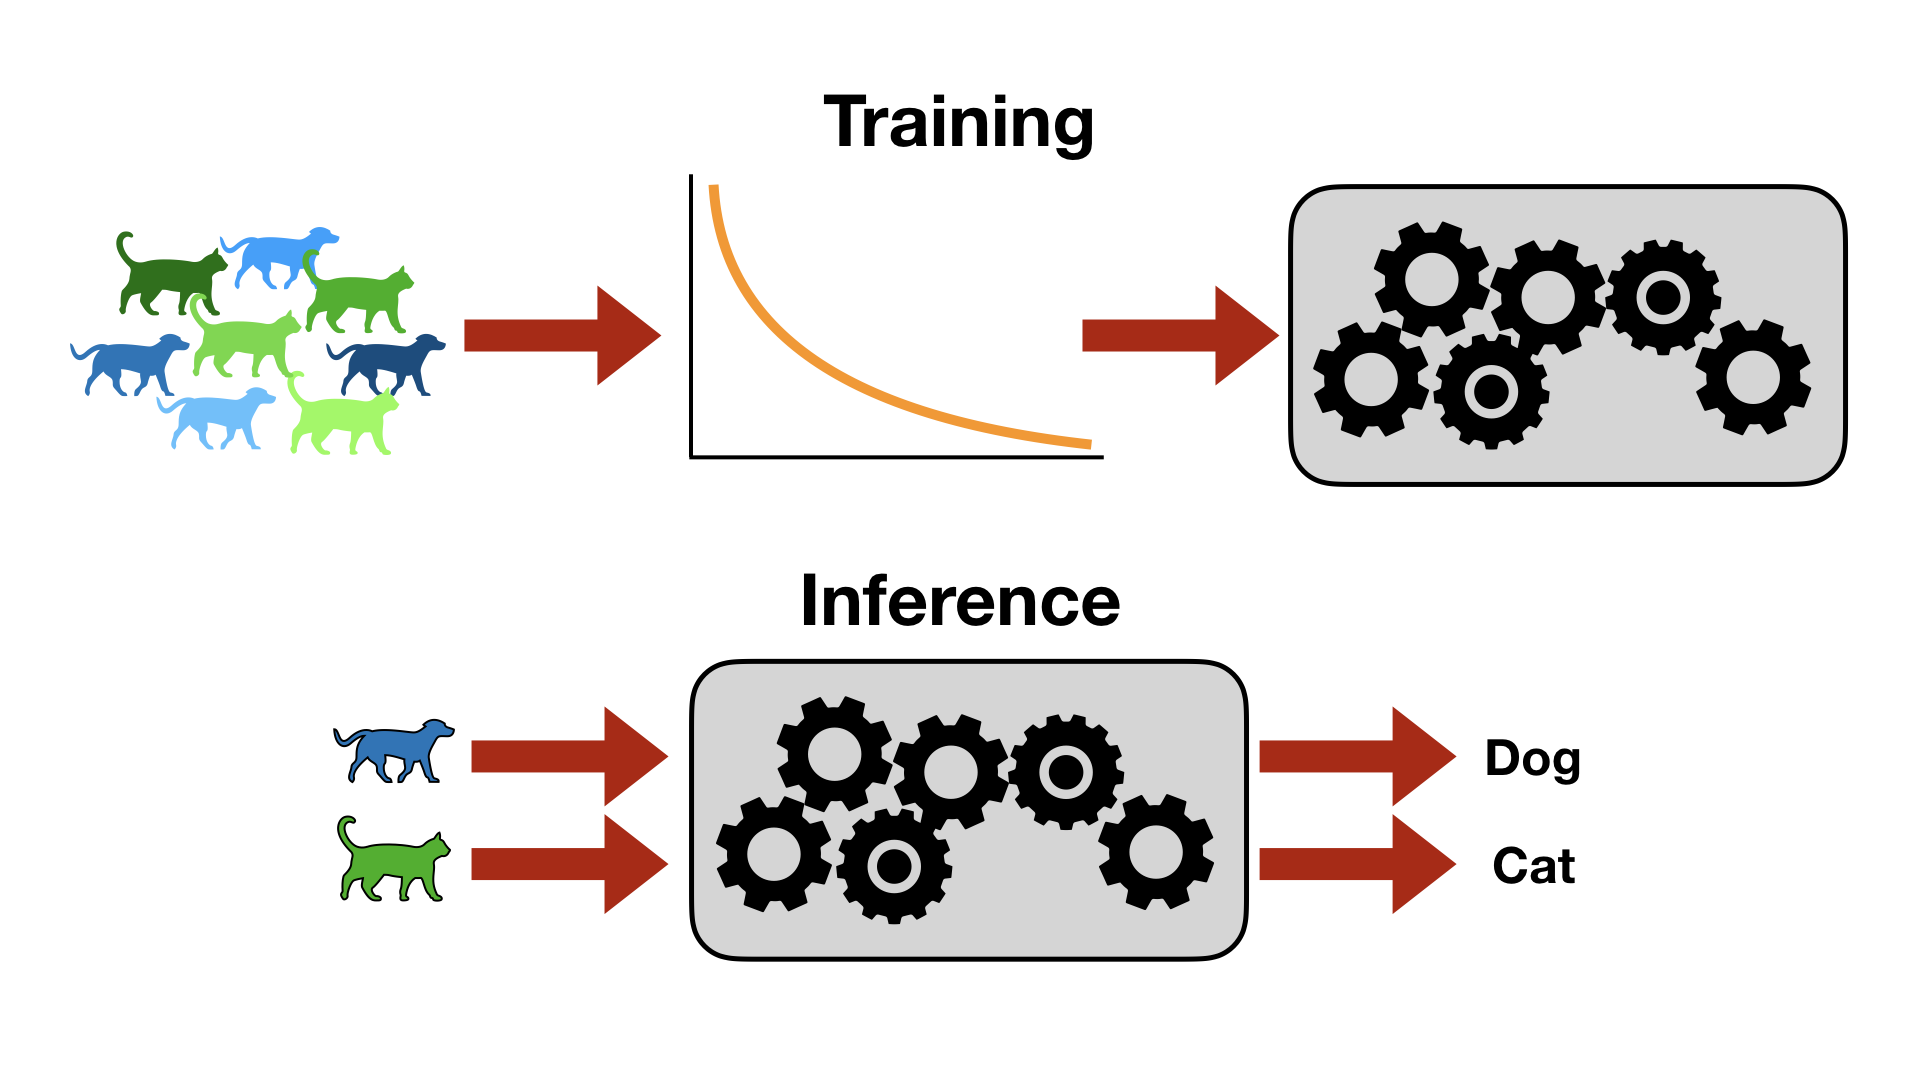
\includegraphics[trim={0 3cm 0 3cm},clip,width=0.95\textwidth]{diss/1_intro/figs/dl.png}
    \caption[Modern machine learning pipelines]{Machine learning training and inference visualization.}
    \label{fig:dl}
\end{figure}

% \textit{Explainability} can be seen as identifying important features of the input, as well as parts of the model (parameters) that ``light up`` for that input. \textit{Fairness} can be evaluated via measures over subsets of the data that correspond to specific groups. 

\begin{mdframed}[style=MyFrame]
\em 
\textbf{This thesis} focuses its main efforts on identifying these important subsets of model, feature, and sample space, to enable answering questions necessary for mainstream adoption of machine learning methods.
\end{mdframed}

% In this dissertation, we explore the sizes of these models, samples, and datasets, and 
% analyze under what situations 
% a smaller \textit{subset} of them may be sufficient or important
% for questions that run parallel to standard performance and accuracy measures.

Let us step a bit deeper into a basic illustrative example. In order to ease understanding, we can first begin with a basic formulation of learning methods, from which the questions above can take specific forms. 
Learning methods typically  try to identify a function mapping (model) that is able to complete a specific task at some high level of profficiency.
% In Figure~\ref{fig:dl}, a model is trained using examples of classification task (top), in order to accurately predict the class of a newly provided input (bottom).
% \begin{figure}
%     \centering
%     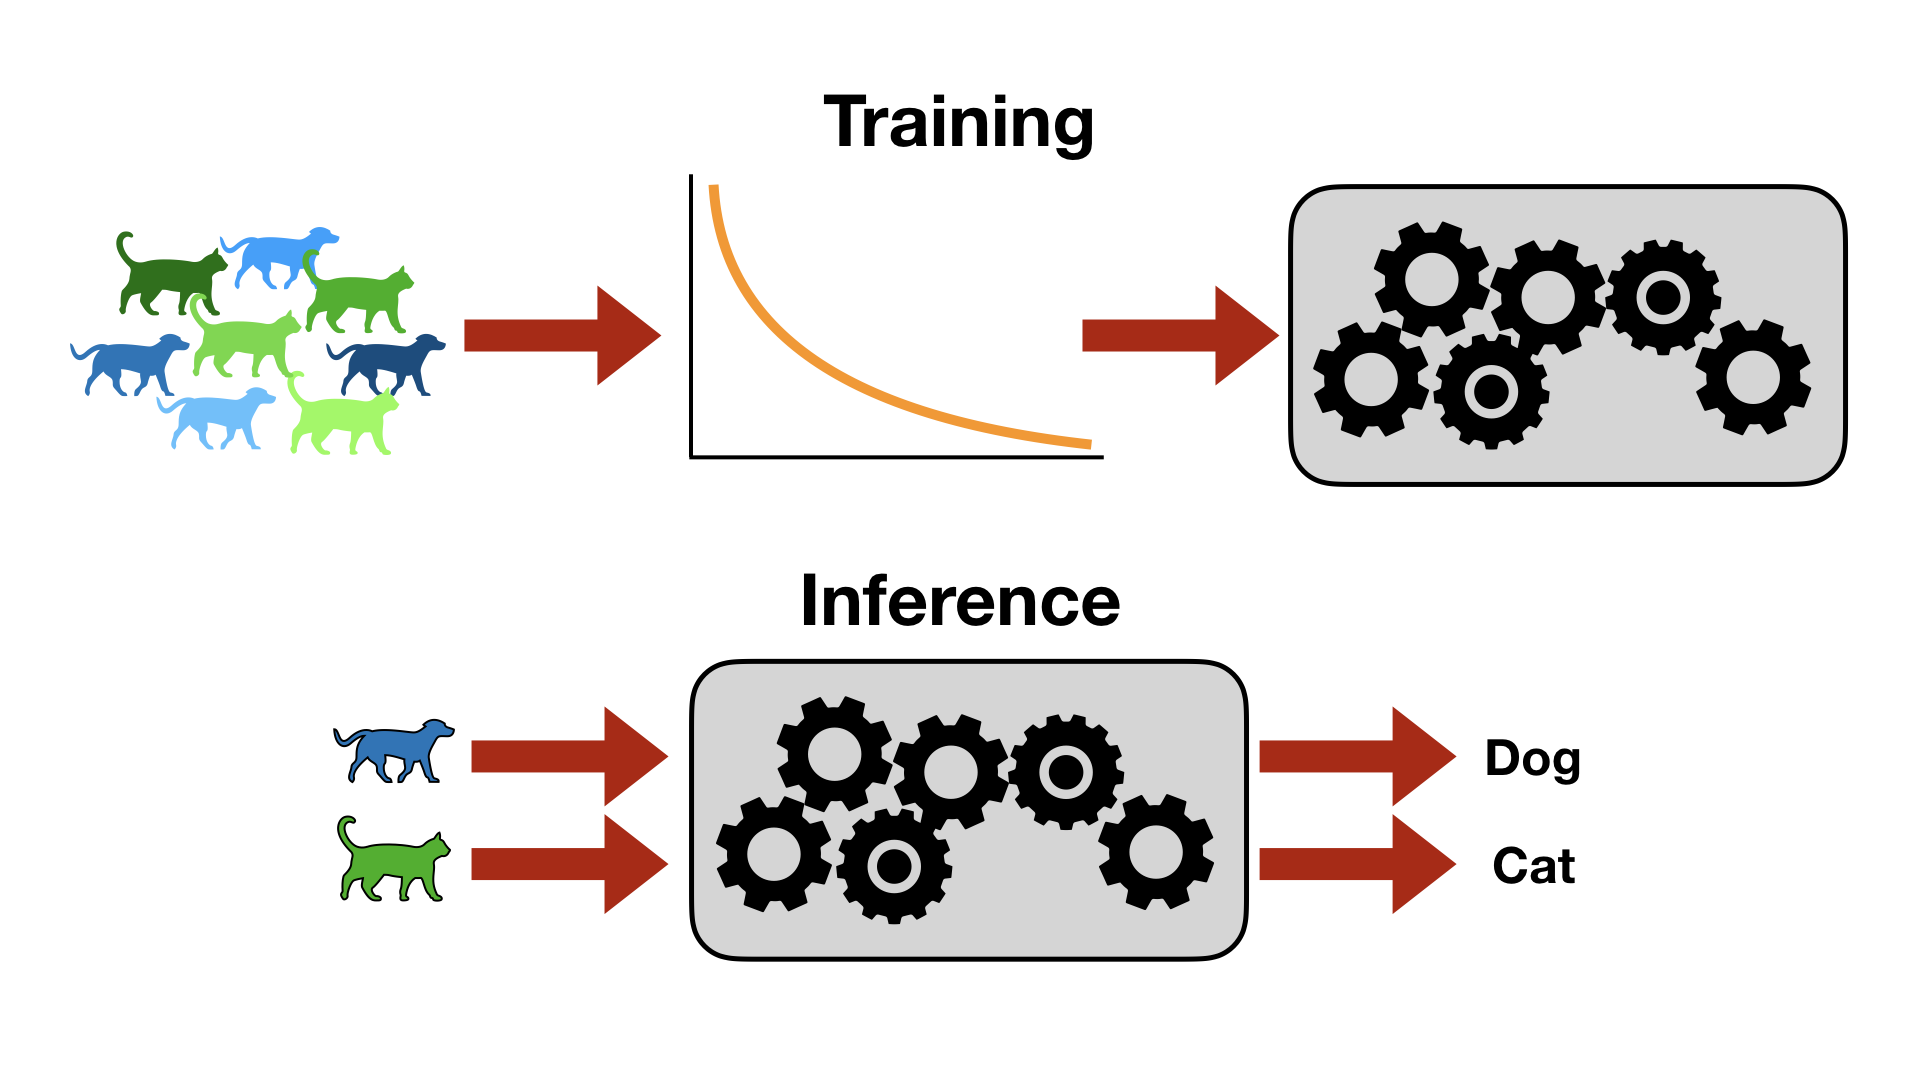
\includegraphics[trim={0 3cm 0 3cm},clip,width=0.95\textwidth]{diss/1_intro/figs/dl.png}
%     \caption[Modern machine learning pipelines]{Machine learning training and inference visualization.}
%     \label{fig:dl}
% \end{figure}
Say we have some dataset comprising of sample pairs $(x,y)$, where we wish to predict $y$ from $x$.
Our prediction, say $\hat{y}$, might be the output of some unknown function $f$ that we attempt to learn from training data. 
Let our approximation to this function be $\hat{y}:=\hat{f}(x)$.
This can take many forms, 
based on assumptions and prior information we may have on the relationships among the data. 
Consider the simple \textit{linear} case,
where we want to learn some parameter $w$ such that $y = w\cdot x$. 
Given $n$ sample pairs $(x_i,y_i)$ indexed by $i$, traditional statistics and optimization literature yield the following \textit{least squares} problem formulation, where we want to minimize the ``squared error'' between the observed values $y_i$ and the predicted $\hat{y}_i:= w\cdot x_i$:
\begin{align}\label{eq:lq}
\hat{f}:=\hat{w} = \mathop{\arg\min}_{w} \sum_{i=1}^n (y_i - w\cdot x_i)^2
\end{align}
This formulation expands without much change to a multi-dimensional form of the input $x$ and respectively, $w$: the canonical case where a number of features, or \textit{covariates} (e.g., symptoms), are used together to predict the outcome (e.g., diagnosis). 
If we are interested in which features of $x$ are important, we can look at the relative values of the learned ``weights'' $w$. In this simple setting, the importance of a feature (say $x^j$) can be exactly determined by the importance of the parameter ($w^j$).
A weight value far from zero may indicate that corresponding feature is important for diagnosis.
% If instead we are interested in which samples are most important, we can use existing methods for sample reweighting or methods that use standard assumptions to efficiently identify important subsets.

In this case and others, traditional statistical learning methods 
have been studied 
for many decades.
Linear regressors, decision trees, and support vector machines
have all been analyzed under these lenses.
% ,
% and as the modern machine learning community
% has returned to these questions recently,
% so has a renewed interest in their methods of analysis.
New research focuses
particularly on the differences
associated with moving from classical \textit{under-parametrized} models to
modern (deep) \textbf{over-parameterized} models: where
the model size vastly outnumbers the number
of input samples.
% , and may even be comparable to 
% the \textit{entire sample space.}
Methods for estimating the number of samples needed,
the time to learn a particular task,
and the generalization ability 
all require new perspectives in this regime.
While nascent, this research
attempts to fill the gap between
statistical and deep models to enable similar measures of sample influence, feature importance, and model understanding. 

\paragraph{A full picture.}
Let us expand our notation from the example above to consider this more general framing.
Consider a dataset $X:=\{x_i\}_{i=1}^n$ of size $n$ where each data point $x_i$ in the set $X$ is drawn from some underlying distribution over the domain $x_i \sim \cX^d$, 
with domain dimensionality (number of features) $d$.
A model $f$ is fit using a parametrization $\theta \in \Theta$,
with $\Theta$ the space of possible parametrizations (models) with some intrinsic dimension $p$. 
%While all three of these problems are closely related, they require different approaches. 
Generalizing the least squares``error measure'' from Eq.~\eqref{eq:lq} to an arbitrary \textit{loss} $\ell$, we have
\begin{align}\label{eq:learning}
    \hat{f}:=\hat{\theta} = \mathop{\arg\min}_{\theta\in\Theta} \sum_{x \in X} \ell(f_\theta(x_i))
\end{align}
From an analysis perspective, 
we might be interested in any one of 
(a) subsets of input features $\cC \subseteq \cX$ that are important for the downstream task,
(b) associating model subsets $\cP \subseteq \Theta$ with specific inputs or groups of inputs, or 
(c) subsets or subgroups of samples $S \subseteq \{X\}$ that are sufficient or representative of the entire dataset.

Crucially, an uninformed search for a subset is computationally infeasible. For a superset of size $n=|X|$, The set of all subsets is the power set, with a size of $2^{n}$! If an identification procedure requires looking over all of these and choosing a ``best'' one by some metric, the procedure will be limited to very small supersets.
Efficient methods have been developed in each of the three contexts above to avoid this exponential search.

\begin{figure}
    \centering
    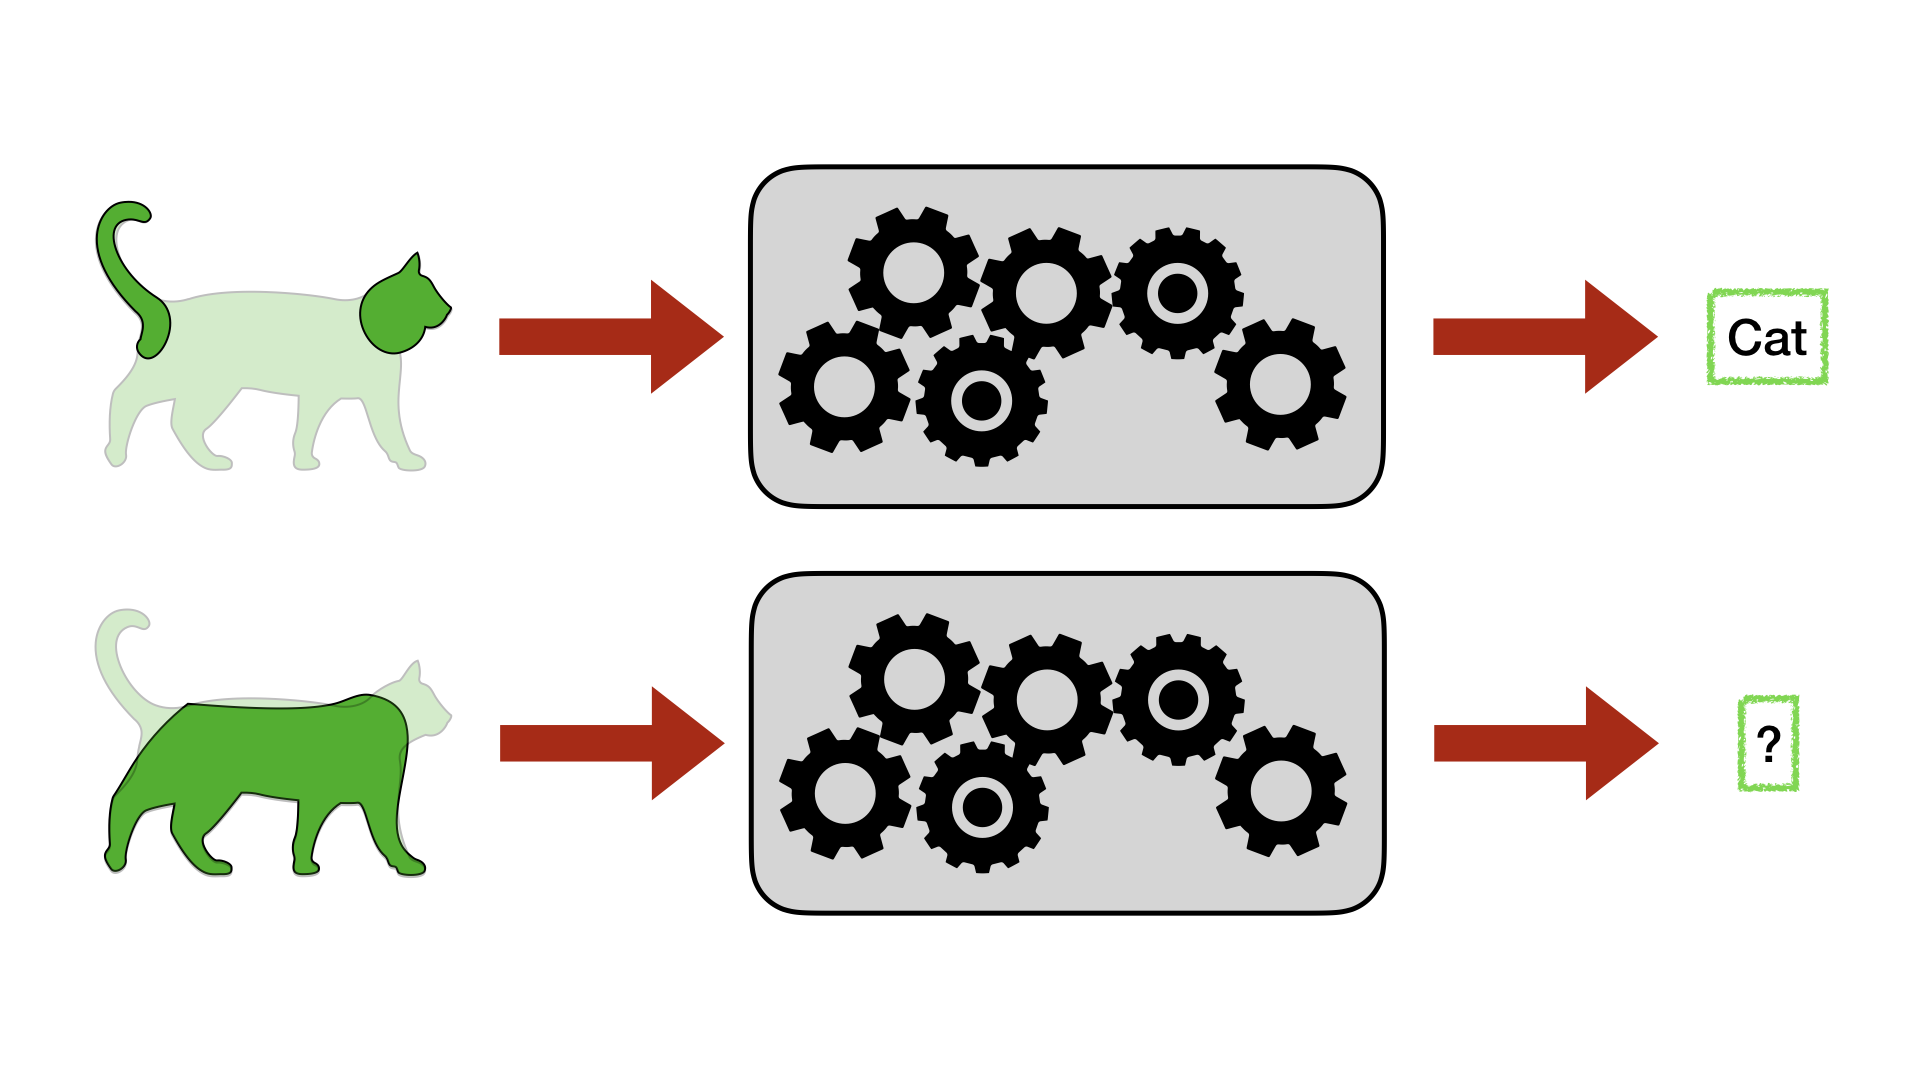
\includegraphics[trim={0 3cm 0 3cm},clip,width=0.9\textwidth]{diss/1_intro/figs/feat_select.png}
    \caption[Visualization of feature selection]{An example of identifying specific features important to the learning task.}
    \label{fig:feat_select}
\end{figure}
\paragraph{Feature Selection.} 
With more complex models $f$ compared to the linear case above, newer ``black-box'' methods have been developed for identifying important features. From the more pure statistics side, scan statistics~\citep{scanstat,scanstatlrt} allow for a structured ``scanning'' over the input space, skipping subsets unlikely to provide additional information for the measure of interest.
Further on the deep learning side, adaptations of sensitivity analysis, via noise addition and perturbations have found success~\citep{yeung2010sensitivity,zhang2015sensitivity}, alongside activation mapping~\citep{cam,selvaraju2017grad}.
These methods typically generate an analagous ``weighting'' over the input space, identifying features most salient for the specific task (Figure~\ref{fig:feat_select}).

\begin{figure}
    \centering
    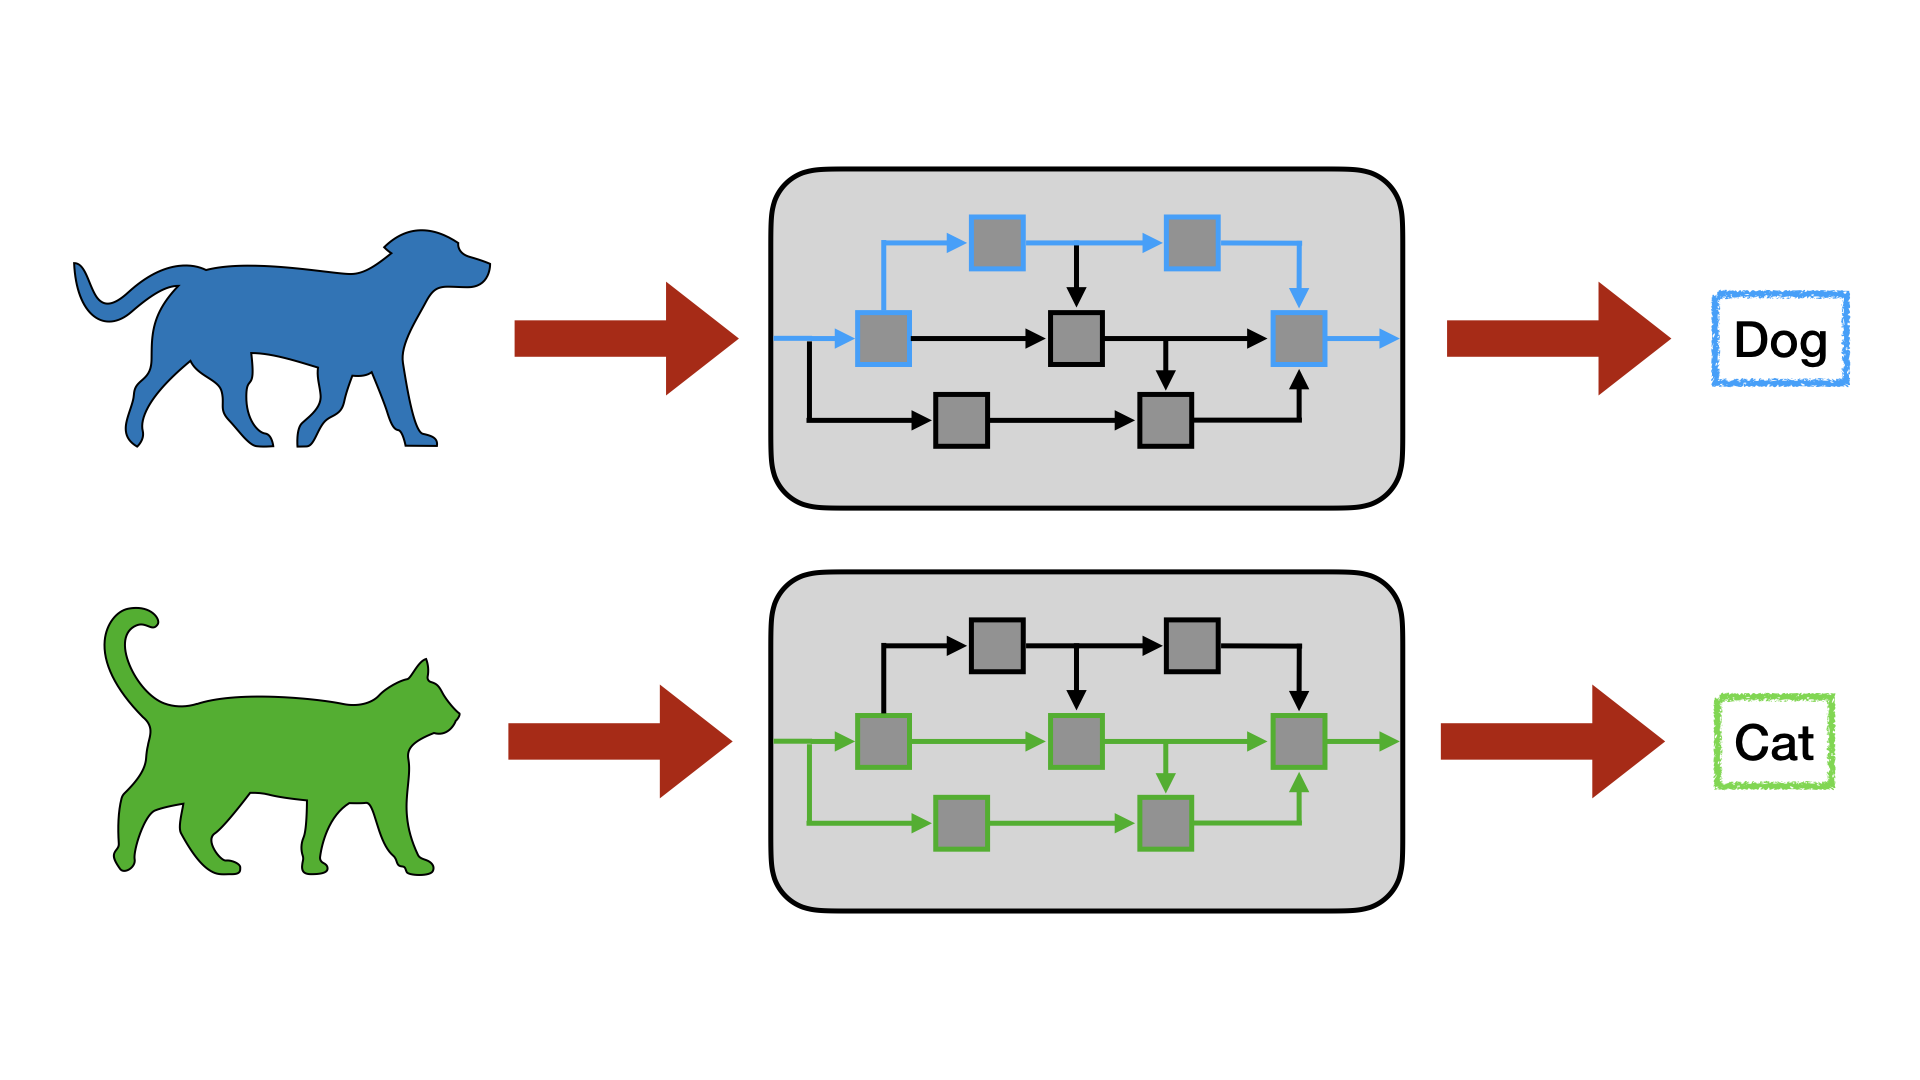
\includegraphics[trim={0 3cm 0 3cm},clip,width=0.9\textwidth]{diss/1_intro/figs/param_select.png}
    \caption[Visualization of parameter selection]{An example of identifying specific parameters important to the learning task.}
    \label{fig:param_select}
\end{figure}
\paragraph{Parameter Selection.} 
Selection in the model space generally takes two forms. First, as a prior, restriction, or assumption over the model space, and second, as a post-hoc method for an ``explainable'' proxy.
Regularization, sparsity, and gating methods are often used independent of the type or size of the model, to encourage the solution to fall within a specific region of the model space.
% In non-deep settings these methods come with strong theoretical guarantees. 
The theoretical underpinnings of these methods in deep learning are still being actively researched~\citep{hardt2016train,jacot2018neural,neyshabur2014search}, but the methods have nonetheless been effective in practice. 
On the post-hoc side, of particular interest are the parameters relevant to specific regions of the input space \textit{after} training (Figure~\ref{fig:param_select}). Here, recent analysis of deployed networks has shown this to be true~\citep{bau2017network,fong2018net2vec}, and current work continues to explore these network regions to aid in interpretability and explainability.

\paragraph{Sample Selection.} Many methods have been developed for outlier detection within training or testing sets~\citep{huang2020feature,ren2019likelihood} \textit{after} training, as well as methods for understanding sample influence~\citep{koh2017understanding,golatkar2020eternal,huang2020feature} . ``In-the-loop'' methods for accounting for ``outlierness'' behave similarly to accounting for group or individual fairness while training~\cite{mehrabi2021survey}. Unfortunately, once samples are identified in some manner, post-hoc adjustments to a trained model are generally very difficult. Recent work has focused on ``unlearning'', or removing a sample's influence on a model without retraining. If specific samples can be uniquely identified, performance and privacy reasons may require these specific interventions to reduce the ``influence'' of that sample subset.
\begin{figure}
    \centering
    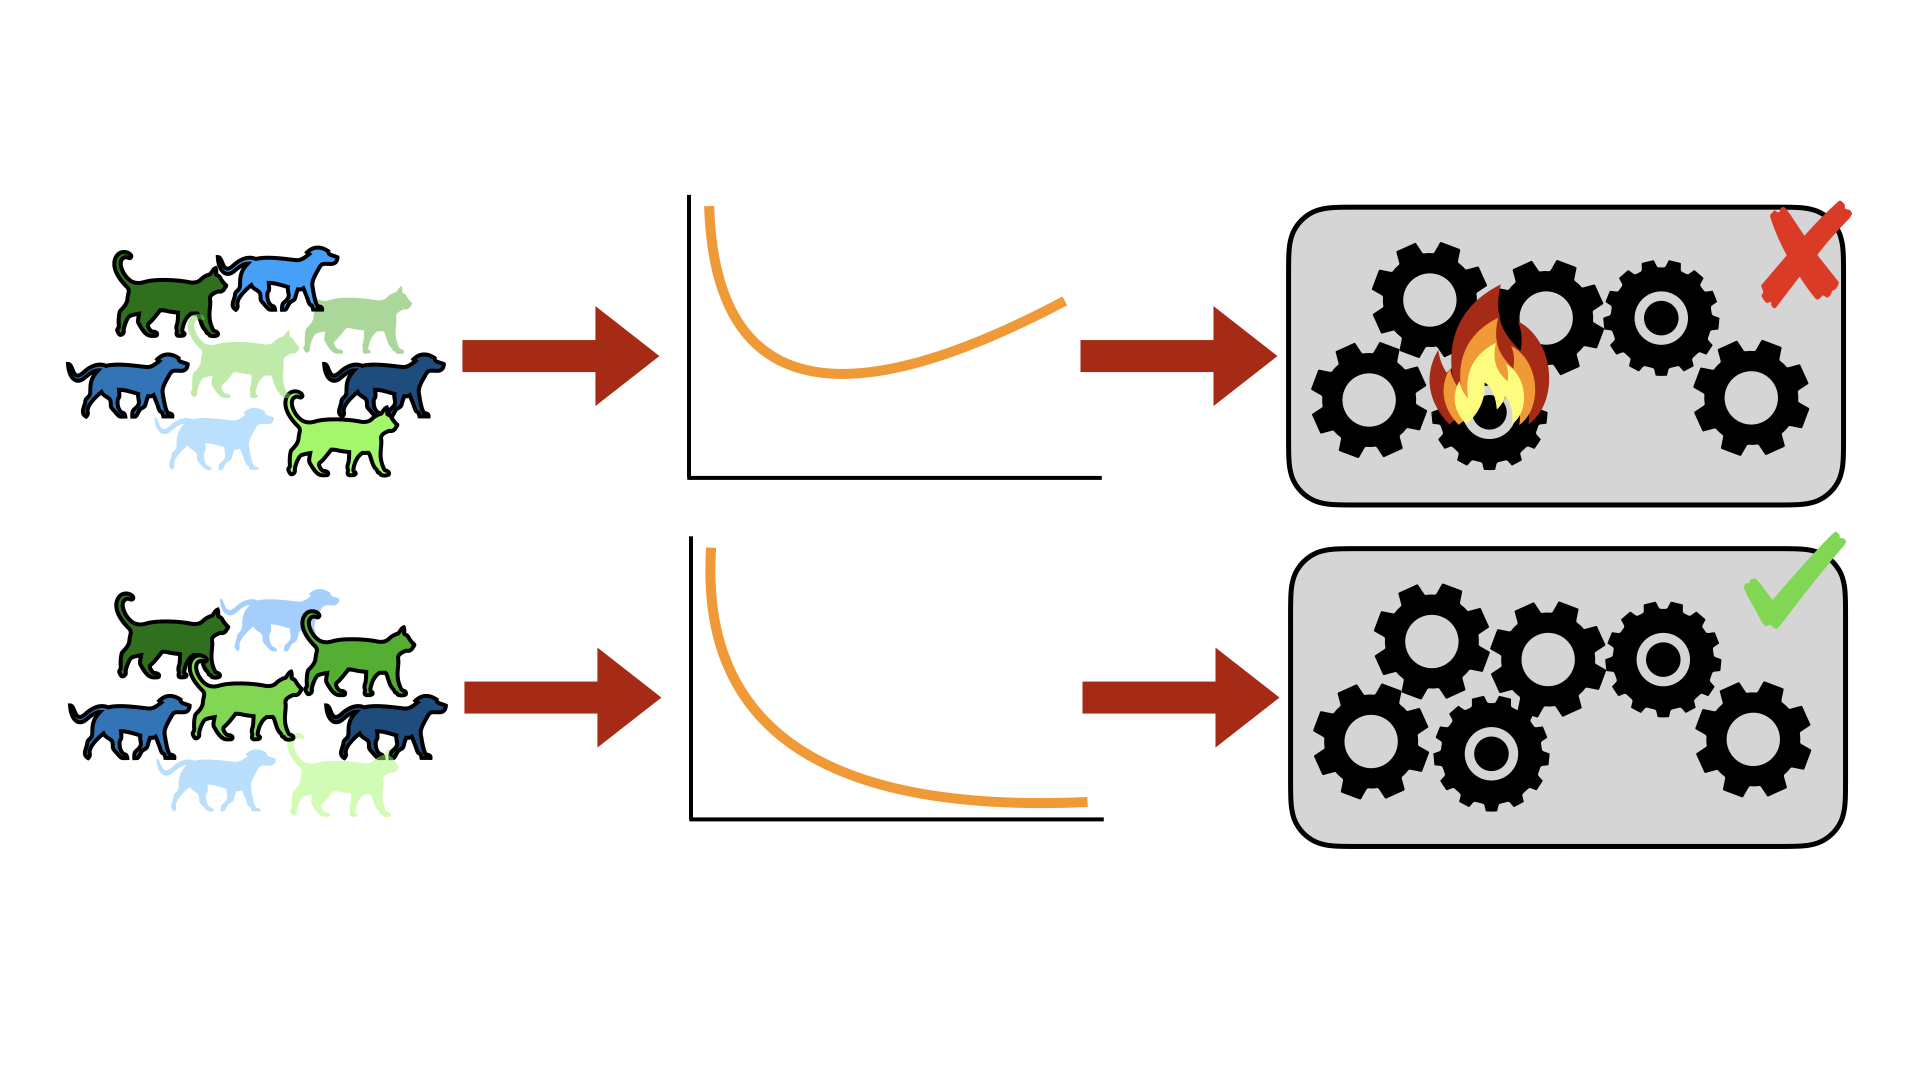
\includegraphics[trim={0 4.5cm 0 4cm},clip,width=0.9\textwidth]{diss/1_intro/figs/sample_select.png}
    \caption[Visualization of sample selection]{An example of identifying specific samples important to the learning task.}
    \label{fig:sample_select}
\end{figure}


\begin{mdframed}[style=MyFrame]
\textbf{ Thesis Goal: }
\em Identify, construct, and evaluate methods for \textbf{efficient} subset identification in modern machine learning feature, model, and input spaces.
\end{mdframed}

\section{A Few Motivating Examples}
Consider a traditional machine learning classification task in which we would like to predict whether an individual has a specific disease condition based on a medical resonance image (MRI) scan of their brain. Our input feature $x$ may consist of a 3D-array of values in $\RR^{\cI\times \cJ\times \cK}$ measuring some intensity of the imaging modality at each voxel, indexed by a tuple $(i,j,k) \in (\cI,\cJ,\cK)$.
Our outcome variable $y$ may simply be a binary label of whether the input scan has been labeled by a radiologist as one demonstrating typical disease characteristics.
Using an off the shelf 3D convolutional neural network with adjustments to match our input size, we can very quickly set up and train a system to predict disease presence with a high degree of accuracy.

\paragraph{Example 1.}
With a prediction for a specific scan, or predictions over a number of scans, we might be interested in identifying which regions of the brain are most important for diagnosis. These regions, $R \subset \cR:=\RR^{x\times y\times z}$, can be specific groups of pixels in the image that may correspond to known functional networks. Methods such as attention and class activation maps may work here, but there are a few issues. The number of samples available to learn a model is very small compared to the both the dimension of the input and the number of parameters in the model, i.e., $n \ll p$ and $n \ll d$. Thus it is very easy to overfit, and for areas of interest to be associated with intricacies of particular input data rather than true, real differences defined by the disease.

Furthermore, recent medical imaging studies have moved past simple difference detection: trends over time, and the ability to predict {\em future} disease development have by far become the setting of most interest.
Given an image of a healthy individual, is it possible to predict what their scan, or their future disease diagnosis, may be up to 10, 20, or more years in the future?
If a number of scans have been collected over some timeframe, can the \textit{trajectory} of the individuals' development be extrapolated to estimate progression?
As traditional models extended for temporal analysis grow in both size and complexity,
a number of subproblems explicitly related to model and input subspaces arise. In this thesis we address two such problems: \textbf{statistically rigorous identification of temporally evolving subsets}, and \textbf{characterizations of deep models that enable efficient training of recurrent models with large scale time-varying data}.
    
\paragraph{Example 2.}
With the rapid growth of AI and machine learning applications has come valid concerns regarding both guarantees of privacy.
Recent technology legislation has made the importance clear in all aspects of data use,
and particular projects and groups have demonstrated that machine learning is not independent of
this need \citep{Exposing}.
A new issue raised within this intersection is the ``right to be forgotten".
If a model has been trained with a particular users' data, 
they should have some recourse or right
to both remove their data from the training set,
and also know that the model has not learned from their data.
On the surface, this poses a significant problem for model builders
and organizations that spend large amounts
of time and resources in 
training deep learning models.

In the medical imaging example above this is especially important: with fewer samples it is more likely that information about any particular one could ``leak'', and the model's performance may degrade significantly as a relatively large percentage of it's training data is removed.
Thus tailored methods must be developed to ensure both privacy and performance, without requiring full retraining.
As we will see, 
\textbf{identification of model parameter subsets}
that are particularly important
for a particular sample's influence
in a model enables \textit{efficient machine unlearning}.

\paragraph{Example 3.}
From an alternative perspective, we may want to identify specific samples rather than have them specified a priori.
Traditionally a rigorous area of study under classical statistics, outlier detection and accounting have become a subfocus for many within the machine learning community as well \citep{golatkar2020eternal,golatkar2020forgetting,huang2020feature,ren2019likelihood}.
While subgroups of input samples may be outliers, it is more often the case that they represent known heterogeneity within the data. 
These differences may be marked using 
group information known a priori, and 
most learning tasks aim to learn tasks
in a \textit{subgroup-independent} manner.
In our disease prediction model above,
these groups could simply be stratified by the type of scanner used to acquire the image, but it could also
be a systematic difference correlated with some protected attribute. {\color{red} sentence about original brain atlas for registration being eurocentric}
This can directly lead to disparate performance and results on \textit{all} individuals outside of that group.
Optimization and regularization methods with this focus come under the umbrella of model fairness.
However, many existing methods do not scale well to larger models or as the number of subgroups grows, as is often the case when intersections of protected classes must be considered. Here we identify and construct a particular solution for \textbf{groupwise fairness that enables efficient in the loop fairness regularization}.

% What features are most important for prediction?
% Which samples were most important for my training?
% Can we understand when a model is certain or uncertain about its output?
% Are there layers in my network that have learned a particular subtask?
% Questions of robustness, bias, influence, fairness, and importance have become central questions to contemporary machine learning research \citep{doshi2017towards,mehrabi2021survey,amodei2016concrete}.
% machine learning, etc.

% Feature selection in the case of
% typical regression or classification 
% takes some form of learning parameters $\theta$ that allow for $\hat{y} = f_\theta(x)$ to be close to the true outcome of interest $y$.
% While forms of data $X := (x,y)$ may simply be continuous and real-valued, modern machine learning has greatly expanded formulations of the classical learning problem to include a wide variety of structured learning problems~\citep{nowozin2011structured}. 
% Consider the case when a high-dimensional input is used to predict an output with a highly-parametrized model. 
% Once learned, obvious questions arise as discussed above: are there specific low-dimensional spaces in either the input or the model space that are most important or necessary for the global learning problem of interest? Are there specific subspaces associated with particular subproblems of the global problem?
% The machine learning literature has come up with a number of ways to identify analogs of these spaces, 
% including extensions of sensitivity analysis to deep learning~\citep{yeung2010sensitivity,zhang2015sensitivity}, and constructing and identifying nonzero model subsets via particular model choices such as activations~\citep{selvaraju2017grad} and regularizers.
% In classical settings these are well understood: decision trees naturally provide ease of interpretibility via the information used to choose splits, and both linear and kernel support vector machines have been analyzed to provide for measures of sample importance via distances to the margin as well as feature importance via weights defining the learned hyperplane~\citep{Mitchell97}.
% Attention and saliency maps have emerged as popular new methods,
% given their ease of implementation and interpretation~\citep{sutskever2014sequence,vaswani2017attention,selvaraju2017grad}.
% By learning dimensions of a given input that are particularly important, either in a hard (binary) or soft (continuous weighting) manner, model builders are better able to understand and interpret what a model has learnt.
% The specific ideas of attention notwithstanding, many of these existing methods are far removed from traditional hypothesis testing frameworks.
% While some work has begun in this direction~\citep{tansey2018black},
% there remains a gap in direct identification of subsets and structures in these spaces that can be defined in statistically rigorous manners.

% \begin{figure}
%     \centering
%     \includegraphics[width=0.5\textwidth]{example-image-a}
%     \caption[A simple subset selection example]{\color{red} Identifying and selecting in MRIs, subset, sample, model ID.}
% \end{figure}

% \paragraph{A specific example.} 

% ------------------------------------------

% below here will be moved and arranged with the "selection" sections and here if relevant

% ------------------------------------------

% While attention can be directly applied to the network in order to identify ``hotspots" in the input space relating to the learned classification task, 
% given the high-dimensional nature of the input
% and the relatively small sample size 
% associated with medical imaging data, 
% it is very likely that an area of interest identified
% may be an intricacy of the training samples used rather than truly a region of disease signal.
% Class activation maps (CAMs) may be unclear, and can often associate with image artifacts unrelated to the scientific task~\citep{adebayo2018sanity}.
% Methods of generalization may help to increase confidence in identified regions, but statistical guarantees often remain out of reach.

% Furthermore, most recent problems associated with medical data have moved past simple difference detection: trends over time, and the ability to predict {\em future} disease development has by far become the setting of most interest.
% Given an image of a healthy individual, is it possible to predict what their scan, or their future disease diagnosis, may be up to 10, 20, or more years in the future?
% If a number of scans have been collected over some timeframe, can the \textit{trajectory} of the individuals' development be extrapolated to estimate progression?
% As traditional models extended for temporal analysis grow in both size and complexity,
% a number of subproblems explicitly related to model and input subspaces arise. Here we address two such problems: \textbf{statistically rigorous identification of temporally evolving subsets}, and \textbf{characterizations of deep models that enable efficient training of recurrent models with large scale time-varying data}.

% A sample's particular influence on model parameters aside, the identification of influential samples or subsets of samples more generally is of independent interest. 
% Traditionally a rigorous area of study under classical statistics, outlier detection and accounting have become a subfocus for many within the machine learning community as well \citep{golatkar2020eternal,golatkar2020forgetting,huang2020feature,ren2019likelihood}.
% While subgroups of input samples may be outliers, it is more often the case that they represent known heterogeneity within the data. 
% These differences are typically marked using 
% group information known a priori, and 
% most learning tasks aim to learn tasks
% in a \textit{subgroup-independent} manner.
% Optimization and regularization methods with this focus come under the umbrella of model fairness, and instead of identifying and boosting independences within the model or data, we aim to minimize them.
% However, many existing methods do not scale well as the number of subgroups grows, as is often the case when intersections of protected classes must be considered. In the sequel we identify and construct a particular solution for \textbf{groupwise fairness that enables efficient in the loop fairness regularization}.

\begin{mdframed}[style=MyFrame]
\em 
Here we focus our effort on identifying these important subsets of model, feature, and sample space for feature association, model size reduction, model unlearning, and, fairness. Specifically, taking advantage of both existing statistical and geometric methods, we develop new methods for localizing subsets in a range of settings from hypothesis testing to deep learning.
\end{mdframed}

\section{Thesis Scope and Contributions}

We explore the intersections of classical statistical and geometric constructions with modern machine learning methods. 
Figure~\ref{fig:scope} shows the overall scope projected along three axes: feature, parameter, and sample spaces.
Below we briefly introduce the main problems studied in this thesis.
\begin{figure}[!ht]
    \centering
    % \includegraphics[width=0.99\linewidth]{scope.pdf}
    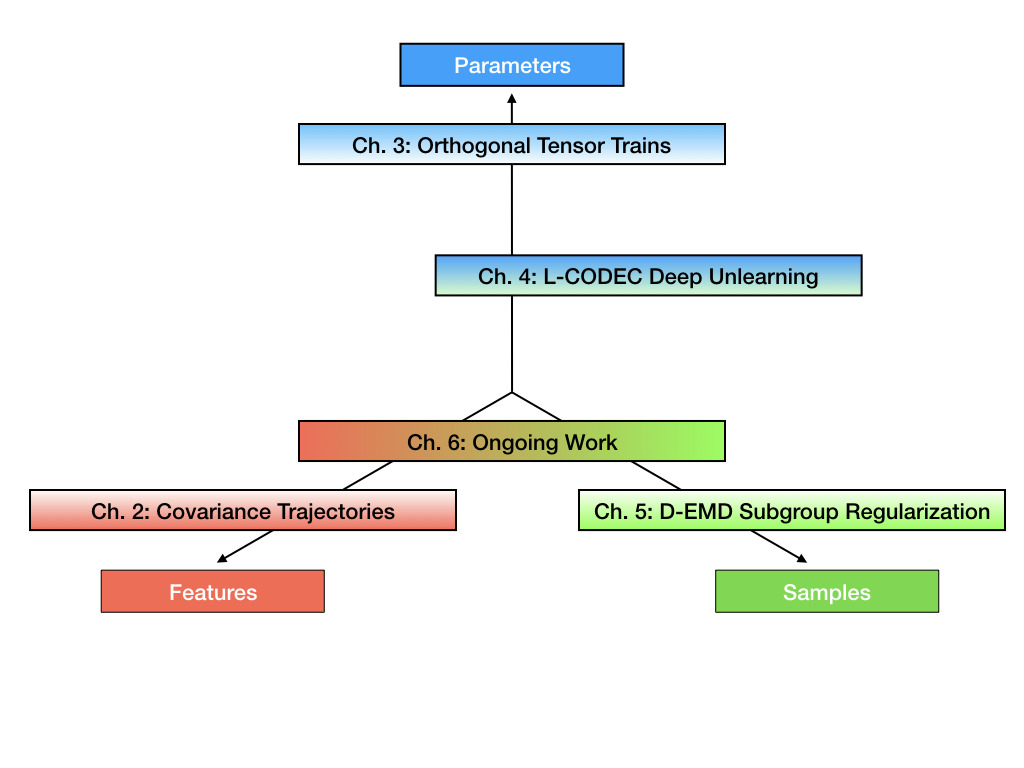
\includegraphics[width=0.95\linewidth]{diss/1_intro/figs/thesis_scope.png}
    \caption[Thesis Scope]{Thesis scope, projected over three representative axes. {\color{red} update chapter numbers shift by 1}}
    \label{fig:scope}
\end{figure}

\subsection{Second-Order Modeling and Group Difference Analysis over Time}

Recent results in coupled or temporal graphical models offer schemes for estimating the relationship structure 
between features when the data come from
related (but distinct) longitudinal sources. A novel application of these ideas is for analyzing group-level differences, i.e., in identifying if {\em trends} of estimated objects (e.g., 
covariance or precision matrices) are different across disparate conditions (e.g., gender or disease). Often, poor effect sizes make detecting the \textit{differential} signal 
over the {\em full} set of features difficult: for example, 
dependencies between only a {\em subset of features} may manifest differently across groups.
We first suggest
a parametric model 
for estimating trends in the space of $\SPD$ matrices as a function of one or more covariates.
We will then generalize scan statistics to graph structures, 
to search over distinct subsets of features (graph partitions) whose temporal dependency structure may show statistically 
significant group-wise differences.
We will theoretically analyze the Family Wise Error Rate (FWER) and bounds on Type 1 and Type 2 error. 
On a cohort of individuals with risk factors for Alzheimer's disease (but otherwise cognitively healthy), 
we 
find scientifically interesting 
group differences where the default analysis, 
i.e., models estimated on the full set of features, do not survive reasonable 
significance thresholds. 
% Preliminary work on this was published in \citep{covtraj}.


\subsection{Efficient Tensor Representations for Feasible Temporal Deep Learning}

Modern deep networks have proven to be very effective for analyzing real world images.
However, their application in medical imaging is still in its early stages,
primarily due to the large dimension of three-dimensional images, requiring enormous convolutional or fully connected layers --
if we treat an image (and not image patches) as a sample. 
These issues only compound when the focus moves towards longitudinal analysis
through recurrent structures, and when a point estimate of model parameters is insufficient 
in scientific applications where a reliability measure is necessary.
Using insights from differential geometry, 
we will adapt 
the tensor train decomposition to construct networks
with significantly fewer parameters,
allowing us to train powerful recurrent networks on whole brain image volumes. 
We analyze 
the \textit{orthogonal tensor train},
and demonstrate its ability to express a standard network layer both theoretically and empirically.
We 
demonstrate its ability to 
effectively reconstruct whole brain volumes
with faster convergence and stronger confidence intervals
compared to the standard tensor train decomposition. 
We provide code and show experiments on the ADNI dataset
using image sequences to regress on a cognition related outcome.
% Preliminary work on this was published in \citep{ott}.

\subsection{Practical Unlearning via Large-Scale Conditional Independence Testing}

%With AI systems extensively using personal %data for model training, 
Recent legislation has
led to interest in {\em machine unlearning}, i.e., removing specific training samples from a {\em predictive} model as if they never existed in the training dataset. 
Unlearning may also be required due to  corrupted/adversarial data or simply a user's updated privacy requirement.
For models which require no training ($k$-NN), 
simply deleting the closest original sample can be effective. 
%However, it is not clear how such approaches can be used to unlearn 
%models that contain rich information learned from the original data.
But this idea is inapplicable to models which learn richer 
representations.
%from data. 
%Recently, optimization-based unlearning estimators have been proposed, but 5their 
Recent ideas leveraging optimization-based updates
scale poorly with the model dimension $d$,  
due to 
inverting the Hessian of the loss function. %with an overall cost of $O(d^3)$ 
%is prohibitive.
We describe
a variant of a new conditional independence coefficient, 
L-CODEC, to identify a subset of the model parameters with the most semantic overlap on an individual sample level. 
Our approach completely avoids the need to invert a (possibly) huge matrix. 
By utilizing a Markov blanket selection, 
we find
that L-CODEC is also suitable for deep unlearning,
as well as other applications in vision.
Compared to alternatives, L-CODEC makes approximate unlearning possible 
in settings that would otherwise be infeasible, 
including vision models used for face recognition, 
person re-identification 
and NLP models that may require unlearning samples identified for exclusion.
% Preliminary work on this will appear in \citep{lcodec}.


\subsection{Reducing Subgroup Fairness via High Dimensional Earth Mover's Distances}

Optimal transport has recently emerged as a useful tool for machine learning through its connections with geometry, statistical machine learning, and through practical algorithms. Existing methods that leverage optimal transport often  regularize using  a Wasserstein metric or by computing barycenters, for example. %which are effective when distributions are continuous and known, or when measures of interest are discrete.
% Our formulation allows for a discretization of continuous measures that drop in directly to classical  formulations of the Earth Mover's Distance. 
We leverage optimal transport, except that we take advantage of a recently-introduced algorithm that computes a generalized earth mover's distance.
Not only is this algorithm computationally cheaper to compute compared to existing barycentric measures, but our method has the additional  advantage that gradients used for backpropagation can be directly read off of the forward pass computation, which leads to substantially faster model training.
We provide technical details about this new regularization term and its properties, 
and 
experimental demonstrations of improved training speed over existing Wasserstein-style methods.

{\color{red}
\subsection{Understanding Latent Spaces via Conditional Independences}

The final chapter of this thesis applies some of the tools developed above in the analysis of latent spaces in recent large scale models.
% In these studies, 
% we aim to identify conditionally independent features and subjects that are particularly important to the prediction and estimation of
% key disease outcomes,
% as a function of a number 
% of demographic, neuropsychological,
% genetic,
% and imaging data collected as 
% part of an ongoing consortium 
% to understand the progression
% of Alzheimer's disease in younger, 
% asymptomatic populations.
% In what follows we present
% exploratory analysis
% on a small, easily 
% digestible subset of the available data,
% that lays the foundation for
% further analysis.
}
% This work is the most forward looking, and aims to be a stepping stone toward a rigorous 

\section{Outline}
Chapter 2 covers the essential background necessary for the developments presented in the following chapters, including specifics of graphs and hypothesis testing, as well as relevant modern methods for learning and optimization.
In Chapters 3 through 7, we describe four perspectives to address subset identification.
Chapter 3 explores and focuses on the identification of feature subsets varying over time.
In Chapter 4 we describe a method of constraining the parameter space in a particular manner
that enables more efficient large scale neural networks.
Next, Chapter 5 provides a solution to the machine unlearning problem,
enabled through a particular conditional independence parameter selection scheme, vastly reducing network update costs.
Chapter 6 ends with a unique solution to subgroup fairness, 
where we take advantage of an efficient solution to
the $d$-dimensional earth mover's problem
to regularize large models when the number of subgroups can be large.
{\color{red} Chapter 7 describes future work, focused on applying a particular solution from Chapter 5 to understanding relationships among features in latent spaces learned by large generative models.}


%%%%%%%%%%%%% 
% Some old stuff

% Significant progress in the modern development of machine learning has
% been built upon connections and patterns identified across myriad
% interdisciplinary fields of study.
% Up through the mid 2000's, 
% many of these methods were inspired by and interested in 
% highly focused and constrained problems. 
% With a reasonably sized input domain, could a model of roughly equal size be used to
% predict some output?
% Linear regressors, decision trees, and support vector machines were all answers to these questions, with their own
% varying degrees of scaling and complexity.
% These methods necessitated carefully constructed formulations with specific restrictions to the learnable function class,
% enabling straightforward analysis 
% for provable performance guarantees 
% and easy identification of critical training samples and important input features.

% Contemporary machine learning, however, has a vastly different modus operandi. 
% Driven in large part by the exponential growth of available computation via Moore's Law, \textit{deep learning} has fallen squarely in the realm of \textbf{over-parameterized} models.
% With these overparametrizations and computation capacity, the typical learning questions posed as maximizing accuracy or reducing error have largely been addressed for even large scale problems.
% As such, complementary questions have led to subfields focusing on other performance measures, such as robustness, fairness, interpretability, and explainability.
% Many solutions to these questions end up looking back at answers found for the under- or non-parametrized settings.
% While nascent, these approaches 
% attempt to fill the gap between
% statistical and deep models to enable similar measures of sample influence, feature importance, and model analysis. 
% Most notable amongst these newer approaches is that of (Self)-Attention in Neural Networks \citep{sutskever2014sequence,vaswani2017attention}.
% Other proposals 
% end up looking back at the types of analysis typical of those more classical under-parametrized or nonparametrized methods.

% Not limited to previous developments in learning or computation theory, the arguably most valuable contributions toward the exponential reduction in model error can be attributed to influences and intuitions taken
% from biology, psychology, neuroscience, and even XXX \citep{srivastava, etc}.
% Perhaps one explanation as to why this phenomenon exists may be attributed to the way in which deep learning evolved. 
% The classical learning goal of function approximation lends itself nicely to a system which allows for arbitrary complexity via simple changes (e.g., addition of neural network layers). % Foundational works building on the original neural networks particularly have taken advantage of constraining this space of functions to search over: 
% the most seminal case being those of convolutional filters for imaging data. 
% While ``constraints" of this form have helped tremendously in model performance on modern vision and language machine learning tasks (GANs, Recurrent Networks, Residual Layers, Transformers, etc.), the ability to identify \textit{subsets} of important samples, input features, and model parameters has lagged significantly behind the development of these methods.
% Recently larger interest has been taken by the community to understand and interpret models with this view, only after extremely large and opaque models have become ubiquitous.
%This lag directly explains the more recent interest in developing methods for understanding and interpreting large scale machine learning models. % DEMD
\chapter{Introduction} \label{chap:intro} 

Modern applications of machine learning in a broad range of industrial and consumer-facing systems have become ubiquitous.
Most interactions with daily technologies now intrinsically involve 
a request to some ``smart`` system in the ``cloud'', 
where those interactions range from
a request for map directions 
to simply loading a webpage.
Neural network models, and the recent advances of deep learning,
have enabled these systems that 
make such applications possible.
These models have achieved
human-level performance on learning tasks
including image classification~\citep{resnet,alexnet}, image segmentation~\citep{segmentation}, video analysis~\citep{zhang2016video}, text understanding and generation~\citep{bert,gpt}, and have slowly begun to solve more fundamental scientific problems such as protein folding~\citep{protein} drug discovery~\citep{drugdisc}, and medical diagnosis~\citep{diag}.
While this performance is largely attributed to model size,
the abundance of high quality training data
has equally contributed to real world performance,
enabling model training over millions of real world samples~\citep{imagenet,laion},
and potentially billions of synthetic samples via environment simulation~\citep{mcts}.

While deployment in some domains (recommender systems, object detection) may benefit almost unconditionally from this vastly expanded capability, rightful hesitancy has limited their widespread use in particular applications where impacts on individuals, people, or environments may be at stake.
These ``last mile'' concerns take a few forms.
% Because a completely accurate model is still out of reach, an important question that needs to be answered is: which inputs or individuals are being given incorrect outcomes, and why?
% maybe a sentence suggesting unlearning/removal
In mission critical applications such as medical diagnosis, 
the impact of an error can be extremely large,
even if a misprediction happens extremely infrequently.
Additionally, large scale model training and architecture search
can require exorbitant amounts of energy producing high emissions,
and their scale can limit market participants
to only large actors with vast existing resources.
The accessibility and effectiveness of these models can also vary significantly based on the training data, and disparate outcomes can be exacerbated by existing social inequity.

While existing human or ``natural'' systems that these models aim to assist are not perfect, 
our real world has developed norms and regulations that 
enable them to function.
A medical diagnosis might require a physician to explain what symptoms led them to that particular conclusion.
Energy metering and carbon taxes may be applied to limit
emissions.
Regulatory satisfaction may require 
analysis proving equal opportunity,
or that specific protected classes
are not used in decision making.
% Specifically, these can include ideas as simple as the Hippocratic Oath and medical malpractice insurance, to asking your doctor what symptoms lead them to a particular diagnosis.
These ideas are difficult to directly translate to automated machine learning systems,
but proxies have been identified that we can build upon.

These norms and regulations answer a number of questions we may also try to pose to our machine learning models.
What is the cost to learn this task?
What led to this particular outcome?
Why is this outcome different from another?
% We will explore how these questions can be formulated concretely. 

If the answer to these questions is negative or unknown,  follow-up questions all take an interesting form:
Can we learn a smaller model with similar performance? 
Can we identify the most important features? 
Which individuals or groups are being treated unfairly, and can we change that?
These questions ask us to identify a \textit{subset} of some relevant set, dependent on setting, and this identification is our focus here.

% Moving specifically to machine learning methods,
Taking a step back, let's take a look at a representative system. Figure~\ref{fig:dl} illustrates a typical learning pipeline. 
A dataset is collected and used to train a model, by minimizing the error over
those samples in the dataset (top).
A ``sample'' can be a single measured value, or it can
be a large, highly structured object with many ``features.''
The model is made up of some ``parameters'' that are 
tuned during training to learn a good predictor over the training dataset.
This model is then used to predict, or \textit{infer}, on new
data seen ``in the wild'' (bottom).
Our questions above are formally asking to identify \textit{subsets of these objects}: is a subset of the model parameters sufficient for learning? Which subset of the features are important for a prediction? Which subset of the dataset exhibit a specific attribute?
\begin{figure}
    \centering
    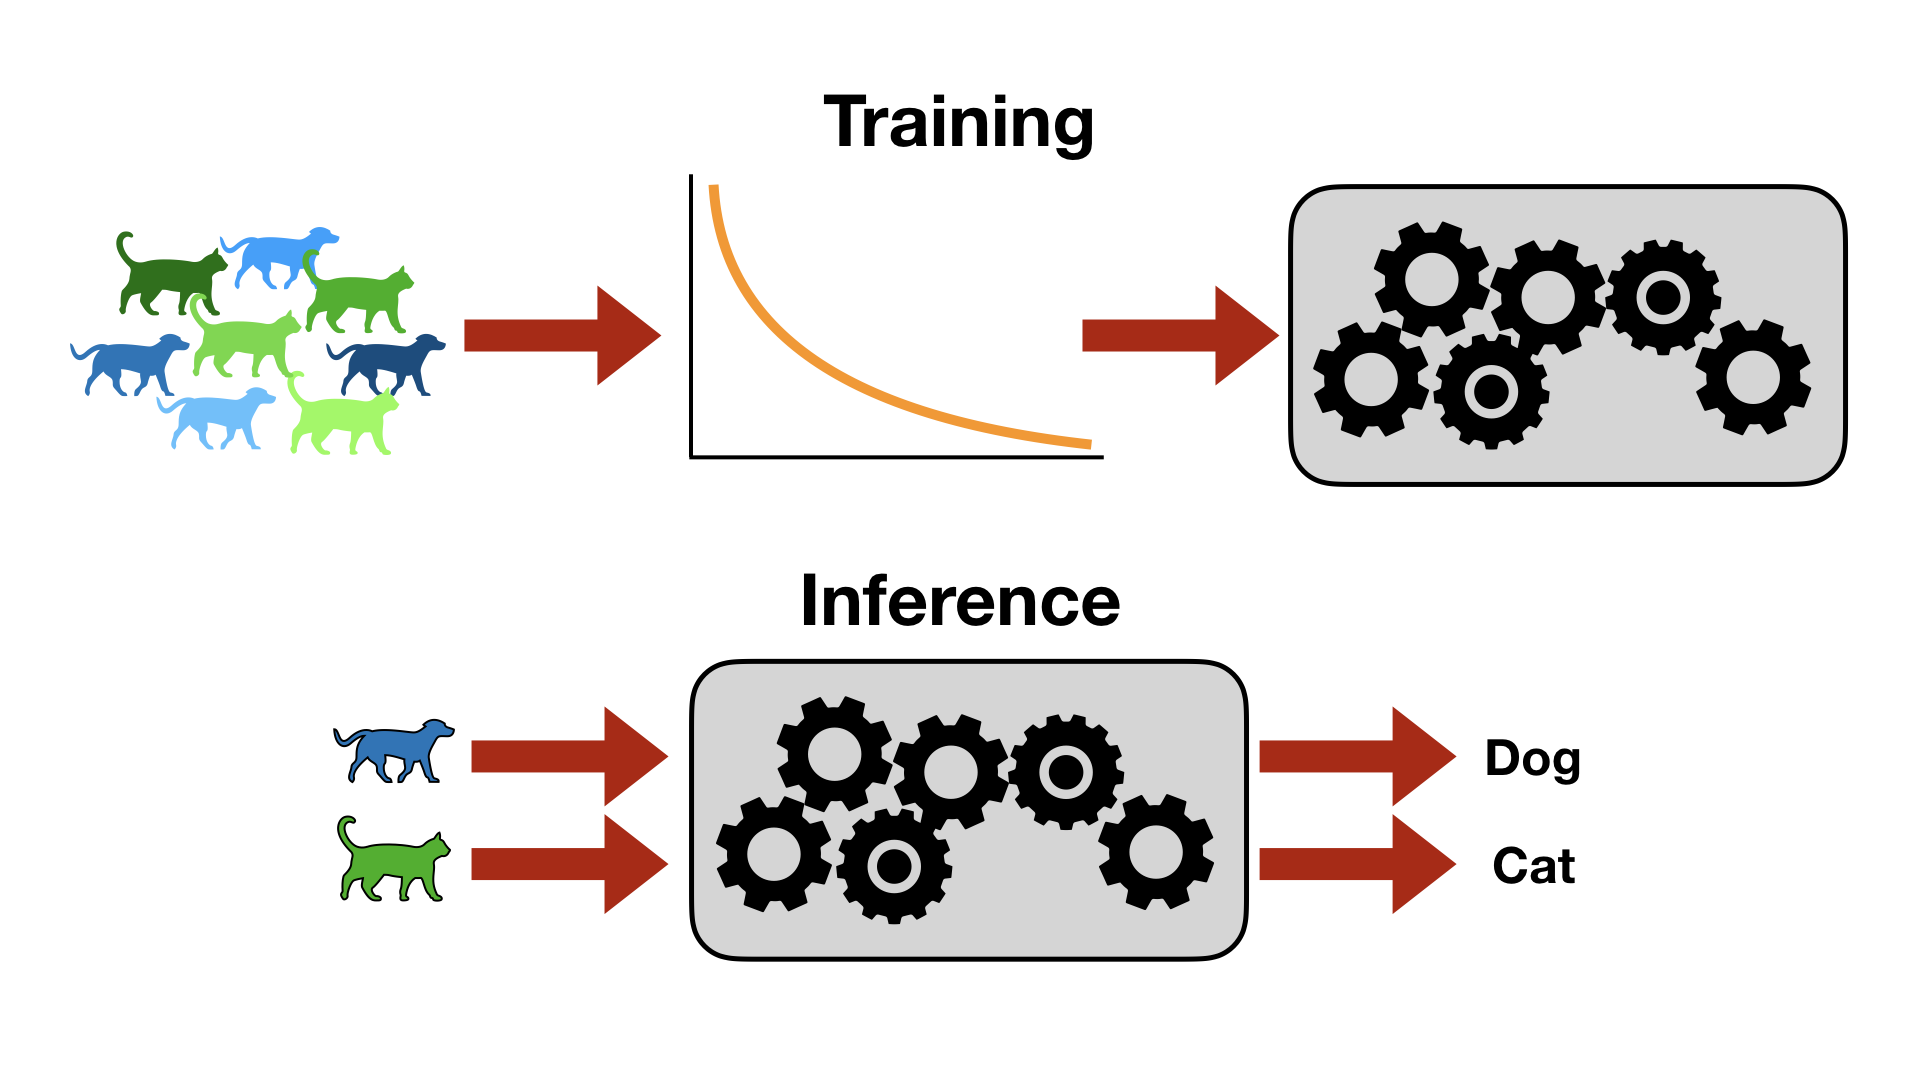
\includegraphics[trim={0 3cm 0 3cm},clip,width=0.95\textwidth]{diss/1_intro/figs/dl.png}
    \caption[Modern machine learning pipelines]{Machine learning training and inference visualization.}
    \label{fig:dl}
\end{figure}

% \textit{Explainability} can be seen as identifying important features of the input, as well as parts of the model (parameters) that ``light up`` for that input. \textit{Fairness} can be evaluated via measures over subsets of the data that correspond to specific groups. 

\begin{mdframed}[style=MyFrame]
\em 
\textbf{This thesis} focuses its main efforts on identifying these important subsets of model, feature, and sample space, to enable answering questions necessary for mainstream adoption of machine learning methods.
\end{mdframed}

% In this dissertation, we explore the sizes of these models, samples, and datasets, and 
% analyze under what situations 
% a smaller \textit{subset} of them may be sufficient or important
% for questions that run parallel to standard performance and accuracy measures.

Let us step a bit deeper into a basic illustrative example. In order to ease understanding, we can first begin with a basic formulation of learning methods, from which the questions above can take specific forms. 
Learning methods typically  try to identify a function mapping (model) that is able to complete a specific task at some high level of profficiency.
% In Figure~\ref{fig:dl}, a model is trained using examples of classification task (top), in order to accurately predict the class of a newly provided input (bottom).
% \begin{figure}
%     \centering
%     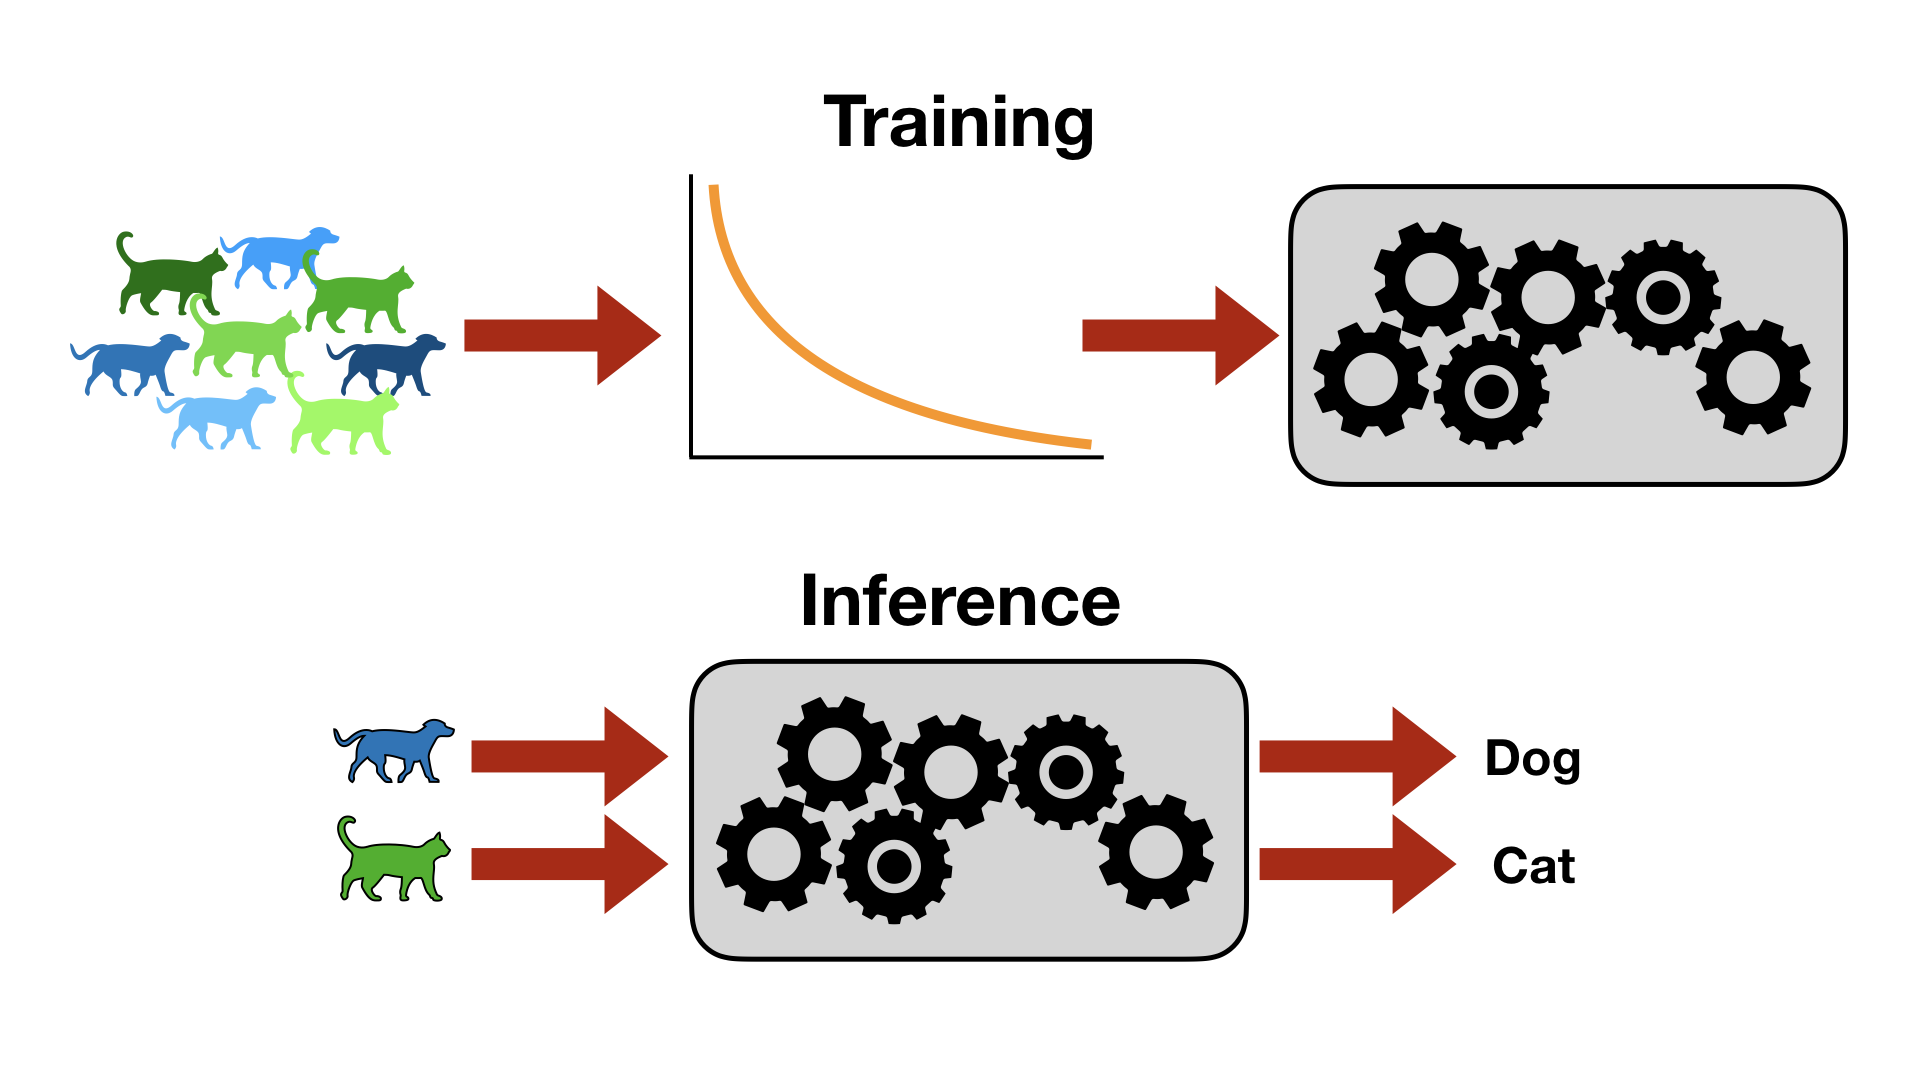
\includegraphics[trim={0 3cm 0 3cm},clip,width=0.95\textwidth]{diss/1_intro/figs/dl.png}
%     \caption[Modern machine learning pipelines]{Machine learning training and inference visualization.}
%     \label{fig:dl}
% \end{figure}
Say we have some dataset comprising of sample pairs $(x,y)$, where we wish to predict $y$ from $x$.
Our prediction, say $\hat{y}$, might be the output of some unknown function $f$ that we attempt to learn from training data. 
Let our approximation to this function be $\hat{y}:=\hat{f}(x)$.
This can take many forms, 
based on assumptions and prior information we may have on the relationships among the data. 
Consider the simple \textit{linear} case,
where we want to learn some parameter $w$ such that $y = w\cdot x$. 
Given $n$ sample pairs $(x_i,y_i)$ indexed by $i$, traditional statistics and optimization literature yield the following \textit{least squares} problem formulation, where we want to minimize the ``squared error'' between the observed values $y_i$ and the predicted $\hat{y}_i:= w\cdot x_i$:
\begin{align}\label{eq:lq}
\hat{f}:=\hat{w} = \mathop{\arg\min}_{w} \sum_{i=1}^n (y_i - w\cdot x_i)^2
\end{align}
This formulation expands without much change to a multi-dimensional form of the input $x$ and respectively, $w$: the canonical case where a number of features, or \textit{covariates} (e.g., symptoms), are used together to predict the outcome (e.g., diagnosis). 
If we are interested in which features of $x$ are important, we can look at the relative values of the learned ``weights'' $w$. In this simple setting, the importance of a feature (say $x^j$) can be exactly determined by the importance of the parameter ($w^j$).
A weight value far from zero may indicate that corresponding feature is important for diagnosis.
% If instead we are interested in which samples are most important, we can use existing methods for sample reweighting or methods that use standard assumptions to efficiently identify important subsets.

In this case and others, traditional statistical learning methods 
have been studied 
for many decades.
Linear regressors, decision trees, and support vector machines
have all been analyzed under these lenses.
% ,
% and as the modern machine learning community
% has returned to these questions recently,
% so has a renewed interest in their methods of analysis.
New research focuses
particularly on the differences
associated with moving from classical \textit{under-parametrized} models to
modern (deep) \textbf{over-parameterized} models: where
the model size vastly outnumbers the number
of input samples.
% , and may even be comparable to 
% the \textit{entire sample space.}
Methods for estimating the number of samples needed,
the time to learn a particular task,
and the generalization ability 
all require new perspectives in this regime.
While nascent, this research
attempts to fill the gap between
statistical and deep models to enable similar measures of sample influence, feature importance, and model understanding. 

\paragraph{A full picture.}
Let us expand our notation from the example above to consider this more general framing.
Consider a dataset $X:=\{x_i\}_{i=1}^n$ of size $n$ where each data point $x_i$ in the set $X$ is drawn from some underlying distribution over the domain $x_i \sim \cX^d$, 
with domain dimensionality (number of features) $d$.
A model $f$ is fit using a parametrization $\theta \in \Theta$,
with $\Theta$ the space of possible parametrizations (models) with some intrinsic dimension $p$. 
%While all three of these problems are closely related, they require different approaches. 
Generalizing the least squares``error measure'' from Eq.~\eqref{eq:lq} to an arbitrary \textit{loss} $\ell$, we have
\begin{align}\label{eq:learning}
    \hat{f}:=\hat{\theta} = \mathop{\arg\min}_{\theta\in\Theta} \sum_{x \in X} \ell(f_\theta(x_i))
\end{align}
From an analysis perspective, 
we might be interested in any one of 
(a) subsets of input features $\cC \subseteq \cX$ that are important for the downstream task,
(b) associating model subsets $\cP \subseteq \Theta$ with specific inputs or groups of inputs, or 
(c) subsets or subgroups of samples $S \subseteq \{X\}$ that are sufficient or representative of the entire dataset.

Crucially, an uninformed search for a subset is computationally infeasible. For a superset of size $n=|X|$, The set of all subsets is the power set, with a size of $2^{n}$! If an identification procedure requires looking over all of these and choosing a ``best'' one by some metric, the procedure will be limited to very small supersets.
Efficient methods have been developed in each of the three contexts above to avoid this exponential search.

\begin{figure}
    \centering
    \includegraphics[trim={0 3cm 0 3cm},clip,width=0.9\textwidth]{diss/1_intro/figs/feat_select.png}
    \caption[Visualization of feature selection]{An example of identifying specific features important to the learning task.}
    \label{fig:feat_select}
\end{figure}
\paragraph{Feature Selection.} 
With more complex models $f$ compared to the linear case above, newer ``black-box'' methods have been developed for identifying important features. From the more pure statistics side, scan statistics~\citep{scanstat,scanstatlrt} allow for a structured ``scanning'' over the input space, skipping subsets unlikely to provide additional information for the measure of interest.
Further on the deep learning side, adaptations of sensitivity analysis, via noise addition and perturbations have found success~\citep{yeung2010sensitivity,zhang2015sensitivity}, alongside activation mapping~\citep{cam,selvaraju2017grad}.
These methods typically generate an analagous ``weighting'' over the input space, identifying features most salient for the specific task (Figure~\ref{fig:feat_select}).

\begin{figure}
    \centering
    \includegraphics[trim={0 3cm 0 3cm},clip,width=0.9\textwidth]{diss/1_intro/figs/param_select.png}
    \caption[Visualization of parameter selection]{An example of identifying specific parameters important to the learning task.}
    \label{fig:param_select}
\end{figure}
\paragraph{Parameter Selection.} 
Selection in the model space generally takes two forms. First, as a prior, restriction, or assumption over the model space, and second, as a post-hoc method for an ``explainable'' proxy.
Regularization, sparsity, and gating methods are often used independent of the type or size of the model, to encourage the solution to fall within a specific region of the model space.
% In non-deep settings these methods come with strong theoretical guarantees. 
The theoretical underpinnings of these methods in deep learning are still being actively researched~\citep{hardt2016train,jacot2018neural,neyshabur2014search}, but the methods have nonetheless been effective in practice. 
On the post-hoc side, of particular interest are the parameters relevant to specific regions of the input space \textit{after} training (Figure~\ref{fig:param_select}). Here, recent analysis of deployed networks has shown this to be true~\citep{bau2017network,fong2018net2vec}, and current work continues to explore these network regions to aid in interpretability and explainability.

\paragraph{Sample Selection.} Many methods have been developed for outlier detection within training or testing sets~\citep{huang2020feature,ren2019likelihood} \textit{after} training, as well as methods for understanding sample influence~\citep{koh2017understanding,golatkar2020eternal,huang2020feature} . ``In-the-loop'' methods for accounting for ``outlierness'' behave similarly to accounting for group or individual fairness while training~\cite{mehrabi2021survey}. Unfortunately, once samples are identified in some manner, post-hoc adjustments to a trained model are generally very difficult. Recent work has focused on ``unlearning'', or removing a sample's influence on a model without retraining. If specific samples can be uniquely identified, performance and privacy reasons may require these specific interventions to reduce the ``influence'' of that sample subset.
\begin{figure}
    \centering
    \includegraphics[trim={0 4.5cm 0 4cm},clip,width=0.9\textwidth]{diss/1_intro/figs/sample_select.png}
    \caption[Visualization of sample selection]{An example of identifying specific samples important to the learning task.}
    \label{fig:sample_select}
\end{figure}


\begin{mdframed}[style=MyFrame]
\textbf{ Thesis Goal: }
\em Identify, construct, and evaluate methods for \textbf{efficient} subset identification in modern machine learning feature, model, and input spaces.
\end{mdframed}

\section{A Few Motivating Examples}
Consider a traditional machine learning classification task in which we would like to predict whether an individual has a specific disease condition based on a medical resonance image (MRI) scan of their brain. Our input feature $x$ may consist of a 3D-array of values in $\RR^{\cI\times \cJ\times \cK}$ measuring some intensity of the imaging modality at each voxel, indexed by a tuple $(i,j,k) \in (\cI,\cJ,\cK)$.
Our outcome variable $y$ may simply be a binary label of whether the input scan has been labeled by a radiologist as one demonstrating typical disease characteristics.
Using an off the shelf 3D convolutional neural network with adjustments to match our input size, we can very quickly set up and train a system to predict disease presence with a high degree of accuracy.

\paragraph{Example 1.}
With a prediction for a specific scan, or predictions over a number of scans, we might be interested in identifying which regions of the brain are most important for diagnosis. These regions, $R \subset \cR:=\RR^{x\times y\times z}$, can be specific groups of pixels in the image that may correspond to known functional networks. Methods such as attention and class activation maps may work here, but there are a few issues. The number of samples available to learn a model is very small compared to the both the dimension of the input and the number of parameters in the model, i.e., $n \ll p$ and $n \ll d$. Thus it is very easy to overfit, and for areas of interest to be associated with intricacies of particular input data rather than true, real differences defined by the disease.

Furthermore, recent medical imaging studies have moved past simple difference detection: trends over time, and the ability to predict {\em future} disease development have by far become the setting of most interest.
Given an image of a healthy individual, is it possible to predict what their scan, or their future disease diagnosis, may be up to 10, 20, or more years in the future?
If a number of scans have been collected over some timeframe, can the \textit{trajectory} of the individuals' development be extrapolated to estimate progression?
As traditional models extended for temporal analysis grow in both size and complexity,
a number of subproblems explicitly related to model and input subspaces arise. In this thesis we address two such problems: \textbf{statistically rigorous identification of temporally evolving subsets}, and \textbf{characterizations of deep models that enable efficient training of recurrent models with large scale time-varying data}.
    
\paragraph{Example 2.}
With the rapid growth of AI and machine learning applications has come valid concerns regarding both guarantees of privacy.
Recent technology legislation has made the importance clear in all aspects of data use,
and particular projects and groups have demonstrated that machine learning is not independent of
this need \citep{Exposing}.
A new issue raised within this intersection is the ``right to be forgotten".
If a model has been trained with a particular users' data, 
they should have some recourse or right
to both remove their data from the training set,
and also know that the model has not learned from their data.
On the surface, this poses a significant problem for model builders
and organizations that spend large amounts
of time and resources in 
training deep learning models.

In the medical imaging example above this is especially important: with fewer samples it is more likely that information about any particular one could ``leak'', and the model's performance may degrade significantly as a relatively large percentage of it's training data is removed.
Thus tailored methods must be developed to ensure both privacy and performance, without requiring full retraining.
As we will see, 
\textbf{identification of model parameter subsets}
that are particularly important
for a particular sample's influence
in a model enables \textit{efficient machine unlearning}.

\paragraph{Example 3.}
From an alternative perspective, we may want to identify specific samples rather than have them specified a priori.
Traditionally a rigorous area of study under classical statistics, outlier detection and accounting have become a subfocus for many within the machine learning community as well \citep{golatkar2020eternal,golatkar2020forgetting,huang2020feature,ren2019likelihood}.
While subgroups of input samples may be outliers, it is more often the case that they represent known heterogeneity within the data. 
These differences may be marked using 
group information known a priori, and 
most learning tasks aim to learn tasks
in a \textit{subgroup-independent} manner.
In our disease prediction model above,
these groups could simply be stratified by the type of scanner used to acquire the image, but it could also
be a systematic difference correlated with some protected attribute. {\color{red} sentence about original brain atlas for registration being eurocentric}
This can directly lead to disparate performance and results on \textit{all} individuals outside of that group.
Optimization and regularization methods with this focus come under the umbrella of model fairness.
However, many existing methods do not scale well to larger models or as the number of subgroups grows, as is often the case when intersections of protected classes must be considered. Here we identify and construct a particular solution for \textbf{groupwise fairness that enables efficient in the loop fairness regularization}.

% What features are most important for prediction?
% Which samples were most important for my training?
% Can we understand when a model is certain or uncertain about its output?
% Are there layers in my network that have learned a particular subtask?
% Questions of robustness, bias, influence, fairness, and importance have become central questions to contemporary machine learning research \citep{doshi2017towards,mehrabi2021survey,amodei2016concrete}.
% machine learning, etc.

% Feature selection in the case of
% typical regression or classification 
% takes some form of learning parameters $\theta$ that allow for $\hat{y} = f_\theta(x)$ to be close to the true outcome of interest $y$.
% While forms of data $X := (x,y)$ may simply be continuous and real-valued, modern machine learning has greatly expanded formulations of the classical learning problem to include a wide variety of structured learning problems~\citep{nowozin2011structured}. 
% Consider the case when a high-dimensional input is used to predict an output with a highly-parametrized model. 
% Once learned, obvious questions arise as discussed above: are there specific low-dimensional spaces in either the input or the model space that are most important or necessary for the global learning problem of interest? Are there specific subspaces associated with particular subproblems of the global problem?
% The machine learning literature has come up with a number of ways to identify analogs of these spaces, 
% including extensions of sensitivity analysis to deep learning~\citep{yeung2010sensitivity,zhang2015sensitivity}, and constructing and identifying nonzero model subsets via particular model choices such as activations~\citep{selvaraju2017grad} and regularizers.
% In classical settings these are well understood: decision trees naturally provide ease of interpretibility via the information used to choose splits, and both linear and kernel support vector machines have been analyzed to provide for measures of sample importance via distances to the margin as well as feature importance via weights defining the learned hyperplane~\citep{Mitchell97}.
% Attention and saliency maps have emerged as popular new methods,
% given their ease of implementation and interpretation~\citep{sutskever2014sequence,vaswani2017attention,selvaraju2017grad}.
% By learning dimensions of a given input that are particularly important, either in a hard (binary) or soft (continuous weighting) manner, model builders are better able to understand and interpret what a model has learnt.
% The specific ideas of attention notwithstanding, many of these existing methods are far removed from traditional hypothesis testing frameworks.
% While some work has begun in this direction~\citep{tansey2018black},
% there remains a gap in direct identification of subsets and structures in these spaces that can be defined in statistically rigorous manners.

% \begin{figure}
%     \centering
%     \includegraphics[width=0.5\textwidth]{example-image-a}
%     \caption[A simple subset selection example]{\color{red} Identifying and selecting in MRIs, subset, sample, model ID.}
% \end{figure}

% \paragraph{A specific example.} 

% ------------------------------------------

% below here will be moved and arranged with the "selection" sections and here if relevant

% ------------------------------------------

% While attention can be directly applied to the network in order to identify ``hotspots" in the input space relating to the learned classification task, 
% given the high-dimensional nature of the input
% and the relatively small sample size 
% associated with medical imaging data, 
% it is very likely that an area of interest identified
% may be an intricacy of the training samples used rather than truly a region of disease signal.
% Class activation maps (CAMs) may be unclear, and can often associate with image artifacts unrelated to the scientific task~\citep{adebayo2018sanity}.
% Methods of generalization may help to increase confidence in identified regions, but statistical guarantees often remain out of reach.

% Furthermore, most recent problems associated with medical data have moved past simple difference detection: trends over time, and the ability to predict {\em future} disease development has by far become the setting of most interest.
% Given an image of a healthy individual, is it possible to predict what their scan, or their future disease diagnosis, may be up to 10, 20, or more years in the future?
% If a number of scans have been collected over some timeframe, can the \textit{trajectory} of the individuals' development be extrapolated to estimate progression?
% As traditional models extended for temporal analysis grow in both size and complexity,
% a number of subproblems explicitly related to model and input subspaces arise. Here we address two such problems: \textbf{statistically rigorous identification of temporally evolving subsets}, and \textbf{characterizations of deep models that enable efficient training of recurrent models with large scale time-varying data}.

% A sample's particular influence on model parameters aside, the identification of influential samples or subsets of samples more generally is of independent interest. 
% Traditionally a rigorous area of study under classical statistics, outlier detection and accounting have become a subfocus for many within the machine learning community as well \citep{golatkar2020eternal,golatkar2020forgetting,huang2020feature,ren2019likelihood}.
% While subgroups of input samples may be outliers, it is more often the case that they represent known heterogeneity within the data. 
% These differences are typically marked using 
% group information known a priori, and 
% most learning tasks aim to learn tasks
% in a \textit{subgroup-independent} manner.
% Optimization and regularization methods with this focus come under the umbrella of model fairness, and instead of identifying and boosting independences within the model or data, we aim to minimize them.
% However, many existing methods do not scale well as the number of subgroups grows, as is often the case when intersections of protected classes must be considered. In the sequel we identify and construct a particular solution for \textbf{groupwise fairness that enables efficient in the loop fairness regularization}.

\begin{mdframed}[style=MyFrame]
\em 
Here we focus our effort on identifying these important subsets of model, feature, and sample space for feature association, model size reduction, model unlearning, and, fairness. Specifically, taking advantage of both existing statistical and geometric methods, we develop new methods for localizing subsets in a range of settings from hypothesis testing to deep learning.
\end{mdframed}

\section{Thesis Scope and Contributions}

We explore the intersections of classical statistical and geometric constructions with modern machine learning methods. 
Figure~\ref{fig:scope} shows the overall scope projected along three axes: feature, parameter, and sample spaces.
Below we briefly introduce the main problems studied in this thesis.
\begin{figure}[!ht]
    \centering
    % \includegraphics[width=0.99\linewidth]{scope.pdf}
    \includegraphics[width=0.95\linewidth]{diss/1_intro/figs/thesis_scope.png}
    \caption[Thesis Scope]{Thesis scope, projected over three representative axes. {\color{red} update chapter numbers shift by 1}}
    \label{fig:scope}
\end{figure}

\subsection{Second-Order Modeling and Group Difference Analysis over Time}

Recent results in coupled or temporal graphical models offer schemes for estimating the relationship structure 
between features when the data come from
related (but distinct) longitudinal sources. A novel application of these ideas is for analyzing group-level differences, i.e., in identifying if {\em trends} of estimated objects (e.g., 
covariance or precision matrices) are different across disparate conditions (e.g., gender or disease). Often, poor effect sizes make detecting the \textit{differential} signal 
over the {\em full} set of features difficult: for example, 
dependencies between only a {\em subset of features} may manifest differently across groups.
We first suggest
a parametric model 
for estimating trends in the space of $\SPD$ matrices as a function of one or more covariates.
We will then generalize scan statistics to graph structures, 
to search over distinct subsets of features (graph partitions) whose temporal dependency structure may show statistically 
significant group-wise differences.
We will theoretically analyze the Family Wise Error Rate (FWER) and bounds on Type 1 and Type 2 error. 
On a cohort of individuals with risk factors for Alzheimer's disease (but otherwise cognitively healthy), 
we 
find scientifically interesting 
group differences where the default analysis, 
i.e., models estimated on the full set of features, do not survive reasonable 
significance thresholds. 
% Preliminary work on this was published in \citep{covtraj}.


\subsection{Efficient Tensor Representations for Feasible Temporal Deep Learning}

Modern deep networks have proven to be very effective for analyzing real world images.
However, their application in medical imaging is still in its early stages,
primarily due to the large dimension of three-dimensional images, requiring enormous convolutional or fully connected layers --
if we treat an image (and not image patches) as a sample. 
These issues only compound when the focus moves towards longitudinal analysis
through recurrent structures, and when a point estimate of model parameters is insufficient 
in scientific applications where a reliability measure is necessary.
Using insights from differential geometry, 
we will adapt 
the tensor train decomposition to construct networks
with significantly fewer parameters,
allowing us to train powerful recurrent networks on whole brain image volumes. 
We analyze 
the \textit{orthogonal tensor train},
and demonstrate its ability to express a standard network layer both theoretically and empirically.
We 
demonstrate its ability to 
effectively reconstruct whole brain volumes
with faster convergence and stronger confidence intervals
compared to the standard tensor train decomposition. 
We provide code and show experiments on the ADNI dataset
using image sequences to regress on a cognition related outcome.
% Preliminary work on this was published in \citep{ott}.

\subsection{Practical Unlearning via Large-Scale Conditional Independence Testing}

%With AI systems extensively using personal %data for model training, 
Recent legislation has
led to interest in {\em machine unlearning}, i.e., removing specific training samples from a {\em predictive} model as if they never existed in the training dataset. 
Unlearning may also be required due to  corrupted/adversarial data or simply a user's updated privacy requirement.
For models which require no training ($k$-NN), 
simply deleting the closest original sample can be effective. 
%However, it is not clear how such approaches can be used to unlearn 
%models that contain rich information learned from the original data.
But this idea is inapplicable to models which learn richer 
representations.
%from data. 
%Recently, optimization-based unlearning estimators have been proposed, but 5their 
Recent ideas leveraging optimization-based updates
scale poorly with the model dimension $d$,  
due to 
inverting the Hessian of the loss function. %with an overall cost of $O(d^3)$ 
%is prohibitive.
We describe
a variant of a new conditional independence coefficient, 
L-CODEC, to identify a subset of the model parameters with the most semantic overlap on an individual sample level. 
Our approach completely avoids the need to invert a (possibly) huge matrix. 
By utilizing a Markov blanket selection, 
we find
that L-CODEC is also suitable for deep unlearning,
as well as other applications in vision.
Compared to alternatives, L-CODEC makes approximate unlearning possible 
in settings that would otherwise be infeasible, 
including vision models used for face recognition, 
person re-identification 
and NLP models that may require unlearning samples identified for exclusion.
% Preliminary work on this will appear in \citep{lcodec}.


\subsection{Reducing Subgroup Fairness via High Dimensional Earth Mover's Distances}

Optimal transport has recently emerged as a useful tool for machine learning through its connections with geometry, statistical machine learning, and through practical algorithms. Existing methods that leverage optimal transport often  regularize using  a Wasserstein metric or by computing barycenters, for example. %which are effective when distributions are continuous and known, or when measures of interest are discrete.
% Our formulation allows for a discretization of continuous measures that drop in directly to classical  formulations of the Earth Mover's Distance. 
We leverage optimal transport, except that we take advantage of a recently-introduced algorithm that computes a generalized earth mover's distance.
Not only is this algorithm computationally cheaper to compute compared to existing barycentric measures, but our method has the additional  advantage that gradients used for backpropagation can be directly read off of the forward pass computation, which leads to substantially faster model training.
We provide technical details about this new regularization term and its properties, 
and 
experimental demonstrations of improved training speed over existing Wasserstein-style methods.

{\color{red}
\subsection{Understanding Latent Spaces via Conditional Independences}

The final chapter of this thesis applies some of the tools developed above in the analysis of latent spaces in recent large scale models.
% In these studies, 
% we aim to identify conditionally independent features and subjects that are particularly important to the prediction and estimation of
% key disease outcomes,
% as a function of a number 
% of demographic, neuropsychological,
% genetic,
% and imaging data collected as 
% part of an ongoing consortium 
% to understand the progression
% of Alzheimer's disease in younger, 
% asymptomatic populations.
% In what follows we present
% exploratory analysis
% on a small, easily 
% digestible subset of the available data,
% that lays the foundation for
% further analysis.
}
% This work is the most forward looking, and aims to be a stepping stone toward a rigorous 

\section{Outline}
Chapter 2 covers the essential background necessary for the developments presented in the following chapters, including specifics of graphs and hypothesis testing, as well as relevant modern methods for learning and optimization.
In Chapters 3 through 7, we describe four perspectives to address subset identification.
Chapter 3 explores and focuses on the identification of feature subsets varying over time.
In Chapter 4 we describe a method of constraining the parameter space in a particular manner
that enables more efficient large scale neural networks.
Next, Chapter 5 provides a solution to the machine unlearning problem,
enabled through a particular conditional independence parameter selection scheme, vastly reducing network update costs.
Chapter 6 ends with a unique solution to subgroup fairness, 
where we take advantage of an efficient solution to
the $d$-dimensional earth mover's problem
to regularize large models when the number of subgroups can be large.
{\color{red} Chapter 7 describes future work, focused on applying a particular solution from Chapter 5 to understanding relationships among features in latent spaces learned by large generative models.}


%%%%%%%%%%%%% 
% Some old stuff

% Significant progress in the modern development of machine learning has
% been built upon connections and patterns identified across myriad
% interdisciplinary fields of study.
% Up through the mid 2000's, 
% many of these methods were inspired by and interested in 
% highly focused and constrained problems. 
% With a reasonably sized input domain, could a model of roughly equal size be used to
% predict some output?
% Linear regressors, decision trees, and support vector machines were all answers to these questions, with their own
% varying degrees of scaling and complexity.
% These methods necessitated carefully constructed formulations with specific restrictions to the learnable function class,
% enabling straightforward analysis 
% for provable performance guarantees 
% and easy identification of critical training samples and important input features.

% Contemporary machine learning, however, has a vastly different modus operandi. 
% Driven in large part by the exponential growth of available computation via Moore's Law, \textit{deep learning} has fallen squarely in the realm of \textbf{over-parameterized} models.
% With these overparametrizations and computation capacity, the typical learning questions posed as maximizing accuracy or reducing error have largely been addressed for even large scale problems.
% As such, complementary questions have led to subfields focusing on other performance measures, such as robustness, fairness, interpretability, and explainability.
% Many solutions to these questions end up looking back at answers found for the under- or non-parametrized settings.
% While nascent, these approaches 
% attempt to fill the gap between
% statistical and deep models to enable similar measures of sample influence, feature importance, and model analysis. 
% Most notable amongst these newer approaches is that of (Self)-Attention in Neural Networks \citep{sutskever2014sequence,vaswani2017attention}.
% Other proposals 
% end up looking back at the types of analysis typical of those more classical under-parametrized or nonparametrized methods.

% Not limited to previous developments in learning or computation theory, the arguably most valuable contributions toward the exponential reduction in model error can be attributed to influences and intuitions taken
% from biology, psychology, neuroscience, and even XXX \citep{srivastava, etc}.
% Perhaps one explanation as to why this phenomenon exists may be attributed to the way in which deep learning evolved. 
% The classical learning goal of function approximation lends itself nicely to a system which allows for arbitrary complexity via simple changes (e.g., addition of neural network layers). % Foundational works building on the original neural networks particularly have taken advantage of constraining this space of functions to search over: 
% the most seminal case being those of convolutional filters for imaging data. 
% While ``constraints" of this form have helped tremendously in model performance on modern vision and language machine learning tasks (GANs, Recurrent Networks, Residual Layers, Transformers, etc.), the ability to identify \textit{subsets} of important samples, input features, and model parameters has lagged significantly behind the development of these methods.
% Recently larger interest has been taken by the community to understand and interpret models with this view, only after extremely large and opaque models have become ubiquitous.
%This lag directly explains the more recent interest in developing methods for understanding and interpreting large scale machine learning models.

\todo{cite to citep}
\todo{check thm/etc numbering, appendix}
\todo{figure/table captions}
\todo{appendix refs/cites check}
\todo{acks: grants, people}
\todo{clean bibtexs}
\todo{order cites inline}
%% Do you have appendices?  If so, add them here, just like chapters.
\begin{appendices}
	% \appendix

\chapter{Second Order Group Differences Theoretical and Experimental Details}
\section{Technical Proofs.}
\subsection{Proof of Lemma \ref{lm:entropy}}
To remind the reader, this result was necessary in order to allow us to reduce the number of subgraphs (regions) that need to be evaluated over the graph. By bounding the covering number we have a guarantee that we do not need to consider an exponential number of subgraphs in order to find a localization.

%Let $|E(X)|$ be the number of edges of a graph $X$, and $B(v,r)$ be the ball subgraph of size $r$ centered at $v$ as defined in the paper.
%
%\begin{align}\label{eq:lightskirt2}
%\frac{|E(B(v,r'))|}{|E(B(v,r))|} \geq H\left(1 - \frac{|E(B(v,r-r'))|}{|E(B(v,r))|}\right)^S.
%\end{align}
%
%\begin{lemma}
%	\label{lm:entropy2}
%	If we assume (\ref{eq:lightskirt2}) holds, then, for some constant $C_{H,S}$ only depending on $H$ and $S$ in (\ref{eq:lightskirt2}),
%	\begin{equation}
%	\label{eq:entropy2}
%	N(A,\epsilon)\le C_{H,S}{|E|\over A}\left({1\over \epsilon}\right)^{S+1}
%	\end{equation}
%	where $|E|$ is the total number of edges in $G$.
%\end{lemma}

\begin{proof}
	To upper bound $N(A,\epsilon)$, we first construct the $\epsilon$-covering set of $\cR(A)$ under metric $d$.
	To this end, we decompose $\cR(A)$ into several disjoint sets 
	$$
	\cR_j(A)=\left\{B(v,r)\in \cR(A): \left(1-{(j+1)\epsilon \over 2}\right)A<|E(B(v,r))|\le \left(1-{j\epsilon \over 2}\right)A\right\} ,
	$$
	for $j=0,1,\ldots, \lceil{1 \over \epsilon}\rceil$. Our strategy is to construct $\epsilon$-covering set for each set $\cR_j(A)$. 
	
	We only construct $\epsilon$-covering set for $\cR_0(A)$; $\cR_j(A)$ ($j\ge 1$) can be treated similarly.
	To construct the $\epsilon$-covering set for $\cR_0(A)$, we denote by $d_{v,r}$ the largest positive number such that
	\begin{equation}
	\label{eq:d}
	{|E(B(v,r-d_{v,r}))| \over |E(B(v,r))|}\ge 1-{\epsilon\over 2},
	\end{equation}
	for every $v\in V$ and $r\in \NN$. Let $\cD_{1}$ the collection of $d_{v,r}$ such that $B(v,r)\in \cR_0(A)$, i.e.
	$$
	\cD_{1}=\{d_{v,r}:B(v,r)\in \cR_0(A)\},
	$$
	and $\cV_{1}$ the collection of nodes such that $B(v,r)\in \cR_0(A)$, i.e. 
	$$
	\cV_1=\{v:B(v,r)\in \cR_0(A)\}.
	$$
	We pick up the largest number in $\cD_1$, denoted by $d_{v_1,r_1}$, i.e. $
	d_{v_1,r_1}\ge d_{v,r}\ \forall\ d_{v,r}\in \cD_1$
	and define $\tilde{\cV}_{1}$  as
	$$
	\tilde{\cV}_{1}=\{v\in \cV_1:v\in B(v_1,d_{v_1,r_1}/2)\}.
	$$
	After defining $\tilde{\cV}_{1}$, $\cD_{2}$ and $\cV_2$ can be defined as
	$$
	\cD_{2}=\cD_{1}\setminus \{d_{v,r}:v\in \tilde{\cV}_{1}\}\qquad{\rm and}\qquad \cV_{2}=\cV_{1}\setminus  \tilde{\cV}_{1}.
	$$
	Then we can pick up the largest number in $\cD_{2}$, denote by $d_{v_2,r_2}$ and $\tilde{\cV}_{2}$ can be defined similarly.
	We can repeat the above process until $\cD_M$ and $\cV_M$ are empty for some $M$.We actually obtain a partition of $\cV_1$, 
	$$
	\bigcup_{i=1}^{M}\tilde{\cV}_i=\cV_1\qquad{\rm and}\qquad \tilde{\cV}_{i_1}\cap \tilde{\cV}_{i_2}=\emptyset \qquad 1\le i_1< i_2\le M.
	$$
	Based on $d_{v_1,r_1},\ldots, d_{v_M,r_M}$, we are ready to prove the set
	$$
	\cR_0(A,\epsilon)=\{B(v_i,r_i):1\le i\le M\}
	$$
	is actually an $\epsilon$-covering set for $\cR_0(A)$. To this end, it is equivalent to show that for arbitrary $B(v',r')\in \cR_0(A)$, we have
	\begin{equation}
	\label{eq:dist}
	d(B(v',r'),B(v_i,r_i))\le \epsilon
	\end{equation}
	when $v'\in \tilde{\cV}_i$. To show (\ref{eq:dist}), we consider two cases where $r'>r_i-d_{v_i,r_i}/2$ and $r'\le r_i-d_{v_i,r_i}/2$.
	When $r'>r_i-d_{v_i,r_i}/2$, then 
	$$
	B(v_i,r_i-d_{v_i,r_i})\subset B(v',r').
	$$
	Combining above result, (\ref{eq:d}), and the definition of $\cR_0(A)$ yields
	\begin{align*}
	&{|E(B(v',r'))\cap E(B(v_i,r_i)) |\over\sqrt{|E(B(v',r'))||E(B(v_i,r_i))|}}\\
	\ge& {|E(B(v_i,r_i-d_{v_i,r_i})) |\over\sqrt{|E(B(v',r'))||E(B(v_i,r_i))|}} \\
	\ge& \sqrt{1-{\epsilon\over 2}}{|E(B(v_i,r_i-d_{r_i}))| \over |E(B(v',r'))|}\\
	\ge& 1-\epsilon.
	\end{align*}
	On the other hand, if $r'\le r_i-d_{v_i,r_i}/2$, then 
	\begin{align}
	B(v',r')\subset B(v_i,r_i).
	\end{align}
	By definition of $\cR_0(A)$, we can get
	$$
	{|E(B(v',r'))\cap E(B(v_i,r_i)) |\over\sqrt{|E(B(v',r'))||E(B(v_i,r_i))|}}\ge \sqrt{|E(B(v',r'))| \over |E(B(v_i,r_i))|}\ge  1-\epsilon.
	$$
	Therefore, (\ref{eq:dist}) is proved and $\cR_0(A,\epsilon)$ is an  $\epsilon$-covering set for $\cR_0(A)$.
	
	The rest of the proof is to bound the cardinality of $\cR_0(A,\epsilon)$, i.e. $M$.
	Note that (\ref{eq:lightskirt}) implies there exists some constant $D_{H,S}$ only depending on $H$ and $S$ such that, for any $v\in V$ and $r\in \NN$,
	$$
	|E(B(v,r/2))|\ge D_{H,S} |E(B(v,r))|.
	$$
	By the definition of $d_{v_i, r_i}$, we can ensure $B(v_i,d_{v_i,r_i}/4)$ are disjoint.
	Hence, this implies
	$$
	|E(\tilde{\cV}_i) |\ge |E(B(v_i,d_{v_i,r_i}/4))|\ge D_{H,S}^2|E(B(v_i,d_{v_i,r_i}))|\ge D_{H,S}^2 HA\epsilon^S/2^{S+1}.
	$$
	The last inequality is suggested by (\ref{eq:lightskirt}) and (\ref{eq:d}). The volume argument yields
	$$
	M\le {|E|\over D_{H,S}^2 HA\epsilon^S/2^{S+1}}\le {2^{S+1}\over D_{H,S}^2H}{|E|\over A}\left({1\over \epsilon}\right)^S
	$$
	(\ref{eq:entropy}) is obtained upon application of the above to each $\cR_j(A)$.
\end{proof}

\subsection{Proof of Theorem \ref{lm:mainthm}}
	
Before we are ready to prove Theorem \ref{lm:mainthm}, we need the following result:

\begin{lemma}
	\label{lm:diffbd}
	Let $Y_1,\ldots,Y_d$ be i.i.d. standard Gaussian variable, i.e. $N(0,1)$ and $a_1,\ldots,a_d$ be a sequence of numbers.
	If 
	\begin{equation}
	Z=\sum_{i=1}^d a_i(Y_i^2-1),
	\end{equation}
	then
	\begin{equation}
	\PP(|Z|\ge 2|a|_2\sqrt{x}+2|a|_\infty x)\le 2\exp(-x)
	\end{equation}
	where $|a|_2=\sqrt{\sum_{i=1}^d a_i^2}$ and $|a|_\infty=\max_{i=1,\ldots,d}|a_i|$.
\end{lemma}

\begin{proof}
	This is a direct extension of lemma 1 in \cite{laurent2000adaptive} to the negative case. We follow arguments similar to theirs.
	Let $\phi(x)$ be the  the logarithm of the Laplace transform of $Y_i^2-1$. For any $-1/2<x<1/2$,
	$$
	\phi(x)=\log\left(\EE\left(\exp(x(Y_i^2-1))\right)\right)=-x-{1\over 2}\log(1-2x)\le {x^2\over 1-2|x|}.
	$$
	This leads to
	\begin{align*}
	\log(\EE(e^{xZ}))&=\sum_{i=1}^d \log\left(\EE\left(\exp(a_ix(Y_i^2-1))\right)\right)\\
	&\le \sum_{i=1}^d {a_i^2x^2\over 1-2|a_i|x}\\
	&\le {|a|_2^2x^2\over 1-2|a|_\infty x}
	\end{align*}
	With the same arguments in \cite{laurent2000adaptive}, we could prove that 
	$$
	\PP\left(Z\ge 2|a|_\infty x+2|a|_2\sqrt{x}\right)\le \exp(-x).
	$$
	The other direction can be proved if we apply the same argument for $-Z$.
\end{proof}

With this in hand we proceed to prove Theorem \ref{lm:mainthm}.
	

%\begin{theorem}
%Suppose the Avocado Assumption (\ref{eq:lightskirt2}) is true and the number of edges in the candidate subgraph is larger than $\log^2 |E|$, i.e.
%\begin{equation}
%\label{eq:setsize2}
%|E(R)|\gg \log^2 |E|\qquad \forall\ R\in\cR.
%\end{equation}
%Then the critical value $q_\alpha$ satisfies
%\begin{equation}
%\label{eq:criticalvl2}
%q_\alpha=O(1).
%\end{equation}
%Moreover, if a subgraph $R_0$ obeys 
%\begin{equation}
%\label{eq:sigcond2}
%{(\Bbeta_1^{R_0}-\Bbeta_2^{R_0})^T\Sigma_{R_0}^{-1}(\Bbeta_1^{R_0}-\Bbeta_2^{R_0})\over \sqrt{|E({R_0})|}}\gg 2\sqrt{\log{|E|\over |E({R_0})|}},\qquad{\rm as}\ |E|\to \infty
%\end{equation}
%then 
%\begin{equation}
%\label{eq:power2}
%\PP\left(L_{R_0}-2\sqrt{\log{|E|\over |E({R_0})|}}>q_\alpha\right)\to 1,\qquad{\rm as}\ |E|\to \infty.
%\end{equation}
%\end{theorem}

\begin{proof}
In the following proof, $C$ always refers to some constant, although its value may change from place to place. First, we prove (\ref{eq:criticalvl}). To this end, we prove concentration inequalities for $L_R$ for some $R$ and $L_{R_1}-L_{R_2}$ for some $R_1\ne R_2$.
Since we assume the noise follows normal distribution, we have 
$$
(\hat{\Bbeta}_1^R-\hat{\Bbeta}_2^R)^T\Sigma_R^{-1}(\hat{\Bbeta}_1^R-\hat{\Bbeta}_2^R)={\sum X_i^2-(\sum X_i)^2\over 2}\|\hat{\Bbeta}_1^R-\hat{\Bbeta}_2^R\|^2\sim \chi^2_{|E(R)|}.
$$
By tail bound for $\chi^2$ random variables (see e.g. \cite{laurent2000adaptive}), we can yield
\begin{equation}
\label{eq:single}
\PP\left(L_R>2t+{2t^2\over \sqrt{|E(R)|}}\right)\le \exp(-t^2).
\end{equation}
By definition, $L_{R_1}-L_{R_2}$ can be written as
$$
L_{R_1}-L_{R_2}={\sum_{i\in R_1\setminus R_2}Z_i\over \sqrt{|E(R_1)|}}+ \left({1 \over \sqrt{|E(R_1)|}}-{1 \over \sqrt{|E(R_2)|}}\right)\sum_{i\in R_1\cap R_2}Z_i -{\sum_{i\in R_2\setminus R_1}Z_i\over \sqrt{|E(R_2)|}}
$$
where $Z_i$ are independent random variable following distribution $\chi_1^2-1$.
Lemma~\ref{lm:diffbd} implies
\begin{equation}
\label{eq:diff}
\PP\left(|L_{R_1}-L_{R_2}|>2\sqrt{2d(R_1,R_2)}t+{2t^2\over \min(|E(R_1)|,|E(R_2)|)}\right)\le 2\exp(-t^2).
\end{equation}

We now proceed to prove (\ref{eq:criticalvl}) by applying a chaining argument (See \cite{talagrand2006generic}) and concentration inequalities (\ref{eq:single}) and (\ref{eq:diff}).
Recall $\cR_{app}(A,\epsilon)$ is the smallest $\epsilon$-covering set of $\cR(A)$ and $N(A,\epsilon)$ is the covering number of $\cR(A)$.
For any subgraph candidate $R$, we denote by
$$
\pi_l(R)={\arg\min}_{R'\in \cR_{app}(A,e^{-l})} d(R,R').
$$
For any $l^\ast>l_\ast$, which will be specified later, we write $\max_{R\in\cR(A)}L_R$ into three parts
$$
\max_{R\in\cR(A)}L_R\le \max_{R\in\cR(A)}|L_R-L_{\pi_{l^\ast}(R)}|+\sum_{l=l_\ast}^{l^\ast-1}\max_{R\in\cR(A)}|L_{\pi_{l+1}(R)}-L_{\pi_{l}(R)}|+\max_{R\in\cR(A)}L_{\pi_{l_\ast}(R)}.
$$
Now, we bound these three terms above separately.
\begin{enumerate}
\item[] \textbf{Term 1}. Let $l^\ast=2\log |E|$. By concentration inequality (\ref{eq:diff}) and union bound, we have 
\begin{align*}
& \PP\left(\max_{R\in\cR(A)}|L_R-L_{\pi_{l^\ast}(R)}|>{2\sqrt{2(x+\log|E|)}\over |E|}+{4x+8\log |E|\over A}\right)\\
\le & |\cR(A)| \PP\left(|L_R-L_{\pi_{l^\ast}(R)}|>{2\sqrt{2(x+\log|E|)}\over |E|}+{4x+8\log |E|\over A}\right)\\
\le & 2{|\cR(A)|\over |E|^2}\exp(-x)\le 2\exp(-x) 
\end{align*}
for $x<\log |E|$. Therefore, we have
$$
\PP\left(\max_{R\in\cR(A)}|L_R-L_{\pi_{l^\ast}(R)}|>{C(x+\log |E|)\over A}\right)\le \exp(-x),
$$
for $x<\log |E|$.
\item[] \textbf{Term 2}. Let $l_\ast=\log\log (|E|/A)$. 
Recall that the Avocado assumption (\ref{eq:lightskirt}) suggests that
\begin{equation}
\label{eq:cvnum}
N(A,\epsilon)\le C_{H,S}{|E|\over A}\left(1\over \epsilon\right)^{S+1}.
\end{equation}
Applying concentration inequality (\ref{eq:single}) along with
\begin{equation}
t=\sqrt{\log\left(|E|\over A\right)+(S+1)\log\log\left(|E|\over A\right)+x+C}
\end{equation}
and the union bound, we have 
\begin{align*}
&\PP\left(\max_{R\in\cR(A)}L_{\pi_{l_\ast}(R)}>2t+{2t^2\over \sqrt{A}}\right)\\
\le & N\left(A,{1\over \log (|E|/A)}\right) \PP\left(L_{\pi_{l_\ast}(R)}>2t+{2t^2\over \sqrt{A}}\right)\\
\le & C_{H,S}{|E|\over A}\left(\log {|E|\over A}\right)^{S+1} \PP\left(L_{\pi_{l_\ast}(R)}>2t+{2t^2\over \sqrt{A}}\right)\\
\le & \exp(-x) 
\end{align*}
for $x<\log |E|$. Here we also apply condition (\ref{eq:setsize}). Therefore, we obtain
$$
\PP\left(\max_{R\in\cR(A)}L_{\pi_{l_\ast}(R)}>2\sqrt{\log\left(|E|\over A\right)+(S+1)\log\log\left(|E|\over A\right)+x}+C\right)\le \exp(-x) 
$$
for $x<\log |E|$.
\item[] \textbf{Term 3}. For any given $l$, application of concentration inequality (\ref{eq:diff}), covering number condition (\ref{eq:cvnum}), and the union bound yields,
\begin{align*}
&\PP\left(\max_{R\in\cR(A)}|L_{\pi_{l+1}(R)}-L_{\pi_{l}(R)}|>\sqrt{C(\log(|E|/A)+l+x)\over e^l}+{C(\log(|E|/A)+l+x) \over A }\right) \\
\le & C_{H,S}{|E|\over A}e^{(l+1)(S+1)}\PP\left(|L_{\pi_{l+1}(R)}-L_{\pi_{l}(R)}|>\sqrt{C(\log(|E|/A)+l+x)\over e^l}+{C(\log(|E|/A)+l+x) \over A }\right)\\
 \le & {\exp(-x)\over l^2}.
\end{align*}
for any $x<\log |E|$. 
With another standard application of the union bound, we have
\begin{align*}
&\PP\left(\sum_{l=l_\ast}^{l^\ast-1}\max_{R\in\cR(A)}|L_{\pi_{l+1}(R)}-L_{\pi_{l}(R)}|>\sqrt{C(\log(|E|/A)+x) \over \log(|E|/A)}+{\log^2|E|+x\log|E|\over A}\right)  \\ 
\le & \sum_{l=l_\ast}^{l^\ast-1} \PP\left(\max_{R\in\cR(A)}|L_{\pi_{l+1}(R)}-L_{\pi_{l}(R)}|>\sqrt{C(\log(|E|/A)+l+x)\over e^l}+{C(\log(|E|/A)+l+x) \over A }\right)\\
\le & \sum_{l=l_\ast}^{l^\ast-1} {\exp(-x)\over l^2}\\
\le & 2\exp(-x).
\end{align*}
\end{enumerate}
Putting the three terms above together yields
$$
\PP\left(\max_{R\in\cR(A)}L_R>2\sqrt{\log\left(|E|\over A\right)}+C(x+1)\right)\le {4\over \log(e|E|/A)}\exp(-x),
$$
where we apply $A\gg \log^2|E|$ and the inequalities $\sqrt{a+b}\le \sqrt{a}+\sqrt{b}$ and $\sqrt{a+b}\le \sqrt{a}+b/\sqrt{a}$.

Now, we apply this bound to $A=|E|2^{-k}$, $k\ge 0$ yielding 
$$
\PP\left(\max_{R\in\cR}\left(L_R-2\sqrt{\log{|E|\over |E(R)|}}\right)>C(x+1)\right)\le 8\exp(-x).
$$
This immediately suggests that $q_\alpha=O(1)$.

Now, let's turn to the case when a subgraph is significant, that is to prove (\ref{eq:power}). Assume the significant region is $R_0$. Using standard statistics we calculate the mean and variance of $L_{R_0}$
$$
\EE(L_{R_0})={(\Bbeta_1^{R_0}-\Bbeta_2^{R_0})^T\Sigma_{R_0}^{-1}(\Bbeta_1^{R_0}-\Bbeta_2^{R_0})\over \sqrt{|E({R_0})|}} \ \ \text{and} \ \  Var(L_{R_0})=2+4{(\Bbeta_1^{R_0}-\Bbeta_2^{R_0})^T\Sigma_{R_0}^{-1}(\Bbeta_1^{R_0}-\Bbeta_2^{R_0})\over |E({R_0})|}.
$$
By Chebyshev's inequality, we have
\begin{equation}
\label{eq:alche}
\PP\left({|L_{R_0}-\EE(L_{R_0})|\over \sqrt{Var(L_{R_0})}}>x\right)\le {1\over x^2}.
\end{equation}
If $(\Bbeta_1^{R_0}-\Bbeta_2^{R_0})^T\Sigma_{R_0}^{-1}(\Bbeta_1^{R_0}-\Bbeta_2^{R_0})\ge |E({R_0})|$, then (\ref{eq:alche}) suggests 
$$
\PP(L_{R_0}>\sqrt{|E(R_0)|})\to 1,\  |E|\to \infty
$$ by taking $x$ as a sequence (e.g., $\log\log(|E(R_0)|)$) which increases slow enough in (\ref{eq:alche}). This leads to (\ref{eq:power}).
If $(\Bbeta_1^{R_0}-\Bbeta_2^{R_0})^T\Sigma_{R_0}^{-1}(\Bbeta_1^{R_0}-\Bbeta_2^{R_0})<|E({R_0})|$, then $Var(L_{R_0})<6$. Then (\ref{eq:sigcond}) and (\ref{eq:alche}) imply
$$
\PP\left(L_{R_0}-2\sqrt{|E|\over |E(R_0)|}>q_\alpha\right)\to 1, \qquad{\rm as}\  |E|\to \infty.
$$
\end{proof}


%\begin{theorem}
%If $X_e$ follows independent normal distribution $N(0,1)$ and (\ref{eq:entropy}) holds, then
%\begin{align*}
%\PP\left(\max_{R\in \cR(A)}L_R> \sqrt{2\log{|E|\over A}}+t\right)\le C_1\exp\left(-C_2t^2\right)
%\end{align*}
%for some constant $C_1$ and $C_2$.
%\end{theorem}
%
%\begin{proof}
%In following proof, $C$ represent some constant although its value may differ from place to place.
%Applying Theorem 2.2.4 of \cite{van1996weak}, (\ref{eq:entropy}) yields, for any $t>0$ and $0<\eta\le 1$,
%\begin{align*}
%\PP\left(\max_{R_1,R_2\in\cR(A): d(R_1,R_2)\le \eta}\left|L_{R_1}-L_{R_2}\right|>t\right)\le C\exp\left(-{t^2\over C \eta^2\log N(A,\eta)}\right).
%\end{align*}
%Let $\cR(A,\eta)$  be an $\eta$ covering set of $\cR(A)$ so that
%\begin{align*}
%|\cR(A,\eta)|= N(A,\eta,).
%\end{align*}
%An application of $X_e$ following normal distribution and the union bound on $\cR(A,\eta)$ yields, for any $h>0$,
%\begin{align*}
%\PP\left(\max_{R\in \cR(A,\eta)}L_R>h\right)\le C N(A,\eta) \exp\left(-{h^2\over 2}\right).
%\end{align*}
%Taking 
%\begin{align*}
%t=\sqrt{C_2 \eta^2\log N(A,\eta)x^2},
%\end{align*}
%\begin{align*}
%h=\sqrt{2\log N(A,\eta)+2x^2}\qquad{\rm and}\qquad \eta={1\over \log(e|E|/A)}
%\end{align*}
%yields
%\begin{align*}
%\PP\left(\max_{R\in \cR(A)}L_R>t+h\right)\le C \exp\left(-x^2\right).
%\end{align*}
%
%Basic inequality suggests there's some constant $C$ such that
%\begin{align*}
%x+y\le \sqrt{2\log{|E|\over A}}+Ct+C.
%\end{align*}
%This immediately suggests 
%\begin{align*}
%\PP\left(\max_{R\in \cR(A)}\left(L_R-\sqrt{2\log{|E|\over |R|}}\right)>Cx\right)\le C \exp\left(-x^2\right).
%\end{align*}
%It should be noted that $C$ doesn't depend on $A$.
%\end{proof}

\section{Implementation Details.}
The workflow below describes one run of our model given a sparsity is specified for the oracle graph procedure.
\begin{enumerate}
\item \textbf{Oracle Graph.} As noted in the main paper, we use \textit{graphical lasso (glasso)} to generate an \textit{oracle graph}, which allows to define structured regions (subgraphs) for scan statistics on graphs. 
Each element of the input matrix $C$ in \eqref{eq:glasso} for glasso is generated by  calculating the slope for each position of the covariance matrix across the predictors for each group, and then taking the difference between the groups.
%The empirical \hjkchange{covariance} matrix used as input is generated by na\"ively calculating the slope for each position of the covariance matrix across the predictors for each group, and then taking the difference between the groups as the $C_{ij}$-th element. 
The following inverse covariance estimation problem, \textit{glasso}, is then solved using existing MATLAB interfaces to fast C implementations.
\begin{equation}
\Theta = \arg\min_{\Theta \succeq 0} \quad -\log|\Theta| + tr(C\Theta) + \lambda||\Theta||_{1}
\label{eq:glasso}
\end{equation}

With sparsity parameter $\lambda$, this procedure generates a reasonably sparse \textit{oracle graph}.

\item \textbf{Candidate Subgraphs.} With the oracle graph in hand, we then construct the set of all ball subgraphs, as defined in Section \ref{sec:loc} of our main paper. By limiting ourselves to only a few ($D|V|$) subgraphs, we can perform scan statistics more efficiently.
%\begin{equation}
%\Rcal = \{ B(v,r) : v \in V,\ r \in \NN \}
%\end{equation}

\item \textbf{Characterizing the Null Distribution.} In the case where we have few samples, we cannot directly apply the $\chi^2$ result. In these cases, the null distribution is then characterized using permutation testing over all candidate subgraphs. For each subgraph the input data is permuted a number of times to generate a good representation of the distribution at that subgraph. All normalized (but not size-corrected) scan statistics are then calculated for all permutations across all subsets and then combined in order to create the null distribution.

\item \textbf{Calculating the Test Statistic} For a specific subset of the data, the scan statistic is calculated and corrected as described in Section \ref{sec:loc} of the main paper, over the original grouping of the data. For each group, the logitudinal-covariance GLM \eqref{eq:lcglm} is computed using the procedures in \S\ref{sec:effest}.
%%{\small\begin{align} \label{eq:manscanstat}
%%T^\ast=\max_{R\in\Rcal}\left(L_R-\sqrt{2\log{|\text{dim}(\Mc)|\over |\text{dim}(\Mc^R)|}}\right).
%%\end{align}}
%
\item \textbf{Region Identification.} We first identify all subsets whose statistic falls above the $\alpha$-level threshold specified. Then the subset-collection procedure outlined in the main paper, developed by \cite{jeng2010optimal}, is applied, and the non-overlapping critical regions are output.
\end{enumerate}
%

\subsection*{Numerical Considerations} 
%To fit this regression on the manifold, we require that each sample might live on the manifold. 
In practice, our empirical covariance matrices calculated on the sample data may not be positive definite. The matrix can be rank deficient when we do not have enough linearly independent samples. 
In addition, we may use a rank correlation matrix in its place, which also may not be PD.
To resolve this issue, we \textit{project} the empirical covariance matrix onto the symmetric-positive definite $\SPD(n)$ manifold. We first apply a standard procedure for transforming a 
symmetric matrix into a symmetric positive semidefinite (SPSD) one. As described in \cite{wu2005analysis}, the standard eigenvalue thresholding, or clipping, $\lambda_{SPSD} = \max(0,\lambda)$ is sensible 
since it provides the optimal projection of any matrix onto the SPSD manifold. 
Let $\Sigma = U\Lambda U^\top$ be the eigenvalue decomposition of the matrix $\Sigma$. The SPSD projection of $\Sigma$ is 
then $\text{proj}_{SPSD}(\Sigma) = U\text{diag}(\max(\lambda_1,0),\ldots,\max(\lambda_n,0))U^\top$. And so to project to the $\SPD(n)$ manifold we can simply add some epsilon to each element of the diagonal: 
%The final step, to ensure that the matrix is positive definite (PD), 
%requires adding a small mass, $\epsilon$, to each element of the diagonal. 
\begin{align}
\text{proj}_{SPD}(\Sigma) = U\text{diag}(\max(\lambda_1,0),\ldots,\max(\lambda_n,0))U^\top + \epsilon I
\end{align}
A remark on the term $\epsilon I$ will be useful here. We find that in experiments, numerical problems can arise if the smallest eigenvalue of the projected matrix is too small. 
By iteratively adding a 
small $\epsilon$ until the smallest eigenvalue is above our threshold, we ensure that the matrix is positive definite for the exponential and logarithmic maps. They are necessary for moving back and forth between the manifold and the tangent space.
\subsection*{A note on localization accuracy}
In addition to simply checking whether or not we were able to correctly answer the hypothesis test group difference, it is important that if a significance is found, that it is found in the features that were originally used to generate the data. Using the same simulation setup as previous, we take the union of all subsets returned to be significant and check if each of the truly changing features $p_t$ are contained within the superset.

In this particular case we find that our localization is only dependent on the graphical lasso procedure we use to generate the oracle graph. As long as the sparsity specified is large enough to include at least $p_t$ edges, we find that in \textit{every} simulation where we find a significant difference, the features that express the difference are a superset of the true features.
%
%\subsection{False Positive Rates}
%
%Table \ref{fpr-table} shows results from our model and the GLM-based approaches for data simulated from the same underlying distribution at each timepoint for both groups. For each timepoint, data for both groups was drawn from a single trajectory generated using the procedure outlined in the previous section. We report the false positive rates of the models over a range of sample sizes, again averaged across 100 runs. 
%
%\begin{table}[h]
%  \begin{center}
%  \caption{False Positive Rates for simulations of the localization procedure.}
%  \label{fpr-table}
%  \centering
%  \begin{tabular}{llllll}
%    \toprule
%         & $n = 50$   & $n = 100$	& $n = 200$	& $n = 500$ & $n = 1000$ \\
%    \midrule
%		Na\"ive GLM	&  0.04  &  0.02  &  0.02 & 0.04 & 0.04 \\
%		GLM with Interactions	&  0.02  &  0.10  &  0.02 & 0.04 & 0.02 \\
%		Cov. Trajectories	&  0.18  &  0.28  &  0.20 & 0.22 & 0.16 \\
%    \bottomrule
%  \end{tabular}
%  \end{center}
%\end{table}
%
%While our method does have an increased false positive rate in comparison to the more simple methods, we note that this simulation was run with the exact same setup as those reported in the sensitivity analysis presented in the main paper. Together with these results we note that in the case of a stratified evolving covariance trajectory, we are completely able to detect the group difference without a significant decrease in power.
%
%A clear path for future work may be to incorporate a complete framework in which the localized subsets from our model can be rigorously (in a statistical sense) tested in a downstream analysis. While it may be tempting to directly use all of the features returned by our model as features for a GLM or structural equation model based on the oracle graph, because we have already performed a statistical test we cannot use standard methods for evaluating the group difference test at that downstream level.  }

%\begin{table}[ht]
%  \caption{False Positive Rates for simulations of the localization procedure.}
%  \label{fpr-table}
%  \centering
%  \begin{tabular}{lllll}
%    \toprule
%         & $p = 10$   & $p = 20$	& $p = 50$	& $p = 100$ 	\\
%    \midrule
%		$n=10$	&  0.04  &  0.05  &  0.06 & aaa \\
%		$n=20$	&  aaa  &  aaa  &  aaa & aaa \\
%		$n=50$	&  aaa  &  aaa  &  aaa & aaa \\
%		$n=100$	&  aaa  &  aaa  &  aaa & aaa \\
%		$n=200$	&  aaa  &  aaa  &  aaa & aaa \\
%		$n=1000$&  aaa  &  aaa  &  aaa & aaa \\
%    \bottomrule
%  \end{tabular}
%\end{table}

%
%
%\begin{table}[t]
%  \caption{False Positive Rates for simulations of the localization procedure.}
%  \label{fpr-table}
%  \centering
%  \begin{tabular}{lllll}
%    \toprule
%         & $p_t = 5$   & $p_t = 10$	& $p_t = 15$	& $p_t = 20$ 	\\
%    \midrule
%		$s =0.2$  &  0.7242  &  0.4222  &  0.5906  &  0.5662  \\
%		$s =0.3$  &  0.7442  &  0.7944  &  0.4882  &  0.7762  \\
%		$s =0.4$  &  0.8589  &  0.8856  &  0.8718  &  0.9500  \\
%		$s =0.5$  &  0.9558  &  0.9900  &  0.9859  &  0.8512  \\
%    \bottomrule
%  \end{tabular}
%\end{table}

%    0.7242    0.4222    0.5906    0.5662
%    0.7442    0.7944    0.4882    0.7762
%    0.8589    0.8856    0.8718    0.9500
%    0.9558    0.9900    0.9859    0.8512

%\begin{table}[t]
%	\caption{Detection Accuracy for simulations of hypothesis testing procedure.}
%	\label{recover-table}
%	\centering
%	\begin{tabular}{lllll}
%	\toprule
%         		& $p_t = 5$& $p_t = 8$	& $p_t = 10$&  $p_t = 15$ 	\\
%	\midrule
%		$n=10$	&  0.06  &  0.02  &  0.04  &  0.03 \\
%		$n=20$	&  0.75  &  0.75  &  0.53  &  0.29 \\
%		$n=50$	&  0.99  &  1.00  &  1.00  &  0.80 \\
%		$n=100$	&  1.00  &  1.00  &  1.00  &  0.95 \\
%		$n=200$	&  1.00  &  1.00  &  1.00  &  0.98 \\
%		$n=1000$&  1.00  &  1.00  &  1.00  &  1.00 \\
%	\bottomrule
%	\end{tabular}
%\end{table}
	
%
%To evaluate the subgraph localization procedure, we estimate the null distribution of our size-corrected statistic by assuming that there is no difference between the groups. We define the critical value at which to reject $T > t$ at the $95\%$ $\alpha = 0.05$ quantile of the distribution (For a representative sparsity level of 0.2, $ t = 0.5$). Particularly we generate normal random datasets for each timepoint, and for a specified sparsity level, evaluate the statistic at each subgraph that meets the ball subgraph assumption. Table \ref{fpr-table} shows the resulting false positive rate calculated calculated from the number of correct and incorrect nodes identified, based on a range of sparsity parameters and a range of sizes of truly correlated regions. As the density of the graph increases, we observe that the false positive rate increases because $\Rcal$ tends to include larger regions.

%we need to define some similarity measure over the subsets returned from our algorithm and the true region of interest. A natural candidate measure is the Jaccard similarity coefficient:
%\begin{align}
%J(A,B) = \frac{|A \cap B|}{|A \cup B|}
%\end{align}
%In our setting we can define $A$ as $p_t$, the ground truth feature set known to be changing significantly over the covariate, and $B = R$, the region discovered as a candidate by our localization procedure. For a candidate subset, $J(p_t,R)$ is the fraction of correct features discovered against the total number of features in both sets.
%
%In a similar vein, we define the \textit{power} of our localization procedure as the fraction of true features identified by the selection process.
%\begin{align}
%Power = \frac{|B\setminus A|}{|V|}
%\end{align}
%Similarly, our false positive rate is the ratio of features returned not in the true feature set to the ratio of total unlocalized features.
%\begin{align}
%FPR = \frac{|B\setminus A|}{|V\setminus (A\cup B)|}
%\end{align}

%Next, to evaluate the subgraph localization procedure, we need to define some similarity measure over the subsets returned from our algorithm and the true region of interest. A natural candidate measure is the Jaccard similarity coefficient:
%\begin{align}
%J(A,B) = \frac{|A \cap B|}{|A \cup B|}
%\end{align}
%In our setting we can define $A$ as $p_t$, the ground truth feature set known to be changing significantly over the covariate, and $B = R$, the region discovered as a candidate by our localization procedure. For a candidate subset, $J(p_t,R)$ is the fraction of correct features discovered against the total number of features in both sets.
\section{Preclinical AD Extended Details and Results.}
\subsection*{Data and Variable Descriptions}
In our neuroimaging experiments, a large number of our features describe specific and localized regions of the brain across multiple imaging modalities. Below we list and describe each of regions for each modality, and give a brief background on each of methods used to acquire the data. We also include the list of cognitive scores used in our analysis.

\subsubsection*{PET Imaging}
Positron emission tomography has become an increasingly popular method of imaging the brain, specifically in the areas where cognitive decline can be strongly correlated with the specific matter being imaged. Pittsburgh compound B (PiB) was used as the tracer for these images, and the 16 mirrored (Left and Right) regions labeled below were selected as strongly correlated with the development and progression of Alzheimer's Disease.
{\small
\begin{enumerate}
\item PiB Angular L/R
\item PiB Cingulum Ant L/R
\item PiB Cingulum Post L/R
\item PiB Frontal Med Orb L/R
\item PiB Precuneus L/R
\item PiB SupraMarginal L/R
\item PiB Temporal Mid L/R
\item PiB Temporal Sup L/R
\end{enumerate}
}

The average of the voxel values in each ROI (region of interest) of the brain are used for imaging features.
The 16 regions are highlighted in Figure \ref{fig:pibrois}.

\begin{figure*}[h]
\centering
  \includegraphics[width=0.8\textwidth]{PiBROIsMontage.png}
  \caption{\label{fig:pibrois}16 Positron Emission Tomography (PET) regions.}
\end{figure*}

\newpage

\subsubsection*{DTI Imaging}
Diffusion tensor imaging is used to measure the restricted diffusion of water through and about regions of the brain. The 48 regions here are the aggregated measurements of total rates of diffusion for each voxel in that region. The two measurements, Fractional Anisotropy (FA) and Mean Diffusivity (MD) collectively well describe the diffusion in a specific region. The following is the full list of regions used in our analysis. Regions that spanned across both the left and right sides of the brain are indicated as such, and were treated as separate and independent in our analyses. 
{\small
\begin{multicols}{2}
\begin{enumerate}
\item Middle cerebellar peduncle
\item Pontine crossing tract (a part of MCP)
\item Genu of corpus callosum
\item Body of corpus callosum
\item Splenium of corpus callosum
\item Fornix (column and body of fornix)
\item Corticospinal tract R/L
\item Medial lemniscus R/L
\item Inferior cerebellar peduncle R/L
\item Superior cerebellar peduncle R/L
\item Cerebral peduncle R/L
\item Anterior limb of internal capsule R/L
\item Posterior limb of internal capsule R/L
\item Retrolenticular part of internal capsule R/L
\item Anterior corona radiata R/L
\item Superior corona radiata R/L
\item Posterior corona radiata R/L
\item Posterior thalamic radiation (include optic radiation) R/L
\item Sagittal stratum (include inferior longitidinal fasciculus and inferior fronto-occipital fasciculus) R/L
\item External capsule R/L
\item Cingulum (cingulate gyrus) R/L
\item Cingulum (hippocampus) R/L
\item Fornix (cres) / Stria terminalis (can not be resolved with current resolution) R/L
\item Superior longitudinal fasciculus R/L
\item Superior fronto-occipital fasciculus (could be a part of anterior internal capsule) R/L
\item Uncinate fasciculus R/L
\item Tapetum R/L
\end{enumerate}
\end{multicols}
}
\begin{figure*}
\centering
  \includegraphics[width=0.32\textwidth]{majorDTI_FA/screenshot0001.png}
  %
  \includegraphics[width=0.32\textwidth]{majorDTI_FA/screenshot0002.png}
  %
  \includegraphics[width=0.32\textwidth]{majorDTI_FA/screenshot0003.png}
  \caption{\label{fig:majorDTI}17 major DTI fiber bundles measured using Fractional Anisotropy (FA). The 48 selected for our analysis include a subset of these, which have been identified as critical regions that signal the beginnings of cognitive impairment.}
\end{figure*}

\newpage

\subsubsection*{Cognitive Evaluations}
The battery of cognitive test scores in our analysis included a breadth of evaluations chosen specifically for their coverage of various measures of cognition. Among all tests given to the cohort, the following 17 were selected by expert clinicians and researchers in the field for their coverage and their potential value in understanding trends across groups.
{\small
\begin{multicols}{2}
\begin{enumerate}
\item WAIS-III Digit Span Forward Raw Score
\item WAIS-III Digit Span Backward Raw Score
\item WAIS-III Letter-Number Sequencing Raw Score
\item COWAT CFL Score
\item Boston Naming Test Total Score
\item RAVLT Learning Trial A1 Raw Score
\item RAVLT Learning Trial A2 Raw Score
\item RAVLT Learning Trial A3 Raw Score
\item RAVLT Learning Trial A4 Raw Score
\item RAVLT Learning Trial A5 Raw Score
\item RAVLT Learning Trial A6 Raw Score
\item RAVLT Delayed Recall Raw Score
\item Stroop Word/Color-Word Scaled Score
\item Trail-Making Test Part A
\item Trail-Making Test Part B
\item Clock Drawing Test Score
\item Center for Epidemiologic Studies Depression Scale Score
\end{enumerate} 
\end{multicols}
}

{\bf WAIS-III.} This is the most widely used IQ test. The Digit Span examination is specifically meant to evaluate the working memory of an individual. Participants are required to attempt to recall a series of numbers in order, both forwards and backwards. Letter-Number sequencing reflects a similar idea, but with a mix of both numbers and letters in increasing and alphabetical order, and is meant to be an indicator of more complex mental control \cite{wechsler2014wechsler}.

{\bf Rey Auditory Visual Learning Test.} This test is specifically meant to evaluate all aspects of memory. Each trial evaluates a different type of memory, ranging from short-term and working memory to procedural and episodic memory. \cite{schmidt1996rey}.

{\bf Trail-Making Test.} This is a very popular test in providing information about executive function in the brain. The test consists of drawing lines among a randomly generated set of points in a square, where each point is labeled with a number. In Part A, participants must `connect the dots' in increasing numerical order, and in Part B in increasing numerical and alphabetical order. The score on the test is primarily dictated by the time in seconds it takes to complete the task for 25 of these `dots.' More background information and normative analyses can be found in \cite{tombaugh2004trail}.

Other tests similarly measure various cognitive function. While the Depression Scale Score did not crop up in any of our analyses here, it has been shown that depression is strongly associated with AD-related decline \cite{wragg1989overview}.
\subsection*{Detailed Imaging with Cognitive Tests Results}
In the following tables we provide additional details of the statistical test we performed on the preclinical AD cohort. Each set contains a set of features found to display significant group difference (at the $p \leq 0.05$ level) along the covariance trajectory divided by the group variable indicated.

While some of these associations are well-known, few have been indicated as novel by AD researchers and clinicians, and to be of interesting value for further analysis. 
%Even though it is possible that these subsets are supersets of the true feature set, traditional modeling methods may provide additional insight now that the number of features to be considered has been reduced significantly.

\begin{table}[!]
	\centering
	\begin{tabular}{p{0.8cm}p{5.5cm}p{6cm}}
		\toprule
		\multicolumn{3}{c}{\textbf{Amyloid Load (PiB Positivity)}}\\ \midrule \midrule
		%		    \multicolumn{3}{c}{Gender}}                   \\\
		Set 1 & PiB Angular L/R & PiB Cingulum Ant L/R \\
		& PiB Cingulum Post L/R & PiB Frontal Med Orb L/R \\
		& PiB Precuneus L/R & PiB Temporal Sup L/R \\
		& PiB Temporal Mid L/R & \textbf{PiB SupraMarginal L} \\
		\midrule
		Set 2     & FA Cerebral peduncle R   & FA Cerebral peduncle L	\\
		& MD Corticospinal tract R	& MD Corticospinal tract L		\\
			     & Trail-Making Test Part A Score  & MD Cerebral peduncle R \\ 
			    &PET Cingulum Post R  &  \\ \midrule\bottomrule
	\end{tabular}
	\caption{Group difference across Amyloid Load (PiB Positivity)}
\end{table}

\begin{table}[!]
	\centering
	\begin{tabular}{p{0.8cm}p{5.5cm}p{6cm}}
		\toprule
		\multicolumn{3}{c}{\textbf{Gender}}\\ \midrule \midrule
        
		Set 1     & Rey Audio and Verbal Learning Test   & FA Cingulum  L	\\
		\midrule
		   & FA Medial lemniscus L	& FA Cingulum (hippocampus) L		\\
		Set 2    & FA Posterior thalamic radiation \newline (include optic radiation) L& \\ \midrule
    	Set 3    & FA Corticospinal tract R& FA Superior fronto-occipital fasciculus  R \\	\midrule\bottomrule
	\end{tabular}
    \caption{Group difference in gender}
\end{table}

\begin{table}[!]
	\centering
	\begin{tabular}{p{0.8cm}p{5.5cm}p{6cm}}
		\toprule
		\multicolumn{3}{c}{\textbf{Genotype: APOE4}}\\ \midrule \midrule
		Set 1    &Digit Span Backward Raw Score & Stroop Color-word \\ 
		 &PiB Cingulum Post L &    PiB Cingulum Post R         \\
		&PiB Frontal Med Orb L & 		PiB Frontal Med Orb R \\ 
		&PiB Precuneus L & PiB Precuneus R \\ 
		& PiB SupraMarginal &  PiB Temporal Mid R \\ \midrule		 \bottomrule
	\end{tabular}
	\caption{Group difference across Genotype APOE4 expression}
\end{table}

\begin{table}[!]
	\centering
	\begin{tabular}{p{0.8cm}p{5.5cm}p{6cm}}
		\toprule
		\multicolumn{3}{c}{\textbf{Consensus Conference}}\\ \midrule \midrule
		Set 2    &Digit Span Backward Raw Score & Stroop Color-word \\ 
		 &PiB Cingulum Post L &    PiB Cingulum Post R         \\
		&PiB Frontal Med Orb L & 		PiB Frontal Med Orb R \\ 
		&PiB Precuneus L & PiB Precuneus R \\ 
		& PiB SupraMarginal &  PiB Temporal Mid R \\ \midrule
		\bottomrule
	\end{tabular}
	\caption{Group difference across Expert MCI Diagnosis}
\end{table}

%\subsubsection*{Motivating examples to seek group differences in temporal trends}
%In Figure \ref{fig:imagehists} we present histograms detailing the distribution of two critical cognitive tests, stratified across various groups of scientific interest. These distributions were the key motivation for our exploration into the methods described in the paper, as is demonstrated by the small differences in mean across groups regardless of grouping selection, and the saturation that occurs at the ceiling of the cognitive tests because of the high cognition overall across the cohort.
%
%\begin{figure}[bh!]
%\centering
%\includegraphics*[width=0.8\textwidth]{BNTHists.pdf}
%\includegraphics*[width=0.8\textwidth]{TTOTALHists.pdf}
%\caption{Histograms of the Boston Naming Test Scores and RAVLT Total Scores for all time points for the $114$ individual measurements across different group separations.}
%\label{fig:imagehists}
%\end{figure}

\subsection{Detailed results on larger cohort with only cognitive scores}
We also applied our method to a larger cohort consisting of approximately 1500 subjects with varying temporal measurements on the battery of cognitive tests. Each individual had approximately 3 visits worth of data, and so our total number of measurements was approximately $n = 4000$. In addition to the groupings used above, we were able to use an algorithmic cognitive impairment (ACI) measure to further evaluate the model against a factor which is known to be group-separating. Below are the tabulated feature sets identified by our model for each of the group separations described in the main paper. In this case to increase interpretability of the results we limited our search to groups of 3-6 features.

When grouped by genotype, the most indicative subset as shown in Table \ref{fig:coggenotype}. These tests are most closely associated with memory, and we see that no tests of executive function or spatial ability (Trail-Making or Clock Drawing) were included.

In addition to an algorithmic measure of impairment, a conference of expert clinicians and researchers have given each individual a clinical impairment diagnosis for each time they underwent the cognitive battery. Using this as a group separator, we found a large number of overlapping subsets that displayed significant group difference at the $p = 0.05$ level. These are shown in Table \ref{fig:cogcc}. Trail-Making Test Parts A and B appeared in all identified subsets.

\begin{table}
	\centering
	\begin{tabular}{p{0.8cm}p{5.5cm}p{6cm}}
		\toprule
		\multicolumn{3}{c}{\textbf{Algorithmic Cognitive Impairment}}\\ \midrule \midrule
		Set 1 & Boston Naming Test Total Score & RAVLT Learning Trial A1 Raw Score \\ 
		 & RAVLT Learning Trial A6 Raw Score &  \\ \bottomrule
		\bottomrule
	\end{tabular}
	\caption{Group Difference Localization Across Algorithmic Impairment}
\end{table}

\begin{table}
	\centering
	\begin{tabular}{p{0.8cm}p{5.5cm}p{6cm}}
		\toprule
		\multicolumn{3}{c}{\textbf{Genotype: ApoE4}}\\ \midrule \midrule
		Set 1 & WAIS-III Digit Span Backward Raw Score & RAVLT Learning Trial A3 Raw Score \\
		& RAVLT Learning Trial A4 Raw Score & RAVLT Learning Trial A5 Raw Score \\
		\bottomrule
		\bottomrule
	\end{tabular}
	\caption{Group Difference Localization Across ApoE4 Genotype}
	\label{fig:coggenotype}
\end{table}

\begin{table}
	\centering
	\begin{tabular}{p{5.5cm}p{6cm}}
		\toprule
		\multicolumn{2}{c}{\textbf{Expert Consensus Measure}}\\ \midrule \midrule
		WAIS-3 Letter-Number Sequencing Raw Score &
		Boston Naming Test Total Score \\
		RAVLT Learning Trial A2 Raw Score &
		RAVLT Learning Trial A3 Raw Score \\
		RAVLT Learning Trial A4 Raw Score &
		RAVLT Learning Trial A5 Raw Score \\
		RAVLT Learning Trial A6 Raw Score &
		RAVLT Delayed Recall Raw Score \\
		Trail-Making Test Part A &
		Trail-Making Test Part B \\
		Clock Drawing Test Score &
		Center for Epidemiologic Studies Depression Scale Score \\
		\bottomrule
		\bottomrule
	\end{tabular}
	\caption{Group Difference Localization Across Expert Clinical Diagnosis}
	\label{fig:cogcc}
\end{table}

\begin{figure}
\centering
\includegraphics[width=\textwidth]{3_covtraj/figs/DRRAWHists_cogonly.pdf}
\caption[Delayed Recall Histograms]{Histograms of the Delayed Recall Scores for all time points for the $\sim 4000$ individual measurements across different group separations. We note in particular that the results found from the genotype separation above would have been hard to identify since given the distributions are extremely overlapping (top left) for this particular separation.}
\end{figure}

%\chapter{Chapter 4 Appendix}
%\chapter{Introduction} \label{chap:intro} 

Modern applications of machine learning in a broad range of industrial and consumer-facing systems have become ubiquitous.
Most interactions with daily technologies now intrinsically involve 
a request to some ``smart`` system in the ``cloud'', 
where those interactions range from
a request for map directions 
to simply loading a webpage.
Neural network models, and the recent advances of deep learning,
have enabled these systems that 
make such applications possible.
These models have achieved
human-level performance on learning tasks
including image classification~\citep{resnet,alexnet}, image segmentation~\citep{segmentation}, video analysis~\citep{zhang2016video}, text understanding and generation~\citep{bert,gpt}, and have slowly begun to solve more fundamental scientific problems such as protein folding~\citep{protein} drug discovery~\citep{drugdisc}, and medical diagnosis~\citep{diag}.
While this performance is largely attributed to model size,
the abundance of high quality training data
has equally contributed to real world performance,
enabling model training over millions of real world samples~\citep{imagenet,laion},
and potentially billions of synthetic samples via environment simulation~\citep{mcts}.

While deployment in some domains (recommender systems, object detection) may benefit almost unconditionally from this vastly expanded capability, rightful hesitancy has limited their widespread use in particular applications where impacts on individuals, people, or environments may be at stake.
These ``last mile'' concerns take a few forms.
% Because a completely accurate model is still out of reach, an important question that needs to be answered is: which inputs or individuals are being given incorrect outcomes, and why?
% maybe a sentence suggesting unlearning/removal
In mission critical applications such as medical diagnosis, 
the impact of an error can be extremely large,
even if a misprediction happens extremely infrequently.
Additionally, large scale model training and architecture search
can require exorbitant amounts of energy producing high emissions,
and their scale can limit market participants
to only large actors with vast existing resources.
The accessibility and effectiveness of these models can also vary significantly based on the training data, and disparate outcomes can be exacerbated by existing social inequity.

While existing human or ``natural'' systems that these models aim to assist are not perfect, 
our real world has developed norms and regulations that 
enable them to function.
A medical diagnosis might require a physician to explain what symptoms led them to that particular conclusion.
Energy metering and carbon taxes may be applied to limit
emissions.
Regulatory satisfaction may require 
analysis proving equal opportunity,
or that specific protected classes
are not used in decision making.
% Specifically, these can include ideas as simple as the Hippocratic Oath and medical malpractice insurance, to asking your doctor what symptoms lead them to a particular diagnosis.
These ideas are difficult to directly translate to automated machine learning systems,
but proxies have been identified that we can build upon.

These norms and regulations answer a number of questions we may also try to pose to our machine learning models.
What is the cost to learn this task?
What led to this particular outcome?
Why is this outcome different from another?
% We will explore how these questions can be formulated concretely. 

If the answer to these questions is negative or unknown,  follow-up questions all take an interesting form:
Can we learn a smaller model with similar performance? 
Can we identify the most important features? 
Which individuals or groups are being treated unfairly, and can we change that?
These questions ask us to identify a \textit{subset} of some relevant set, dependent on setting, and this identification is our focus here.

% Moving specifically to machine learning methods,
Taking a step back, let's take a look at a representative system. Figure~\ref{fig:dl} illustrates a typical learning pipeline. 
A dataset is collected and used to train a model, by minimizing the error over
those samples in the dataset (top).
A ``sample'' can be a single measured value, or it can
be a large, highly structured object with many ``features.''
The model is made up of some ``parameters'' that are 
tuned during training to learn a good predictor over the training dataset.
This model is then used to predict, or \textit{infer}, on new
data seen ``in the wild'' (bottom).
Our questions above are formally asking to identify \textit{subsets of these objects}: is a subset of the model parameters sufficient for learning? Which subset of the features are important for a prediction? Which subset of the dataset exhibit a specific attribute?
\begin{figure}
    \centering
    \includegraphics[trim={0 3cm 0 3cm},clip,width=0.95\textwidth]{diss/1_intro/figs/dl.png}
    \caption[Modern machine learning pipelines]{Machine learning training and inference visualization.}
    \label{fig:dl}
\end{figure}

% \textit{Explainability} can be seen as identifying important features of the input, as well as parts of the model (parameters) that ``light up`` for that input. \textit{Fairness} can be evaluated via measures over subsets of the data that correspond to specific groups. 

\begin{mdframed}[style=MyFrame]
\em 
\textbf{This thesis} focuses its main efforts on identifying these important subsets of model, feature, and sample space, to enable answering questions necessary for mainstream adoption of machine learning methods.
\end{mdframed}

% In this dissertation, we explore the sizes of these models, samples, and datasets, and 
% analyze under what situations 
% a smaller \textit{subset} of them may be sufficient or important
% for questions that run parallel to standard performance and accuracy measures.

Let us step a bit deeper into a basic illustrative example. In order to ease understanding, we can first begin with a basic formulation of learning methods, from which the questions above can take specific forms. 
Learning methods typically  try to identify a function mapping (model) that is able to complete a specific task at some high level of profficiency.
% In Figure~\ref{fig:dl}, a model is trained using examples of classification task (top), in order to accurately predict the class of a newly provided input (bottom).
% \begin{figure}
%     \centering
%     \includegraphics[trim={0 3cm 0 3cm},clip,width=0.95\textwidth]{diss/1_intro/figs/dl.png}
%     \caption[Modern machine learning pipelines]{Machine learning training and inference visualization.}
%     \label{fig:dl}
% \end{figure}
Say we have some dataset comprising of sample pairs $(x,y)$, where we wish to predict $y$ from $x$.
Our prediction, say $\hat{y}$, might be the output of some unknown function $f$ that we attempt to learn from training data. 
Let our approximation to this function be $\hat{y}:=\hat{f}(x)$.
This can take many forms, 
based on assumptions and prior information we may have on the relationships among the data. 
Consider the simple \textit{linear} case,
where we want to learn some parameter $w$ such that $y = w\cdot x$. 
Given $n$ sample pairs $(x_i,y_i)$ indexed by $i$, traditional statistics and optimization literature yield the following \textit{least squares} problem formulation, where we want to minimize the ``squared error'' between the observed values $y_i$ and the predicted $\hat{y}_i:= w\cdot x_i$:
\begin{align}\label{eq:lq}
\hat{f}:=\hat{w} = \mathop{\arg\min}_{w} \sum_{i=1}^n (y_i - w\cdot x_i)^2
\end{align}
This formulation expands without much change to a multi-dimensional form of the input $x$ and respectively, $w$: the canonical case where a number of features, or \textit{covariates} (e.g., symptoms), are used together to predict the outcome (e.g., diagnosis). 
If we are interested in which features of $x$ are important, we can look at the relative values of the learned ``weights'' $w$. In this simple setting, the importance of a feature (say $x^j$) can be exactly determined by the importance of the parameter ($w^j$).
A weight value far from zero may indicate that corresponding feature is important for diagnosis.
% If instead we are interested in which samples are most important, we can use existing methods for sample reweighting or methods that use standard assumptions to efficiently identify important subsets.

In this case and others, traditional statistical learning methods 
have been studied 
for many decades.
Linear regressors, decision trees, and support vector machines
have all been analyzed under these lenses.
% ,
% and as the modern machine learning community
% has returned to these questions recently,
% so has a renewed interest in their methods of analysis.
New research focuses
particularly on the differences
associated with moving from classical \textit{under-parametrized} models to
modern (deep) \textbf{over-parameterized} models: where
the model size vastly outnumbers the number
of input samples.
% , and may even be comparable to 
% the \textit{entire sample space.}
Methods for estimating the number of samples needed,
the time to learn a particular task,
and the generalization ability 
all require new perspectives in this regime.
While nascent, this research
attempts to fill the gap between
statistical and deep models to enable similar measures of sample influence, feature importance, and model understanding. 

\paragraph{A full picture.}
Let us expand our notation from the example above to consider this more general framing.
Consider a dataset $X:=\{x_i\}_{i=1}^n$ of size $n$ where each data point $x_i$ in the set $X$ is drawn from some underlying distribution over the domain $x_i \sim \cX^d$, 
with domain dimensionality (number of features) $d$.
A model $f$ is fit using a parametrization $\theta \in \Theta$,
with $\Theta$ the space of possible parametrizations (models) with some intrinsic dimension $p$. 
%While all three of these problems are closely related, they require different approaches. 
Generalizing the least squares``error measure'' from Eq.~\eqref{eq:lq} to an arbitrary \textit{loss} $\ell$, we have
\begin{align}\label{eq:learning}
    \hat{f}:=\hat{\theta} = \mathop{\arg\min}_{\theta\in\Theta} \sum_{x \in X} \ell(f_\theta(x_i))
\end{align}
From an analysis perspective, 
we might be interested in any one of 
(a) subsets of input features $\cC \subseteq \cX$ that are important for the downstream task,
(b) associating model subsets $\cP \subseteq \Theta$ with specific inputs or groups of inputs, or 
(c) subsets or subgroups of samples $S \subseteq \{X\}$ that are sufficient or representative of the entire dataset.

Crucially, an uninformed search for a subset is computationally infeasible. For a superset of size $n=|X|$, The set of all subsets is the power set, with a size of $2^{n}$! If an identification procedure requires looking over all of these and choosing a ``best'' one by some metric, the procedure will be limited to very small supersets.
Efficient methods have been developed in each of the three contexts above to avoid this exponential search.

\begin{figure}
    \centering
    \includegraphics[trim={0 3cm 0 3cm},clip,width=0.9\textwidth]{diss/1_intro/figs/feat_select.png}
    \caption[Visualization of feature selection]{An example of identifying specific features important to the learning task.}
    \label{fig:feat_select}
\end{figure}
\paragraph{Feature Selection.} 
With more complex models $f$ compared to the linear case above, newer ``black-box'' methods have been developed for identifying important features. From the more pure statistics side, scan statistics~\citep{scanstat,scanstatlrt} allow for a structured ``scanning'' over the input space, skipping subsets unlikely to provide additional information for the measure of interest.
Further on the deep learning side, adaptations of sensitivity analysis, via noise addition and perturbations have found success~\citep{yeung2010sensitivity,zhang2015sensitivity}, alongside activation mapping~\citep{cam,selvaraju2017grad}.
These methods typically generate an analagous ``weighting'' over the input space, identifying features most salient for the specific task (Figure~\ref{fig:feat_select}).

\begin{figure}
    \centering
    \includegraphics[trim={0 3cm 0 3cm},clip,width=0.9\textwidth]{diss/1_intro/figs/param_select.png}
    \caption[Visualization of parameter selection]{An example of identifying specific parameters important to the learning task.}
    \label{fig:param_select}
\end{figure}
\paragraph{Parameter Selection.} 
Selection in the model space generally takes two forms. First, as a prior, restriction, or assumption over the model space, and second, as a post-hoc method for an ``explainable'' proxy.
Regularization, sparsity, and gating methods are often used independent of the type or size of the model, to encourage the solution to fall within a specific region of the model space.
% In non-deep settings these methods come with strong theoretical guarantees. 
The theoretical underpinnings of these methods in deep learning are still being actively researched~\citep{hardt2016train,jacot2018neural,neyshabur2014search}, but the methods have nonetheless been effective in practice. 
On the post-hoc side, of particular interest are the parameters relevant to specific regions of the input space \textit{after} training (Figure~\ref{fig:param_select}). Here, recent analysis of deployed networks has shown this to be true~\citep{bau2017network,fong2018net2vec}, and current work continues to explore these network regions to aid in interpretability and explainability.

\paragraph{Sample Selection.} Many methods have been developed for outlier detection within training or testing sets~\citep{huang2020feature,ren2019likelihood} \textit{after} training, as well as methods for understanding sample influence~\citep{koh2017understanding,golatkar2020eternal,huang2020feature} . ``In-the-loop'' methods for accounting for ``outlierness'' behave similarly to accounting for group or individual fairness while training~\cite{mehrabi2021survey}. Unfortunately, once samples are identified in some manner, post-hoc adjustments to a trained model are generally very difficult. Recent work has focused on ``unlearning'', or removing a sample's influence on a model without retraining. If specific samples can be uniquely identified, performance and privacy reasons may require these specific interventions to reduce the ``influence'' of that sample subset.
\begin{figure}
    \centering
    \includegraphics[trim={0 4.5cm 0 4cm},clip,width=0.9\textwidth]{diss/1_intro/figs/sample_select.png}
    \caption[Visualization of sample selection]{An example of identifying specific samples important to the learning task.}
    \label{fig:sample_select}
\end{figure}


\begin{mdframed}[style=MyFrame]
\textbf{ Thesis Goal: }
\em Identify, construct, and evaluate methods for \textbf{efficient} subset identification in modern machine learning feature, model, and input spaces.
\end{mdframed}

\section{A Few Motivating Examples}
Consider a traditional machine learning classification task in which we would like to predict whether an individual has a specific disease condition based on a medical resonance image (MRI) scan of their brain. Our input feature $x$ may consist of a 3D-array of values in $\RR^{\cI\times \cJ\times \cK}$ measuring some intensity of the imaging modality at each voxel, indexed by a tuple $(i,j,k) \in (\cI,\cJ,\cK)$.
Our outcome variable $y$ may simply be a binary label of whether the input scan has been labeled by a radiologist as one demonstrating typical disease characteristics.
Using an off the shelf 3D convolutional neural network with adjustments to match our input size, we can very quickly set up and train a system to predict disease presence with a high degree of accuracy.

\paragraph{Example 1.}
With a prediction for a specific scan, or predictions over a number of scans, we might be interested in identifying which regions of the brain are most important for diagnosis. These regions, $R \subset \cR:=\RR^{x\times y\times z}$, can be specific groups of pixels in the image that may correspond to known functional networks. Methods such as attention and class activation maps may work here, but there are a few issues. The number of samples available to learn a model is very small compared to the both the dimension of the input and the number of parameters in the model, i.e., $n \ll p$ and $n \ll d$. Thus it is very easy to overfit, and for areas of interest to be associated with intricacies of particular input data rather than true, real differences defined by the disease.

Furthermore, recent medical imaging studies have moved past simple difference detection: trends over time, and the ability to predict {\em future} disease development have by far become the setting of most interest.
Given an image of a healthy individual, is it possible to predict what their scan, or their future disease diagnosis, may be up to 10, 20, or more years in the future?
If a number of scans have been collected over some timeframe, can the \textit{trajectory} of the individuals' development be extrapolated to estimate progression?
As traditional models extended for temporal analysis grow in both size and complexity,
a number of subproblems explicitly related to model and input subspaces arise. In this thesis we address two such problems: \textbf{statistically rigorous identification of temporally evolving subsets}, and \textbf{characterizations of deep models that enable efficient training of recurrent models with large scale time-varying data}.
    
\paragraph{Example 2.}
With the rapid growth of AI and machine learning applications has come valid concerns regarding both guarantees of privacy.
Recent technology legislation has made the importance clear in all aspects of data use,
and particular projects and groups have demonstrated that machine learning is not independent of
this need \citep{Exposing}.
A new issue raised within this intersection is the ``right to be forgotten".
If a model has been trained with a particular users' data, 
they should have some recourse or right
to both remove their data from the training set,
and also know that the model has not learned from their data.
On the surface, this poses a significant problem for model builders
and organizations that spend large amounts
of time and resources in 
training deep learning models.

In the medical imaging example above this is especially important: with fewer samples it is more likely that information about any particular one could ``leak'', and the model's performance may degrade significantly as a relatively large percentage of it's training data is removed.
Thus tailored methods must be developed to ensure both privacy and performance, without requiring full retraining.
As we will see, 
\textbf{identification of model parameter subsets}
that are particularly important
for a particular sample's influence
in a model enables \textit{efficient machine unlearning}.

\paragraph{Example 3.}
From an alternative perspective, we may want to identify specific samples rather than have them specified a priori.
Traditionally a rigorous area of study under classical statistics, outlier detection and accounting have become a subfocus for many within the machine learning community as well \citep{golatkar2020eternal,golatkar2020forgetting,huang2020feature,ren2019likelihood}.
While subgroups of input samples may be outliers, it is more often the case that they represent known heterogeneity within the data. 
These differences may be marked using 
group information known a priori, and 
most learning tasks aim to learn tasks
in a \textit{subgroup-independent} manner.
In our disease prediction model above,
these groups could simply be stratified by the type of scanner used to acquire the image, but it could also
be a systematic difference correlated with some protected attribute. {\color{red} sentence about original brain atlas for registration being eurocentric}
This can directly lead to disparate performance and results on \textit{all} individuals outside of that group.
Optimization and regularization methods with this focus come under the umbrella of model fairness.
However, many existing methods do not scale well to larger models or as the number of subgroups grows, as is often the case when intersections of protected classes must be considered. Here we identify and construct a particular solution for \textbf{groupwise fairness that enables efficient in the loop fairness regularization}.

% What features are most important for prediction?
% Which samples were most important for my training?
% Can we understand when a model is certain or uncertain about its output?
% Are there layers in my network that have learned a particular subtask?
% Questions of robustness, bias, influence, fairness, and importance have become central questions to contemporary machine learning research \citep{doshi2017towards,mehrabi2021survey,amodei2016concrete}.
% machine learning, etc.

% Feature selection in the case of
% typical regression or classification 
% takes some form of learning parameters $\theta$ that allow for $\hat{y} = f_\theta(x)$ to be close to the true outcome of interest $y$.
% While forms of data $X := (x,y)$ may simply be continuous and real-valued, modern machine learning has greatly expanded formulations of the classical learning problem to include a wide variety of structured learning problems~\citep{nowozin2011structured}. 
% Consider the case when a high-dimensional input is used to predict an output with a highly-parametrized model. 
% Once learned, obvious questions arise as discussed above: are there specific low-dimensional spaces in either the input or the model space that are most important or necessary for the global learning problem of interest? Are there specific subspaces associated with particular subproblems of the global problem?
% The machine learning literature has come up with a number of ways to identify analogs of these spaces, 
% including extensions of sensitivity analysis to deep learning~\citep{yeung2010sensitivity,zhang2015sensitivity}, and constructing and identifying nonzero model subsets via particular model choices such as activations~\citep{selvaraju2017grad} and regularizers.
% In classical settings these are well understood: decision trees naturally provide ease of interpretibility via the information used to choose splits, and both linear and kernel support vector machines have been analyzed to provide for measures of sample importance via distances to the margin as well as feature importance via weights defining the learned hyperplane~\citep{Mitchell97}.
% Attention and saliency maps have emerged as popular new methods,
% given their ease of implementation and interpretation~\citep{sutskever2014sequence,vaswani2017attention,selvaraju2017grad}.
% By learning dimensions of a given input that are particularly important, either in a hard (binary) or soft (continuous weighting) manner, model builders are better able to understand and interpret what a model has learnt.
% The specific ideas of attention notwithstanding, many of these existing methods are far removed from traditional hypothesis testing frameworks.
% While some work has begun in this direction~\citep{tansey2018black},
% there remains a gap in direct identification of subsets and structures in these spaces that can be defined in statistically rigorous manners.

% \begin{figure}
%     \centering
%     \includegraphics[width=0.5\textwidth]{example-image-a}
%     \caption[A simple subset selection example]{\color{red} Identifying and selecting in MRIs, subset, sample, model ID.}
% \end{figure}

% \paragraph{A specific example.} 

% ------------------------------------------

% below here will be moved and arranged with the "selection" sections and here if relevant

% ------------------------------------------

% While attention can be directly applied to the network in order to identify ``hotspots" in the input space relating to the learned classification task, 
% given the high-dimensional nature of the input
% and the relatively small sample size 
% associated with medical imaging data, 
% it is very likely that an area of interest identified
% may be an intricacy of the training samples used rather than truly a region of disease signal.
% Class activation maps (CAMs) may be unclear, and can often associate with image artifacts unrelated to the scientific task~\citep{adebayo2018sanity}.
% Methods of generalization may help to increase confidence in identified regions, but statistical guarantees often remain out of reach.

% Furthermore, most recent problems associated with medical data have moved past simple difference detection: trends over time, and the ability to predict {\em future} disease development has by far become the setting of most interest.
% Given an image of a healthy individual, is it possible to predict what their scan, or their future disease diagnosis, may be up to 10, 20, or more years in the future?
% If a number of scans have been collected over some timeframe, can the \textit{trajectory} of the individuals' development be extrapolated to estimate progression?
% As traditional models extended for temporal analysis grow in both size and complexity,
% a number of subproblems explicitly related to model and input subspaces arise. Here we address two such problems: \textbf{statistically rigorous identification of temporally evolving subsets}, and \textbf{characterizations of deep models that enable efficient training of recurrent models with large scale time-varying data}.

% A sample's particular influence on model parameters aside, the identification of influential samples or subsets of samples more generally is of independent interest. 
% Traditionally a rigorous area of study under classical statistics, outlier detection and accounting have become a subfocus for many within the machine learning community as well \citep{golatkar2020eternal,golatkar2020forgetting,huang2020feature,ren2019likelihood}.
% While subgroups of input samples may be outliers, it is more often the case that they represent known heterogeneity within the data. 
% These differences are typically marked using 
% group information known a priori, and 
% most learning tasks aim to learn tasks
% in a \textit{subgroup-independent} manner.
% Optimization and regularization methods with this focus come under the umbrella of model fairness, and instead of identifying and boosting independences within the model or data, we aim to minimize them.
% However, many existing methods do not scale well as the number of subgroups grows, as is often the case when intersections of protected classes must be considered. In the sequel we identify and construct a particular solution for \textbf{groupwise fairness that enables efficient in the loop fairness regularization}.

\begin{mdframed}[style=MyFrame]
\em 
Here we focus our effort on identifying these important subsets of model, feature, and sample space for feature association, model size reduction, model unlearning, and, fairness. Specifically, taking advantage of both existing statistical and geometric methods, we develop new methods for localizing subsets in a range of settings from hypothesis testing to deep learning.
\end{mdframed}

\section{Thesis Scope and Contributions}

We explore the intersections of classical statistical and geometric constructions with modern machine learning methods. 
Figure~\ref{fig:scope} shows the overall scope projected along three axes: feature, parameter, and sample spaces.
Below we briefly introduce the main problems studied in this thesis.
\begin{figure}[!ht]
    \centering
    % \includegraphics[width=0.99\linewidth]{scope.pdf}
    \includegraphics[width=0.95\linewidth]{diss/1_intro/figs/thesis_scope.png}
    \caption[Thesis Scope]{Thesis scope, projected over three representative axes. {\color{red} update chapter numbers shift by 1}}
    \label{fig:scope}
\end{figure}

\subsection{Second-Order Modeling and Group Difference Analysis over Time}

Recent results in coupled or temporal graphical models offer schemes for estimating the relationship structure 
between features when the data come from
related (but distinct) longitudinal sources. A novel application of these ideas is for analyzing group-level differences, i.e., in identifying if {\em trends} of estimated objects (e.g., 
covariance or precision matrices) are different across disparate conditions (e.g., gender or disease). Often, poor effect sizes make detecting the \textit{differential} signal 
over the {\em full} set of features difficult: for example, 
dependencies between only a {\em subset of features} may manifest differently across groups.
We first suggest
a parametric model 
for estimating trends in the space of $\SPD$ matrices as a function of one or more covariates.
We will then generalize scan statistics to graph structures, 
to search over distinct subsets of features (graph partitions) whose temporal dependency structure may show statistically 
significant group-wise differences.
We will theoretically analyze the Family Wise Error Rate (FWER) and bounds on Type 1 and Type 2 error. 
On a cohort of individuals with risk factors for Alzheimer's disease (but otherwise cognitively healthy), 
we 
find scientifically interesting 
group differences where the default analysis, 
i.e., models estimated on the full set of features, do not survive reasonable 
significance thresholds. 
% Preliminary work on this was published in \citep{covtraj}.


\subsection{Efficient Tensor Representations for Feasible Temporal Deep Learning}

Modern deep networks have proven to be very effective for analyzing real world images.
However, their application in medical imaging is still in its early stages,
primarily due to the large dimension of three-dimensional images, requiring enormous convolutional or fully connected layers --
if we treat an image (and not image patches) as a sample. 
These issues only compound when the focus moves towards longitudinal analysis
through recurrent structures, and when a point estimate of model parameters is insufficient 
in scientific applications where a reliability measure is necessary.
Using insights from differential geometry, 
we will adapt 
the tensor train decomposition to construct networks
with significantly fewer parameters,
allowing us to train powerful recurrent networks on whole brain image volumes. 
We analyze 
the \textit{orthogonal tensor train},
and demonstrate its ability to express a standard network layer both theoretically and empirically.
We 
demonstrate its ability to 
effectively reconstruct whole brain volumes
with faster convergence and stronger confidence intervals
compared to the standard tensor train decomposition. 
We provide code and show experiments on the ADNI dataset
using image sequences to regress on a cognition related outcome.
% Preliminary work on this was published in \citep{ott}.

\subsection{Practical Unlearning via Large-Scale Conditional Independence Testing}

%With AI systems extensively using personal %data for model training, 
Recent legislation has
led to interest in {\em machine unlearning}, i.e., removing specific training samples from a {\em predictive} model as if they never existed in the training dataset. 
Unlearning may also be required due to  corrupted/adversarial data or simply a user's updated privacy requirement.
For models which require no training ($k$-NN), 
simply deleting the closest original sample can be effective. 
%However, it is not clear how such approaches can be used to unlearn 
%models that contain rich information learned from the original data.
But this idea is inapplicable to models which learn richer 
representations.
%from data. 
%Recently, optimization-based unlearning estimators have been proposed, but 5their 
Recent ideas leveraging optimization-based updates
scale poorly with the model dimension $d$,  
due to 
inverting the Hessian of the loss function. %with an overall cost of $O(d^3)$ 
%is prohibitive.
We describe
a variant of a new conditional independence coefficient, 
L-CODEC, to identify a subset of the model parameters with the most semantic overlap on an individual sample level. 
Our approach completely avoids the need to invert a (possibly) huge matrix. 
By utilizing a Markov blanket selection, 
we find
that L-CODEC is also suitable for deep unlearning,
as well as other applications in vision.
Compared to alternatives, L-CODEC makes approximate unlearning possible 
in settings that would otherwise be infeasible, 
including vision models used for face recognition, 
person re-identification 
and NLP models that may require unlearning samples identified for exclusion.
% Preliminary work on this will appear in \citep{lcodec}.


\subsection{Reducing Subgroup Fairness via High Dimensional Earth Mover's Distances}

Optimal transport has recently emerged as a useful tool for machine learning through its connections with geometry, statistical machine learning, and through practical algorithms. Existing methods that leverage optimal transport often  regularize using  a Wasserstein metric or by computing barycenters, for example. %which are effective when distributions are continuous and known, or when measures of interest are discrete.
% Our formulation allows for a discretization of continuous measures that drop in directly to classical  formulations of the Earth Mover's Distance. 
We leverage optimal transport, except that we take advantage of a recently-introduced algorithm that computes a generalized earth mover's distance.
Not only is this algorithm computationally cheaper to compute compared to existing barycentric measures, but our method has the additional  advantage that gradients used for backpropagation can be directly read off of the forward pass computation, which leads to substantially faster model training.
We provide technical details about this new regularization term and its properties, 
and 
experimental demonstrations of improved training speed over existing Wasserstein-style methods.

{\color{red}
\subsection{Understanding Latent Spaces via Conditional Independences}

The final chapter of this thesis applies some of the tools developed above in the analysis of latent spaces in recent large scale models.
% In these studies, 
% we aim to identify conditionally independent features and subjects that are particularly important to the prediction and estimation of
% key disease outcomes,
% as a function of a number 
% of demographic, neuropsychological,
% genetic,
% and imaging data collected as 
% part of an ongoing consortium 
% to understand the progression
% of Alzheimer's disease in younger, 
% asymptomatic populations.
% In what follows we present
% exploratory analysis
% on a small, easily 
% digestible subset of the available data,
% that lays the foundation for
% further analysis.
}
% This work is the most forward looking, and aims to be a stepping stone toward a rigorous 

\section{Outline}
Chapter 2 covers the essential background necessary for the developments presented in the following chapters, including specifics of graphs and hypothesis testing, as well as relevant modern methods for learning and optimization.
In Chapters 3 through 7, we describe four perspectives to address subset identification.
Chapter 3 explores and focuses on the identification of feature subsets varying over time.
In Chapter 4 we describe a method of constraining the parameter space in a particular manner
that enables more efficient large scale neural networks.
Next, Chapter 5 provides a solution to the machine unlearning problem,
enabled through a particular conditional independence parameter selection scheme, vastly reducing network update costs.
Chapter 6 ends with a unique solution to subgroup fairness, 
where we take advantage of an efficient solution to
the $d$-dimensional earth mover's problem
to regularize large models when the number of subgroups can be large.
{\color{red} Chapter 7 describes future work, focused on applying a particular solution from Chapter 5 to understanding relationships among features in latent spaces learned by large generative models.}


%%%%%%%%%%%%% 
% Some old stuff

% Significant progress in the modern development of machine learning has
% been built upon connections and patterns identified across myriad
% interdisciplinary fields of study.
% Up through the mid 2000's, 
% many of these methods were inspired by and interested in 
% highly focused and constrained problems. 
% With a reasonably sized input domain, could a model of roughly equal size be used to
% predict some output?
% Linear regressors, decision trees, and support vector machines were all answers to these questions, with their own
% varying degrees of scaling and complexity.
% These methods necessitated carefully constructed formulations with specific restrictions to the learnable function class,
% enabling straightforward analysis 
% for provable performance guarantees 
% and easy identification of critical training samples and important input features.

% Contemporary machine learning, however, has a vastly different modus operandi. 
% Driven in large part by the exponential growth of available computation via Moore's Law, \textit{deep learning} has fallen squarely in the realm of \textbf{over-parameterized} models.
% With these overparametrizations and computation capacity, the typical learning questions posed as maximizing accuracy or reducing error have largely been addressed for even large scale problems.
% As such, complementary questions have led to subfields focusing on other performance measures, such as robustness, fairness, interpretability, and explainability.
% Many solutions to these questions end up looking back at answers found for the under- or non-parametrized settings.
% While nascent, these approaches 
% attempt to fill the gap between
% statistical and deep models to enable similar measures of sample influence, feature importance, and model analysis. 
% Most notable amongst these newer approaches is that of (Self)-Attention in Neural Networks \citep{sutskever2014sequence,vaswani2017attention}.
% Other proposals 
% end up looking back at the types of analysis typical of those more classical under-parametrized or nonparametrized methods.

% Not limited to previous developments in learning or computation theory, the arguably most valuable contributions toward the exponential reduction in model error can be attributed to influences and intuitions taken
% from biology, psychology, neuroscience, and even XXX \citep{srivastava, etc}.
% Perhaps one explanation as to why this phenomenon exists may be attributed to the way in which deep learning evolved. 
% The classical learning goal of function approximation lends itself nicely to a system which allows for arbitrary complexity via simple changes (e.g., addition of neural network layers). % Foundational works building on the original neural networks particularly have taken advantage of constraining this space of functions to search over: 
% the most seminal case being those of convolutional filters for imaging data. 
% While ``constraints" of this form have helped tremendously in model performance on modern vision and language machine learning tasks (GANs, Recurrent Networks, Residual Layers, Transformers, etc.), the ability to identify \textit{subsets} of important samples, input features, and model parameters has lagged significantly behind the development of these methods.
% Recently larger interest has been taken by the community to understand and interpret models with this view, only after extremely large and opaque models have become ubiquitous.
%This lag directly explains the more recent interest in developing methods for understanding and interpreting large scale machine learning models.
\chapter{Conditional Independence and Unlearning Theoretical and Experimental Details}
\section{Theoretical Results}
\subsection{Proof of Lemma 1}
Let us take $D$ to be the training set; w.l.o.g. $z$ is the point being removed. Let the residual dataset be $D' = D \setminus {z}$.
Denote $w^-_{Full}$ as the weight parameters after doing a full Hessian update and $w^-_{Foci}$ as the weight parameters after doing a FOCI selected Hessian update.
In an ideal case, we want $(w^-_{Foci}, D')$/$(w^-_{Full}, D')$ to be as close as possible to $(w^*, D')$. Note that we consider both $(w^*, D)$ and $(w^*, D')$ to be $0$ as we don't expect model parameters to change drastically for one sample once trained to convergence. 

\begin{lemma}
The gap between the gradient residual norm of the FOCI Unlearning update in Algorithm~\ref{alg:blockunlearn} 1 and a full unlearning update via Eq.~\eqref{eq:sekhariunlearn} in the main thesis,
\begin{align}
||\nabla \mathcal{L}(w^-_{Foci},D')||_2 - ||\nabla \mathcal{L}(w^-_{Full},D')||_2
\end{align}
shrinks as $O(1/n^2)$.
\end{lemma}
\begin{proof}
Let $w$ to be a network of many linear layers with possible activation functions; we can think of the norm as the sum of norm of gradients for each layer. Hence, for any model parameters $w$ and dataset $D$, we have:
% strong assumption here, tbd add details
\begin{align}
    \label{eq:res_norm}
    ||\nabla \mathcal{L}(w,D)||_2 \coloneqq \sum_{l \in L} ||\nabla \mathcal{L}(w_l, D) ||_2
\end{align}

FOCI identifies a subset $T \subset L$ slices or layers that are to be updated. 
Let $R = L \setminus T$ be the remainder of the network which is not updated.
Hence, \ref{eq:res_norm} for $(w^-_{Foci}, D')$ can be written as:
\begin{align}
    \label{eq:foci_res_norm}
    & ||\nabla \mathcal{L}(w^-_{Foci},D')||_2 \coloneqq \sum_{l \in L} ||\nabla \mathcal{L}(w^-_{Foci_l}, D') ||_2 \\
    & = \sum_{l \in T} ||\nabla \mathcal{L}(w^-_{Foci_l}, D') ||_2 + 
     \sum_{l \in R} ||\nabla \mathcal{L}(w^-_{Foci_l}, D') ||_2 \\
    & = \sum_{l \in T} ||\nabla \mathcal{L}(w^-_{Foci_l}, D') ||_2 + 
    \sum_{l \in R} ||\nabla \mathcal{L}(w^*_{l}, D') ||_2
\end{align}
The last line follows from the fact that layers in $R$ are not updated.

We will next show how for the remainder of the dataset $D'$, the changes in $T$ propagate minimally when there are a large number of data points, $n$ in the training set.

W.L.O.G. assume that we have a $3$ layer network with the form:
\begin{align}
    (L_3(L_2(L_1(x)))
\end{align}
For the point being removed $z := (x,y)$; let $L_2$ be the intermediate layer which is selected for update by FOCI.
Before the update, activations out of $L_2$ are of the form $a_2 = L_2(L_1(x)) = L_2(a_1)$.
After the update, activations out of $L_2$ can be written as:
\begin{align}
    a_2' = L_2'(L_1(x)) &= L_2'(a_1) \\
    & = w_2' a_1 \\
    & = (w_2 + \delta_{w_2}) a_1 \\
    & = w_2 a_1 + \delta_{w_2} a_1 \\
    & = a_2 + \delta_{w_2} a_1
\end{align}
The Second line follows because $L_1$ isn't updated.
For the following layer $L_3$, we have $a_3 = L_3(a_2)$ before the update. After,
\begin{align}
    a_3' &= L_3(a_2') \\
    &= L_3(a_2 + \delta_{w_2} a_1) \\
    &= L_3(a_2) + \nabla L_3 (a_2) \delta_{w_2} a_1 + \mathcal{O}((\delta_{w_2} a_1)^2) \\
    &= L_3(a_2) + 0 + \mathcal{O}((\delta_{w_2} a_1)^2) 
\end{align}
The first-order term goes to zero, as $L_3$ has not been updated and we assume full model convergence.

For the \cite{sekhari2021remember} update.
\begin{align}
    \delta_{w_2} = \frac{1}{(n-1)}(\hat{H}^{-1})\sum_{z \in \{(x_k, y_k)\}} \nabla f(\hat{w}, z)
\end{align}
Hence, $\delta_{w_2}^2 \propto \frac{1}{n^2}$. Therefore, for large values of $n$, the third term in the equation above approaches $0$. So, $a_3' = L_3(a_2)$. This shows that propagation is minimal. Similar arguments regarding null space for over-parameterized deep networks have been mentioned in \cite{golatkar2020forgetting}. 

Now, looking back at the residual gradient norm, we have:
\begin{align}
    \label{eq:foci_res_norm_simplified}
    ||\nabla \mathcal{L}(w^-_{Foci},D')||_2 &= \sum_{l \in T} ||\nabla \mathcal{L}(w^-_{Foci_l}, D') ||_2 + \\
    & \sum_{l \in R} ||\nabla \mathcal{L}(w^*_{l}, D') ||_2
\end{align}
Based on the above argument of minimal propagation, the second term above goes to $0$ for layers/slices in $R$.
Therefore,
\begin{align}
    \label{eq:foci_res}
    ||\nabla \mathcal{L}(w^-_{Foci},D')||_2 = \sum_{l \in T} ||\nabla \mathcal{L}(w^-_{l}, D') ||_2 
\end{align}
and as such the gap between this and the full update is only the difference on the set $R$, shrinking as $O(1/n^2)$.
% \begin{align}
%     \label{eq:full_res}
%     ||\nabla \mathcal{L}(w^-_{Full},D')||_2 = \sum_{l \in L} ||\nabla \mathcal{L}(w^-_{l}, D') ||_2 
% \end{align}
% Since, FOCI selects sufficient sets, we have $T \subset L$. Hence, 
% \begin{align}
%     ||\nabla \mathcal{L}(w^-_{Foci},D')||_2 < ||\nabla \mathcal{L}(w^-_{Full},D')||_2 
% \end{align} 
\end{proof}

\subsection{Proof of Theorem~\ref{thm:fociconv}}
% Sampling with weights proportional to the Lipschitz constant of individual filters/layers is an established approach in optimization \cite{gorbunov2020unified}. We argue that L-CODEC computes an approximation to optimal sampling probabilities for updating purposes. Under a mild assumption that the sampling probabilities have \emph{full} support, it turns out that correctness of our approximate (layer/filter selection) procedure can be guaranteed for unlearning purposes using recently developed optimization tools \cite{gower2019sgd}. By adapting results from \cite{gorbunov2020unified}, we can show the following theorem that summarizes the main result of our slice-based unlearning procedure.
\begin{theorem}
Assume that layer-wise sampling probabilities are nonzero. Given (user specified) unlearning parameters $\epsilon,\delta$, the unlearning procedure in Algorithm~\ref{alg:blockunlearn} is $(\epsilon',\delta')-$forgetting where $\epsilon'>\epsilon,\delta'>\delta$ represent an arbitrary  precision (hyperparameter) required for unlearning. Moreover, iteratively applying our algorithm converges exponentially fast (in expectation) with respect to the precision gap, that is, takes (at most) $O(\log\frac{1}{\mathbf{g_{\epsilon}}}\log\frac{1}{\mathbf{g_{\delta}}})$ iterations to output such a solution where  $\mathbf{g_{\epsilon}} = \epsilon'-\epsilon>0,\mathbf{g_{\delta}}=\delta'-\delta>0$ are gap parameters.
\end{theorem}
\begin{proof}
Our proof strategy is to show that our update step in Algorithm 1 is a specific form of Randomized Block Coordinate Descent (R-BCD) method. Then, we simply apply existing convergence rates of RBCD for general smooth minimization problems.  In particular, our method can be seen as an extension of SEGA method in Corallary A.7. \cite{gorbunov2020unified} where the descent direction is provided by using inexact inverse hessian metric \cite{loizou2020convergence}.  The key difference in our setup is that the sampling probabilities are computed using the CODEC procedure instead of the random sampling at each step. We make the following three observation in our setup  that immediately asserts correctness of the procedure. 

First, by our construction in equation~\eqref{eq:perturbsupp} in the main thesis, the sampling probabilities have full support. That is, the probability of selecting a particular weight in the neural network is strictly positive since $\xi\sim\mathcal{N}(0,\sigma^2), \sigma>0$ is a continuous distribution which has unbounded support. Second, the overall rate of speed of convergence depends on the condition number of the (fixed) Hessian at the optimal solution since exact $(\epsilon,\delta)$ unlearning is equivalent to linear least squares problem. Third, our update step is equivalent to a projected (or sketched) primal step, see equation 13 in (ArXiv Version \cite{loizou2019convergenceArxiv}). From these observations, we can see that our overall method is equivalent to SEGA in \cite{gorbunov2020unified} or its noisy extension since we use only a small set of samples (to be unlearned) at each iteration. Consequently, we obtain the deterministic geometric rate of convergence (in expectation)  by applying Corollary A.8. where $\sigma$ in their work corresponds to the $\epsilon'-\epsilon>0$ gap in our setup. Now, to get the probabilistic $\epsilon',\delta'$ unlearning guarantee for the solution presented by our algorithm, we use Lemma 10 in \cite{sekhari2021remember} on the solution returned, completing our proof.
\end{proof}
% Our result is  slightly different from Nesterov's acceleration since we do not use previous iterates in a momentum or ODE like fashion. The acceleration that we obtain here is closer to primal-dual algorithms where knowing nonzero coordinates at the dual optimal solution   (better duality gap)  can simply be used to accelerate primal convergence \cite{diakonikolas2019approximate}. Moreover, since our approach is {\em randomized}, the dynamics can be better modeled using the SDE framework for unlearning purposes \cite{simsekli2020fractional}. 
% In our implementation, we do not  compute anything extra, although remains feasible for future extensions.
% And relate to additive error on $(\epsilon,\delta)$ forgetting in the beginning...
\section{Experimental Details}
 Results reported in tables in the main part of the thesis are of the form $M\scriptscriptstyle{(SD)}$, where $M$ is the mean and $SD$ is the standard deviation calculated over replications.

\paragraph{Setup details.} Experiments were conducted using NumPy and PyTorch on a Intel(R) Xeon(R) CPU E5-2620 v3 @ 2.40GHz with an Nvidia Titan Xp GPU. Particular parameter settings and experimental runs can be found below or in the scripts included with the code provided in the supplement.

% {\bf Practical considerations.}
% In our case, it often happens during training that the optimal solutions may, through updates by stepping in the direction of the gradient, acquire entries that are negative. This violates an assumption that entries of the program input must be nonnegative. However, Theorem 2.2 item 1 in~\cite{kline2019properties} shows that $\phi$ possesses a kind of translation invariance. We can leverage this property to ensure that, in the event that a point escapes the nonnegative orthant of $\RR^{n}$, we can add a constant vector to the current iterate so that it again lies in the nonnegative orthant, and we can do this without changing the objective value. 
% Further, since we wish to compare probability distributions normalized so that $e'p_j=1$ for all $j$, if at some point during training a step modifies $p_j$ so that $e'p_j\not=1$, we can normalize by the positive scalar, $e'p_j>0$. In practice, since each step is a function of a relatively small learning rate, by the continuity of $\phi$, the normalization is a small perturbation of the original point. 
\section{Conditional Independence and Parameter Selection via L-CODEC}
Our algorithm is directly adapted from \cite{codec} to our parameter selection setting. Algorithm~\ref{alg:lfoci} shows the procedure, described for arbitrary random variables in Section 5 of \cite{codec}. 

While tests for independence exist, CODEC directly estimates explanation of variance with and without the conditional variable(s) of interest. For readers interested in conditional independence more generally, and statistical and theoretical foundations, please see \cite{spirtes2000causation, dawid1979conditional}. More recent information-based formulations can be found in \cite{bullseye} and references therein.

\begin{algorithm}
\SetAlgoLined
\KwData{$z'$, the full parameter set $w$ indexed by $\Theta := \{1,\ldots,d\}$}
\KwResult{Sufficient set $P \subseteq \Theta$}
Identify $p \in \Theta$ that maximizes $T(z',w_p)$ \\
Set $P = \{p\}$ \\
\While{$T(z',w_{\Theta\setminus P}|w_P) > 0$}{
    Identify $p \in \Theta\setminus P$ that maximizes $T(z',w_{\Theta\setminus P}| w_{\Theta \cup s})$ \\
    \eIf{$T(z',w_{\setminus P}, w_{P \cup p}) < 0$}{break}{Append $P = P \cup p$}
}
 \caption{\label{alg:lfoci} Parameter MB Identification via L-CODEC (L-FOCI)}
\end{algorithm}
\section{Alternate Hessian Approximations}

Typical approximations are non often non-sparse; a key focus of our proposal is a reasonably informed sparse estimation in deep unlearning: we cannot allocate both full networks and the space for an inverse for $50$K$+$ parameters (needs $10+$GB alone). For Deep unlearning specifically, our sub selection makes this possible. Diagonal modification still needs full parameter updates. However, we explored the utilization of other Hessian inverse approximation schemes. More specifically, we implemented an unlearning scheme based on Kronecker-Factored Approximate Curvature (K-FAC) \cite{martens2015optimizing} which exploits an efficient invertible approximation of a deep learning model's Fisher information matrix which can be non-sparse and neither low rank nor diagonal. In an experimental setup, we perform unlearning based on K-FAC from an multi layer perceptron model trained on MNIST dataset. We don't see any observable updates happening to the model based on validation metrics. Whereas, the exact same model with the exact same set of parameters can unlearn the same set of data-points using our proposed deep unlearning method based on LCODEC. We would like to point out that in order to unlearn from deep models using existing approximations schemes like K-FAC, we might have to re-imagine the update step. This demands further investigation. In other words our procedure may not be more broadly applicable to non-sparse general Hessian inverse approximations without an obvious CI structure.

We have included the code to compare K-FAC based unlearning with LCODEC based unlearning in the file \url{https://github.com/vsingh-group/LCODEC-deep-unlearning/blob/main/scrub/kfac\_scrub.py}

In our implementation we heavily rely on the KFAC approximations of the Hessian as provided in \url{https://github.com/cybertronai/autograd-lib} . More instructions can be found in the README.

\chapter{$d$-EMD Theoretical and Experimental Details}
\section{Theoretical Results}
\subsection{Proof of Lemma 1}
Let us take $D$ to be the training set; w.l.o.g. $z$ is the point being removed. Let the residual dataset be $D' = D \setminus {z}$.
Denote $w^-_{Full}$ as the weight parameters after doing a full Hessian update and $w^-_{Foci}$ as the weight parameters after doing a FOCI selected Hessian update.
In an ideal case, we want $(w^-_{Foci}, D')$/$(w^-_{Full}, D')$ to be as close as possible to $(w^*, D')$. Note that we consider both $(w^*, D)$ and $(w^*, D')$ to be $0$ as we don't expect model parameters to change drastically for one sample once trained to convergence. 

\begin{lemma}
The gap between the gradient residual norm of the FOCI Unlearning update in Algorithm~\ref{alg:blockunlearn} 1 and a full unlearning update via Eq.~\eqref{eq:sekhariunlearn} in the main thesis,
\begin{align}
||\nabla \mathcal{L}(w^-_{Foci},D')||_2 - ||\nabla \mathcal{L}(w^-_{Full},D')||_2
\end{align}
shrinks as $O(1/n^2)$.
\end{lemma}
\begin{proof}
Let $w$ to be a network of many linear layers with possible activation functions; we can think of the norm as the sum of norm of gradients for each layer. Hence, for any model parameters $w$ and dataset $D$, we have:
% strong assumption here, tbd add details
\begin{align}
    \label{eq:res_norm}
    ||\nabla \mathcal{L}(w,D)||_2 \coloneqq \sum_{l \in L} ||\nabla \mathcal{L}(w_l, D) ||_2
\end{align}

FOCI identifies a subset $T \subset L$ slices or layers that are to be updated. 
Let $R = L \setminus T$ be the remainder of the network which is not updated.
Hence, \ref{eq:res_norm} for $(w^-_{Foci}, D')$ can be written as:
\begin{align}
    \label{eq:foci_res_norm}
    & ||\nabla \mathcal{L}(w^-_{Foci},D')||_2 \coloneqq \sum_{l \in L} ||\nabla \mathcal{L}(w^-_{Foci_l}, D') ||_2 \\
    & = \sum_{l \in T} ||\nabla \mathcal{L}(w^-_{Foci_l}, D') ||_2 + 
     \sum_{l \in R} ||\nabla \mathcal{L}(w^-_{Foci_l}, D') ||_2 \\
    & = \sum_{l \in T} ||\nabla \mathcal{L}(w^-_{Foci_l}, D') ||_2 + 
    \sum_{l \in R} ||\nabla \mathcal{L}(w^*_{l}, D') ||_2
\end{align}
The last line follows from the fact that layers in $R$ are not updated.

We will next show how for the remainder of the dataset $D'$, the changes in $T$ propagate minimally when there are a large number of data points, $n$ in the training set.

W.L.O.G. assume that we have a $3$ layer network with the form:
\begin{align}
    (L_3(L_2(L_1(x)))
\end{align}
For the point being removed $z := (x,y)$; let $L_2$ be the intermediate layer which is selected for update by FOCI.
Before the update, activations out of $L_2$ are of the form $a_2 = L_2(L_1(x)) = L_2(a_1)$.
After the update, activations out of $L_2$ can be written as:
\begin{align}
    a_2' = L_2'(L_1(x)) &= L_2'(a_1) \\
    & = w_2' a_1 \\
    & = (w_2 + \delta_{w_2}) a_1 \\
    & = w_2 a_1 + \delta_{w_2} a_1 \\
    & = a_2 + \delta_{w_2} a_1
\end{align}
The Second line follows because $L_1$ isn't updated.
For the following layer $L_3$, we have $a_3 = L_3(a_2)$ before the update. After,
\begin{align}
    a_3' &= L_3(a_2') \\
    &= L_3(a_2 + \delta_{w_2} a_1) \\
    &= L_3(a_2) + \nabla L_3 (a_2) \delta_{w_2} a_1 + \mathcal{O}((\delta_{w_2} a_1)^2) \\
    &= L_3(a_2) + 0 + \mathcal{O}((\delta_{w_2} a_1)^2) 
\end{align}
The first-order term goes to zero, as $L_3$ has not been updated and we assume full model convergence.

For the \cite{sekhari2021remember} update.
\begin{align}
    \delta_{w_2} = \frac{1}{(n-1)}(\hat{H}^{-1})\sum_{z \in \{(x_k, y_k)\}} \nabla f(\hat{w}, z)
\end{align}
Hence, $\delta_{w_2}^2 \propto \frac{1}{n^2}$. Therefore, for large values of $n$, the third term in the equation above approaches $0$. So, $a_3' = L_3(a_2)$. This shows that propagation is minimal. Similar arguments regarding null space for over-parameterized deep networks have been mentioned in \cite{golatkar2020forgetting}. 

Now, looking back at the residual gradient norm, we have:
\begin{align}
    \label{eq:foci_res_norm_simplified}
    ||\nabla \mathcal{L}(w^-_{Foci},D')||_2 &= \sum_{l \in T} ||\nabla \mathcal{L}(w^-_{Foci_l}, D') ||_2 + \\
    & \sum_{l \in R} ||\nabla \mathcal{L}(w^*_{l}, D') ||_2
\end{align}
Based on the above argument of minimal propagation, the second term above goes to $0$ for layers/slices in $R$.
Therefore,
\begin{align}
    \label{eq:foci_res}
    ||\nabla \mathcal{L}(w^-_{Foci},D')||_2 = \sum_{l \in T} ||\nabla \mathcal{L}(w^-_{l}, D') ||_2 
\end{align}
and as such the gap between this and the full update is only the difference on the set $R$, shrinking as $O(1/n^2)$.
% \begin{align}
%     \label{eq:full_res}
%     ||\nabla \mathcal{L}(w^-_{Full},D')||_2 = \sum_{l \in L} ||\nabla \mathcal{L}(w^-_{l}, D') ||_2 
% \end{align}
% Since, FOCI selects sufficient sets, we have $T \subset L$. Hence, 
% \begin{align}
%     ||\nabla \mathcal{L}(w^-_{Foci},D')||_2 < ||\nabla \mathcal{L}(w^-_{Full},D')||_2 
% \end{align} 
\end{proof}

\subsection{Proof of Theorem~\ref{thm:fociconv}}
% Sampling with weights proportional to the Lipschitz constant of individual filters/layers is an established approach in optimization \cite{gorbunov2020unified}. We argue that L-CODEC computes an approximation to optimal sampling probabilities for updating purposes. Under a mild assumption that the sampling probabilities have \emph{full} support, it turns out that correctness of our approximate (layer/filter selection) procedure can be guaranteed for unlearning purposes using recently developed optimization tools \cite{gower2019sgd}. By adapting results from \cite{gorbunov2020unified}, we can show the following theorem that summarizes the main result of our slice-based unlearning procedure.
\begin{theorem}
Assume that layer-wise sampling probabilities are nonzero. Given (user specified) unlearning parameters $\epsilon,\delta$, the unlearning procedure in Algorithm~\ref{alg:blockunlearn} is $(\epsilon',\delta')-$forgetting where $\epsilon'>\epsilon,\delta'>\delta$ represent an arbitrary  precision (hyperparameter) required for unlearning. Moreover, iteratively applying our algorithm converges exponentially fast (in expectation) with respect to the precision gap, that is, takes (at most) $O(\log\frac{1}{\mathbf{g_{\epsilon}}}\log\frac{1}{\mathbf{g_{\delta}}})$ iterations to output such a solution where  $\mathbf{g_{\epsilon}} = \epsilon'-\epsilon>0,\mathbf{g_{\delta}}=\delta'-\delta>0$ are gap parameters.
\end{theorem}
\begin{proof}
Our proof strategy is to show that our update step in Algorithm 1 is a specific form of Randomized Block Coordinate Descent (R-BCD) method. Then, we simply apply existing convergence rates of RBCD for general smooth minimization problems.  In particular, our method can be seen as an extension of SEGA method in Corallary A.7. \cite{gorbunov2020unified} where the descent direction is provided by using inexact inverse hessian metric \cite{loizou2020convergence}.  The key difference in our setup is that the sampling probabilities are computed using the CODEC procedure instead of the random sampling at each step. We make the following three observation in our setup  that immediately asserts correctness of the procedure. 

First, by our construction in equation~\eqref{eq:perturbsupp} in the main thesis, the sampling probabilities have full support. That is, the probability of selecting a particular weight in the neural network is strictly positive since $\xi\sim\mathcal{N}(0,\sigma^2), \sigma>0$ is a continuous distribution which has unbounded support. Second, the overall rate of speed of convergence depends on the condition number of the (fixed) Hessian at the optimal solution since exact $(\epsilon,\delta)$ unlearning is equivalent to linear least squares problem. Third, our update step is equivalent to a projected (or sketched) primal step, see equation 13 in (ArXiv Version \cite{loizou2019convergenceArxiv}). From these observations, we can see that our overall method is equivalent to SEGA in \cite{gorbunov2020unified} or its noisy extension since we use only a small set of samples (to be unlearned) at each iteration. Consequently, we obtain the deterministic geometric rate of convergence (in expectation)  by applying Corollary A.8. where $\sigma$ in their work corresponds to the $\epsilon'-\epsilon>0$ gap in our setup. Now, to get the probabilistic $\epsilon',\delta'$ unlearning guarantee for the solution presented by our algorithm, we use Lemma 10 in \cite{sekhari2021remember} on the solution returned, completing our proof.
\end{proof}
% Our result is  slightly different from Nesterov's acceleration since we do not use previous iterates in a momentum or ODE like fashion. The acceleration that we obtain here is closer to primal-dual algorithms where knowing nonzero coordinates at the dual optimal solution   (better duality gap)  can simply be used to accelerate primal convergence \cite{diakonikolas2019approximate}. Moreover, since our approach is {\em randomized}, the dynamics can be better modeled using the SDE framework for unlearning purposes \cite{simsekli2020fractional}. 
% In our implementation, we do not  compute anything extra, although remains feasible for future extensions.
% And relate to additive error on $(\epsilon,\delta)$ forgetting in the beginning...
\section{Differentiable Histogramming}\label{sec:supphist}
\iffalse
\begin{algorithm}
\caption{Differentiable Histograms}\label{alg:diffhist}
\begin{algorithmic}[1] \footnotesize
\Function {Init}{$n$} {\em \hspace*{\fill} // bins, (discretization)}
    \State $r := 1/n$ {\em \hspace*{\fill} // bin size}
    \State $locs := arange(0, 1, r)$ {\em \hspace*{\fill} // bin boundaries}
\EndFunction
\Function {Forward}{$acts$}
    \State $cdfs = \sigma(acts)$ {\em \hspace*{\fill} // compute CDFs}
    \State $counts = []$
    \For{loc in locs}
        \State $dist = \lvert cdfs - loc \rvert$ {\em \hspace*{\fill} // dist. to boundary}
%        \State {\em // soft bucket count}
        \State $ct = \underset{i\in[nbins]}{\sum} \operatorname{ReLU}(r - dist[i])$ {\em \hspace*{\fill} // soft bucket count}
        \State $counts.append(ct)$
    \EndFor
    \State $out = stack(counts)$
    \State $out = out/sum(out)$
    \State \Return $out$
\EndFunction
\end{algorithmic}
\end{algorithm}
\fi
\begin{algorithm}
	\caption{ \label{alg:diffhist} Differentiable Histograms}
	\SetAlgoLined
	\DontPrintSemicolon
	\SetKwFunction{FVar}{Initialization}
	\SetKwProg{Fn}{Function}{:}{}
	\Fn{\FVar{$n$}}{
		$r := 1/n$ {\em \hspace*{\fill} // bin size} \\
		$locs := arange(0, 1, r)$ {\em \hspace*{\fill} // bin boundaries} \\
		\KwRet{}
	}
	\SetKwFunction{FCore}{Forward}
	\SetKwProg{Gn}{Function}{:}{}
	\Gn{\FCore{$acts$}}{
		$cdfs = \sigma(acts)$ {\em \hspace*{\fill} // compute CDFs} \\
		$counts = []$ \\
		\For{$loc$ in $locs$}{
			$dist = \lvert cdfs - loc \rvert$ {\em \hspace*{\fill} // dist. to boundary} \\
			$ct = \underset{i\in[nbins]}{\sum} \operatorname{ReLU}(r - dist[i])$ {\em \hspace*{\fill} // soft bucket count} \\
			$counts.append(ct)$
		}
		$out = stack(counts)$ \\
		$out = out/sum(out)$ \\
		\KwRet{$out$}
	}
\end{algorithm}

While gradients are now readily available, typical ML pipelines do not have distributions or histograms predefined at outputs which can be fed directly into 
our EMD loss. Applying existing binning procedures over the batch to estimate histograms will break the ability to autodifferentiate: soft thresholds are necessary at bin boundaries such that samples within a bin may move smoothly as needed. Algorithm \ref{alg:diffhist} provides a differentiable histogram implementation. Using a rectified linear relaxation allows for samples to have a continuous gradient towards neighboring bins.
\section{Experimental Details}
 Results reported in tables in the main part of the thesis are of the form $M\scriptscriptstyle{(SD)}$, where $M$ is the mean and $SD$ is the standard deviation calculated over replications.

\paragraph{Setup details.} Experiments were conducted using NumPy and PyTorch on a Intel(R) Xeon(R) CPU E5-2620 v3 @ 2.40GHz with an Nvidia Titan Xp GPU. Particular parameter settings and experimental runs can be found below or in the scripts included with the code provided in the supplement.

% {\bf Practical considerations.}
% In our case, it often happens during training that the optimal solutions may, through updates by stepping in the direction of the gradient, acquire entries that are negative. This violates an assumption that entries of the program input must be nonnegative. However, Theorem 2.2 item 1 in~\cite{kline2019properties} shows that $\phi$ possesses a kind of translation invariance. We can leverage this property to ensure that, in the event that a point escapes the nonnegative orthant of $\RR^{n}$, we can add a constant vector to the current iterate so that it again lies in the nonnegative orthant, and we can do this without changing the objective value. 
% Further, since we wish to compare probability distributions normalized so that $e'p_j=1$ for all $j$, if at some point during training a step modifies $p_j$ so that $e'p_j\not=1$, we can normalize by the positive scalar, $e'p_j>0$. In practice, since each step is a function of a relatively small learning rate, by the continuity of $\phi$, the normalization is a small perturbation of the original point. 
\subsection{Data and Licenses}

The datasets Adult, Communities and Crime, and German datasets are all available under Creative Commons Attribution 4.0 International (CC BY 4.0) licenses via the UCI Machine Learning Dataset Repository \url{https://archive.ics.uci.edu/ml/index.php}.
The CelebA dataset \url{http://mmlab.ie.cuhk.edu.hk/projects/CelebA.html} is available for non-commercial purposes. See the website for more details.\\
{\bf ACS Data.}
The American Census Survey (ACS) has recently made available a large set of demographic data. The original UCI Adult dataset \cite{uci} was curated from this data, however recent work by \cite{ding2021retiring} has identified temporal shifts in demographic data, and recommends using a more recent collection as a baseline when evaluating biases and adjusting for fairness.
Part of their contribution includes APIs to directly interface with the data provided by the ACS, and the ability to identify and construct similar problems associated with the original UCI-provided dataset, albeit with updated data. Data for the income prediction task was downloaded from 2018, localized to Louisiana. 
% After preprocessing, 195665 samples were split: 75\% training and 25\% validation. 
Race is the provided group label, which we wish to be agnostic towards, over some measure of our output.
Data was accessed using the folktables codebase \url{https://github.com/zykls/folktables} with MIT License. The US Census data accessed is available for use so long as it is not used in combination with other data ``to identify any particular respondent to a Census Bureau survey." See \url{https://www.census.gov/data/developers/about/terms-of-service.html} for more details.\\
{\bf German Data.}
 The German dataset classifies people as good or bad credit risks. There are about $20$ features ($7$ numerical and $13$ categorical). These features represent the economic status of the person, such as, credit history, savings account, year of present employment, property and others. \\
{\bf Adult Data.}
The Adult dataset is comprised of demographic characteristics  from the UCI repository \cite{uci}. The protected attribute here is gender. It contains $44,842$ samples. The features that were used in the experiments include ``age", ``workclass", ``fnlwgt", ``education",                           ``education-num", ``marital-status", ``occupation",
                          ``relationship", ``race", ``sex", ``capital-gain",
                           ``capital-loss", ``hours-per-week", ``native-country",
                           ``income". A positve target label in this dataset is indicated by the attribute ``income-bracket" being above \$50K.\\
{\bf Communities and Crime Data.}
The Communities and Crime dataset consists of summary statistics of per-capita measures from a wide variety of communities across the United States, measured from a number of US census and surveys from the 1990's. The original goal of the dataset was to predict crime rates in communities as a function of various demographic, socioeconomic, and other features. The dataset has widely become known as the prototypical example in which using racial population distributions can be extremely harmful in perpetuating stereotypes and lead to models that continue to exacerbate inequity that may exist within the data.
As such, the dataset has become a de facto tool in evaluating fairness metrics and methods that attempt to account for these inequities and biases. The preprocessed data contains 1994 samples, and we attempt to predict the violent crime rate (binarized at 0.3 after normalization between 0 and 1), and the sensitive attribute is a similarly binarized version of the percentage black population variable.

{\bf CelebA Data.}
CelebA \citep{liu2015faceattributes} consists of $200$K celebrity face images from the internet annotated by a group of paid adult participants. There are up to $40$ labels available in the dataset, each of which is binary-valued.
\subsection{Fairness Experiment Details}
All experiments related to fairness use a three-layer fully-connected neural network classifier with a hidden layer size of 100. Numbers reported in Table~\ref{tab:fair_results} are means and standard deviations over three replicate runs with different seeds.
Hyperparameters were selected as described in the main thesis,
by taking the best result for each dataset over the parameter range $\lambda \in [1.0, 0.1, 10, 0.01, 100, 0.001]$. The full results of this sweep are presented in Table~\ref{tab:fair_reg_results_1} and Table~\ref{tab:fair_reg_results_2}.

The $|DP|$ and $|EO|$ measures are the gap between the corresponding conditional probability distributions when there is a single binary group attribute, and the largest gap ($max - min$) when there are more than 2 groups. The DEMD loss is computed as described in the thesis with a discretization/bin level of 10.



\begin{table*}
	\scriptsize
	\setlength\tabcolsep{10pt} % make LaTeX figure out width of inter-column spaces
	\caption{\footnotesize \textbf{Fairness Experiments.} Measures evaluated using standard metrics: maximum Demographic Parity Gap \textbf{(|DP|)},  maximum Equalized Odds Gap \textbf{(|EO|)}, and \textbf{(DEMD)}. For all measures, lower values are preferred.  With comparable accuracy, DEMD regularization leads to fairer representations as measured by common metrics. DP and EO measures are scaled by 100 for ease of presentation. Best results shown in bold.}
	\begin{tabular*}{\linewidth}{ll| *{3}{c}|*{3}{c}}
		\midrule%\midrule
		& & \multicolumn{3}{c}{German} & \multicolumn{3}{c}{Adult} \\
		\cmidrule{3-5} \cmidrule{6-8}
		Reg. Type & $\lambda$ & |DP| & |EO| & DEMD & |DP| & |EO| & DEMD \\ 
		\midrule
		None & 0 & $0.17\scriptscriptstyle(0.05)$ & $0.11\scriptscriptstyle(0.02)$ & $1.69\scriptscriptstyle(0.32)$ & $0.18\scriptscriptstyle(0.01)$ & $0.13\scriptscriptstyle(0.01)$ & $1.69\scriptscriptstyle(0.07)$ \\
\midrule
DP-Reg. & 0.001 & $0.19\scriptscriptstyle(0.03)$ & $0.12\scriptscriptstyle(0.0)$ & $1.79\scriptscriptstyle(0.27)$ & $0.18\scriptscriptstyle(0.01)$ & $0.13\scriptscriptstyle(0.0)$ & $1.64\scriptscriptstyle(0.07)$ \\
	 & 0.01 & $0.27\scriptscriptstyle(0.05)$ & $0.17\scriptscriptstyle(0.01)$ & $1.5\scriptscriptstyle(0.21)$ & $0.13\scriptscriptstyle(0.01)$ & $0.14\scriptscriptstyle(0.01)$ & $0.99\scriptscriptstyle(0.09)$ \\
	 & 0.1 & $0.23\scriptscriptstyle(0.2)$ & $0.12\scriptscriptstyle(0.1)$ & $0.99\scriptscriptstyle(0.86)$ & $0.02\scriptscriptstyle(0.03)$ & $0.15\scriptscriptstyle(0.02)$ & $0.28\scriptscriptstyle(0.09)$ \\
	 & 1.0 & $0.0\scriptscriptstyle(0.0)$ & $0.19\scriptscriptstyle(0.17)$ & $0.0\scriptscriptstyle(0.0)$ & $0.0\scriptscriptstyle(0.0)$ & $0.2\scriptscriptstyle(0.0)$ & $0.0\scriptscriptstyle(0.0)$ \\
	 & 10.0 & $0.0\scriptscriptstyle(0.0)$ & $0.1\scriptscriptstyle(0.17)$ & $0.0\scriptscriptstyle(0.0)$ & $0.0\scriptscriptstyle(0.0)$ & $0.2\scriptscriptstyle(0.0)$ & $0.0\scriptscriptstyle(0.0)$ \\
	 & 100.0 & $0.0\scriptscriptstyle(0.0)$ & $0.0\scriptscriptstyle(0.0)$ & $0.0\scriptscriptstyle(0.0)$ & $0.0\scriptscriptstyle(0.0)$ & $0.2\scriptscriptstyle(0.0)$ & $0.0\scriptscriptstyle(0.0)$ \\
\midrule
EO-Reg. & 0.001 & $0.17\scriptscriptstyle(0.05)$ & $0.1\scriptscriptstyle(0.02)$ & $1.51\scriptscriptstyle(0.34)$ & $0.18\scriptscriptstyle(0.01)$ & $0.13\scriptscriptstyle(0.01)$ & $1.67\scriptscriptstyle(0.07)$ \\
	 & 0.01 & $0.14\scriptscriptstyle(0.07)$ & $0.09\scriptscriptstyle(0.04)$ & $1.41\scriptscriptstyle(0.35)$ & $0.15\scriptscriptstyle(0.01)$ & $0.12\scriptscriptstyle(0.01)$ & $1.44\scriptscriptstyle(0.08)$ \\
	 & 0.1 & $0.0\scriptscriptstyle(0.0)$ & $0.0\scriptscriptstyle(0.0)$ & $0.47\scriptscriptstyle(0.21)$ & $0.03\scriptscriptstyle(0.01)$ & $0.06\scriptscriptstyle(0.01)$ & $0.29\scriptscriptstyle(0.02)$ \\
	 & 1.0 & $0.0\scriptscriptstyle(0.0)$ & $0.0\scriptscriptstyle(0.0)$ & $0.08\scriptscriptstyle(0.14)$ & $0.0\scriptscriptstyle(0.0)$ & $0.0\scriptscriptstyle(0.0)$ & $0.0\scriptscriptstyle(0.0)$ \\
	 & 10.0 & $0.0\scriptscriptstyle(0.0)$ & $0.19\scriptscriptstyle(0.17)$ & $0.0\scriptscriptstyle(0.0)$ & $0.0\scriptscriptstyle(0.0)$ & $0.0\scriptscriptstyle(0.0)$ & $0.0\scriptscriptstyle(0.0)$ \\
	 & 100.0 & $0.0\scriptscriptstyle(0.0)$ & $0.0\scriptscriptstyle(0.0)$ & $0.0\scriptscriptstyle(0.0)$ & $0.0\scriptscriptstyle(0.0)$ & $0.2\scriptscriptstyle(0.0)$ & $0.0\scriptscriptstyle(0.0)$ \\
\midrule
Bary & 0.001 & $0.17\scriptscriptstyle(0.05)$ & $0.11\scriptscriptstyle(0.02)$ & $1.69\scriptscriptstyle(0.32)$ & $0.18\scriptscriptstyle(0.01)$ & $0.13\scriptscriptstyle(0.01)$ & $1.69\scriptscriptstyle(0.07)$ \\
	 & 0.01 & $0.17\scriptscriptstyle(0.05)$ & $0.11\scriptscriptstyle(0.02)$ & $1.68\scriptscriptstyle(0.31)$ & $0.18\scriptscriptstyle(0.01)$ & $0.13\scriptscriptstyle(0.01)$ & $1.69\scriptscriptstyle(0.07)$ \\
	 & 0.1 & $0.17\scriptscriptstyle(0.05)$ & $0.1\scriptscriptstyle(0.02)$ & $1.51\scriptscriptstyle(0.35)$ & $0.18\scriptscriptstyle(0.01)$ & $0.13\scriptscriptstyle(0.01)$ & $1.68\scriptscriptstyle(0.07)$ \\
	 & 1.0 & $0.16\scriptscriptstyle(0.06)$ & $0.1\scriptscriptstyle(0.03)$ & $1.5\scriptscriptstyle(0.26)$ & $0.17\scriptscriptstyle(0.01)$ & $0.13\scriptscriptstyle(0.01)$ & $1.6\scriptscriptstyle(0.07)$ \\
	 & 10.0 & $0.06\scriptscriptstyle(0.07)$ & $0.04\scriptscriptstyle(0.05)$ & $0.58\scriptscriptstyle(0.37)$ & $0.09\scriptscriptstyle(0.01)$ & $0.09\scriptscriptstyle(0.01)$ & $1.02\scriptscriptstyle(0.08)$ \\
	 & 100.0 & $0.06\scriptscriptstyle(0.11)$ & $0.03\scriptscriptstyle(0.06)$ & $0.06\scriptscriptstyle(0.11)$ & $0.0\scriptscriptstyle(0.0)$ & $0.04\scriptscriptstyle(0.0)$ & $0.39\scriptscriptstyle(0.05)$ \\
\midrule
DEMD & 0.001 & $0.17\scriptscriptstyle(0.05)$ & $0.11\scriptscriptstyle(0.02)$ & $1.69\scriptscriptstyle(0.32)$ & $0.18\scriptscriptstyle(0.01)$ & $0.13\scriptscriptstyle(0.01)$ & $1.69\scriptscriptstyle(0.07)$ \\
	 & 0.01 & $0.17\scriptscriptstyle(0.05)$ & $0.11\scriptscriptstyle(0.02)$ & $1.69\scriptscriptstyle(0.32)$ & $0.18\scriptscriptstyle(0.01)$ & $0.13\scriptscriptstyle(0.01)$ & $1.69\scriptscriptstyle(0.07)$ \\
	 & 0.1 & $0.19\scriptscriptstyle(0.05)$ & $0.11\scriptscriptstyle(0.02)$ & $1.32\scriptscriptstyle(0.18)$ & $0.18\scriptscriptstyle(0.01)$ & $0.13\scriptscriptstyle(0.01)$ & $1.66\scriptscriptstyle(0.07)$ \\
	 & 1.0 & $0.2\scriptscriptstyle(0.09)$ & $0.11\scriptscriptstyle(0.05)$ & $1.59\scriptscriptstyle(0.46)$ & $0.14\scriptscriptstyle(0.01)$ & $0.12\scriptscriptstyle(0.01)$ & $1.43\scriptscriptstyle(0.07)$ \\
	 & 10.0 & $0.16\scriptscriptstyle(0.13)$ & $0.09\scriptscriptstyle(0.07)$ & $0.5\scriptscriptstyle(0.12)$ & $0.07\scriptscriptstyle(0.02)$ & $0.08\scriptscriptstyle(0.01)$ & $0.94\scriptscriptstyle(0.17)$ \\
	 & 100.0 & $0.06\scriptscriptstyle(0.08)$ & $0.18\scriptscriptstyle(0.16)$ & $0.06\scriptscriptstyle(0.08)$ & $0.01\scriptscriptstyle(0.01)$ & $0.01\scriptscriptstyle(0.01)$ & $0.41\scriptscriptstyle(0.05)$ \\
		\midrule%\midrule
	\end{tabular*}
	\label{tab:fair_reg_results_1}
\end{table*} 

\begin{table*}
	\scriptsize
	\setlength\tabcolsep{10pt} % make LaTeX figure out width of inter-column spaces
	\caption{\footnotesize \textbf{Fairness Experiments.} Measures evaluated using standard metrics: maximum Demographic Parity Gap \textbf{(|DP|)},  maximum Equalized Odds Gap \textbf{(|EO|)}, and \textbf{(DEMD)}. For all measures, lower values are preferred.  With comparable accuracy, DEMD regularization leads to fairer representations as measured by common metrics. DP and EO measures are scaled by 100 for ease of presentation. Best results shown in bold.}
	\begin{tabular*}{\linewidth}{ll| *{3}{c}|*{3}{c}}
		\midrule%\midrule
		& & \multicolumn{3}{c}{Crime} & \multicolumn{3}{c}{ACS-Income} \\
		\cmidrule{3-5} \cmidrule{6-8}
		Reg. Type & $\lambda$ & |DP| & |EO| & DEMD & |DP| & |EO| & DEMD \\ 
		\midrule
		None & 0 & $0.38\scriptscriptstyle(0.06)$ & $0.45\scriptscriptstyle(0.03)$ & $2.86\scriptscriptstyle(0.38)$ & $0.37\scriptscriptstyle(0.01)$ & $0.25\scriptscriptstyle(0.0)$ & $4.78\scriptscriptstyle(0.32)$ \\
\midrule
DP-Reg. & 0.001 & $0.36\scriptscriptstyle(0.05)$ & $0.44\scriptscriptstyle(0.04)$ & $2.81\scriptscriptstyle(0.3)$ & $0.57\scriptscriptstyle(0.37)$ & $0.5\scriptscriptstyle(0.44)$ & $4.38\scriptscriptstyle(0.16)$ \\
	 & 0.01 & $0.35\scriptscriptstyle(0.02)$ & $0.44\scriptscriptstyle(0.03)$ & $2.61\scriptscriptstyle(0.17)$ & $0.81\scriptscriptstyle(0.33)$ & $0.76\scriptscriptstyle(0.42)$ & $3.45\scriptscriptstyle(0.71)$ \\
	 & 0.1 & $0.22\scriptscriptstyle(0.07)$ & $0.29\scriptscriptstyle(0.12)$ & $1.58\scriptscriptstyle(0.28)$ & $0.62\scriptscriptstyle(0.33)$ & $0.51\scriptscriptstyle(0.42)$ & $2.67\scriptscriptstyle(0.63)$ \\
	 & 1.0 & $0.0\scriptscriptstyle(0.0)$ & $0.41\scriptscriptstyle(0.03)$ & $0.0\scriptscriptstyle(0.0)$ & $0.0\scriptscriptstyle(0.0)$ & $0.67\scriptscriptstyle(0.58)$ & $0.0\scriptscriptstyle(0.0)$ \\
	 & 10.0 & $0.0\scriptscriptstyle(0.0)$ & $0.26\scriptscriptstyle(0.23)$ & $0.0\scriptscriptstyle(0.0)$ & $0.0\scriptscriptstyle(0.0)$ & $0.33\scriptscriptstyle(0.58)$ & $0.0\scriptscriptstyle(0.0)$ \\
	 & 100.0 & $0.0\scriptscriptstyle(0.0)$ & $0.26\scriptscriptstyle(0.23)$ & $0.0\scriptscriptstyle(0.0)$ & $0.0\scriptscriptstyle(0.0)$ & $0.33\scriptscriptstyle(0.58)$ & $0.0\scriptscriptstyle(0.0)$ \\
\midrule
EO-Reg. & 0.001 & $0.38\scriptscriptstyle(0.05)$ & $0.45\scriptscriptstyle(0.03)$ & $2.85\scriptscriptstyle(0.38)$ & $0.36\scriptscriptstyle(0.01)$ & $0.25\scriptscriptstyle(0.0)$ & $4.77\scriptscriptstyle(0.32)$ \\
	 & 0.01 & $0.36\scriptscriptstyle(0.06)$ & $0.44\scriptscriptstyle(0.03)$ & $2.69\scriptscriptstyle(0.44)$ & $0.33\scriptscriptstyle(0.0)$ & $0.24\scriptscriptstyle(0.0)$ & $3.6\scriptscriptstyle(0.29)$ \\
	 & 0.1 & $0.11\scriptscriptstyle(0.07)$ & $0.39\scriptscriptstyle(0.03)$ & $0.61\scriptscriptstyle(0.23)$ & $0.03\scriptscriptstyle(0.0)$ & $0.03\scriptscriptstyle(0.0)$ & $0.53\scriptscriptstyle(0.01)$ \\
	 & 1.0 & $0.0\scriptscriptstyle(0.0)$ & $0.41\scriptscriptstyle(0.03)$ & $0.0\scriptscriptstyle(0.0)$ & $0.0\scriptscriptstyle(0.0)$ & $0.0\scriptscriptstyle(0.0)$ & $0.0\scriptscriptstyle(0.0)$ \\
	 & 10.0 & $0.0\scriptscriptstyle(0.0)$ & $0.41\scriptscriptstyle(0.03)$ & $0.0\scriptscriptstyle(0.0)$ & $0.0\scriptscriptstyle(0.0)$ & $0.33\scriptscriptstyle(0.58)$ & $0.0\scriptscriptstyle(0.0)$ \\
	 & 100.0 & $0.06\scriptscriptstyle(0.1)$ & $0.09\scriptscriptstyle(0.15)$ & $0.5\scriptscriptstyle(0.87)$ & $0.0\scriptscriptstyle(0.0)$ & $0.33\scriptscriptstyle(0.58)$ & $0.0\scriptscriptstyle(0.0)$ \\
\midrule
Bary & 0.001 & $0.38\scriptscriptstyle(0.05)$ & $0.45\scriptscriptstyle(0.03)$ & $2.86\scriptscriptstyle(0.38)$ & $0.37\scriptscriptstyle(0.01)$ & $0.25\scriptscriptstyle(0.0)$ & $4.78\scriptscriptstyle(0.32)$ \\
	 & 0.01 & $0.38\scriptscriptstyle(0.06)$ & $0.45\scriptscriptstyle(0.03)$ & $2.86\scriptscriptstyle(0.39)$ & $0.37\scriptscriptstyle(0.01)$ & $0.25\scriptscriptstyle(0.0)$ & $4.8\scriptscriptstyle(0.32)$ \\
	 & 0.1 & $0.38\scriptscriptstyle(0.06)$ & $0.45\scriptscriptstyle(0.03)$ & $2.83\scriptscriptstyle(0.39)$ & $0.48\scriptscriptstyle(0.04)$ & $0.28\scriptscriptstyle(0.01)$ & $5.02\scriptscriptstyle(0.31)$ \\
	 & 1.0 & $0.37\scriptscriptstyle(0.06)$ & $0.44\scriptscriptstyle(0.03)$ & $2.65\scriptscriptstyle(0.45)$ & $1.0\scriptscriptstyle(0.0)$ & $1.0\scriptscriptstyle(0.0)$ & $5.66\scriptscriptstyle(0.3)$ \\
	 & 10.0 & $0.21\scriptscriptstyle(0.1)$ & $0.41\scriptscriptstyle(0.04)$ & $1.36\scriptscriptstyle(0.32)$ & $1.0\scriptscriptstyle(0.0)$ & $1.0\scriptscriptstyle(0.0)$ & $4.5\scriptscriptstyle(0.57)$ \\
	 & 100.0 & $0.01\scriptscriptstyle(0.01)$ & $0.41\scriptscriptstyle(0.03)$ & $0.19\scriptscriptstyle(0.1)$ & $0.0\scriptscriptstyle(0.0)$ & $0.33\scriptscriptstyle(0.58)$ & $0.0\scriptscriptstyle(0.0)$ \\
\midrule
DEMD & 0.001 & $0.38\scriptscriptstyle(0.05)$ & $0.44\scriptscriptstyle(0.04)$ & $2.85\scriptscriptstyle(0.39)$ & $0.37\scriptscriptstyle(0.01)$ & $0.25\scriptscriptstyle(0.0)$ & $4.78\scriptscriptstyle(0.32)$ \\
	 & 0.01 & $0.38\scriptscriptstyle(0.05)$ & $0.45\scriptscriptstyle(0.03)$ & $2.85\scriptscriptstyle(0.38)$ & $0.38\scriptscriptstyle(0.01)$ & $0.26\scriptscriptstyle(0.0)$ & $4.82\scriptscriptstyle(0.32)$ \\
	 & 0.1 & $0.38\scriptscriptstyle(0.05)$ & $0.44\scriptscriptstyle(0.03)$ & $2.83\scriptscriptstyle(0.39)$ & $1.0\scriptscriptstyle(0.0)$ & $1.0\scriptscriptstyle(0.0)$ & $4.33\scriptscriptstyle(0.42)$ \\
	 & 1.0 & $0.35\scriptscriptstyle(0.05)$ & $0.43\scriptscriptstyle(0.03)$ & $2.54\scriptscriptstyle(0.39)$ & $0.93\scriptscriptstyle(0.12)$ & $1.0\scriptscriptstyle(0.0)$ & $2.67\scriptscriptstyle(0.17)$ \\
	 & 10.0 & $0.26\scriptscriptstyle(0.05)$ & $0.39\scriptscriptstyle(0.02)$ & $1.35\scriptscriptstyle(0.25)$ & $0.68\scriptscriptstyle(0.28)$ & $1.0\scriptscriptstyle(0.0)$ & $0.9\scriptscriptstyle(0.47)$ \\
	 & 100.0 & $0.0\scriptscriptstyle(0.0)$ & $0.41\scriptscriptstyle(0.03)$ & $0.26\scriptscriptstyle(0.02)$ & $0.0\scriptscriptstyle(0.0)$ & $1.0\scriptscriptstyle(0.0)$ & $0.0\scriptscriptstyle(0.0)$ \\
\midrule

	\end{tabular*}
	\label{tab:fair_reg_results_2}
\end{table*} 
\subsection{Harmonization Experiment Details}
For all our experiments related to harmonization, we use an encoder-decoder framework comprising of fully-connected layers. The hidden layers comprised of $64$ nodes and the latent space was of dimension $30$. We report the mean and standard deviation on unseen test datasets for three random runs. The hyper-parameter selection has been done on a validation split obtained from the training dataset. The model that achieves the best ADV (the adversarial evaluation measure), with the test set accuracy remains within 5\% of the vanilla (titled ``None'' in the paper) model, is chosen. 

Recall that the harmonization experiments aimed at minimizing the distributional differences of the latent features across the groups. Below, we will provide details on the evaluation metrics, ADV and MMD measures, that aptly assess distributional differences of the latent features. 

{\bf Evaluation Metric: Adversarial Measure (ADV)}
The ADV measure corresponds to the accuracy obtained by training a separate neural network to predict groups from the latent features. This step is conducted post harmonization. A lower value of the ADV accuracy denotes that the latent features are free of any group related information. This implies successful harmonization and suggests minimal distributional differences of the latent features across groups. We follow \citep{cai} for training the adversary used for reporting ADV measure. We use a three-layered fully-connected network with batch normalization and train it with Adam optimizer for $200$ epochs. The learning rate for the adversary is decreased multiplicatively by a factor of $0.65$ every $10$ epochs for convergence. 


{\bf Evaluation Metric: Maximum Mean Discrepancy (MMD)}
We simply use the following MMD criterion as described in \citep{gretton2006kernel} and evaluate the metric on the latent features obtained from the test set. Each group is considered as a different distribution and a lower value of this metric suggests minimal distributional differences across the groups. For latent feature vector $\ell$ and groups $i/j$, we have 
\begin{align}
\label{mmd_eq}
    \hspace{-0.1in} \mathcal{MMD} = \|\underset{Z_1\sim P\left(\ell)\right)_{\text{group}_i}}{\EE} \mathcal{K}(Z_1, \cdot) - \underset{Z_2\sim P\left(\Phi(\ell)\right)_{\text{group}_j}}{\EE} \mathcal{K}(Z_2, \cdot)\|_{\mathcal{H}}
\end{align}
The criterion is defined using a Reproducing Kernel Hilbert Space with norm $\|\cdot\|_{\mathcal{H}}$ and kernel $\mathcal{K}$. 
\subsubsection{MWGAN Details and Additional Results}\label{sec:app-mwgan}
\begin{figure}
    \centering
    \includegraphics[width=0.45\textwidth]{6_demd/figs/mwgan_disc_convergence.png}
    \includegraphics[width=0.45\textwidth]{6_demd/figs/mwgan_gen_convergence.png}
    \includegraphics[width=0.45\textwidth]{6_demd/figs/demd_disc_convergence.png}
    \includegraphics[width=0.45\textwidth]{6_demd/figs/demd_gen_convergence.png}
    \caption{Convergence Plots for MWGAN and DEMD on CelebA Multi-Domain Image Translation.}
    \label{fig:convergence}
\end{figure}

The MWGAN code \url{https://github.com/deepmo24/MWGAN} was used under the MIT license extended from the original StarGAN codebase \url{https://github.com/yunjey/stargan}.

The original paper constructs an inter-domain penalty added to the multi-domain GAN discriminator loss as follows:
\
\begin{align}
    R_{MWGAN} (f) = \lambda \cdot \left( \sum_i \EE_{\tilde{x}^{(i)}\sim \hat{\QQ}_i} ||\nabla f(\tilde{x}^{(i)})|| - L_f\right)^2_{+}
\end{align}
The sampling for expectation in practice is done by interpolating randomly between real data and generated data for each domain. In contrast to this, we directly push the gradient norms computed over samples from each domain to be close using our DEMD regularizer:
\begin{align}
    R_{DEMD} (f) = \lambda \cdot DEMD\left( \left[||\nabla f(\tilde{x}^{(i)})||\right]_i , [i] \right),
\end{align}
where $[i]$ indicates the domain associated with the fake samples generated in the same manner for each domain.

\paragraph{Convergence Comparison.}
Interestingly we observe that our construction tends to lead to more stable training. In Figure~\ref{fig:convergence}, we can see that the variance of the total discriminator and generator loss fluctuate much less. We suspect that this can be directly attributed to the boundedness of the gradients of the DEMD regularizer, specific to the method where we compute the gradients via the dual of the LP: the dual variables are bounded by definition and in this particular LP, are bounded exactly by the number of bins used for discretization. While additional investigation is needed, smoothness has been identified as a desirable property of GAN training \citep{pmlr-v70-arora17a,Chu2020Smoothness}.

\paragraph{Quantitative Results.}
Using the Frechet Inception Distance we quantitatively measure the resulting generative samples. Following the description in \cite{cao2019multi}, we present the FID scores of our model and theirs in Table~\ref{tab:fidtrain}. Our metric as a drop-in replacement performs comparably.

\begin{table}
    \centering
    \begin{tabular}{l|c|c|c|c}
        \toprule
        Model & Blond Hair & Eyeglasses & Mustache & Pale Skin \\
        \midrule
        MWGAN~\cite{cao2019multi} & 49.91 & 45.74 & 45.49 & 38.67 \\
        DEMD & 47.29 & 34.43 & 50.69 & 39.60 \\
        \bottomrule
    \end{tabular}
    \caption[Caption for LOF]{Train FID Scores for CelebA Multi-Domain Image Translation.\protect\footnotemark}
    \label{tab:fidtrain}
\end{table}
\footnotetext{Results presented here computed using the pytorch-fid package with code from the MWGAN repository here: \url{https://github.com/mseitzer/pytorch-fid}. We were unable to replicate the FID scores provided in the original paper, but expect trends to be relatively similar when compared across different scoring methods.}

% \begin{table}[]
%     \centering
%     \begin{tabular}{l|c|c|c|c}
%         \toprule
%         Model & Blond Hair & Eyeglasses & Mustache & Pale Skin \\
%         \midrule
%         MWGAN~\cite{cao2019multi} & 90.85 & 115.90 & 127.29 & 120.89 \\
%         DEMD & 94.45 & 95.52 & 129.79 & 114.95 \\
%         \bottomrule
%     \end{tabular}
%     \caption[Caption for LOF]{Test FID Scores for CelebA Multi-Domain Image Translation.\protect\footnotemark}
%     \label{tab:fidtest}
% \end{table}

\begin{figure}
    \centering
    \includegraphics[height=0.85\textheight]{6_demd/figs/mwgan_res/mwgan-00001-images.jpg}
    \includegraphics[height=0.85\textheight]{6_demd/figs/mwgan_res/demd-00001-images.jpg}
    \caption{More qualitative results from the multi-domain image translation problem with (Left) \cite{cao2019multi}, (Right) DEMD (ours). On attributes such as ``Blond Hair'' and ``Eyeglasses'', the generated images through our DEMD procedure appear more realistic. On other attributes, the generated images are comparable. }
    \label{fig:moreganres1}
\end{figure}

\begin{figure}
    \centering
    \includegraphics[height=0.85\textheight]{6_demd/figs/mwgan_res/mwgan-00003-images.jpg}
    \includegraphics[height=0.85\textheight]{6_demd/figs/mwgan_res/demd-00003-images.jpg}
    \caption{More qualitative results from the multi-domain image translaton problem with (Left) \cite{cao2019multi}, (Right) DEMD (ours). On attributes such as ``Blond Hair'' and ``Eyeglasses'', the generated images through our DEMD procedure appear more realistic. On other attributes the generated images are comparable. }
    \label{fig:moreganres2}
\end{figure}
\section{d-Dimensional Earth Mover's Distance Background and Algorithm}\label{sec:suppdemd}
Algorithm~\ref{alg:primaldual} describes the greedy algorithm that solves both primal and dual generalized Earth mover's programs, also see \citep{kline2019properties}. The algorithm accepts $d$ distributions (i.e., histograms) $p_1,\ldots,p_d\in\RR^{n}_+$ with $e'p_j=1$ for all $j\in[d]$. 
Although the algorithm states that all histograms have the same number of bins, the algorithm can be 
easily adapted to accept as inputs $p_i\in\RR^{n_i}_+$ with $n_i\not=n_j$.
\iffalse
\begin{algorithm}
\caption{EMD Primal/Dual Algorithm}\label{alg:primaldual}
\begin{algorithmic}
\State {\bf input} $p_j\in\RR^{n}_+$ with $e'p_j=1$ , $(\forall j\in[d])$
% \State {\bf initialize}
\State {\em //iteration index, active indices, primal variables, dual variables}
\State  $k \coloneqq 0\in\ZZ$, $I \coloneqq 0\in\ZZ^{d}$, $x \coloneqq 0\in\RR^{n^{d}}$, $z_j\coloneqq 0\in\RR^{n}$, $(\forall j\in [d])$
% \State  $I \coloneqq 0\in\ZZ^{d}${\em \hspace*{\fill} // track the active indices}
% \State  $x \coloneqq 0\in\RR^{n^{d}}${\em \hspace*{\fill}  // variable of (\ref{eq:gemd})}
% \State  $z_j\coloneqq 0\in\RR^{n}$, $(\forall j\in [d])$ {\em \hspace*{\fill}  // variable of (\ref{eq:dualgeneralemd})}
\While{$I(j) \leq n$, $(\forall j\in[d])$}
    \State $s_k\coloneqq \min_{j\in[d]} p_j(I(j))$ {\em\hspace*{\fill}  // the mass to move}
    \State $x(I)\gets s_k$  {\em \hspace*{\fill} // update the EMD solution}
    \State $p_j(I(j))\gets p_j(I(j))-s_k$, $(\forall j\in d)${\em\hspace*{\fill} // shrink the data}
    \State $j^*\gets\arg\min_{j\in[d]} p_j(I(j))$
    \State  $I(j^*)\gets I(j^*)+1$
    \State $k\gets k+1$
    \State $t_k\gets c(I)${\em\hspace*{\fill} // cost of this step}
    \If{ $I(j^*)\leq n$}
        \State  $z_{j^*}(I(j^*))\gets t_k-t_{k-1} + z_{j^*}(I(j^*)-1)$ {\em\hspace*{\fill} // update the dual solution}
    \EndIf
\EndWhile
\State \Return $x$, $(z_1,\ldots,z_d)$, and the objective value $\sum_k s_k t_k$.
\end{algorithmic}
\end{algorithm}
\fi
The algorithm has explicit terminal conditions for the main while loop. In the worst case the number of iterations can be $nd$.
% \subsection{Multidimensional Extensions via Slicing}

Here we demonstrate the ability to drop-in replace existing schemes for computing Wasserstein-style distances when the distributions of interest exist in $\RR^p, p > 1$. Although this manuscript focuses on analysis in the base case, empirically we find that $d$-EMD is able to outperform existing sinkhorn methods for multiple distributions in higher dimensions. Particularly, when the number of distributions is high and the discretization level or number of bins is reasonable, sliced sinkhorn barycenter approaches fail miserably with any practical setting of the sinkhorn regularizer weight. The parameter-free $d$-EMD is able to more consistently estimate the high-dimensional distance.
\subsection{Extended Ethics Discussion}

As discussed in the main paper discussion,
the primary application of our proposed construction is to reduce invariance over a particular set of features. In practice, with respect to typical machine learning models and pipelines, 
this corresponds to minimizing performance difference as measured across subgroups within the data corresponding to a minority or protected subsets of samples or individuals.
While the construction can be applied to 
any existing ML pipeline,
we do not claim to provide a catch-all solution for group disparity that may be inherent to the data or exacerbated by the choice of the ML model that is being used.
As always, care needs to be taken when working with sensitive data or models which may have disparate impacts on different groups.
We point interested readers to the following extensive surveys and references therein regarding various methods and procedures for addressing and dealing with bias and unfairness in ML problems, and the potential danger associated with using models without care: \citep{mehrabi2021survey,leavy2018gender,o2016weapons,d2017conscientious,rakova2021responsible}.

We also note that the final multi-marginal GAN image translation application could be used to generate so-called ``deepfakes." 
While the results of our algorithm are comparable to existing works, we believe that existing methods of identifying deepfakes would work well, and that the methods provided here and in the original  paper \cite{cao2019multi} would require significant effort to be made practical for much larger scale images.
\end{appendices}


%% McBride is a very nice style (some version is included in this distribution)
\bibliographystyle{mcbride}
% put all you .bib files in bib directory
\bibliography{bib/personal.bib,bib/intro_ref.bib,bib/chap3_ref.bib,bib/chap4_ref.bib,bib/chap5_ref.bib,bib/chap6_ref.bib,bib/chap7_ref.bib}

\end{document}
